\documentclass[twoside]{book}

% Packages required by doxygen
\usepackage{fixltx2e}
\usepackage{calc}
\usepackage{doxygen}
\usepackage[export]{adjustbox} % also loads graphicx
\usepackage{graphicx}
\usepackage[utf8]{inputenc}
\usepackage{makeidx}
\usepackage{multicol}
\usepackage{multirow}
\PassOptionsToPackage{warn}{textcomp}
\usepackage{textcomp}
\usepackage[nointegrals]{wasysym}
\usepackage[table]{xcolor}

% Font selection
\usepackage[T1]{fontenc}
\usepackage[scaled=.90]{helvet}
\usepackage{courier}
\usepackage{amssymb}
\usepackage{sectsty}
\renewcommand{\familydefault}{\sfdefault}
\allsectionsfont{%
  \fontseries{bc}\selectfont%
  \color{darkgray}%
}
\renewcommand{\DoxyLabelFont}{%
  \fontseries{bc}\selectfont%
  \color{darkgray}%
}
\newcommand{\+}{\discretionary{\mbox{\scriptsize$\hookleftarrow$}}{}{}}

% Page & text layout
\usepackage{geometry}
\geometry{%
  a4paper,%
  top=2.5cm,%
  bottom=2.5cm,%
  left=2.5cm,%
  right=2.5cm%
}
\tolerance=750
\hfuzz=15pt
\hbadness=750
\setlength{\emergencystretch}{15pt}
\setlength{\parindent}{0cm}
\setlength{\parskip}{0.2cm}
\makeatletter
\renewcommand{\paragraph}{%
  \@startsection{paragraph}{4}{0ex}{-1.0ex}{1.0ex}{%
    \normalfont\normalsize\bfseries\SS@parafont%
  }%
}
\renewcommand{\subparagraph}{%
  \@startsection{subparagraph}{5}{0ex}{-1.0ex}{1.0ex}{%
    \normalfont\normalsize\bfseries\SS@subparafont%
  }%
}
\makeatother

% Headers & footers
\usepackage{fancyhdr}
\pagestyle{fancyplain}
\fancyhead[LE]{\fancyplain{}{\bfseries\thepage}}
\fancyhead[CE]{\fancyplain{}{}}
\fancyhead[RE]{\fancyplain{}{\bfseries\leftmark}}
\fancyhead[LO]{\fancyplain{}{\bfseries\rightmark}}
\fancyhead[CO]{\fancyplain{}{}}
\fancyhead[RO]{\fancyplain{}{\bfseries\thepage}}
\fancyfoot[LE]{\fancyplain{}{}}
\fancyfoot[CE]{\fancyplain{}{}}
\fancyfoot[RE]{\fancyplain{}{\bfseries\scriptsize Generated on Tue Jun 14 2016 15\+:55\+:09 for intelevator by Doxygen }}
\fancyfoot[LO]{\fancyplain{}{\bfseries\scriptsize Generated on Tue Jun 14 2016 15\+:55\+:09 for intelevator by Doxygen }}
\fancyfoot[CO]{\fancyplain{}{}}
\fancyfoot[RO]{\fancyplain{}{}}
\renewcommand{\footrulewidth}{0.4pt}
\renewcommand{\chaptermark}[1]{%
  \markboth{#1}{}%
}
\renewcommand{\sectionmark}[1]{%
  \markright{\thesection\ #1}%
}

% Indices & bibliography
\usepackage{natbib}
\usepackage[titles]{tocloft}
\setcounter{tocdepth}{3}
\setcounter{secnumdepth}{5}
\makeindex

% Custom commands
\newcommand{\clearemptydoublepage}{%
  \newpage{\pagestyle{empty}\cleardoublepage}%
}


%===== C O N T E N T S =====

\begin{document}

% Titlepage & ToC
\pagenumbering{roman}
\begin{titlepage}
\vspace*{7cm}
\begin{center}%
{\Large intelevator \\[1ex]\large 0.\+1 }\\
\vspace*{1cm}
{\large Generated by Doxygen 1.8.9.1}\\
\vspace*{0.5cm}
{\small Tue Jun 14 2016 15:55:09}\\
\end{center}
\end{titlepage}
\clearemptydoublepage
\tableofcontents
\clearemptydoublepage
\pagenumbering{arabic}

%--- Begin generated contents ---
\chapter{Namespace Index}
\section{Namespace List}
Here is a list of all namespaces with brief descriptions\+:\begin{DoxyCompactList}
\item\contentsline{section}{{\bf Helpers} }{\pageref{namespace_helpers}}{}
\item\contentsline{section}{{\bf Y\+A\+M\+L} }{\pageref{namespace_y_a_m_l}}{}
\end{DoxyCompactList}

\chapter{Hierarchical Index}
\section{Class Hierarchy}
This inheritance list is sorted roughly, but not completely, alphabetically\+:\begin{DoxyCompactList}
\item \contentsline{section}{Arrival}{\pageref{struct_arrival}}{}
\item \contentsline{section}{Client}{\pageref{class_client}}{}
\item \contentsline{section}{Cost\+Function}{\pageref{class_cost_function}}{}
\begin{DoxyCompactList}
\item \contentsline{section}{Better\+Nearest\+Neighbour\+Cost\+Function}{\pageref{class_better_nearest_neighbour_cost_function}}{}
\item \contentsline{section}{Dummy\+Cost\+Function}{\pageref{class_dummy_cost_function}}{}
\item \contentsline{section}{Nearest\+Neighbour\+Cost\+Function}{\pageref{class_nearest_neighbour_cost_function}}{}
\item \contentsline{section}{Random\+Cost\+Function}{\pageref{class_random_cost_function}}{}
\item \contentsline{section}{Weighted\+Cost\+Function}{\pageref{class_weighted_cost_function}}{}
\end{DoxyCompactList}
\item \contentsline{section}{Cost\+Function\+Creator}{\pageref{class_cost_function_creator}}{}
\item enable\+\_\+shared\+\_\+from\+\_\+this\begin{DoxyCompactList}
\item \contentsline{section}{Building}{\pageref{class_building}}{}
\item \contentsline{section}{Elevator}{\pageref{class_elevator}}{}
\item \contentsline{section}{Scheduler}{\pageref{class_scheduler}}{}
\begin{DoxyCompactList}
\item \contentsline{section}{Planning\+Scheduler}{\pageref{class_planning_scheduler}}{}
\item \contentsline{section}{Simple\+Scheduler}{\pageref{class_simple_scheduler}}{}
\end{DoxyCompactList}
\item \contentsline{section}{Simulator}{\pageref{class_simulator}}{}
\end{DoxyCompactList}
\item \contentsline{section}{Event}{\pageref{class_event}}{}
\begin{DoxyCompactList}
\item \contentsline{section}{Client\+Arrival}{\pageref{class_client_arrival}}{}
\item \contentsline{section}{Finish\+Simulation}{\pageref{class_finish_simulation}}{}
\end{DoxyCompactList}
\item \contentsline{section}{Event\+Comparator}{\pageref{class_event_comparator}}{}
\item \contentsline{section}{Event\+Factory}{\pageref{class_event_factory}}{}
\item \contentsline{section}{Event\+Notifier}{\pageref{class_event_notifier}}{}
\begin{DoxyCompactList}
\item \contentsline{section}{Event\+Dispatcher}{\pageref{class_event_dispatcher}}{}
\end{DoxyCompactList}
\item \contentsline{section}{Event\+Observer}{\pageref{class_event_observer}}{}
\begin{DoxyCompactList}
\item \contentsline{section}{Building}{\pageref{class_building}}{}
\item \contentsline{section}{Clock}{\pageref{class_clock}}{}
\item \contentsline{section}{Statistics}{\pageref{class_statistics}}{}
\end{DoxyCompactList}
\item \contentsline{section}{Event\+Queue}{\pageref{class_event_queue}}{}
\item \contentsline{section}{Floor}{\pageref{class_floor}}{}
\item \contentsline{section}{Reporter}{\pageref{class_reporter}}{}
\item runtime\+\_\+error\begin{DoxyCompactList}
\item \contentsline{section}{Missing\+Cost\+Function\+Error}{\pageref{class_missing_cost_function_error}}{}
\item \contentsline{section}{Missing\+Scheduler\+Error}{\pageref{class_missing_scheduler_error}}{}
\end{DoxyCompactList}
\item \contentsline{section}{Scenario}{\pageref{class_scenario}}{}
\item \contentsline{section}{Scheduler\+Creator}{\pageref{class_scheduler_creator}}{}
\item \contentsline{section}{Stop\+Manager}{\pageref{class_stop_manager}}{}
\item \contentsline{section}{Trip}{\pageref{struct_trip}}{}
\end{DoxyCompactList}

\chapter{Class Index}
\section{Class List}
Here are the classes, structs, unions and interfaces with brief descriptions\+:\begin{DoxyCompactList}
\item\contentsline{section}{{\bf Arrival} }{\pageref{struct_arrival}}{}
\item\contentsline{section}{{\bf Better\+Nearest\+Neighbour\+Cost\+Function} }{\pageref{class_better_nearest_neighbour_cost_function}}{}
\item\contentsline{section}{{\bf Building} }{\pageref{class_building}}{}
\item\contentsline{section}{{\bf Client} }{\pageref{class_client}}{}
\item\contentsline{section}{{\bf Client\+Arrival} }{\pageref{class_client_arrival}}{}
\item\contentsline{section}{{\bf Client\+Comparator} }{\pageref{class_client_comparator}}{}
\item\contentsline{section}{{\bf Clock} }{\pageref{class_clock}}{}
\item\contentsline{section}{{\bf Cost\+Function} }{\pageref{class_cost_function}}{}
\item\contentsline{section}{{\bf Cost\+Function\+Creator} }{\pageref{class_cost_function_creator}}{}
\item\contentsline{section}{{\bf Elevator} }{\pageref{class_elevator}}{}
\item\contentsline{section}{{\bf Event} }{\pageref{class_event}}{}
\item\contentsline{section}{{\bf Event\+Comparator} }{\pageref{class_event_comparator}}{}
\item\contentsline{section}{{\bf Event\+Dispatcher} }{\pageref{class_event_dispatcher}}{}
\item\contentsline{section}{{\bf Event\+Factory} }{\pageref{class_event_factory}}{}
\item\contentsline{section}{{\bf Event\+Notifier} }{\pageref{class_event_notifier}}{}
\item\contentsline{section}{{\bf Event\+Observer} }{\pageref{class_event_observer}}{}
\item\contentsline{section}{{\bf Event\+Queue} }{\pageref{class_event_queue}}{}
\item\contentsline{section}{{\bf Finish\+Simulation} }{\pageref{class_finish_simulation}}{}
\item\contentsline{section}{{\bf Floor} }{\pageref{class_floor}}{}
\item\contentsline{section}{{\bf Floor\+Comparator} }{\pageref{struct_floor_comparator}}{}
\item\contentsline{section}{{\bf Missing\+Cost\+Function\+Error} }{\pageref{class_missing_cost_function_error}}{}
\item\contentsline{section}{{\bf Missing\+Scheduler\+Error} }{\pageref{class_missing_scheduler_error}}{}
\item\contentsline{section}{{\bf Nearest\+Neighbour\+Cost\+Function} }{\pageref{class_nearest_neighbour_cost_function}}{}
\item\contentsline{section}{{\bf Planning\+Scheduler} }{\pageref{class_planning_scheduler}}{}
\item\contentsline{section}{{\bf Random\+Cost\+Function} }{\pageref{class_random_cost_function}}{}
\item\contentsline{section}{{\bf Reporter} }{\pageref{class_reporter}}{}
\item\contentsline{section}{{\bf Scenario} }{\pageref{class_scenario}}{}
\item\contentsline{section}{{\bf Scheduler} }{\pageref{class_scheduler}}{}
\item\contentsline{section}{{\bf Scheduler\+Creator} }{\pageref{class_scheduler_creator}}{}
\item\contentsline{section}{{\bf Simple\+Scheduler} }{\pageref{class_simple_scheduler}}{}
\item\contentsline{section}{{\bf Simulator} }{\pageref{class_simulator}}{}
\item\contentsline{section}{{\bf Statistics} }{\pageref{class_statistics}}{}
\item\contentsline{section}{{\bf Stop\+Manager} }{\pageref{class_stop_manager}}{}
\item\contentsline{section}{{\bf Trip} }{\pageref{struct_trip}}{}
\item\contentsline{section}{{\bf Weighted\+Cost\+Function} }{\pageref{class_weighted_cost_function}}{}
\end{DoxyCompactList}

\chapter{File Index}
\section{File List}
Here is a list of all files with brief descriptions\+:\begin{DoxyCompactList}
\item\contentsline{section}{include/{\bf Arrival.\+h} }{\pageref{_arrival_8h}}{}
\item\contentsline{section}{include/{\bf Better\+Nearest\+Neighbour\+Cost\+Function.\+h} }{\pageref{_better_nearest_neighbour_cost_function_8h}}{}
\item\contentsline{section}{include/{\bf Building.\+h} }{\pageref{_building_8h}}{}
\item\contentsline{section}{include/{\bf Client.\+h} }{\pageref{_client_8h}}{}
\item\contentsline{section}{include/{\bf Client\+Arrival.\+h} }{\pageref{_client_arrival_8h}}{}
\item\contentsline{section}{include/{\bf Clock.\+h} }{\pageref{_clock_8h}}{}
\item\contentsline{section}{include/{\bf Cost\+Function.\+h} }{\pageref{_cost_function_8h}}{}
\item\contentsline{section}{include/{\bf Cost\+Function\+Creator.\+h} }{\pageref{_cost_function_creator_8h}}{}
\item\contentsline{section}{include/{\bf Cost\+Function\+Type.\+h} }{\pageref{_cost_function_type_8h}}{}
\item\contentsline{section}{include/{\bf Direction.\+h} }{\pageref{_direction_8h}}{}
\item\contentsline{section}{include/{\bf Dummy\+Cost\+Function.\+h} }{\pageref{_dummy_cost_function_8h}}{}
\item\contentsline{section}{include/{\bf Elevator.\+h} }{\pageref{_elevator_8h}}{}
\item\contentsline{section}{include/{\bf Event.\+h} }{\pageref{_event_8h}}{}
\item\contentsline{section}{include/{\bf Event\+Comparator.\+h} }{\pageref{_event_comparator_8h}}{}
\item\contentsline{section}{include/{\bf Event\+Dispatcher.\+h} }{\pageref{_event_dispatcher_8h}}{}
\item\contentsline{section}{include/{\bf Event\+Factory.\+h} }{\pageref{_event_factory_8h}}{}
\item\contentsline{section}{include/{\bf Event\+Notifier.\+h} }{\pageref{_event_notifier_8h}}{}
\item\contentsline{section}{include/{\bf Event\+Observer.\+h} }{\pageref{_event_observer_8h}}{}
\item\contentsline{section}{include/{\bf Event\+Queue.\+h} }{\pageref{_event_queue_8h}}{}
\item\contentsline{section}{include/{\bf Event\+Type.\+h} }{\pageref{_event_type_8h}}{}
\item\contentsline{section}{include/{\bf Finish\+Simulation.\+h} }{\pageref{_finish_simulation_8h}}{}
\item\contentsline{section}{include/{\bf Floor.\+h} }{\pageref{_floor_8h}}{}
\item\contentsline{section}{include/{\bf Missing\+Cost\+Function\+Error.\+h} }{\pageref{_missing_cost_function_error_8h}}{}
\item\contentsline{section}{include/{\bf Missing\+Scheduler\+Error.\+h} }{\pageref{_missing_scheduler_error_8h}}{}
\item\contentsline{section}{include/{\bf Nearest\+Neighbour\+Cost\+Function.\+h} }{\pageref{_nearest_neighbour_cost_function_8h}}{}
\item\contentsline{section}{include/{\bf Planning\+Scheduler.\+h} }{\pageref{_planning_scheduler_8h}}{}
\item\contentsline{section}{include/{\bf Random\+Cost\+Function.\+h} }{\pageref{_random_cost_function_8h}}{}
\item\contentsline{section}{include/{\bf Reporter.\+h} }{\pageref{_reporter_8h}}{}
\item\contentsline{section}{include/{\bf Scenario.\+h} }{\pageref{_scenario_8h}}{}
\item\contentsline{section}{include/{\bf Scheduler.\+h} }{\pageref{_scheduler_8h}}{}
\item\contentsline{section}{include/{\bf Scheduler\+Creator.\+h} }{\pageref{_scheduler_creator_8h}}{}
\item\contentsline{section}{include/{\bf Scheduler\+Type.\+h} }{\pageref{_scheduler_type_8h}}{}
\item\contentsline{section}{include/{\bf Simple\+Scheduler.\+h} }{\pageref{_simple_scheduler_8h}}{}
\item\contentsline{section}{include/{\bf Simulator.\+h} }{\pageref{_simulator_8h}}{}
\item\contentsline{section}{include/{\bf Statistics.\+h} }{\pageref{_statistics_8h}}{}
\item\contentsline{section}{include/{\bf Status.\+h} }{\pageref{_status_8h}}{}
\item\contentsline{section}{include/{\bf Stop\+Manager.\+h} }{\pageref{_stop_manager_8h}}{}
\item\contentsline{section}{include/{\bf Trip.\+h} }{\pageref{_trip_8h}}{}
\item\contentsline{section}{include/{\bf Weighted\+Cost\+Function.\+h} }{\pageref{_weighted_cost_function_8h}}{}
\item\contentsline{section}{src/{\bf Arrival.\+cpp} }{\pageref{_arrival_8cpp}}{}
\item\contentsline{section}{src/{\bf Better\+Nearest\+Neighbour\+Cost\+Function.\+cpp} }{\pageref{_better_nearest_neighbour_cost_function_8cpp}}{}
\item\contentsline{section}{src/{\bf Building.\+cpp} }{\pageref{_building_8cpp}}{}
\item\contentsline{section}{src/{\bf Client.\+cpp} }{\pageref{_client_8cpp}}{}
\item\contentsline{section}{src/{\bf Client\+Arrival.\+cpp} }{\pageref{_client_arrival_8cpp}}{}
\item\contentsline{section}{src/{\bf Clock.\+cpp} }{\pageref{_clock_8cpp}}{}
\item\contentsline{section}{src/{\bf Dummy\+Cost\+Function.\+cpp} }{\pageref{_dummy_cost_function_8cpp}}{}
\item\contentsline{section}{src/{\bf Elevator.\+cpp} }{\pageref{_elevator_8cpp}}{}
\item\contentsline{section}{src/{\bf Event.\+cpp} }{\pageref{_event_8cpp}}{}
\item\contentsline{section}{src/{\bf Event\+Comparator.\+cpp} }{\pageref{_event_comparator_8cpp}}{}
\item\contentsline{section}{src/{\bf Event\+Dispatcher.\+cpp} }{\pageref{_event_dispatcher_8cpp}}{}
\item\contentsline{section}{src/{\bf Event\+Factory.\+cpp} }{\pageref{_event_factory_8cpp}}{}
\item\contentsline{section}{src/{\bf Event\+Queue.\+cpp} }{\pageref{_event_queue_8cpp}}{}
\item\contentsline{section}{src/{\bf Finish\+Simulation.\+cpp} }{\pageref{_finish_simulation_8cpp}}{}
\item\contentsline{section}{src/{\bf Floor.\+cpp} }{\pageref{_floor_8cpp}}{}
\item\contentsline{section}{src/{\bf main.\+cpp} }{\pageref{main_8cpp}}{}
\item\contentsline{section}{src/{\bf Nearest\+Neighbour\+Cost\+Function.\+cpp} }{\pageref{_nearest_neighbour_cost_function_8cpp}}{}
\item\contentsline{section}{src/{\bf Planning\+Scheduler.\+cpp} }{\pageref{_planning_scheduler_8cpp}}{}
\item\contentsline{section}{src/{\bf Random\+Cost\+Function.\+cpp} }{\pageref{_random_cost_function_8cpp}}{}
\item\contentsline{section}{src/{\bf Reporter.\+cpp} }{\pageref{_reporter_8cpp}}{}
\item\contentsline{section}{src/{\bf Scenario.\+cpp} }{\pageref{_scenario_8cpp}}{}
\item\contentsline{section}{src/{\bf Scheduler.\+cpp} }{\pageref{_scheduler_8cpp}}{}
\item\contentsline{section}{src/{\bf Simple\+Scheduler.\+cpp} }{\pageref{_simple_scheduler_8cpp}}{}
\item\contentsline{section}{src/{\bf Simulator.\+cpp} }{\pageref{_simulator_8cpp}}{}
\item\contentsline{section}{src/{\bf Statistics.\+cpp} }{\pageref{_statistics_8cpp}}{}
\item\contentsline{section}{src/{\bf Stop\+Manager.\+cpp} }{\pageref{_stop_manager_8cpp}}{}
\item\contentsline{section}{src/{\bf Trip.\+cpp} }{\pageref{_trip_8cpp}}{}
\item\contentsline{section}{src/{\bf Weighted\+Cost\+Function.\+cpp} }{\pageref{_weighted_cost_function_8cpp}}{}
\end{DoxyCompactList}

\chapter{Namespace Documentation}
\section{Helpers Namespace Reference}
\label{namespace_helpers}\index{Helpers@{Helpers}}
\subsection*{Functions}
\begin{DoxyCompactItemize}
\item 
static std\+::string {\bf cost\+Function\+Name} ({\bf Cost\+Function\+Type} type)
\item 
static std\+::string {\bf direction\+Name} ({\bf Direction} type)
\item 
static std\+::string {\bf event\+Type\+Name} ({\bf Event\+Type} type)
\item 
static std\+::string {\bf scheduler\+Name} ({\bf Scheduler\+Type} type)
\item 
static std\+::string {\bf status\+Name} ({\bf Status} type)
\end{DoxyCompactItemize}


\subsection{Function Documentation}
\index{Helpers@{Helpers}!cost\+Function\+Name@{cost\+Function\+Name}}
\index{cost\+Function\+Name@{cost\+Function\+Name}!Helpers@{Helpers}}
\subsubsection[{cost\+Function\+Name}]{\setlength{\rightskip}{0pt plus 5cm}static std\+::string Helpers\+::cost\+Function\+Name (
\begin{DoxyParamCaption}
\item[{{\bf Cost\+Function\+Type}}]{type}
\end{DoxyParamCaption}
)\hspace{0.3cm}{\ttfamily [static]}}\label{namespace_helpers_a51b4991513657bea83b1ad43c778aec7}


Definition at line 11 of file Cost\+Function\+Type.\+h.



Here is the caller graph for this function\+:
\nopagebreak
\begin{figure}[H]
\begin{center}
\leavevmode
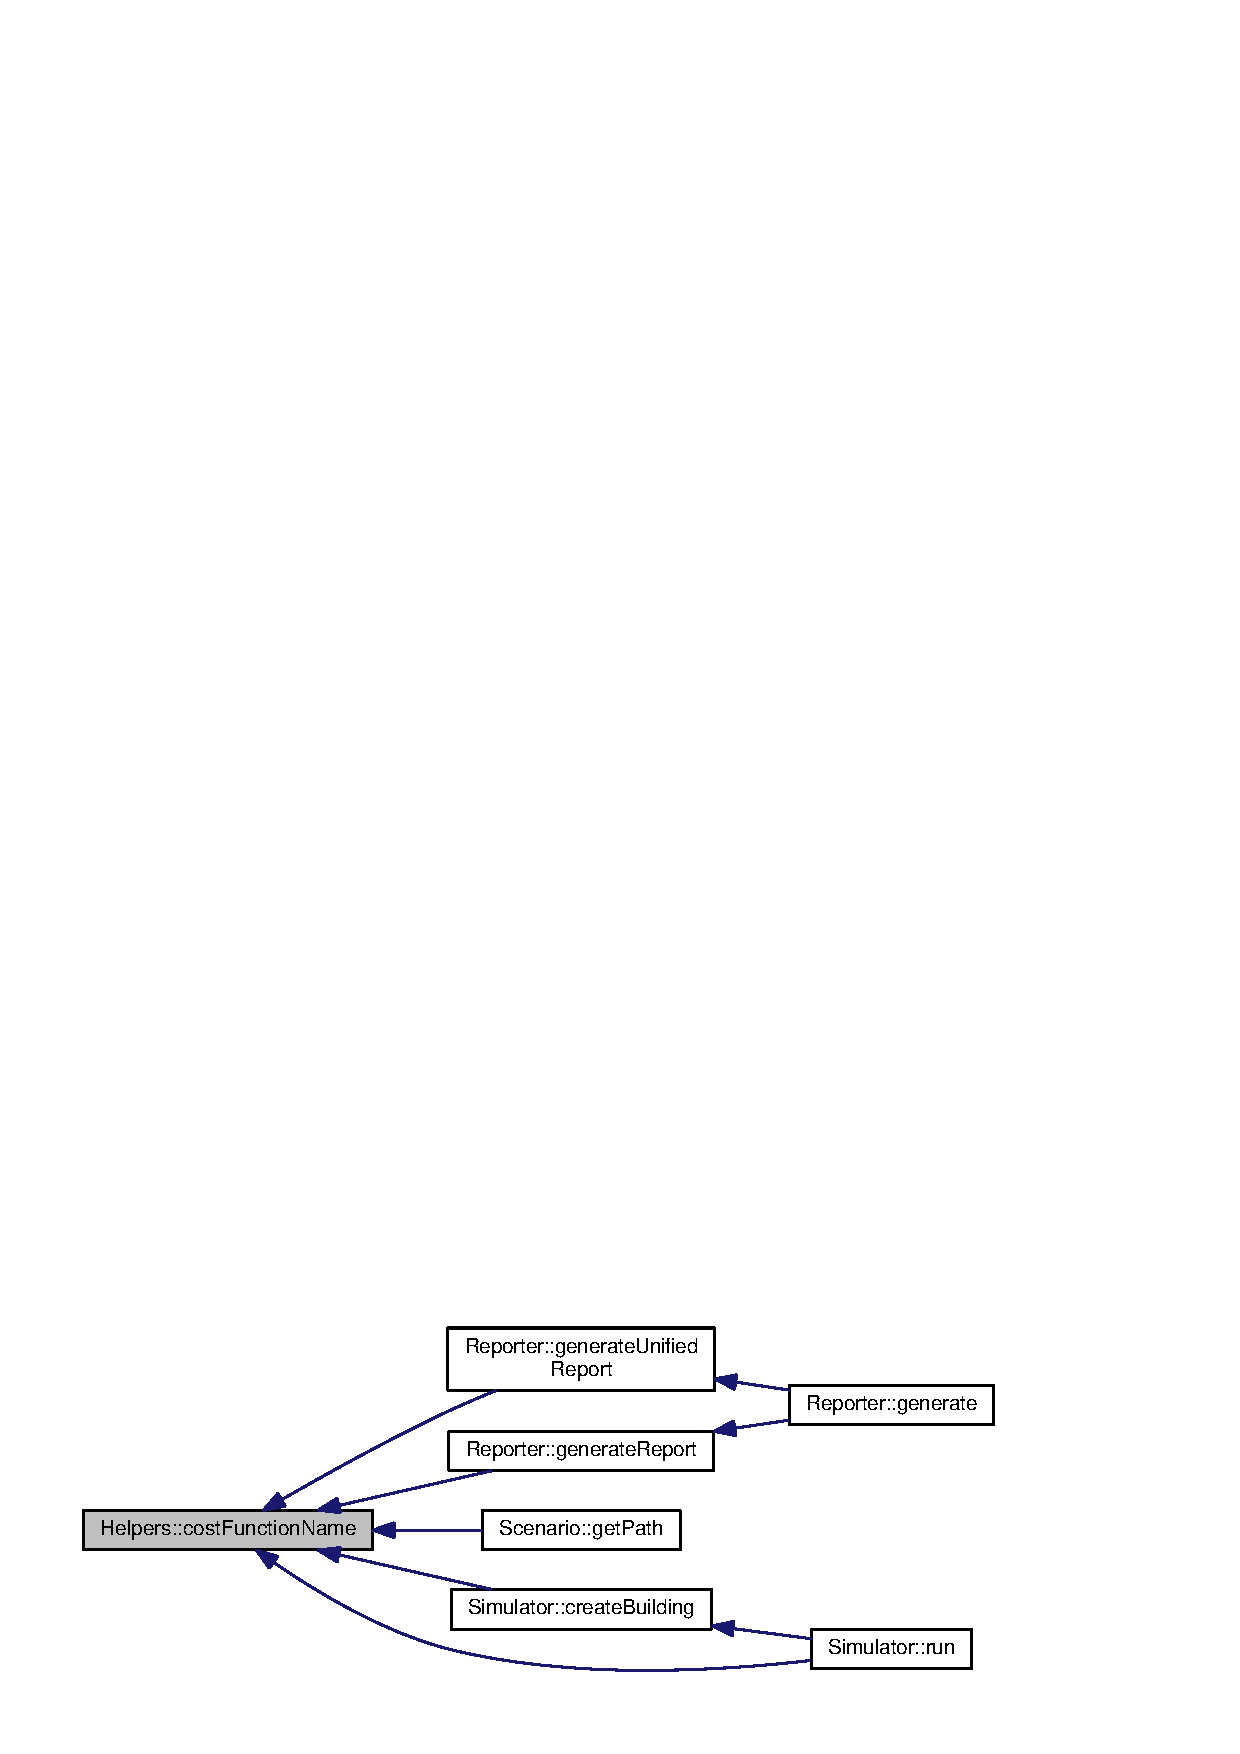
\includegraphics[width=350pt]{namespace_helpers_a51b4991513657bea83b1ad43c778aec7_icgraph}
\end{center}
\end{figure}


\index{Helpers@{Helpers}!direction\+Name@{direction\+Name}}
\index{direction\+Name@{direction\+Name}!Helpers@{Helpers}}
\subsubsection[{direction\+Name}]{\setlength{\rightskip}{0pt plus 5cm}static std\+::string Helpers\+::direction\+Name (
\begin{DoxyParamCaption}
\item[{{\bf Direction}}]{type}
\end{DoxyParamCaption}
)\hspace{0.3cm}{\ttfamily [static]}}\label{namespace_helpers_a2c85394d10f1877f982ae21bc65ee601}


Definition at line 11 of file Direction.\+h.



Here is the caller graph for this function\+:
\nopagebreak
\begin{figure}[H]
\begin{center}
\leavevmode
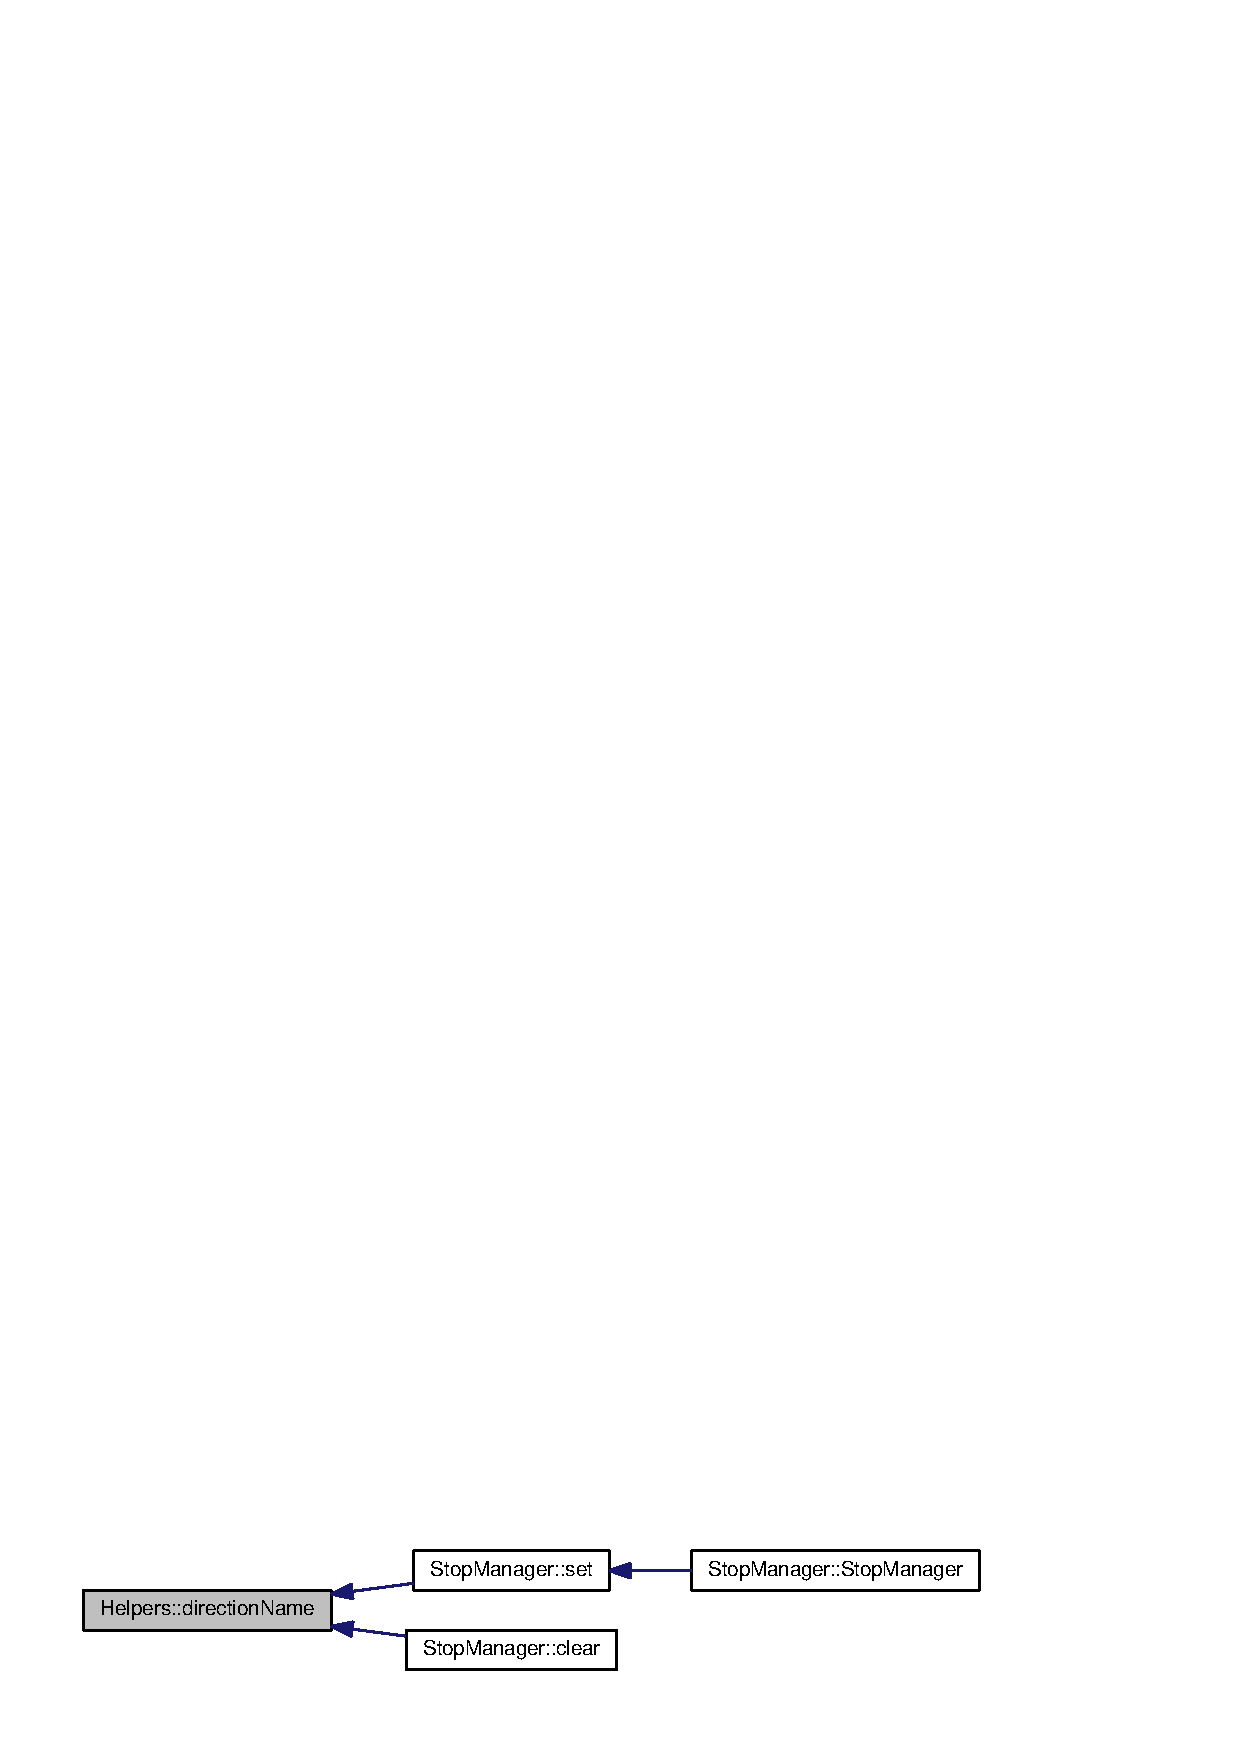
\includegraphics[width=350pt]{namespace_helpers_a2c85394d10f1877f982ae21bc65ee601_icgraph}
\end{center}
\end{figure}


\index{Helpers@{Helpers}!event\+Type\+Name@{event\+Type\+Name}}
\index{event\+Type\+Name@{event\+Type\+Name}!Helpers@{Helpers}}
\subsubsection[{event\+Type\+Name}]{\setlength{\rightskip}{0pt plus 5cm}static std\+::string Helpers\+::event\+Type\+Name (
\begin{DoxyParamCaption}
\item[{{\bf Event\+Type}}]{type}
\end{DoxyParamCaption}
)\hspace{0.3cm}{\ttfamily [static]}}\label{namespace_helpers_a1c283431309b064cf935b645e1cb2dee}


Definition at line 11 of file Event\+Type.\+h.



Here is the caller graph for this function\+:
\nopagebreak
\begin{figure}[H]
\begin{center}
\leavevmode
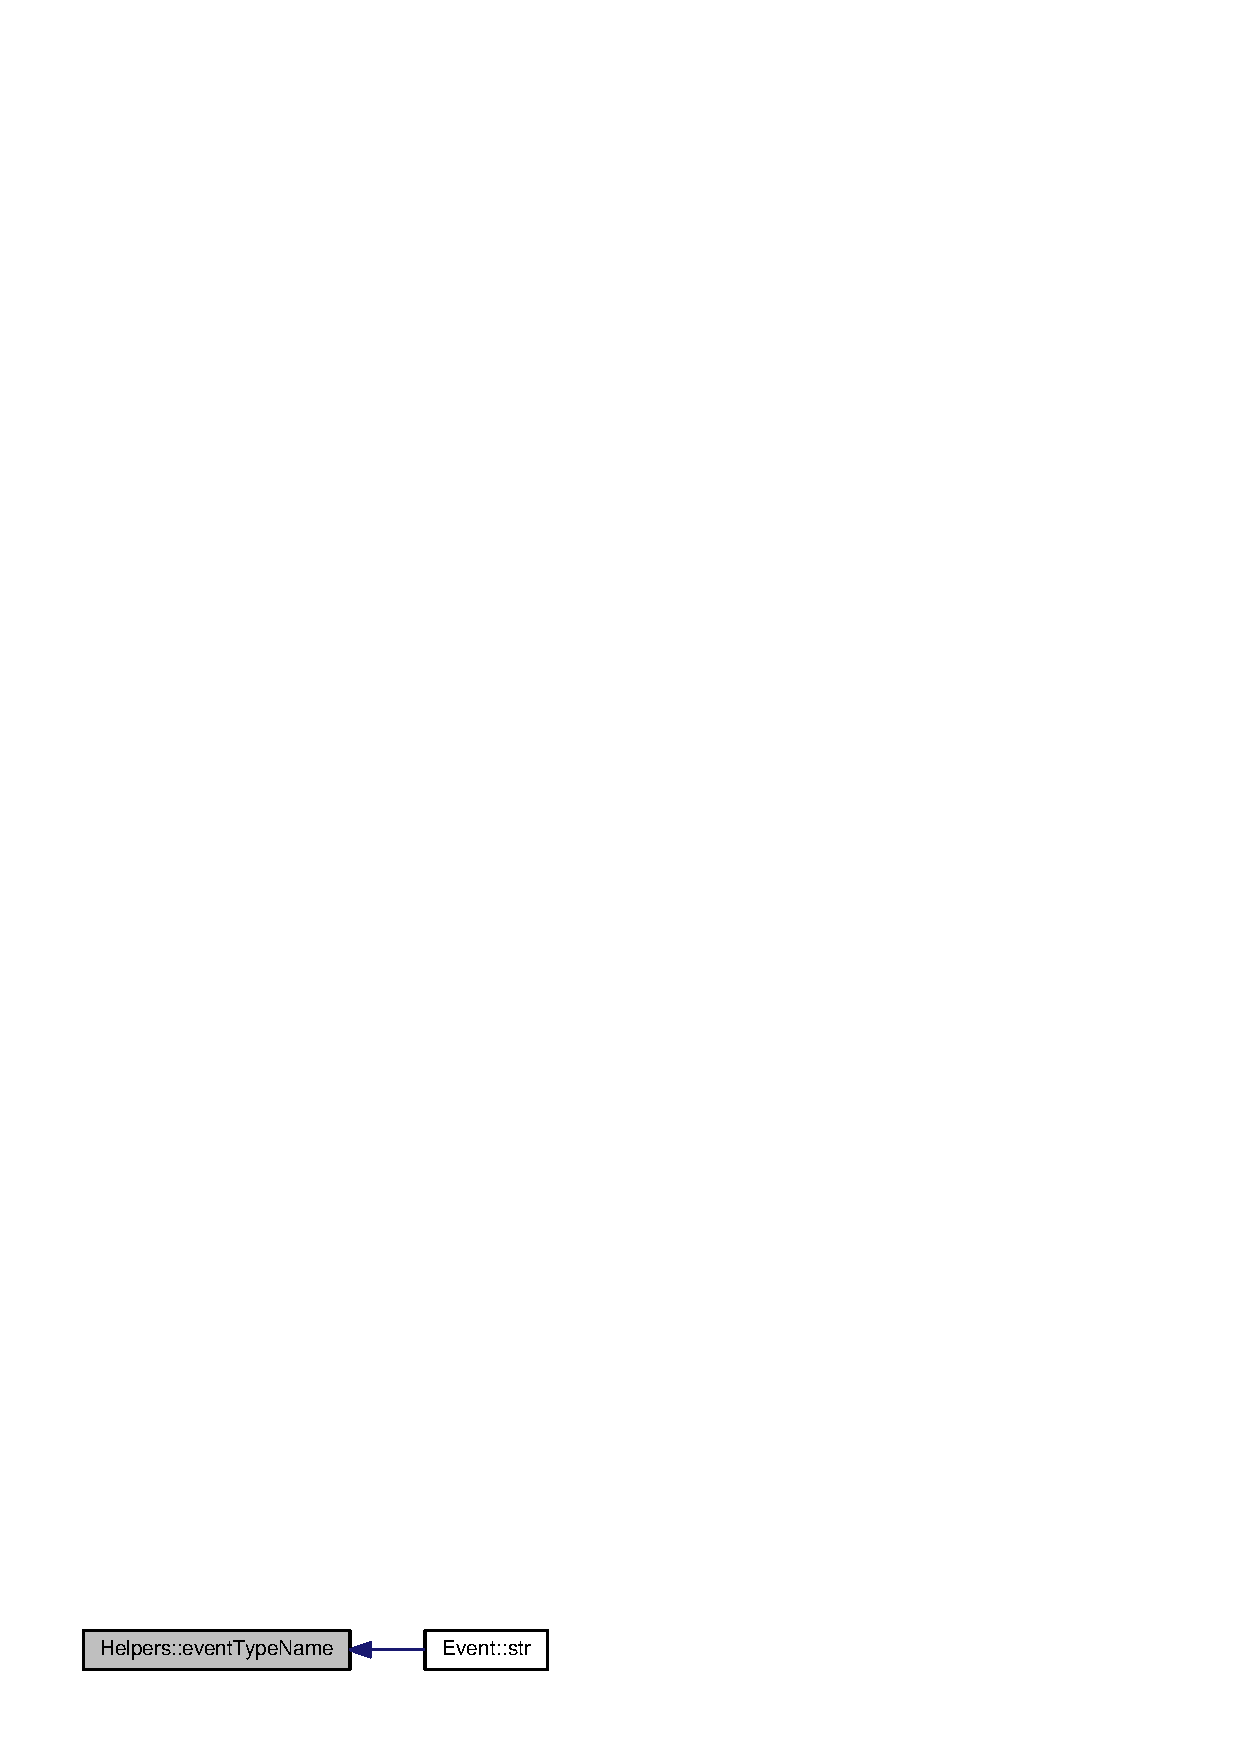
\includegraphics[width=267pt]{namespace_helpers_a1c283431309b064cf935b645e1cb2dee_icgraph}
\end{center}
\end{figure}


\index{Helpers@{Helpers}!scheduler\+Name@{scheduler\+Name}}
\index{scheduler\+Name@{scheduler\+Name}!Helpers@{Helpers}}
\subsubsection[{scheduler\+Name}]{\setlength{\rightskip}{0pt plus 5cm}static std\+::string Helpers\+::scheduler\+Name (
\begin{DoxyParamCaption}
\item[{{\bf Scheduler\+Type}}]{type}
\end{DoxyParamCaption}
)\hspace{0.3cm}{\ttfamily [static]}}\label{namespace_helpers_a6623afaa6548aa85a5a1bfd019e1e55f}


Definition at line 13 of file Scheduler\+Type.\+h.



Here is the caller graph for this function\+:
\nopagebreak
\begin{figure}[H]
\begin{center}
\leavevmode
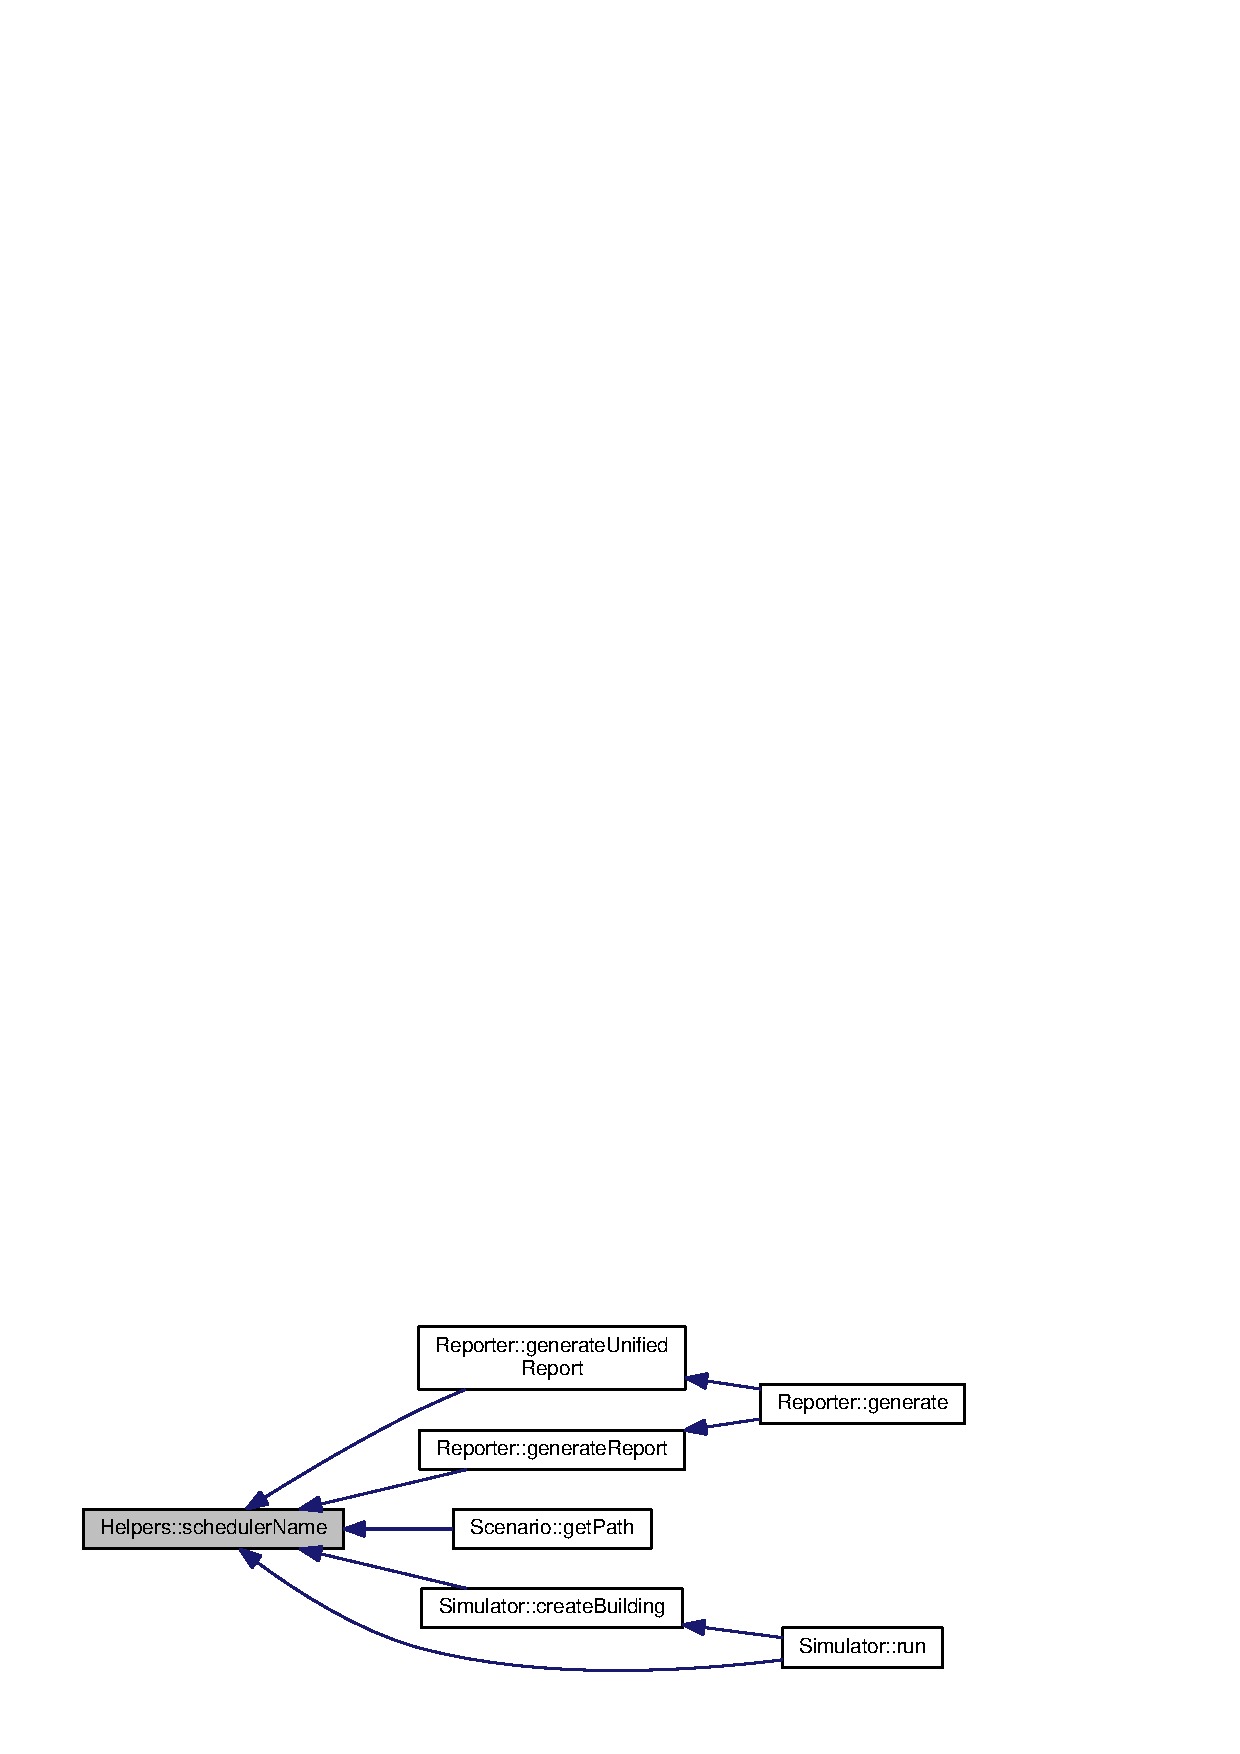
\includegraphics[width=350pt]{namespace_helpers_a6623afaa6548aa85a5a1bfd019e1e55f_icgraph}
\end{center}
\end{figure}


\index{Helpers@{Helpers}!status\+Name@{status\+Name}}
\index{status\+Name@{status\+Name}!Helpers@{Helpers}}
\subsubsection[{status\+Name}]{\setlength{\rightskip}{0pt plus 5cm}static std\+::string Helpers\+::status\+Name (
\begin{DoxyParamCaption}
\item[{{\bf Status}}]{type}
\end{DoxyParamCaption}
)\hspace{0.3cm}{\ttfamily [static]}}\label{namespace_helpers_a155c57c243ef309927648fbe98555f02}


Definition at line 15 of file Status.\+h.


\section{Y\+A\+M\+L Namespace Reference}
\label{namespace_y_a_m_l}\index{Y\+A\+M\+L@{Y\+A\+M\+L}}

\chapter{Class Documentation}
\section{Arrival Struct Reference}
\label{struct_arrival}\index{Arrival@{Arrival}}


{\ttfamily \#include $<$Arrival.\+h$>$}



Collaboration diagram for Arrival\+:\nopagebreak
\begin{figure}[H]
\begin{center}
\leavevmode
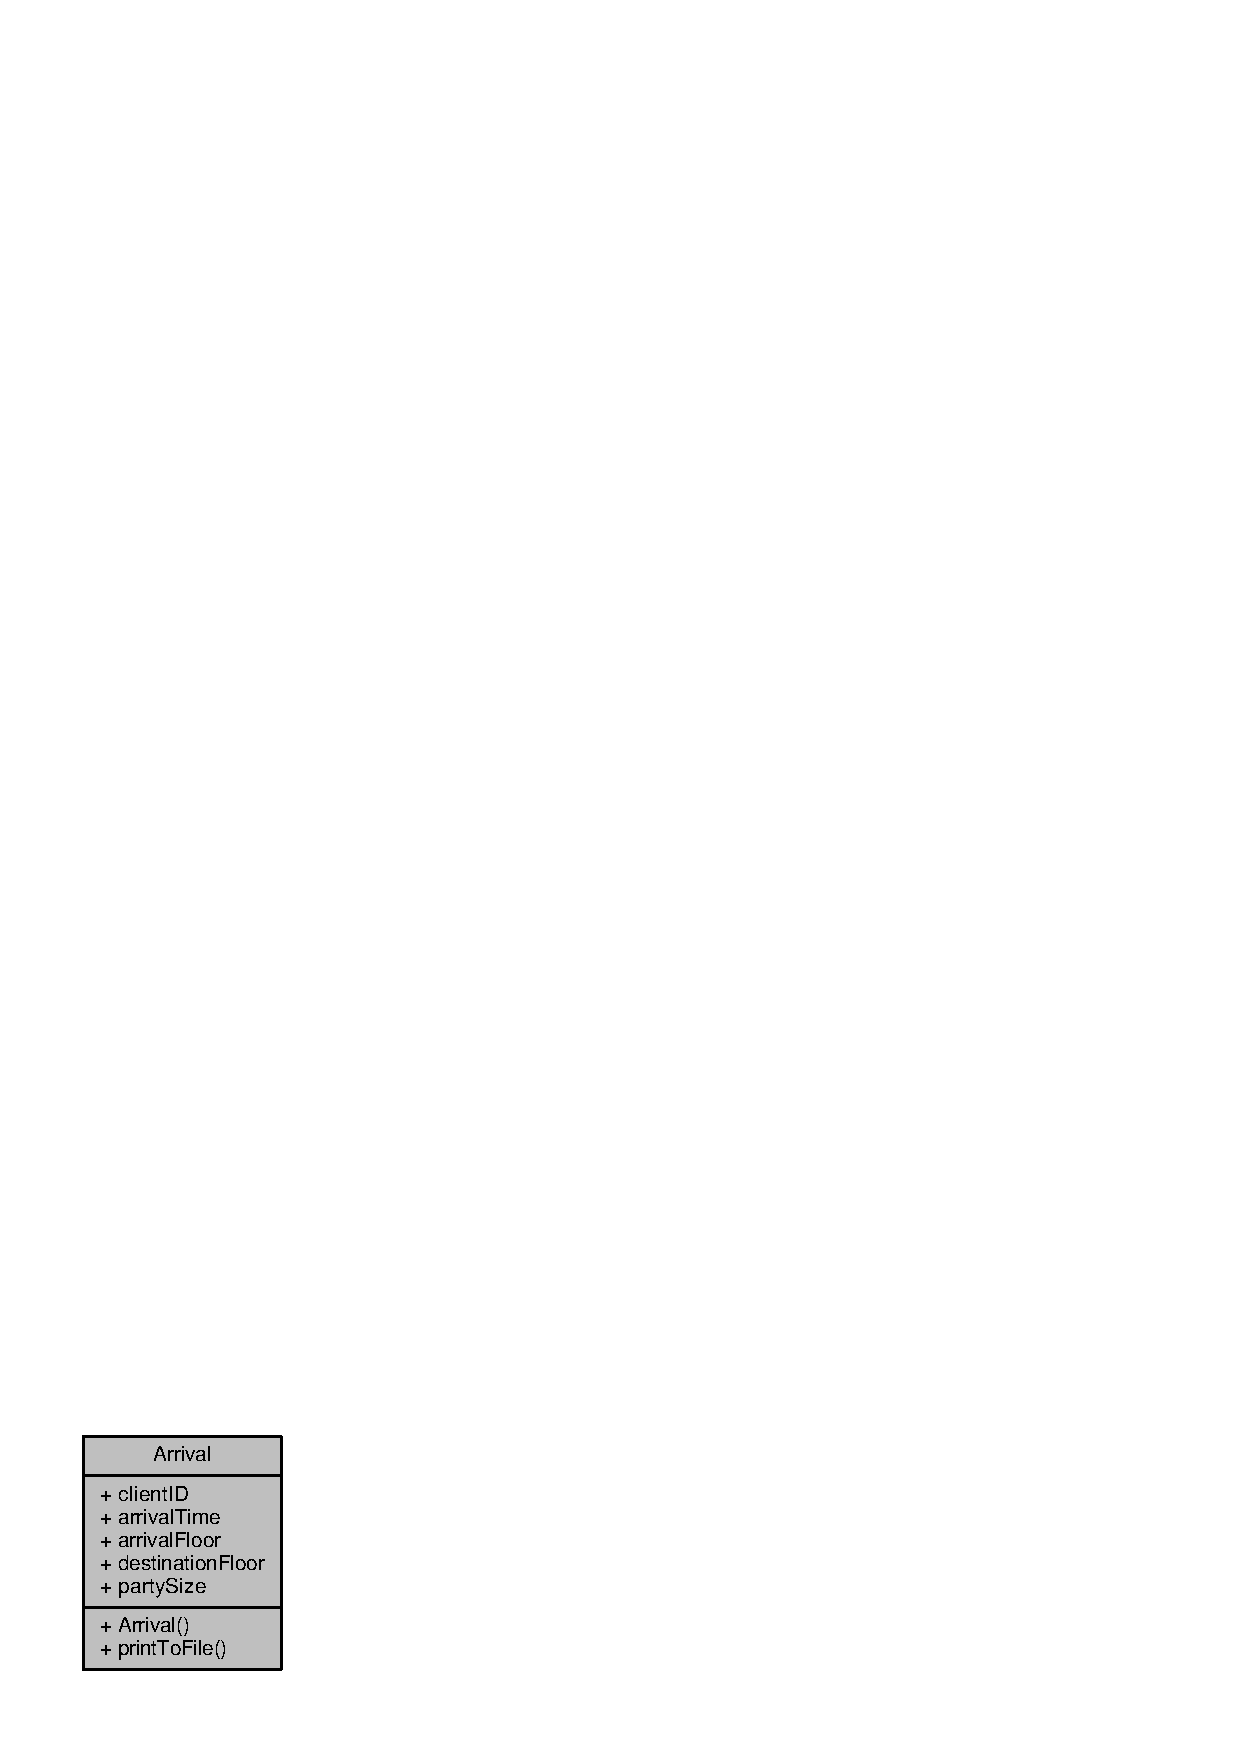
\includegraphics[width=139pt]{struct_arrival__coll__graph}
\end{center}
\end{figure}
\subsection*{Public Member Functions}
\begin{DoxyCompactItemize}
\item 
{\bf Arrival} ()
\item 
void {\bf print\+To\+File} (std\+::ofstream \&f)
\end{DoxyCompactItemize}
\subsection*{Public Attributes}
\begin{DoxyCompactItemize}
\item 
int {\bf client\+I\+D}
\item 
int {\bf arrival\+Time}
\item 
int {\bf arrival\+Floor}
\item 
int {\bf destination\+Floor}
\item 
int {\bf party\+Size}
\end{DoxyCompactItemize}


\subsection{Detailed Description}


Definition at line 5 of file Arrival.\+h.



\subsection{Constructor \& Destructor Documentation}
\index{Arrival@{Arrival}!Arrival@{Arrival}}
\index{Arrival@{Arrival}!Arrival@{Arrival}}
\subsubsection[{Arrival}]{\setlength{\rightskip}{0pt plus 5cm}Arrival\+::\+Arrival (
\begin{DoxyParamCaption}
{}
\end{DoxyParamCaption}
)}\label{struct_arrival_a5efe81eda57821d5edb6e14aa579ae8f}


Definition at line 3 of file Arrival.\+cpp.



\subsection{Member Function Documentation}
\index{Arrival@{Arrival}!print\+To\+File@{print\+To\+File}}
\index{print\+To\+File@{print\+To\+File}!Arrival@{Arrival}}
\subsubsection[{print\+To\+File}]{\setlength{\rightskip}{0pt plus 5cm}void Arrival\+::print\+To\+File (
\begin{DoxyParamCaption}
\item[{std\+::ofstream \&}]{f}
\end{DoxyParamCaption}
)}\label{struct_arrival_aca93437b96931fb116bbdaa550e58b92}


Definition at line 5 of file Arrival.\+cpp.



\subsection{Member Data Documentation}
\index{Arrival@{Arrival}!arrival\+Floor@{arrival\+Floor}}
\index{arrival\+Floor@{arrival\+Floor}!Arrival@{Arrival}}
\subsubsection[{arrival\+Floor}]{\setlength{\rightskip}{0pt plus 5cm}int Arrival\+::arrival\+Floor}\label{struct_arrival_a7037c82fd4a17d0a08d81e716fa1de5b}


Definition at line 8 of file Arrival.\+h.

\index{Arrival@{Arrival}!arrival\+Time@{arrival\+Time}}
\index{arrival\+Time@{arrival\+Time}!Arrival@{Arrival}}
\subsubsection[{arrival\+Time}]{\setlength{\rightskip}{0pt plus 5cm}int Arrival\+::arrival\+Time}\label{struct_arrival_a1604fbb65bfcc4c08cb2a4e31533dd15}


Definition at line 7 of file Arrival.\+h.

\index{Arrival@{Arrival}!client\+I\+D@{client\+I\+D}}
\index{client\+I\+D@{client\+I\+D}!Arrival@{Arrival}}
\subsubsection[{client\+I\+D}]{\setlength{\rightskip}{0pt plus 5cm}int Arrival\+::client\+I\+D}\label{struct_arrival_ad125f5bf352f24c0f02fbd25833fcbe9}


Definition at line 6 of file Arrival.\+h.

\index{Arrival@{Arrival}!destination\+Floor@{destination\+Floor}}
\index{destination\+Floor@{destination\+Floor}!Arrival@{Arrival}}
\subsubsection[{destination\+Floor}]{\setlength{\rightskip}{0pt plus 5cm}int Arrival\+::destination\+Floor}\label{struct_arrival_ae3cbceb243227c0e74011dcb04176e2f}


Definition at line 9 of file Arrival.\+h.

\index{Arrival@{Arrival}!party\+Size@{party\+Size}}
\index{party\+Size@{party\+Size}!Arrival@{Arrival}}
\subsubsection[{party\+Size}]{\setlength{\rightskip}{0pt plus 5cm}int Arrival\+::party\+Size}\label{struct_arrival_a13cb78aefa91f18325ff068a2bd4ca93}


Definition at line 10 of file Arrival.\+h.



The documentation for this struct was generated from the following files\+:\begin{DoxyCompactItemize}
\item 
include/{\bf Arrival.\+h}\item 
src/{\bf Arrival.\+cpp}\end{DoxyCompactItemize}

\hypertarget{class_better_nearest_neighbour_cost_function}{}\section{Better\+Nearest\+Neighbour\+Cost\+Function Class Reference}
\label{class_better_nearest_neighbour_cost_function}\index{Better\+Nearest\+Neighbour\+Cost\+Function@{Better\+Nearest\+Neighbour\+Cost\+Function}}


{\ttfamily \#include $<$Better\+Nearest\+Neighbour\+Cost\+Function.\+h$>$}



Inheritance diagram for Better\+Nearest\+Neighbour\+Cost\+Function\+:
\nopagebreak
\begin{figure}[H]
\begin{center}
\leavevmode
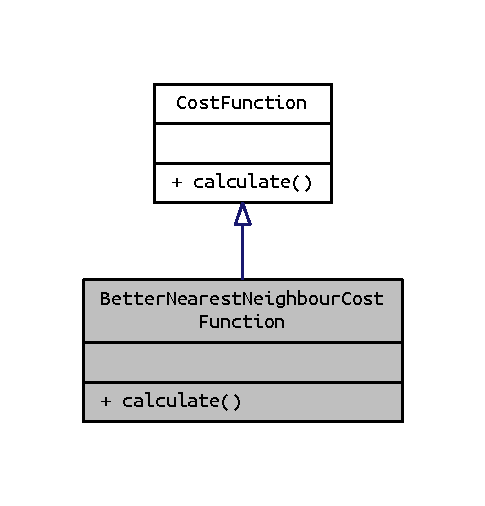
\includegraphics[width=233pt]{class_better_nearest_neighbour_cost_function__inherit__graph}
\end{center}
\end{figure}


Collaboration diagram for Better\+Nearest\+Neighbour\+Cost\+Function\+:
\nopagebreak
\begin{figure}[H]
\begin{center}
\leavevmode
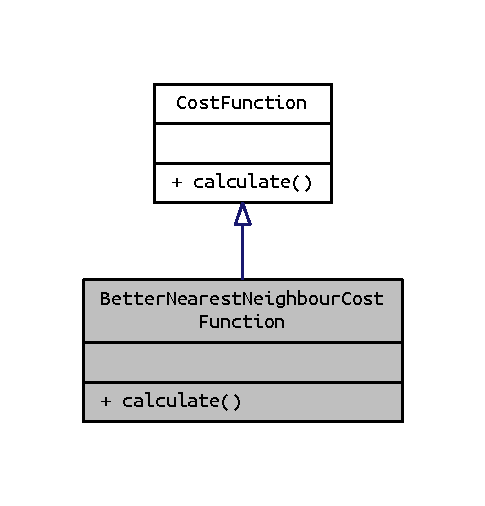
\includegraphics[width=233pt]{class_better_nearest_neighbour_cost_function__coll__graph}
\end{center}
\end{figure}
\subsection*{Public Member Functions}
\begin{DoxyCompactItemize}
\item 
float \hyperlink{class_better_nearest_neighbour_cost_function_a425ff56890dfc52fc4e0c28d8e9de5d5}{calculate} (const std\+::shared\+\_\+ptr$<$ const \hyperlink{class_building}{Building} $>$ building, const std\+::shared\+\_\+ptr$<$ const \hyperlink{class_elevator}{Elevator} $>$ elevator, const std\+::shared\+\_\+ptr$<$ const \hyperlink{class_client}{Client} $>$ client)
\end{DoxyCompactItemize}


\subsection{Member Function Documentation}
\hypertarget{class_better_nearest_neighbour_cost_function_a425ff56890dfc52fc4e0c28d8e9de5d5}{}\index{Better\+Nearest\+Neighbour\+Cost\+Function@{Better\+Nearest\+Neighbour\+Cost\+Function}!calculate@{calculate}}
\index{calculate@{calculate}!Better\+Nearest\+Neighbour\+Cost\+Function@{Better\+Nearest\+Neighbour\+Cost\+Function}}
\subsubsection[{calculate}]{\setlength{\rightskip}{0pt plus 5cm}float Better\+Nearest\+Neighbour\+Cost\+Function\+::calculate (
\begin{DoxyParamCaption}
\item[{const std\+::shared\+\_\+ptr$<$ const {\bf Building} $>$}]{building, }
\item[{const std\+::shared\+\_\+ptr$<$ const {\bf Elevator} $>$}]{elevator, }
\item[{const std\+::shared\+\_\+ptr$<$ const {\bf Client} $>$}]{client}
\end{DoxyParamCaption}
)\hspace{0.3cm}{\ttfamily [virtual]}}\label{class_better_nearest_neighbour_cost_function_a425ff56890dfc52fc4e0c28d8e9de5d5}


Implements \hyperlink{class_cost_function_ada1a1003e80f4f0e57b20d9a1e6a51c6}{Cost\+Function}.



The documentation for this class was generated from the following files\+:\begin{DoxyCompactItemize}
\item 
include/\hyperlink{_better_nearest_neighbour_cost_function_8h}{Better\+Nearest\+Neighbour\+Cost\+Function.\+h}\item 
src/\hyperlink{_better_nearest_neighbour_cost_function_8cpp}{Better\+Nearest\+Neighbour\+Cost\+Function.\+cpp}\end{DoxyCompactItemize}

\hypertarget{class_building}{}\section{Building Class Reference}
\label{class_building}\index{Building@{Building}}


{\ttfamily \#include $<$Building.\+h$>$}



Inheritance diagram for Building\+:
\nopagebreak
\begin{figure}[H]
\begin{center}
\leavevmode
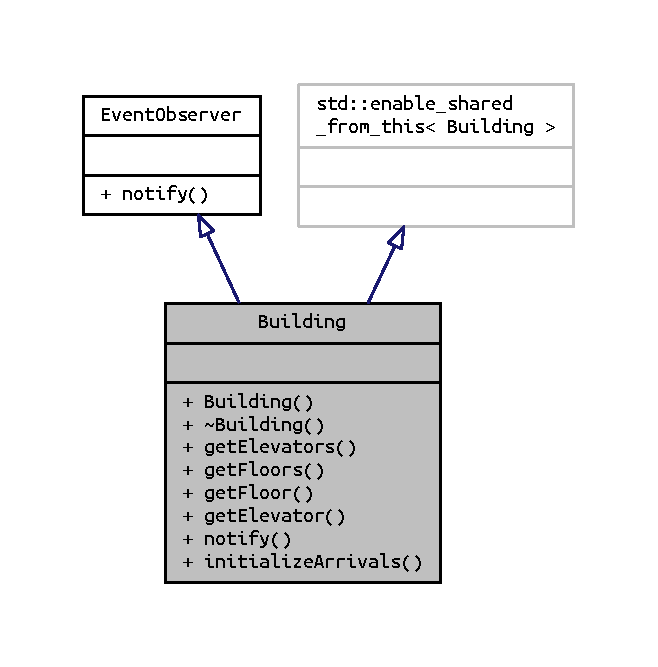
\includegraphics[width=316pt]{class_building__inherit__graph}
\end{center}
\end{figure}


Collaboration diagram for Building\+:
\nopagebreak
\begin{figure}[H]
\begin{center}
\leavevmode
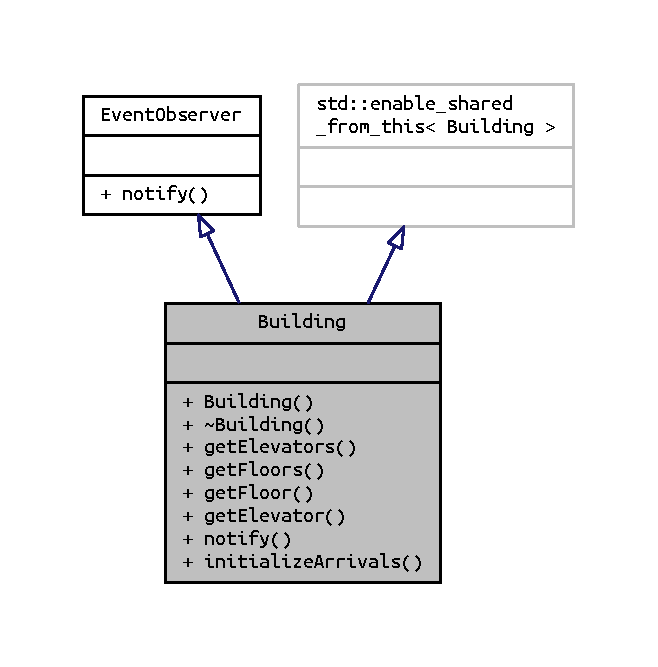
\includegraphics[width=316pt]{class_building__coll__graph}
\end{center}
\end{figure}
\subsection*{Public Member Functions}
\begin{DoxyCompactItemize}
\item 
\hyperlink{class_building_a7b82d219d50105ca73fd18fb72f7d97d}{Building} (std\+::shared\+\_\+ptr$<$ const \hyperlink{class_simulator}{Simulator} $>$ simulator, std\+::shared\+\_\+ptr$<$ std\+::vector$<$ std\+::shared\+\_\+ptr$<$ \hyperlink{class_floor}{Floor} $>$$>$$>$ floors, std\+::shared\+\_\+ptr$<$ std\+::vector$<$ std\+::shared\+\_\+ptr$<$ \hyperlink{class_elevator}{Elevator} $>$$>$$>$ elevators, std\+::shared\+\_\+ptr$<$ \hyperlink{class_scheduler}{Scheduler} $>$ scheduler, std\+::shared\+\_\+ptr$<$ \hyperlink{class_cost_function}{Cost\+Function} $>$ cost\+Function)
\item 
virtual \hyperlink{class_building_ab675c6a382e110b84031956cda708439}{$\sim$\+Building} ()
\item 
const std\+::shared\+\_\+ptr$<$ std\+::vector$<$ std\+::shared\+\_\+ptr$<$ \hyperlink{class_elevator}{Elevator} $>$ $>$ $>$ \hyperlink{class_building_a6cf389ad55a55b0d3681808025625c4a}{get\+Elevators} () const 
\item 
const std\+::shared\+\_\+ptr$<$ std\+::vector$<$ std\+::shared\+\_\+ptr$<$ \hyperlink{class_floor}{Floor} $>$ $>$ $>$ \hyperlink{class_building_a1271cef8df030a441d37eec8f8245928}{get\+Floors} () const 
\item 
const std\+::shared\+\_\+ptr$<$ \hyperlink{class_floor}{Floor} $>$ \hyperlink{class_building_a55712da518a32920146db267072362f2}{get\+Floor} (int number) const 
\item 
const std\+::shared\+\_\+ptr$<$ \hyperlink{class_elevator}{Elevator} $>$ \hyperlink{class_building_aea6f1c1241ae910793a4a80bf0cadc02}{get\+Elevator} (int number) const 
\item 
void \hyperlink{class_building_a380e65fcb24d40d82077edc0572df3c1}{notify} (const std\+::shared\+\_\+ptr$<$ const \hyperlink{class_event}{Event} $>$ event)
\item 
void \hyperlink{class_building_ad92eb27909cc8e59a2a775d7b214d13c}{initialize\+Arrivals} ()
\end{DoxyCompactItemize}


\subsection{Constructor \& Destructor Documentation}
\hypertarget{class_building_a7b82d219d50105ca73fd18fb72f7d97d}{}\index{Building@{Building}!Building@{Building}}
\index{Building@{Building}!Building@{Building}}
\subsubsection[{Building}]{\setlength{\rightskip}{0pt plus 5cm}Building\+::\+Building (
\begin{DoxyParamCaption}
\item[{std\+::shared\+\_\+ptr$<$ const {\bf Simulator} $>$}]{simulator, }
\item[{std\+::shared\+\_\+ptr$<$ std\+::vector$<$ std\+::shared\+\_\+ptr$<$ {\bf Floor} $>$$>$$>$}]{floors, }
\item[{std\+::shared\+\_\+ptr$<$ std\+::vector$<$ std\+::shared\+\_\+ptr$<$ {\bf Elevator} $>$$>$$>$}]{elevators, }
\item[{std\+::shared\+\_\+ptr$<$ {\bf Scheduler} $>$}]{scheduler, }
\item[{std\+::shared\+\_\+ptr$<$ {\bf Cost\+Function} $>$}]{cost\+Function}
\end{DoxyParamCaption}
)}\label{class_building_a7b82d219d50105ca73fd18fb72f7d97d}
\hypertarget{class_building_ab675c6a382e110b84031956cda708439}{}\index{Building@{Building}!````~Building@{$\sim$\+Building}}
\index{````~Building@{$\sim$\+Building}!Building@{Building}}
\subsubsection[{$\sim$\+Building}]{\setlength{\rightskip}{0pt plus 5cm}Building\+::$\sim$\+Building (
\begin{DoxyParamCaption}
{}
\end{DoxyParamCaption}
)\hspace{0.3cm}{\ttfamily [virtual]}}\label{class_building_ab675c6a382e110b84031956cda708439}


\subsection{Member Function Documentation}
\hypertarget{class_building_aea6f1c1241ae910793a4a80bf0cadc02}{}\index{Building@{Building}!get\+Elevator@{get\+Elevator}}
\index{get\+Elevator@{get\+Elevator}!Building@{Building}}
\subsubsection[{get\+Elevator}]{\setlength{\rightskip}{0pt plus 5cm}const std\+::shared\+\_\+ptr$<$ {\bf Elevator} $>$ Building\+::get\+Elevator (
\begin{DoxyParamCaption}
\item[{int}]{number}
\end{DoxyParamCaption}
) const}\label{class_building_aea6f1c1241ae910793a4a80bf0cadc02}
\hypertarget{class_building_a6cf389ad55a55b0d3681808025625c4a}{}\index{Building@{Building}!get\+Elevators@{get\+Elevators}}
\index{get\+Elevators@{get\+Elevators}!Building@{Building}}
\subsubsection[{get\+Elevators}]{\setlength{\rightskip}{0pt plus 5cm}const std\+::shared\+\_\+ptr$<$ std\+::vector$<$ std\+::shared\+\_\+ptr$<$ {\bf Elevator} $>$ $>$ $>$ Building\+::get\+Elevators (
\begin{DoxyParamCaption}
{}
\end{DoxyParamCaption}
) const}\label{class_building_a6cf389ad55a55b0d3681808025625c4a}
\hypertarget{class_building_a55712da518a32920146db267072362f2}{}\index{Building@{Building}!get\+Floor@{get\+Floor}}
\index{get\+Floor@{get\+Floor}!Building@{Building}}
\subsubsection[{get\+Floor}]{\setlength{\rightskip}{0pt plus 5cm}const std\+::shared\+\_\+ptr$<$ {\bf Floor} $>$ Building\+::get\+Floor (
\begin{DoxyParamCaption}
\item[{int}]{number}
\end{DoxyParamCaption}
) const}\label{class_building_a55712da518a32920146db267072362f2}
\hypertarget{class_building_a1271cef8df030a441d37eec8f8245928}{}\index{Building@{Building}!get\+Floors@{get\+Floors}}
\index{get\+Floors@{get\+Floors}!Building@{Building}}
\subsubsection[{get\+Floors}]{\setlength{\rightskip}{0pt plus 5cm}const std\+::shared\+\_\+ptr$<$ std\+::vector$<$ std\+::shared\+\_\+ptr$<$ {\bf Floor} $>$ $>$ $>$ Building\+::get\+Floors (
\begin{DoxyParamCaption}
{}
\end{DoxyParamCaption}
) const}\label{class_building_a1271cef8df030a441d37eec8f8245928}
\hypertarget{class_building_ad92eb27909cc8e59a2a775d7b214d13c}{}\index{Building@{Building}!initialize\+Arrivals@{initialize\+Arrivals}}
\index{initialize\+Arrivals@{initialize\+Arrivals}!Building@{Building}}
\subsubsection[{initialize\+Arrivals}]{\setlength{\rightskip}{0pt plus 5cm}void Building\+::initialize\+Arrivals (
\begin{DoxyParamCaption}
{}
\end{DoxyParamCaption}
)}\label{class_building_ad92eb27909cc8e59a2a775d7b214d13c}
\hypertarget{class_building_a380e65fcb24d40d82077edc0572df3c1}{}\index{Building@{Building}!notify@{notify}}
\index{notify@{notify}!Building@{Building}}
\subsubsection[{notify}]{\setlength{\rightskip}{0pt plus 5cm}void Building\+::notify (
\begin{DoxyParamCaption}
\item[{const std\+::shared\+\_\+ptr$<$ const {\bf Event} $>$}]{event}
\end{DoxyParamCaption}
)\hspace{0.3cm}{\ttfamily [virtual]}}\label{class_building_a380e65fcb24d40d82077edc0572df3c1}


Implements \hyperlink{class_event_observer_a81b3c545084ba3c8eaa8c83f5a0a4eb8}{Event\+Observer}.



The documentation for this class was generated from the following files\+:\begin{DoxyCompactItemize}
\item 
include/\hyperlink{_building_8h}{Building.\+h}\item 
src/\hyperlink{_building_8cpp}{Building.\+cpp}\end{DoxyCompactItemize}

\section{Client Class Reference}
\label{class_client}\index{Client@{Client}}


{\ttfamily \#include $<$Client.\+h$>$}



Collaboration diagram for Client\+:
\nopagebreak
\begin{figure}[H]
\begin{center}
\leavevmode
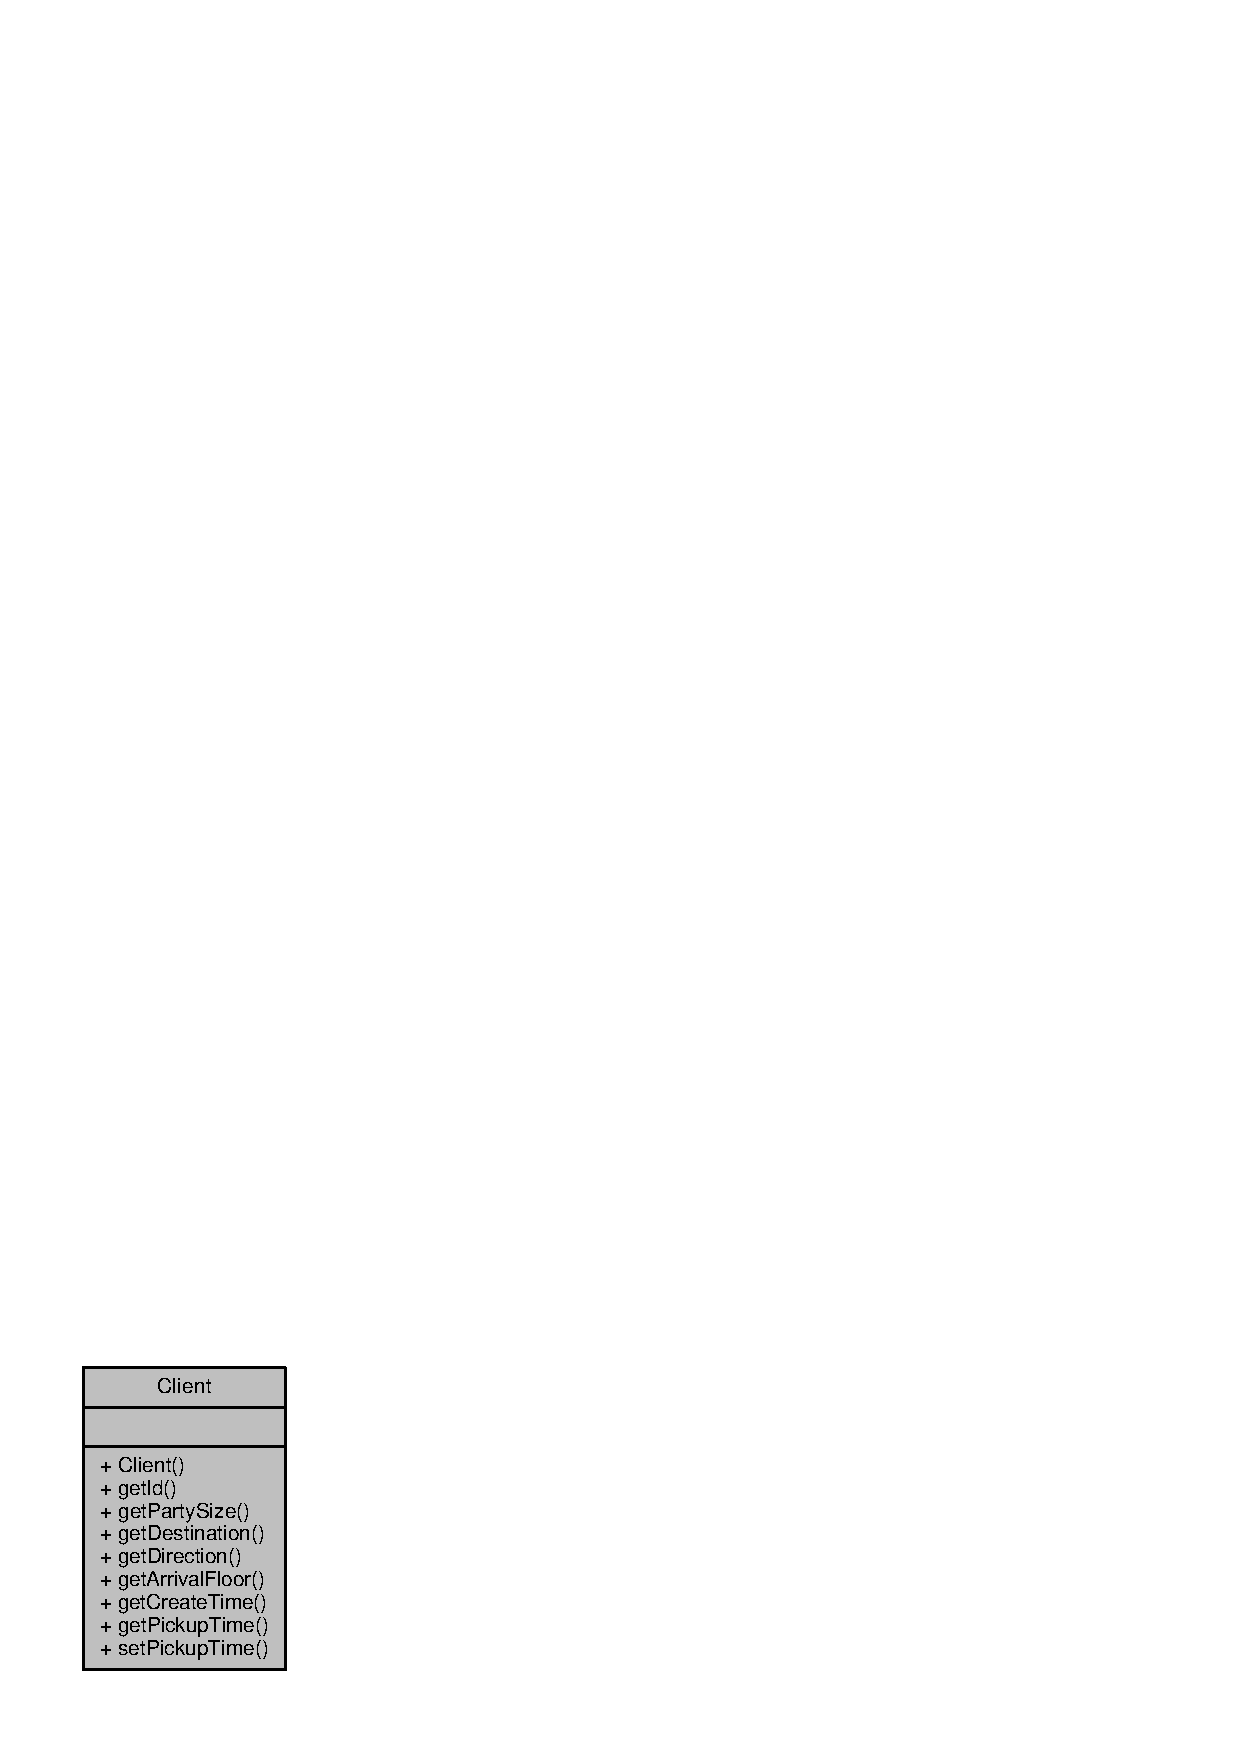
\includegraphics[width=141pt]{class_client__coll__graph}
\end{center}
\end{figure}
\subsection*{Public Member Functions}
\begin{DoxyCompactItemize}
\item 
{\bf Client} (const int party\+Size, const int arrival\+Floor, const int destination, const unsigned long create\+Time)
\item 
const unsigned long {\bf get\+Id} () const 
\item 
const int {\bf get\+Party\+Size} () const 
\item 
const int {\bf get\+Destination} () const 
\item 
const {\bf Direction} {\bf get\+Direction} () const 
\item 
const int {\bf get\+Arrival\+Floor} () const 
\item 
const long {\bf get\+Create\+Time} () const 
\item 
const long {\bf get\+Pickup\+Time} () const 
\item 
void {\bf set\+Pickup\+Time} (const unsigned long p)
\end{DoxyCompactItemize}


\subsection{Detailed Description}


Definition at line 9 of file Client.\+h.



\subsection{Constructor \& Destructor Documentation}
\index{Client@{Client}!Client@{Client}}
\index{Client@{Client}!Client@{Client}}
\subsubsection[{Client}]{\setlength{\rightskip}{0pt plus 5cm}Client\+::\+Client (
\begin{DoxyParamCaption}
\item[{const int}]{party\+Size, }
\item[{const int}]{arrival\+Floor, }
\item[{const int}]{destination, }
\item[{const unsigned long}]{create\+Time}
\end{DoxyParamCaption}
)}\label{class_client_a6407dd19f039e827716a2190d29775f6}


Definition at line 7 of file Client.\+cpp.



\subsection{Member Function Documentation}
\index{Client@{Client}!get\+Arrival\+Floor@{get\+Arrival\+Floor}}
\index{get\+Arrival\+Floor@{get\+Arrival\+Floor}!Client@{Client}}
\subsubsection[{get\+Arrival\+Floor}]{\setlength{\rightskip}{0pt plus 5cm}const int Client\+::get\+Arrival\+Floor (
\begin{DoxyParamCaption}
{}
\end{DoxyParamCaption}
) const}\label{class_client_a08e69644c23ed38659a5f10f4fe5a710}


Definition at line 25 of file Client.\+cpp.

\index{Client@{Client}!get\+Create\+Time@{get\+Create\+Time}}
\index{get\+Create\+Time@{get\+Create\+Time}!Client@{Client}}
\subsubsection[{get\+Create\+Time}]{\setlength{\rightskip}{0pt plus 5cm}const long Client\+::get\+Create\+Time (
\begin{DoxyParamCaption}
{}
\end{DoxyParamCaption}
) const}\label{class_client_ac97f12c81f53b185d04bb99d55ad7994}


Definition at line 27 of file Client.\+cpp.

\index{Client@{Client}!get\+Destination@{get\+Destination}}
\index{get\+Destination@{get\+Destination}!Client@{Client}}
\subsubsection[{get\+Destination}]{\setlength{\rightskip}{0pt plus 5cm}const int Client\+::get\+Destination (
\begin{DoxyParamCaption}
{}
\end{DoxyParamCaption}
) const}\label{class_client_a6a596c85feaf3f7dc14c2e90e30a1979}


Definition at line 16 of file Client.\+cpp.

\index{Client@{Client}!get\+Direction@{get\+Direction}}
\index{get\+Direction@{get\+Direction}!Client@{Client}}
\subsubsection[{get\+Direction}]{\setlength{\rightskip}{0pt plus 5cm}const {\bf Direction} Client\+::get\+Direction (
\begin{DoxyParamCaption}
{}
\end{DoxyParamCaption}
) const}\label{class_client_a23944e6775bcce17d2127f6f31ccaa5b}


Definition at line 18 of file Client.\+cpp.

\index{Client@{Client}!get\+Id@{get\+Id}}
\index{get\+Id@{get\+Id}!Client@{Client}}
\subsubsection[{get\+Id}]{\setlength{\rightskip}{0pt plus 5cm}const unsigned long Client\+::get\+Id (
\begin{DoxyParamCaption}
{}
\end{DoxyParamCaption}
) const}\label{class_client_af0e6d1f2202d211d8bb4fdf17e805a17}


Definition at line 12 of file Client.\+cpp.

\index{Client@{Client}!get\+Party\+Size@{get\+Party\+Size}}
\index{get\+Party\+Size@{get\+Party\+Size}!Client@{Client}}
\subsubsection[{get\+Party\+Size}]{\setlength{\rightskip}{0pt plus 5cm}const int Client\+::get\+Party\+Size (
\begin{DoxyParamCaption}
{}
\end{DoxyParamCaption}
) const}\label{class_client_a136e2ca6d4a93f5bcb3bd8fe35f406bc}


Definition at line 14 of file Client.\+cpp.

\index{Client@{Client}!get\+Pickup\+Time@{get\+Pickup\+Time}}
\index{get\+Pickup\+Time@{get\+Pickup\+Time}!Client@{Client}}
\subsubsection[{get\+Pickup\+Time}]{\setlength{\rightskip}{0pt plus 5cm}const long Client\+::get\+Pickup\+Time (
\begin{DoxyParamCaption}
{}
\end{DoxyParamCaption}
) const}\label{class_client_a6f56a7f9c471bd34800c67a2a0e135a9}


Definition at line 29 of file Client.\+cpp.

\index{Client@{Client}!set\+Pickup\+Time@{set\+Pickup\+Time}}
\index{set\+Pickup\+Time@{set\+Pickup\+Time}!Client@{Client}}
\subsubsection[{set\+Pickup\+Time}]{\setlength{\rightskip}{0pt plus 5cm}void Client\+::set\+Pickup\+Time (
\begin{DoxyParamCaption}
\item[{const unsigned long}]{p}
\end{DoxyParamCaption}
)}\label{class_client_a7988e646af304d1b62a2d8495d53a34d}


Definition at line 31 of file Client.\+cpp.



The documentation for this class was generated from the following files\+:\begin{DoxyCompactItemize}
\item 
include/{\bf Client.\+h}\item 
src/{\bf Client.\+cpp}\end{DoxyCompactItemize}

\hypertarget{class_client_arrival}{}\section{Client\+Arrival Class Reference}
\label{class_client_arrival}\index{Client\+Arrival@{Client\+Arrival}}


{\ttfamily \#include $<$Client\+Arrival.\+h$>$}



Inheritance diagram for Client\+Arrival\+:
\nopagebreak
\begin{figure}[H]
\begin{center}
\leavevmode
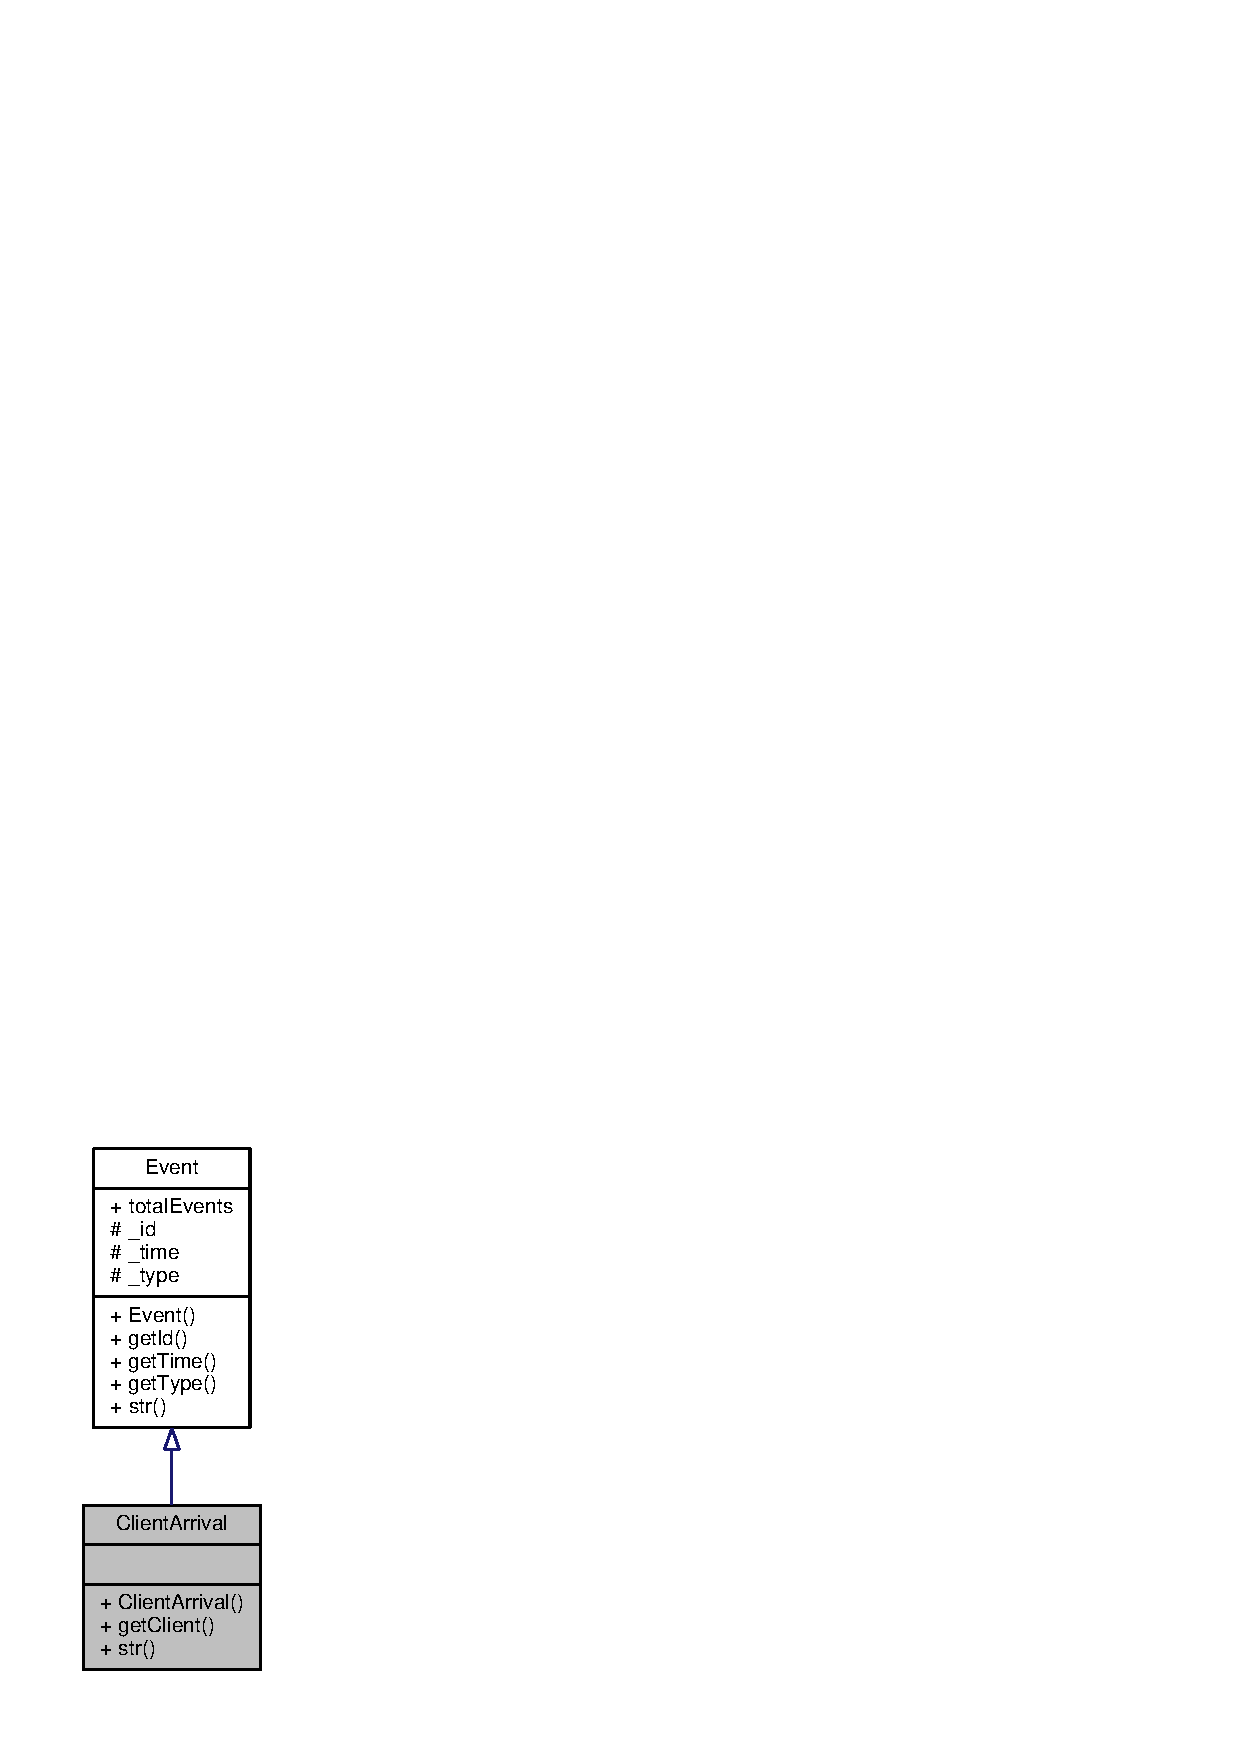
\includegraphics[width=186pt]{class_client_arrival__inherit__graph}
\end{center}
\end{figure}


Collaboration diagram for Client\+Arrival\+:
\nopagebreak
\begin{figure}[H]
\begin{center}
\leavevmode
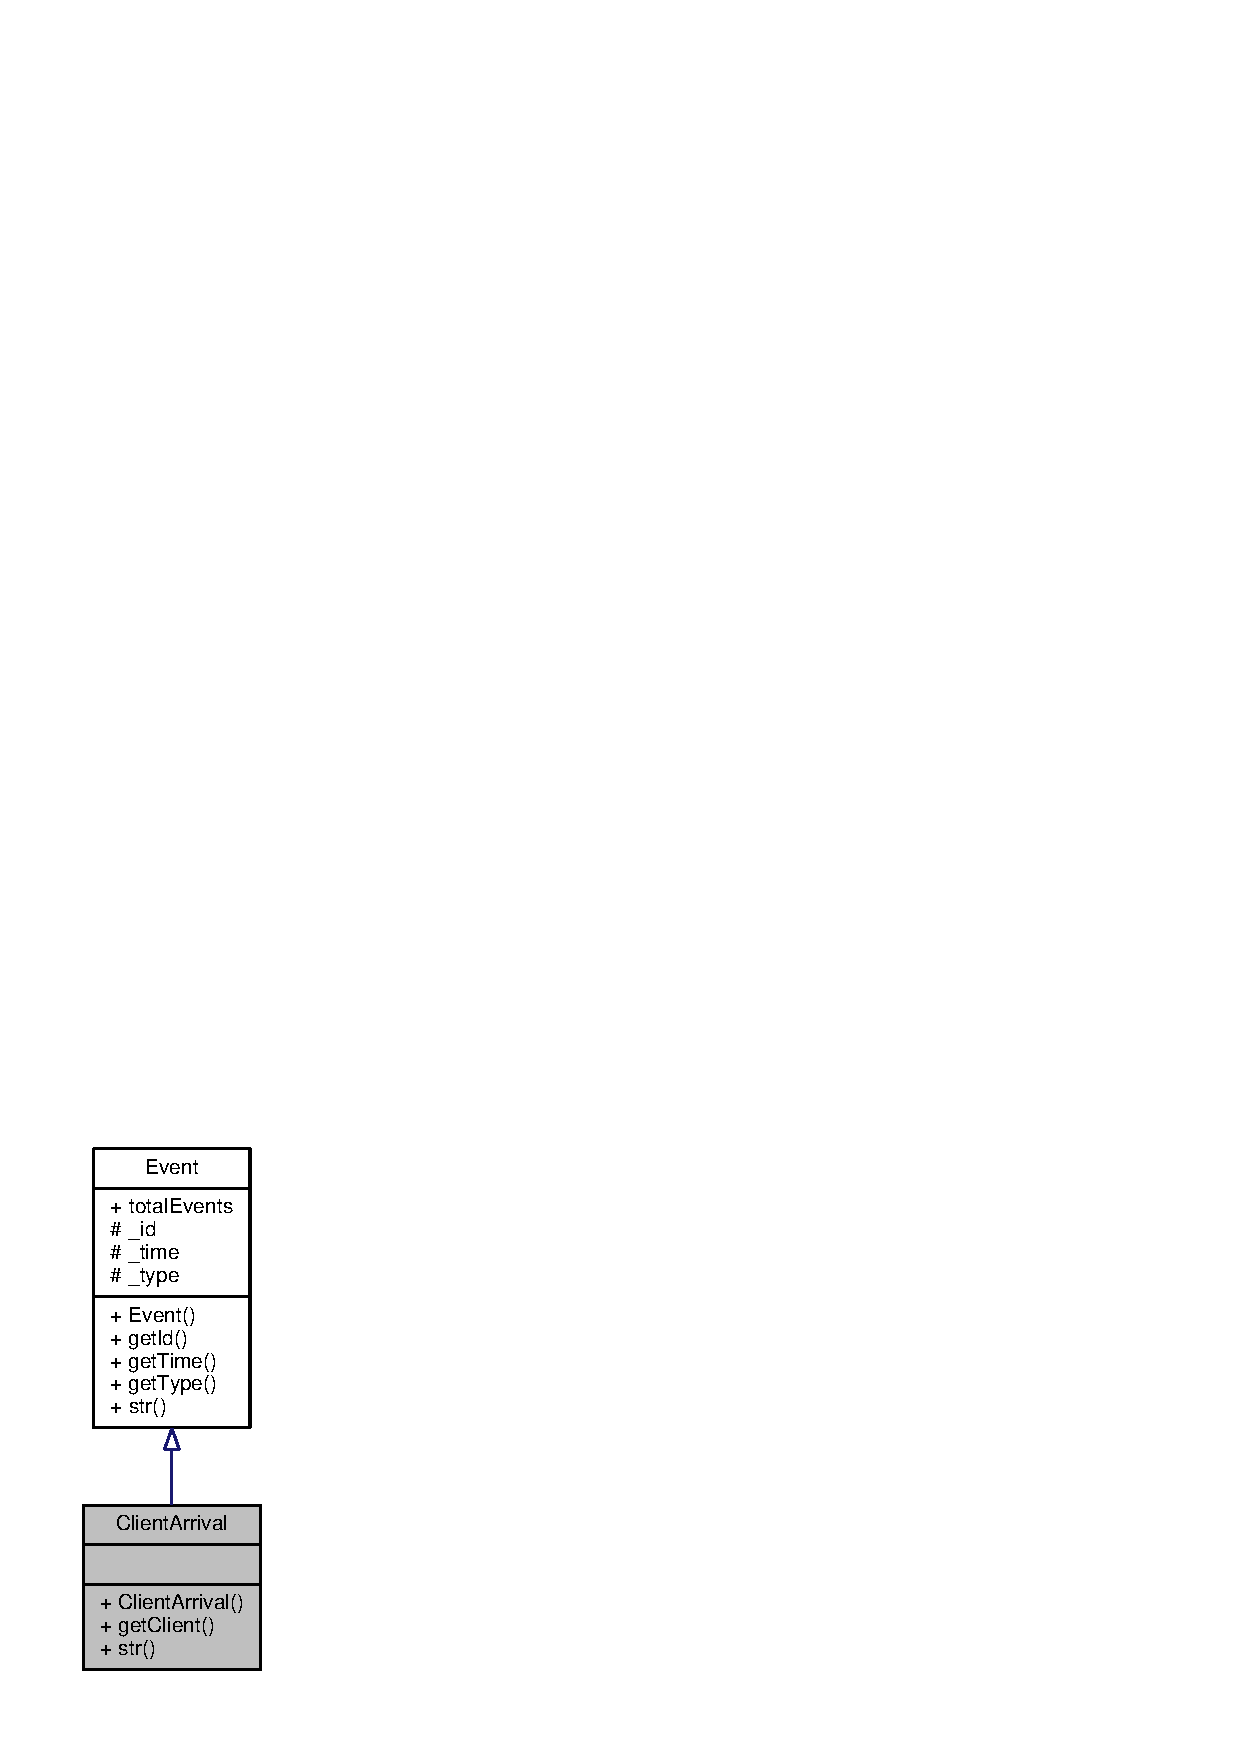
\includegraphics[width=186pt]{class_client_arrival__coll__graph}
\end{center}
\end{figure}
\subsection*{Public Member Functions}
\begin{DoxyCompactItemize}
\item 
\hyperlink{class_client_arrival_adcf0616ba427c6232c797cd1c3be3590}{Client\+Arrival} (const unsigned long event\+Time, const std\+::shared\+\_\+ptr$<$ \hyperlink{class_client}{Client} $>$ client)
\item 
const std\+::shared\+\_\+ptr$<$ \hyperlink{class_client}{Client} $>$ \hyperlink{class_client_arrival_a0e83b6899e3867658427ab2e26e3060a}{get\+Client} () const 
\item 
std\+::string \hyperlink{class_client_arrival_aed100adfc8eaf083194ac0c630eaafe6}{str} () const 
\end{DoxyCompactItemize}
\subsection*{Additional Inherited Members}


\subsection{Constructor \& Destructor Documentation}
\hypertarget{class_client_arrival_adcf0616ba427c6232c797cd1c3be3590}{}\index{Client\+Arrival@{Client\+Arrival}!Client\+Arrival@{Client\+Arrival}}
\index{Client\+Arrival@{Client\+Arrival}!Client\+Arrival@{Client\+Arrival}}
\subsubsection[{Client\+Arrival}]{\setlength{\rightskip}{0pt plus 5cm}Client\+Arrival\+::\+Client\+Arrival (
\begin{DoxyParamCaption}
\item[{const unsigned long}]{event\+Time, }
\item[{const std\+::shared\+\_\+ptr$<$ {\bf Client} $>$}]{client}
\end{DoxyParamCaption}
)}\label{class_client_arrival_adcf0616ba427c6232c797cd1c3be3590}


\subsection{Member Function Documentation}
\hypertarget{class_client_arrival_a0e83b6899e3867658427ab2e26e3060a}{}\index{Client\+Arrival@{Client\+Arrival}!get\+Client@{get\+Client}}
\index{get\+Client@{get\+Client}!Client\+Arrival@{Client\+Arrival}}
\subsubsection[{get\+Client}]{\setlength{\rightskip}{0pt plus 5cm}const std\+::shared\+\_\+ptr$<$ {\bf Client} $>$ Client\+Arrival\+::get\+Client (
\begin{DoxyParamCaption}
{}
\end{DoxyParamCaption}
) const}\label{class_client_arrival_a0e83b6899e3867658427ab2e26e3060a}
\hypertarget{class_client_arrival_aed100adfc8eaf083194ac0c630eaafe6}{}\index{Client\+Arrival@{Client\+Arrival}!str@{str}}
\index{str@{str}!Client\+Arrival@{Client\+Arrival}}
\subsubsection[{str}]{\setlength{\rightskip}{0pt plus 5cm}std\+::string Client\+Arrival\+::str (
\begin{DoxyParamCaption}
{}
\end{DoxyParamCaption}
) const\hspace{0.3cm}{\ttfamily [virtual]}}\label{class_client_arrival_aed100adfc8eaf083194ac0c630eaafe6}


Reimplemented from \hyperlink{class_event_abf16ed4a9c78514c704ce2de6a2b9ec7}{Event}.



The documentation for this class was generated from the following files\+:\begin{DoxyCompactItemize}
\item 
include/\hyperlink{_client_arrival_8h}{Client\+Arrival.\+h}\item 
src/\hyperlink{_client_arrival_8cpp}{Client\+Arrival.\+cpp}\end{DoxyCompactItemize}

\section{Client\+Comparator Class Reference}
\label{class_client_comparator}\index{Client\+Comparator@{Client\+Comparator}}


{\ttfamily \#include $<$Planning\+Scheduler.\+h$>$}



Collaboration diagram for Client\+Comparator\+:
\nopagebreak
\begin{figure}[H]
\begin{center}
\leavevmode
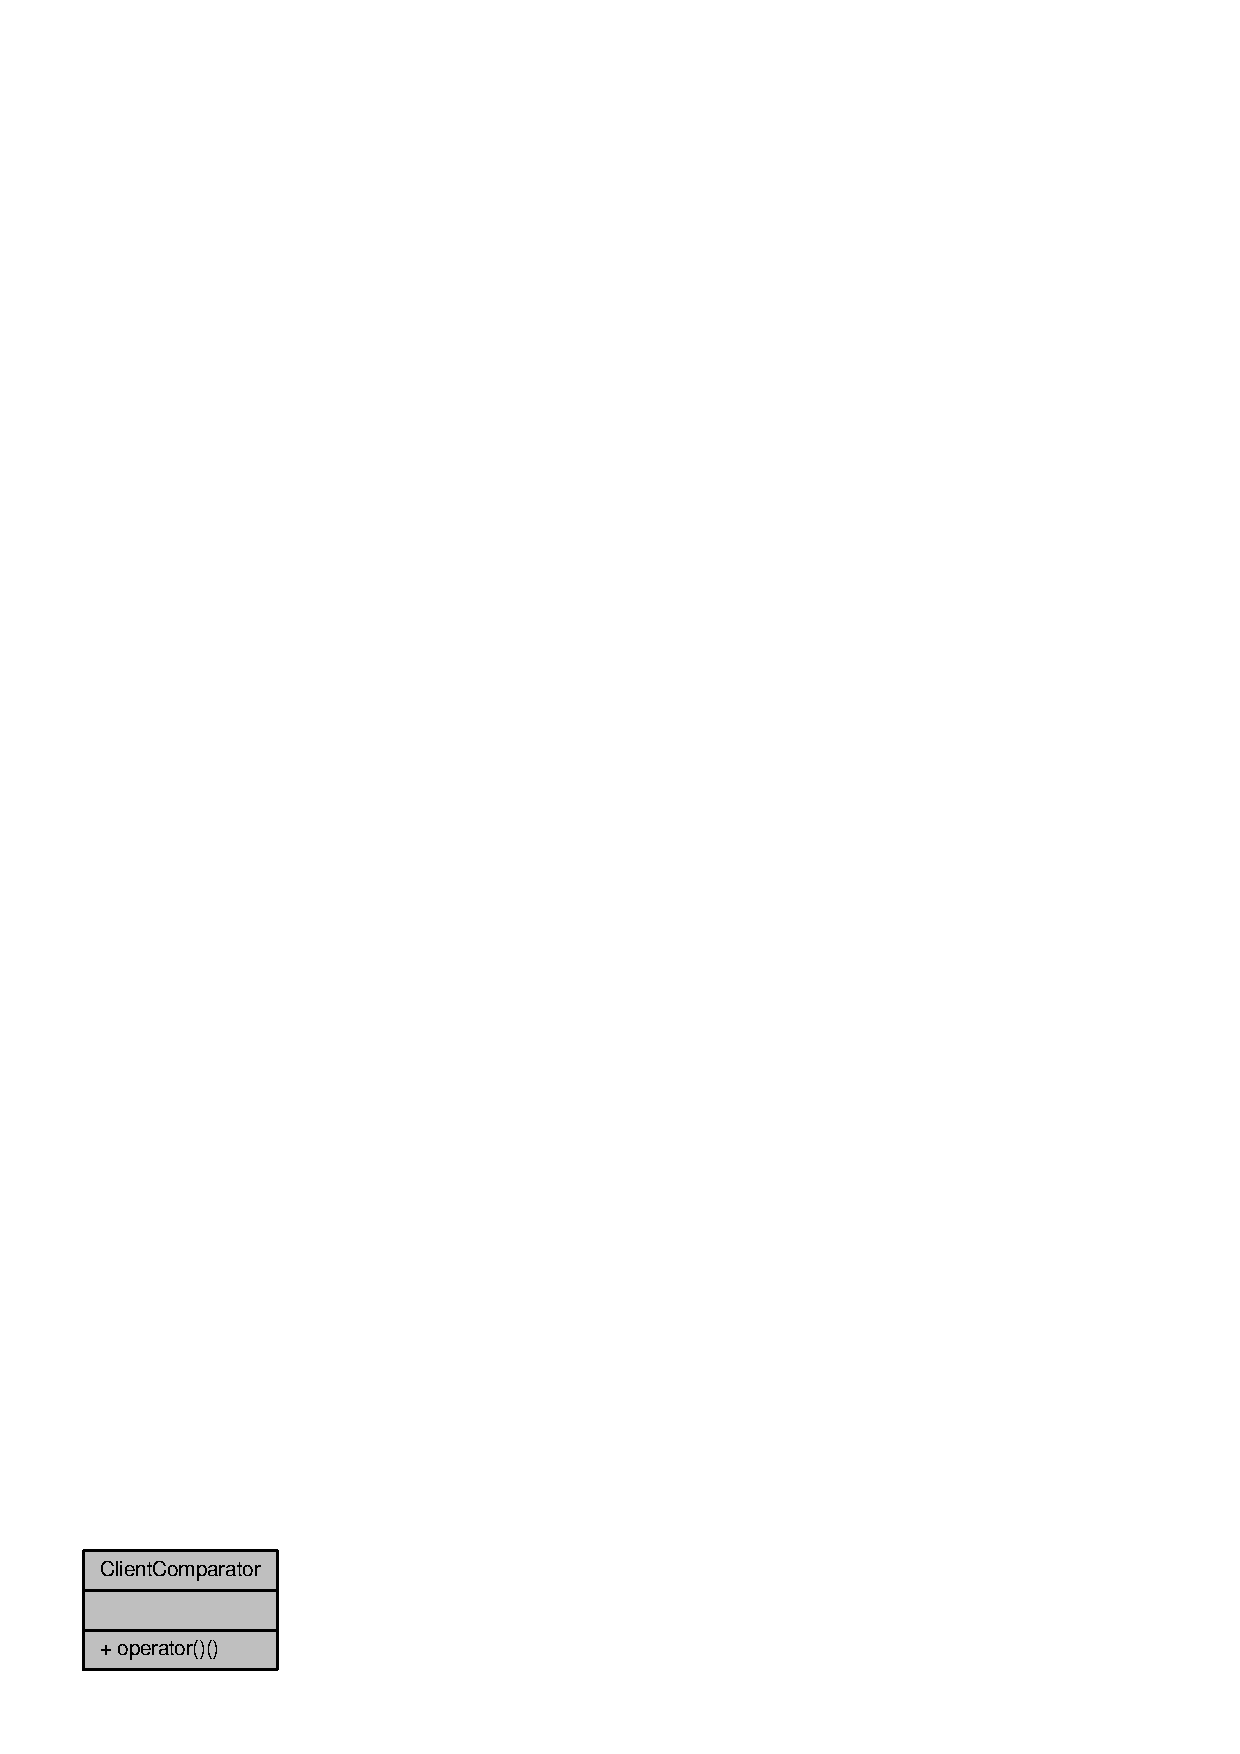
\includegraphics[width=137pt]{class_client_comparator__coll__graph}
\end{center}
\end{figure}
\subsection*{Public Member Functions}
\begin{DoxyCompactItemize}
\item 
bool {\bf operator()} (std\+::shared\+\_\+ptr$<$ const {\bf Client} $>$ lhs, std\+::shared\+\_\+ptr$<$ const {\bf Client} $>$ rhs) const 
\end{DoxyCompactItemize}


\subsection{Detailed Description}


Definition at line 13 of file Planning\+Scheduler.\+h.



\subsection{Member Function Documentation}
\index{Client\+Comparator@{Client\+Comparator}!operator()@{operator()}}
\index{operator()@{operator()}!Client\+Comparator@{Client\+Comparator}}
\subsubsection[{operator()}]{\setlength{\rightskip}{0pt plus 5cm}bool Client\+Comparator\+::operator() (
\begin{DoxyParamCaption}
\item[{std\+::shared\+\_\+ptr$<$ const {\bf Client} $>$}]{lhs, }
\item[{std\+::shared\+\_\+ptr$<$ const {\bf Client} $>$}]{rhs}
\end{DoxyParamCaption}
) const\hspace{0.3cm}{\ttfamily [inline]}}\label{class_client_comparator_a4b1c4c3f439964f9c417e744171e9956}


Definition at line 15 of file Planning\+Scheduler.\+h.



The documentation for this class was generated from the following file\+:\begin{DoxyCompactItemize}
\item 
include/{\bf Planning\+Scheduler.\+h}\end{DoxyCompactItemize}

\hypertarget{class_clock}{}\section{Clock Class Reference}
\label{class_clock}\index{Clock@{Clock}}


{\ttfamily \#include $<$Clock.\+h$>$}



Inheritance diagram for Clock\+:
\nopagebreak
\begin{figure}[H]
\begin{center}
\leavevmode
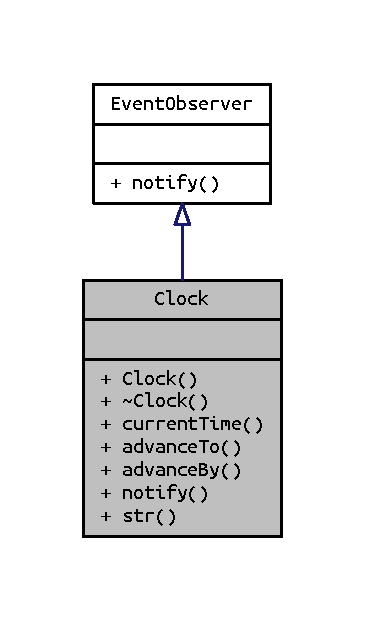
\includegraphics[width=175pt]{class_clock__inherit__graph}
\end{center}
\end{figure}


Collaboration diagram for Clock\+:
\nopagebreak
\begin{figure}[H]
\begin{center}
\leavevmode
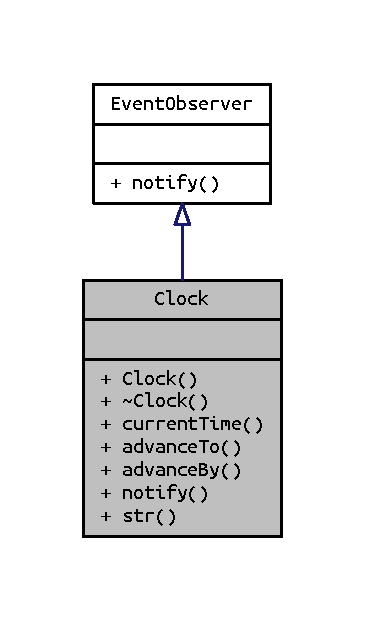
\includegraphics[width=175pt]{class_clock__coll__graph}
\end{center}
\end{figure}
\subsection*{Public Member Functions}
\begin{DoxyCompactItemize}
\item 
\hyperlink{class_clock_adbc370eb6b5f8d01645cf440188160a8}{Clock} ()
\item 
virtual \hyperlink{class_clock_afc976ce68fa85e15cc06f9ed47bddb7c}{$\sim$\+Clock} ()
\item 
unsigned long \hyperlink{class_clock_acfef0b6f07a1d424d2d6679a5ae8e612}{current\+Time} () const 
\item 
void \hyperlink{class_clock_a5970e64721aa434ab917f63c6466f3e8}{advance\+To} (const unsigned long time)
\item 
void \hyperlink{class_clock_a3e0c484fc257b6c7818614dc46dfd262}{advance\+By} (const unsigned long amount)
\item 
void \hyperlink{class_clock_a534758881637b06f765a24af22f9e8a1}{notify} (const std\+::shared\+\_\+ptr$<$ const \hyperlink{class_event}{Event} $>$ event)
\item 
std\+::string \hyperlink{class_clock_a21bdc10618f141f620227e81b23b2acf}{str} () const 
\end{DoxyCompactItemize}


\subsection{Constructor \& Destructor Documentation}
\hypertarget{class_clock_adbc370eb6b5f8d01645cf440188160a8}{}\index{Clock@{Clock}!Clock@{Clock}}
\index{Clock@{Clock}!Clock@{Clock}}
\subsubsection[{Clock}]{\setlength{\rightskip}{0pt plus 5cm}Clock\+::\+Clock (
\begin{DoxyParamCaption}
{}
\end{DoxyParamCaption}
)}\label{class_clock_adbc370eb6b5f8d01645cf440188160a8}
\hypertarget{class_clock_afc976ce68fa85e15cc06f9ed47bddb7c}{}\index{Clock@{Clock}!````~Clock@{$\sim$\+Clock}}
\index{````~Clock@{$\sim$\+Clock}!Clock@{Clock}}
\subsubsection[{$\sim$\+Clock}]{\setlength{\rightskip}{0pt plus 5cm}Clock\+::$\sim$\+Clock (
\begin{DoxyParamCaption}
{}
\end{DoxyParamCaption}
)\hspace{0.3cm}{\ttfamily [virtual]}}\label{class_clock_afc976ce68fa85e15cc06f9ed47bddb7c}


\subsection{Member Function Documentation}
\hypertarget{class_clock_a3e0c484fc257b6c7818614dc46dfd262}{}\index{Clock@{Clock}!advance\+By@{advance\+By}}
\index{advance\+By@{advance\+By}!Clock@{Clock}}
\subsubsection[{advance\+By}]{\setlength{\rightskip}{0pt plus 5cm}void Clock\+::advance\+By (
\begin{DoxyParamCaption}
\item[{const unsigned long}]{amount}
\end{DoxyParamCaption}
)}\label{class_clock_a3e0c484fc257b6c7818614dc46dfd262}
\hypertarget{class_clock_a5970e64721aa434ab917f63c6466f3e8}{}\index{Clock@{Clock}!advance\+To@{advance\+To}}
\index{advance\+To@{advance\+To}!Clock@{Clock}}
\subsubsection[{advance\+To}]{\setlength{\rightskip}{0pt plus 5cm}void Clock\+::advance\+To (
\begin{DoxyParamCaption}
\item[{const unsigned long}]{time}
\end{DoxyParamCaption}
)}\label{class_clock_a5970e64721aa434ab917f63c6466f3e8}


Here is the caller graph for this function\+:
\nopagebreak
\begin{figure}[H]
\begin{center}
\leavevmode
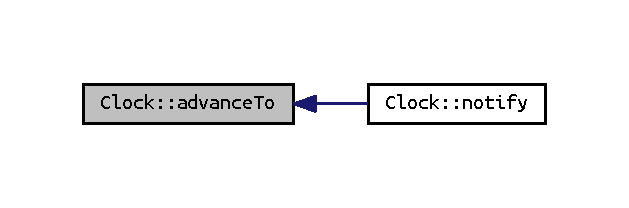
\includegraphics[width=302pt]{class_clock_a5970e64721aa434ab917f63c6466f3e8_icgraph}
\end{center}
\end{figure}


\hypertarget{class_clock_acfef0b6f07a1d424d2d6679a5ae8e612}{}\index{Clock@{Clock}!current\+Time@{current\+Time}}
\index{current\+Time@{current\+Time}!Clock@{Clock}}
\subsubsection[{current\+Time}]{\setlength{\rightskip}{0pt plus 5cm}unsigned long Clock\+::current\+Time (
\begin{DoxyParamCaption}
{}
\end{DoxyParamCaption}
) const}\label{class_clock_acfef0b6f07a1d424d2d6679a5ae8e612}
\hypertarget{class_clock_a534758881637b06f765a24af22f9e8a1}{}\index{Clock@{Clock}!notify@{notify}}
\index{notify@{notify}!Clock@{Clock}}
\subsubsection[{notify}]{\setlength{\rightskip}{0pt plus 5cm}void Clock\+::notify (
\begin{DoxyParamCaption}
\item[{const std\+::shared\+\_\+ptr$<$ const {\bf Event} $>$}]{event}
\end{DoxyParamCaption}
)\hspace{0.3cm}{\ttfamily [virtual]}}\label{class_clock_a534758881637b06f765a24af22f9e8a1}


Implements \hyperlink{class_event_observer_a81b3c545084ba3c8eaa8c83f5a0a4eb8}{Event\+Observer}.



Here is the call graph for this function\+:
\nopagebreak
\begin{figure}[H]
\begin{center}
\leavevmode
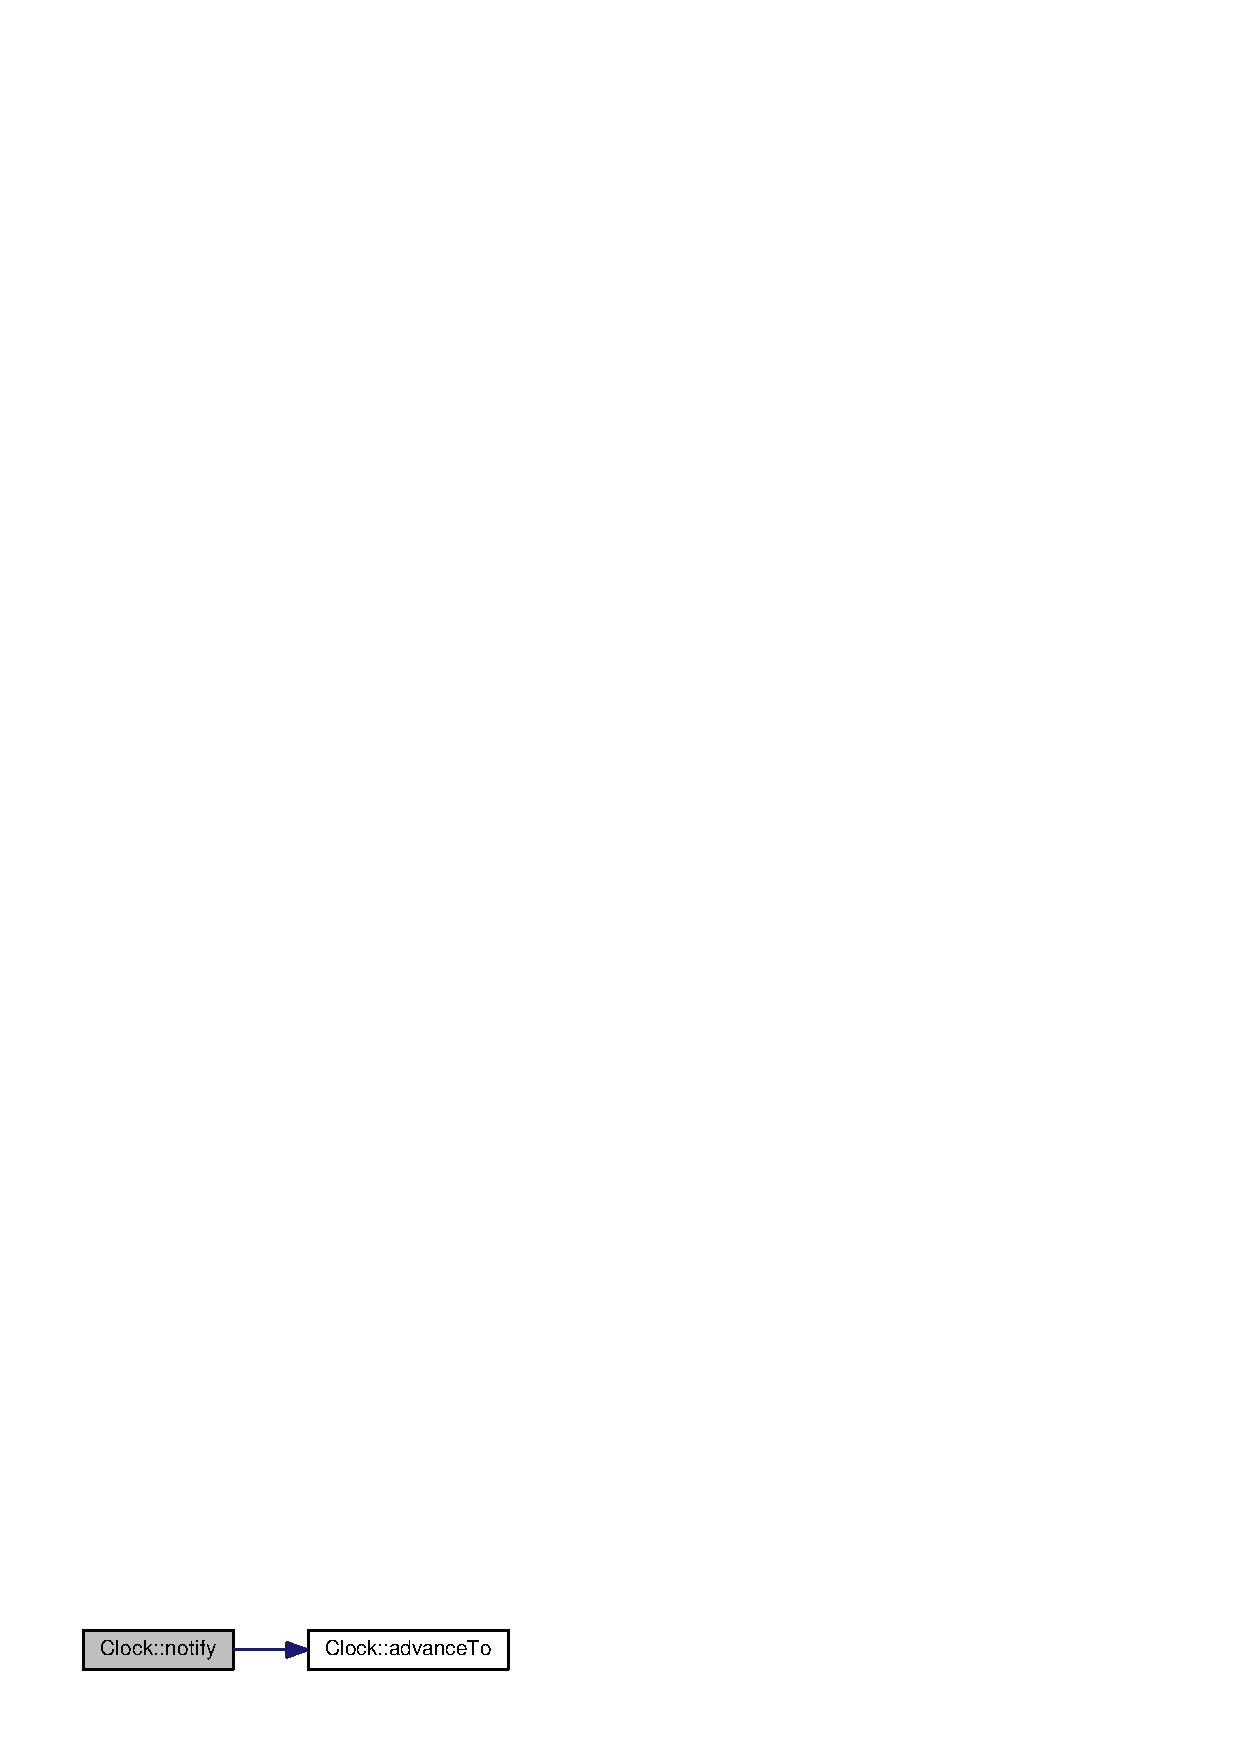
\includegraphics[width=302pt]{class_clock_a534758881637b06f765a24af22f9e8a1_cgraph}
\end{center}
\end{figure}


\hypertarget{class_clock_a21bdc10618f141f620227e81b23b2acf}{}\index{Clock@{Clock}!str@{str}}
\index{str@{str}!Clock@{Clock}}
\subsubsection[{str}]{\setlength{\rightskip}{0pt plus 5cm}std\+::string Clock\+::str (
\begin{DoxyParamCaption}
{}
\end{DoxyParamCaption}
) const}\label{class_clock_a21bdc10618f141f620227e81b23b2acf}


The documentation for this class was generated from the following files\+:\begin{DoxyCompactItemize}
\item 
include/\hyperlink{_clock_8h}{Clock.\+h}\item 
src/\hyperlink{_clock_8cpp}{Clock.\+cpp}\end{DoxyCompactItemize}

\section{Cost\+Function Class Reference}
\label{class_cost_function}\index{Cost\+Function@{Cost\+Function}}


{\ttfamily \#include $<$Cost\+Function.\+h$>$}



Inheritance diagram for Cost\+Function\+:\nopagebreak
\begin{figure}[H]
\begin{center}
\leavevmode
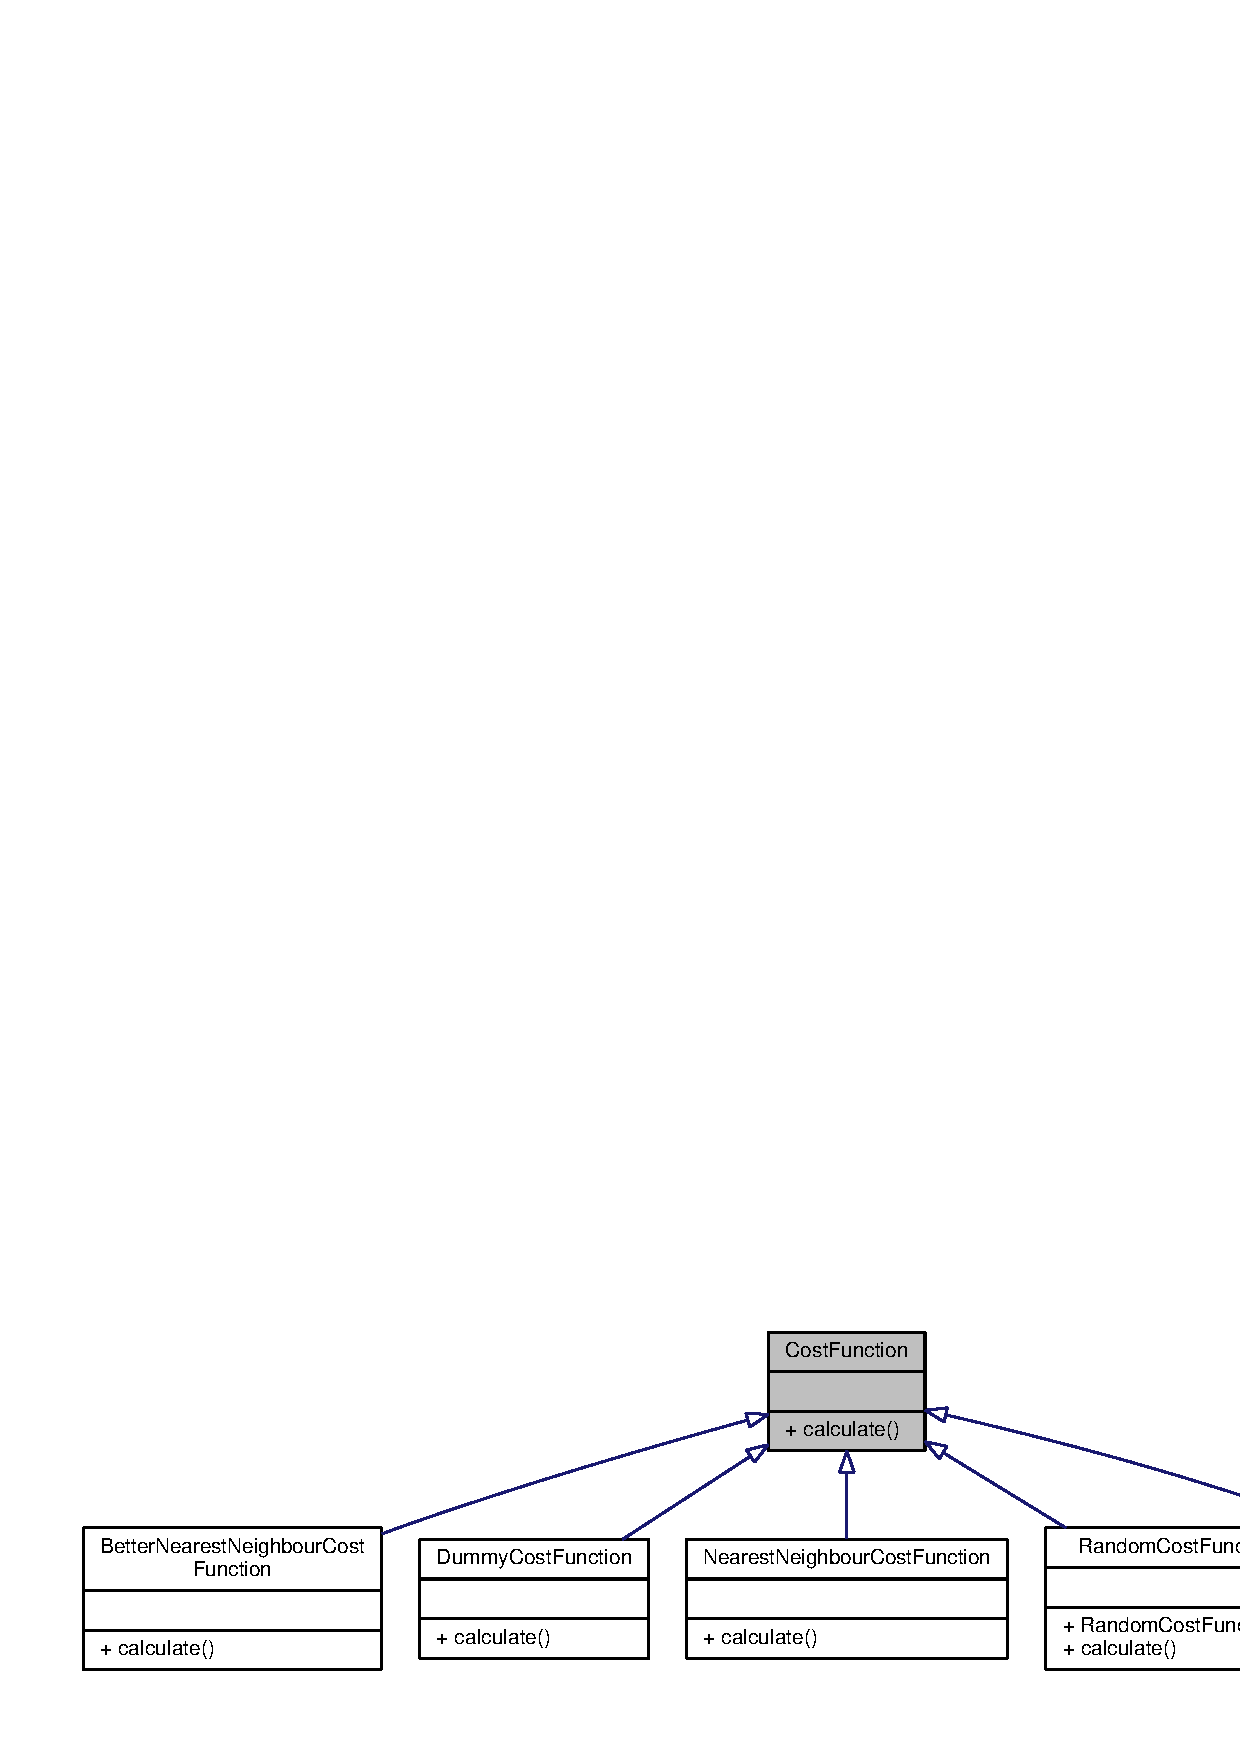
\includegraphics[width=350pt]{class_cost_function__inherit__graph}
\end{center}
\end{figure}


Collaboration diagram for Cost\+Function\+:\nopagebreak
\begin{figure}[H]
\begin{center}
\leavevmode
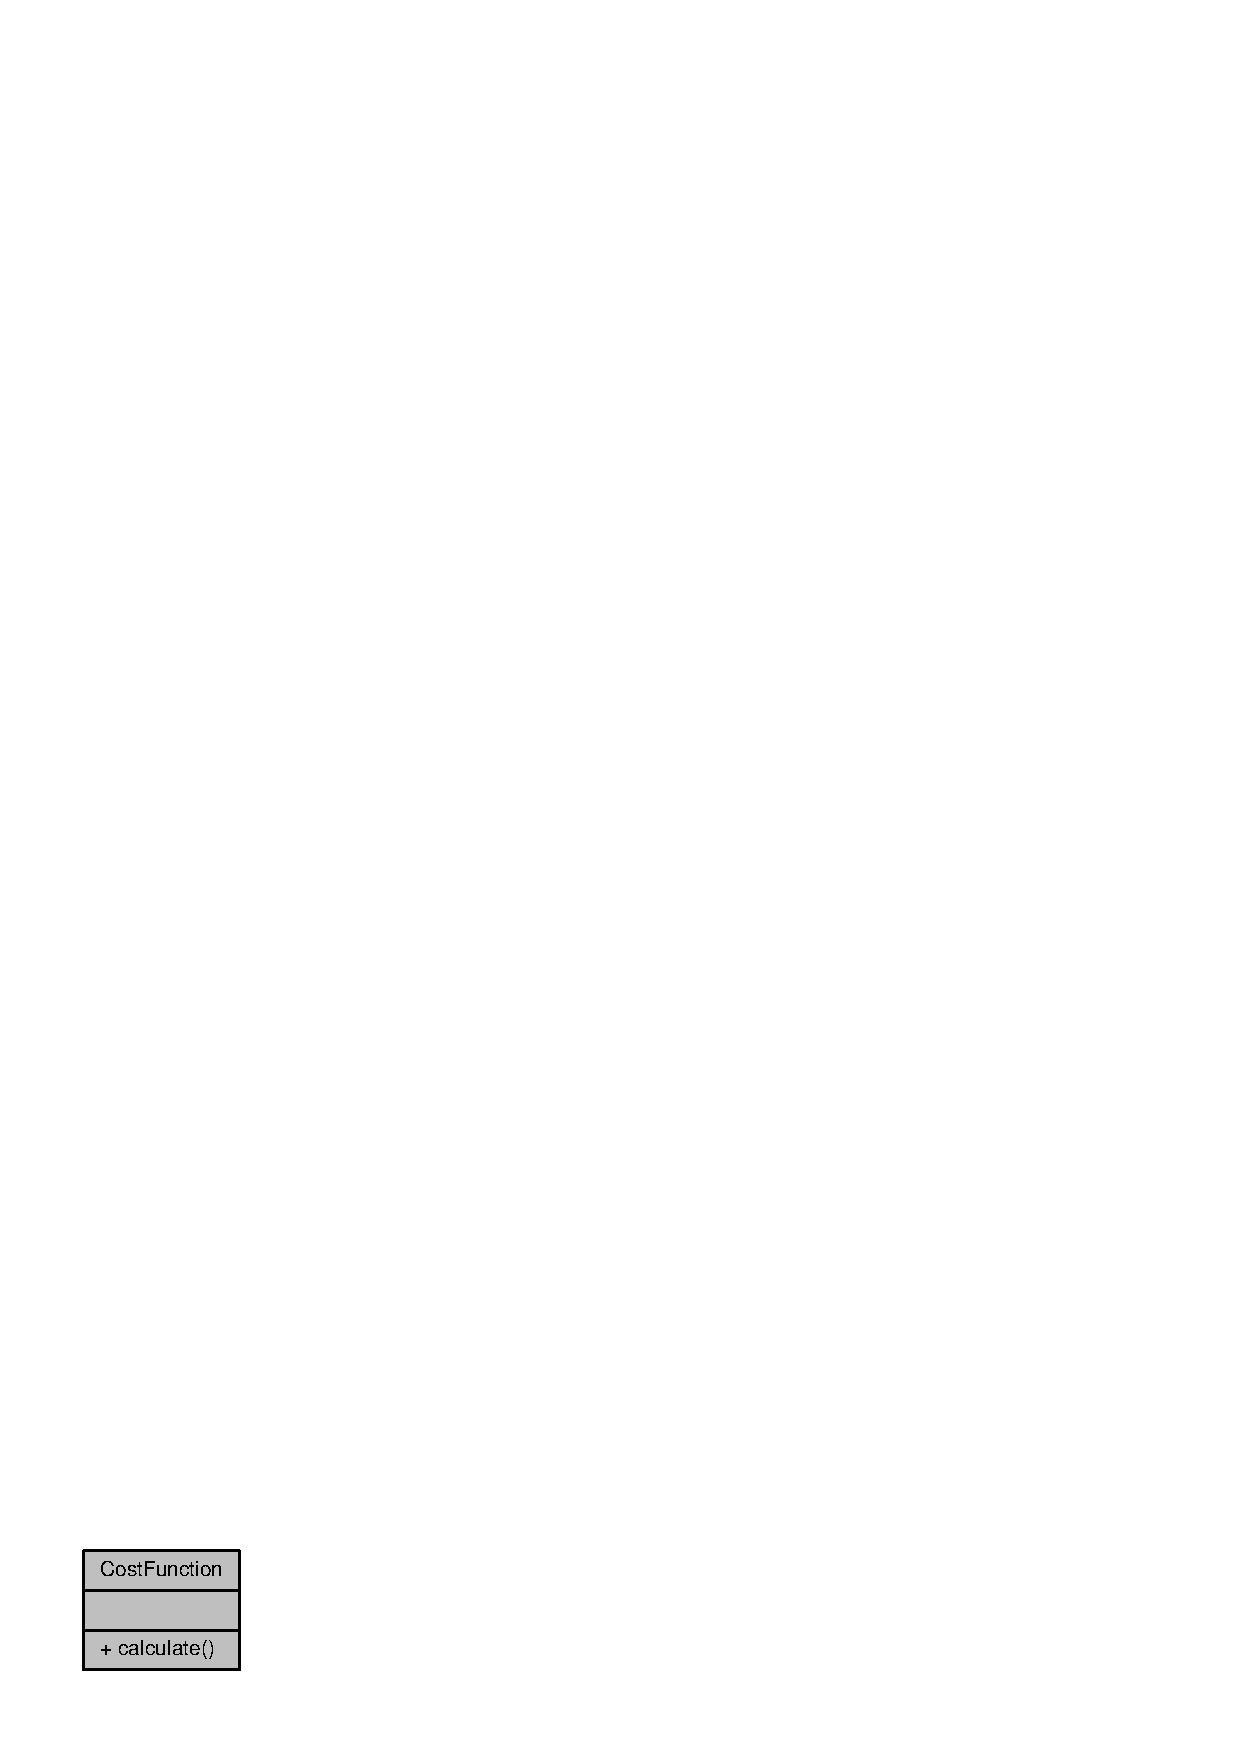
\includegraphics[width=119pt]{class_cost_function__coll__graph}
\end{center}
\end{figure}
\subsection*{Public Member Functions}
\begin{DoxyCompactItemize}
\item 
virtual float {\bf calculate} (const std\+::shared\+\_\+ptr$<$ const {\bf Building} $>$ building, const std\+::shared\+\_\+ptr$<$ const {\bf Elevator} $>$ elevator, const std\+::shared\+\_\+ptr$<$ const {\bf Client} $>$ client)=0
\end{DoxyCompactItemize}


\subsection{Detailed Description}


Definition at line 9 of file Cost\+Function.\+h.



\subsection{Member Function Documentation}
\index{Cost\+Function@{Cost\+Function}!calculate@{calculate}}
\index{calculate@{calculate}!Cost\+Function@{Cost\+Function}}
\subsubsection[{calculate}]{\setlength{\rightskip}{0pt plus 5cm}virtual float Cost\+Function\+::calculate (
\begin{DoxyParamCaption}
\item[{const std\+::shared\+\_\+ptr$<$ const {\bf Building} $>$}]{building, }
\item[{const std\+::shared\+\_\+ptr$<$ const {\bf Elevator} $>$}]{elevator, }
\item[{const std\+::shared\+\_\+ptr$<$ const {\bf Client} $>$}]{client}
\end{DoxyParamCaption}
)\hspace{0.3cm}{\ttfamily [pure virtual]}}\label{class_cost_function_ada1a1003e80f4f0e57b20d9a1e6a51c6}


Implemented in {\bf Random\+Cost\+Function} \doxyref{}{p.}{class_random_cost_function_a19c472a58df16e9805af2dfba3462fd9}, {\bf Better\+Nearest\+Neighbour\+Cost\+Function} \doxyref{}{p.}{class_better_nearest_neighbour_cost_function_a425ff56890dfc52fc4e0c28d8e9de5d5}, {\bf Dummy\+Cost\+Function} \doxyref{}{p.}{class_dummy_cost_function_a450e225a5a2d6bcab850255b2033c7bf}, {\bf Nearest\+Neighbour\+Cost\+Function} \doxyref{}{p.}{class_nearest_neighbour_cost_function_ab96d06d3bcd0f3cc56da5928d014c40e}, and {\bf Weighted\+Cost\+Function} \doxyref{}{p.}{class_weighted_cost_function_a6125501ba57f480e65de1b7c3bfdea39}.



The documentation for this class was generated from the following file\+:\begin{DoxyCompactItemize}
\item 
include/{\bf Cost\+Function.\+h}\end{DoxyCompactItemize}

\section{Cost\+Function\+Creator Class Reference}
\label{class_cost_function_creator}\index{Cost\+Function\+Creator@{Cost\+Function\+Creator}}


{\ttfamily \#include $<$Cost\+Function\+Creator.\+h$>$}



Collaboration diagram for Cost\+Function\+Creator\+:\nopagebreak
\begin{figure}[H]
\begin{center}
\leavevmode
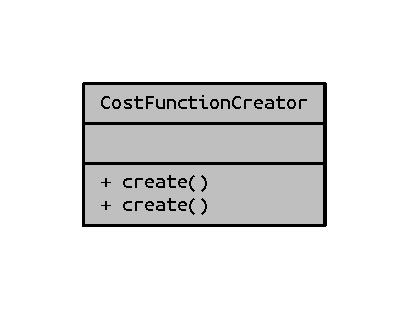
\includegraphics[width=151pt]{class_cost_function_creator__coll__graph}
\end{center}
\end{figure}
\subsection*{Static Public Member Functions}
\begin{DoxyCompactItemize}
\item 
{\footnotesize template$<$class T $>$ }\\static const std\+::shared\+\_\+ptr$<$ {\bf Cost\+Function} $>$ {\bf create} ()
\item 
static const std\+::shared\+\_\+ptr$<$ {\bf Cost\+Function} $>$ {\bf create} (const {\bf Cost\+Function\+Type} cost\+Function\+Type)
\end{DoxyCompactItemize}


\subsection{Detailed Description}


Definition at line 12 of file Cost\+Function\+Creator.\+h.



\subsection{Member Function Documentation}
\index{Cost\+Function\+Creator@{Cost\+Function\+Creator}!create@{create}}
\index{create@{create}!Cost\+Function\+Creator@{Cost\+Function\+Creator}}
\subsubsection[{create}]{\setlength{\rightskip}{0pt plus 5cm}template$<$class T $>$ const std\+::shared\+\_\+ptr$<$ {\bf Cost\+Function} $>$ Cost\+Function\+Creator\+::create (
\begin{DoxyParamCaption}
{}
\end{DoxyParamCaption}
)\hspace{0.3cm}{\ttfamily [static]}}\label{class_cost_function_creator_a2f73ed3b5e34c2cfa891849ab62adda5}


Definition at line 19 of file Cost\+Function\+Creator.\+h.



Here is the caller graph for this function\+:\nopagebreak
\begin{figure}[H]
\begin{center}
\leavevmode
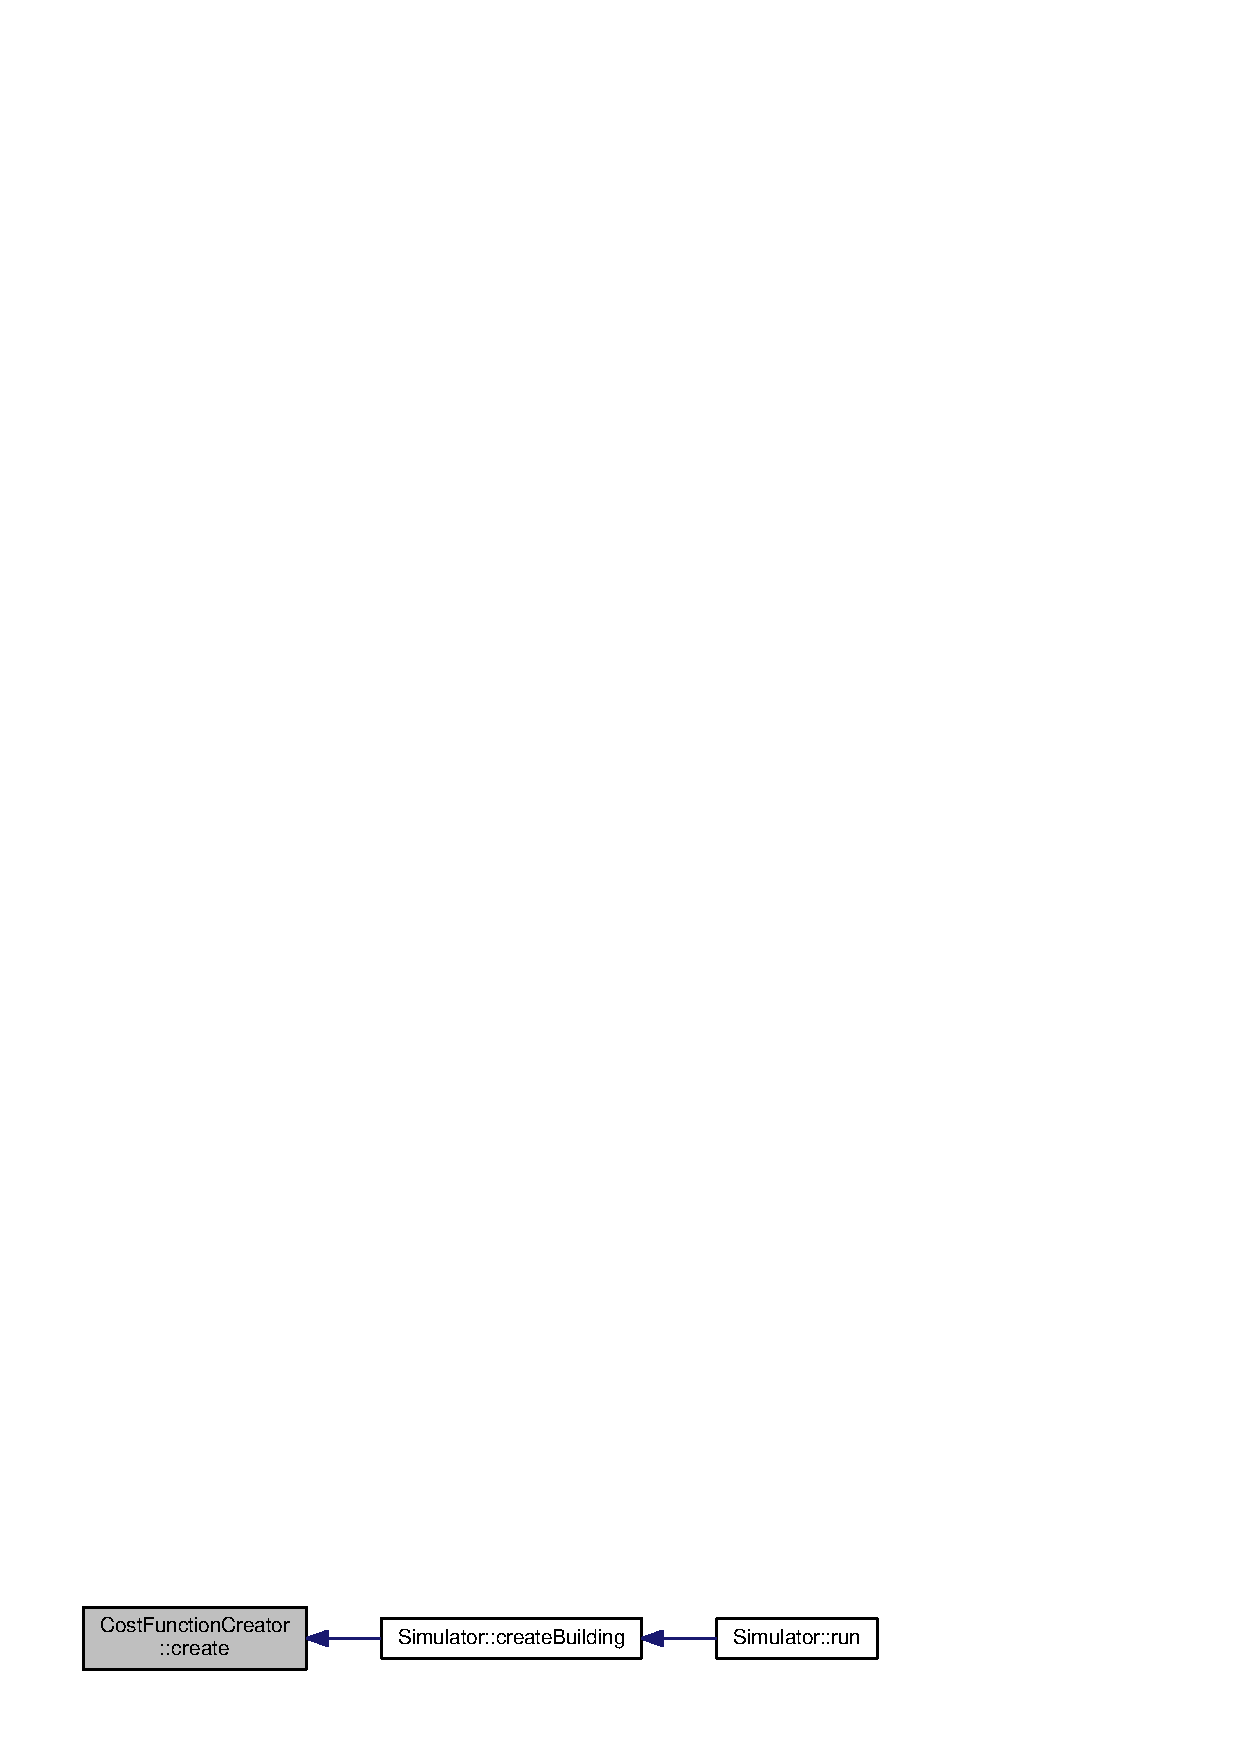
\includegraphics[width=350pt]{class_cost_function_creator_a2f73ed3b5e34c2cfa891849ab62adda5_icgraph}
\end{center}
\end{figure}


\index{Cost\+Function\+Creator@{Cost\+Function\+Creator}!create@{create}}
\index{create@{create}!Cost\+Function\+Creator@{Cost\+Function\+Creator}}
\subsubsection[{create}]{\setlength{\rightskip}{0pt plus 5cm}const std\+::shared\+\_\+ptr$<$ {\bf Cost\+Function} $>$ Cost\+Function\+Creator\+::create (
\begin{DoxyParamCaption}
\item[{const {\bf Cost\+Function\+Type}}]{cost\+Function\+Type}
\end{DoxyParamCaption}
)\hspace{0.3cm}{\ttfamily [static]}}\label{class_cost_function_creator_a69479ceb186c544fd9a800791be7dbe9}


Definition at line 24 of file Cost\+Function\+Creator.\+h.



The documentation for this class was generated from the following file\+:\begin{DoxyCompactItemize}
\item 
include/{\bf Cost\+Function\+Creator.\+h}\end{DoxyCompactItemize}

\hypertarget{class_elevator}{}\section{Elevator Class Reference}
\label{class_elevator}\index{Elevator@{Elevator}}


{\ttfamily \#include $<$Elevator.\+h$>$}



Inheritance diagram for Elevator\+:
\nopagebreak
\begin{figure}[H]
\begin{center}
\leavevmode
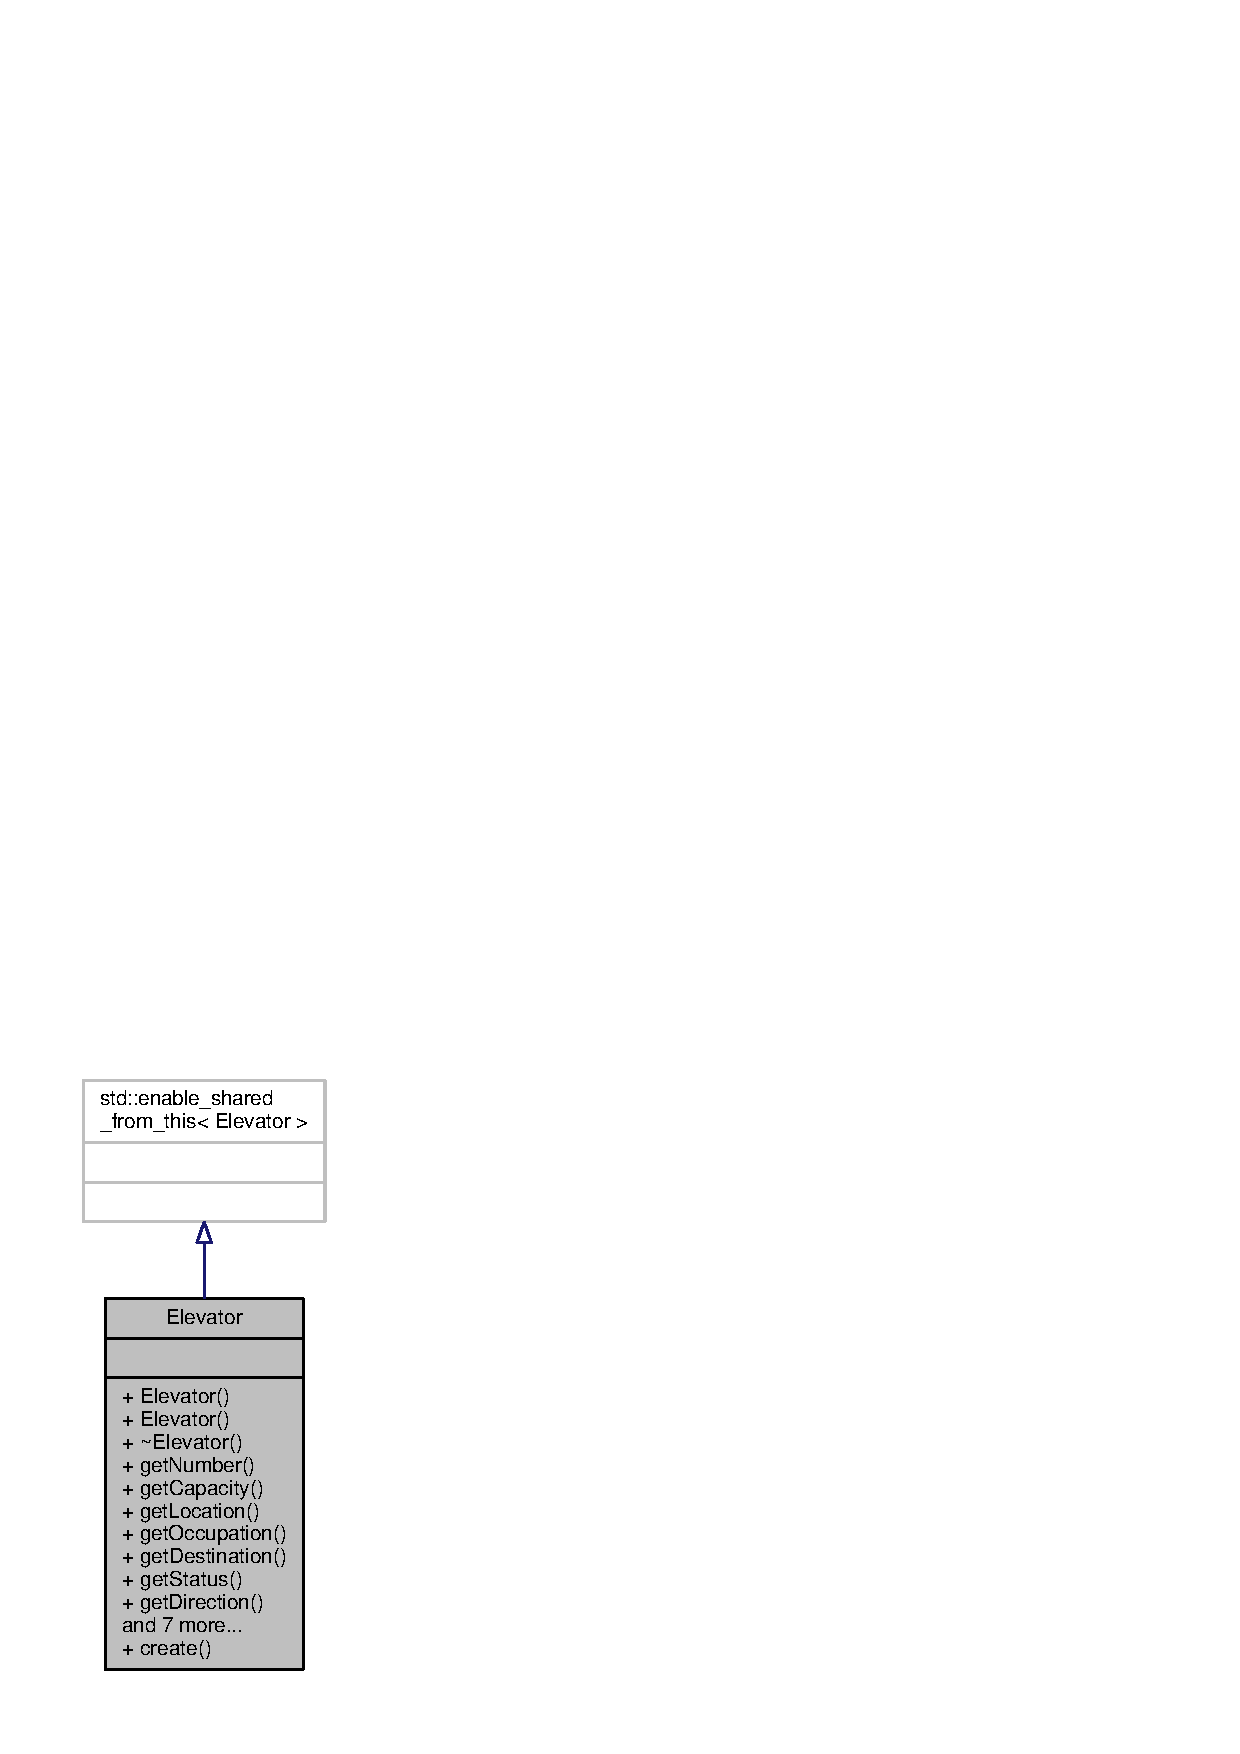
\includegraphics[width=280pt]{class_elevator__inherit__graph}
\end{center}
\end{figure}


Collaboration diagram for Elevator\+:
\nopagebreak
\begin{figure}[H]
\begin{center}
\leavevmode
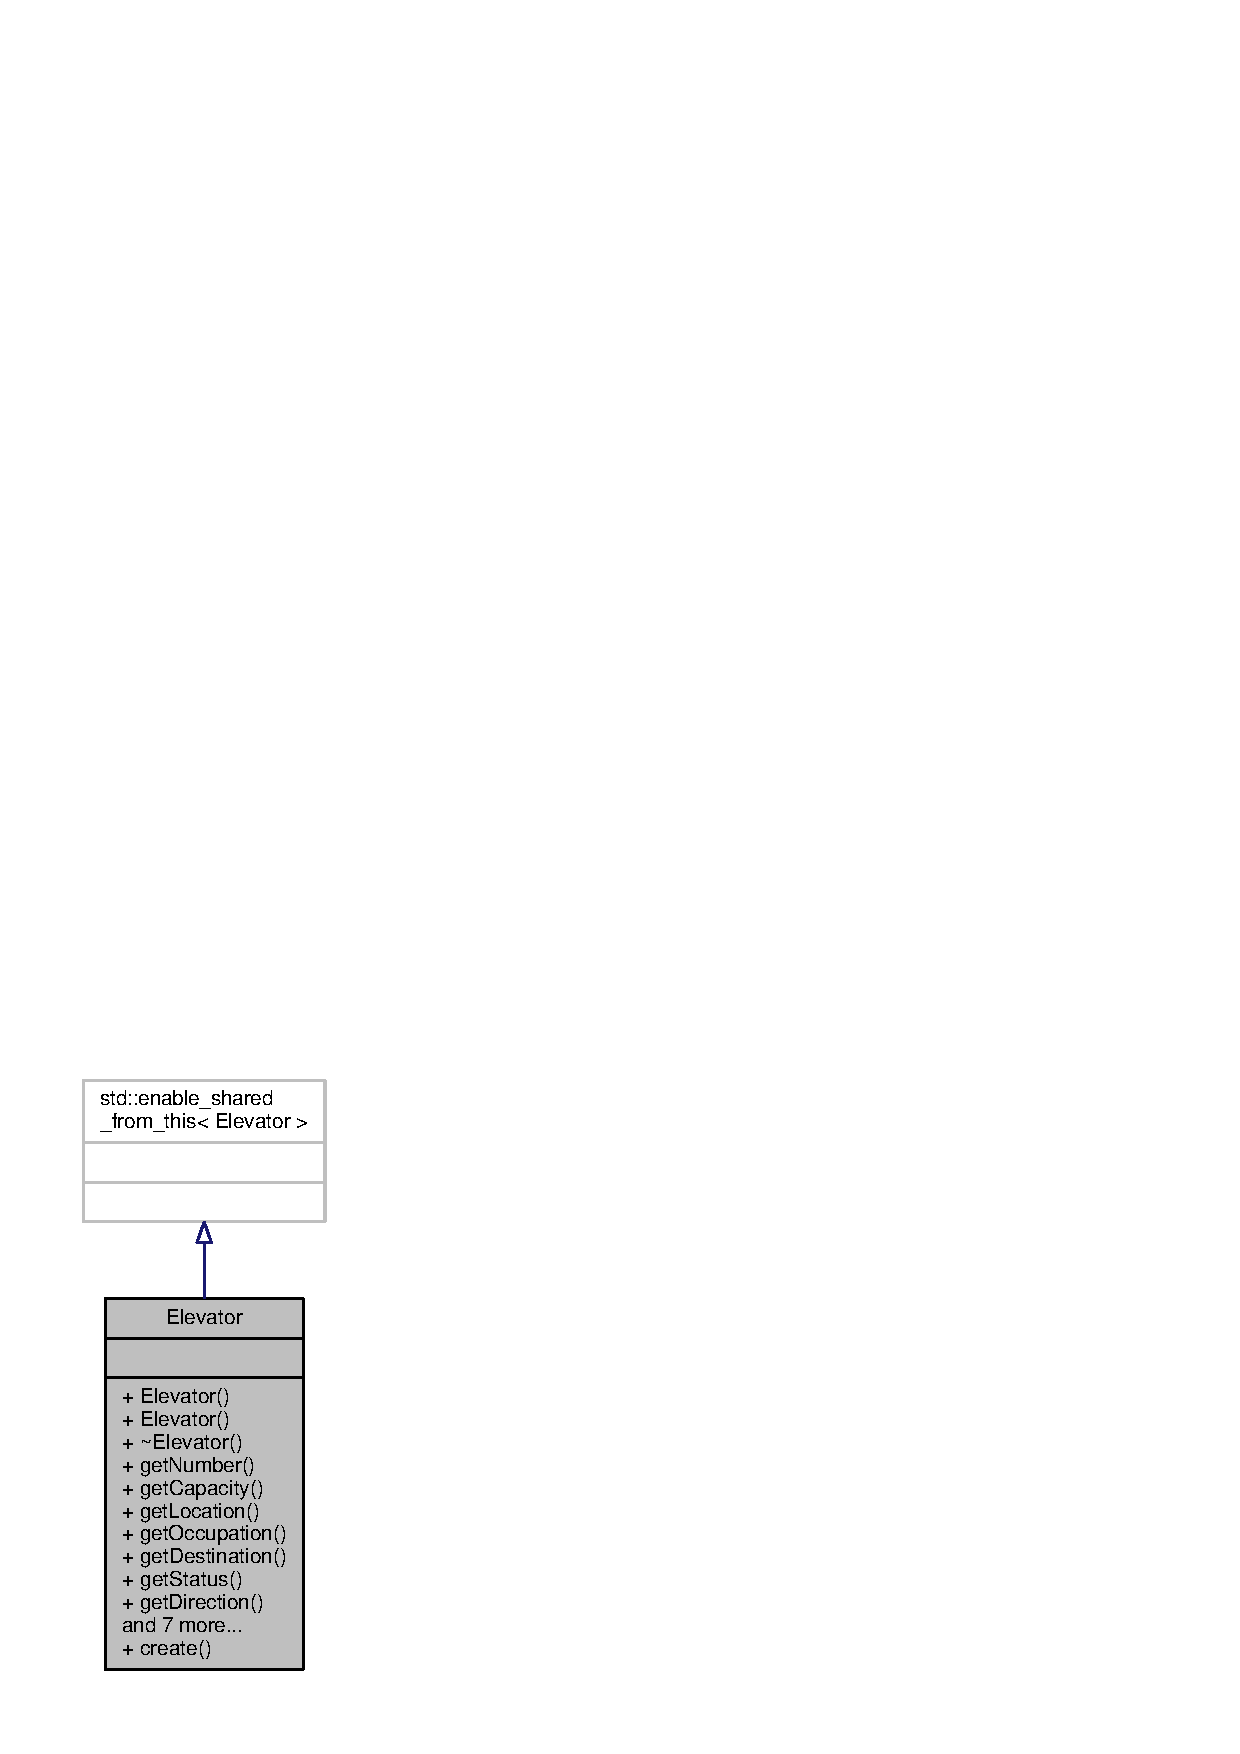
\includegraphics[width=280pt]{class_elevator__coll__graph}
\end{center}
\end{figure}
\subsection*{Public Member Functions}
\begin{DoxyCompactItemize}
\item 
\hyperlink{class_elevator_a43c3de38489fb58f17fc60e91bd522e7}{Elevator} (int number, int capacity, int floor)
\item 
virtual \hyperlink{class_elevator_a6e2fb71cfcde094c087b8a19a8bcab4b}{$\sim$\+Elevator} ()
\item 
int \hyperlink{class_elevator_a8e21ac6a7a3923ab2fd41b6d4b8295ba}{get\+Number} () const 
\item 
int \hyperlink{class_elevator_ab1a532d6b4df19b77e7a8ce4727e6d74}{get\+Capacity} () const 
\item 
int \hyperlink{class_elevator_a6b50953b97442601165a3fe656d76776}{get\+Location} () const 
\item 
float \hyperlink{class_elevator_a2189014eaa1af1a32eb6d12c13b820ff}{get\+Occupation} () const 
\item 
std\+::pair$<$ int, \hyperlink{_direction_8h_a224b9163917ac32fc95a60d8c1eec3aa}{Direction} $>$ \hyperlink{class_elevator_ad8cb66c8d7bdd3e82faf25e702bbc024}{get\+Destination} () const 
\item 
\hyperlink{_status_8h_a67a0db04d321a74b7e7fcfd3f1a3f70b}{Status} \hyperlink{class_elevator_a53345cce9f31247b8b85cba2cac91922}{get\+Status} () const 
\item 
\hyperlink{_direction_8h_a224b9163917ac32fc95a60d8c1eec3aa}{Direction} \hyperlink{class_elevator_a658315b18e536447f56a68220e35f45b}{get\+Direction} () const 
\item 
const std\+::shared\+\_\+ptr$<$ const std\+::vector$<$ std\+::shared\+\_\+ptr$<$ \hyperlink{class_client}{Client} $>$ $>$ $>$ \hyperlink{class_elevator_ad12bd410a7c6068b3653d4756cdad7c3}{get\+Passengers} () const 
\item 
void \hyperlink{class_elevator_ae5dbc53a35f77c0a8715b3e0f4b7d304}{set\+Destination} (std\+::pair$<$ int, \hyperlink{_direction_8h_a224b9163917ac32fc95a60d8c1eec3aa}{Direction} $>$ destination)
\item 
bool \hyperlink{class_elevator_aca22adae98cf171ac842c721dbb25248}{can\+Enter} (std\+::shared\+\_\+ptr$<$ const \hyperlink{class_client}{Client} $>$ client) const 
\item 
void \hyperlink{class_elevator_a79725eb058974b68669b717d956ddadd}{add\+Passenger} (std\+::shared\+\_\+ptr$<$ \hyperlink{class_client}{Client} $>$ client)
\item 
void \hyperlink{class_elevator_aebc0dff2d1966a4ea336a159b95bdf05}{move} ()
\item 
std\+::shared\+\_\+ptr$<$ std\+::vector$<$ std\+::shared\+\_\+ptr$<$ \hyperlink{class_client}{Client} $>$ $>$ $>$ \hyperlink{class_elevator_aa729c45a7dc7828f9bf4e30bbeb7ed83}{drop\+Passengers\+To\+Current\+Location} ()
\end{DoxyCompactItemize}
\subsection*{Static Public Member Functions}
\begin{DoxyCompactItemize}
\item 
static std\+::shared\+\_\+ptr$<$ std\+::vector$<$ std\+::shared\+\_\+ptr$<$ \hyperlink{class_elevator}{Elevator} $>$ $>$ $>$ \hyperlink{class_elevator_a6a5d8cb3159ee98e343042df0ff7f2ba}{create} (const std\+::shared\+\_\+ptr$<$ const \hyperlink{class_simulator}{Simulator} $>$ simulator)
\end{DoxyCompactItemize}


\subsection{Constructor \& Destructor Documentation}
\hypertarget{class_elevator_a43c3de38489fb58f17fc60e91bd522e7}{}\index{Elevator@{Elevator}!Elevator@{Elevator}}
\index{Elevator@{Elevator}!Elevator@{Elevator}}
\subsubsection[{Elevator}]{\setlength{\rightskip}{0pt plus 5cm}Elevator\+::\+Elevator (
\begin{DoxyParamCaption}
\item[{int}]{number, }
\item[{int}]{capacity, }
\item[{int}]{floor}
\end{DoxyParamCaption}
)}\label{class_elevator_a43c3de38489fb58f17fc60e91bd522e7}
\hypertarget{class_elevator_a6e2fb71cfcde094c087b8a19a8bcab4b}{}\index{Elevator@{Elevator}!````~Elevator@{$\sim$\+Elevator}}
\index{````~Elevator@{$\sim$\+Elevator}!Elevator@{Elevator}}
\subsubsection[{$\sim$\+Elevator}]{\setlength{\rightskip}{0pt plus 5cm}Elevator\+::$\sim$\+Elevator (
\begin{DoxyParamCaption}
{}
\end{DoxyParamCaption}
)\hspace{0.3cm}{\ttfamily [virtual]}}\label{class_elevator_a6e2fb71cfcde094c087b8a19a8bcab4b}


\subsection{Member Function Documentation}
\hypertarget{class_elevator_a79725eb058974b68669b717d956ddadd}{}\index{Elevator@{Elevator}!add\+Passenger@{add\+Passenger}}
\index{add\+Passenger@{add\+Passenger}!Elevator@{Elevator}}
\subsubsection[{add\+Passenger}]{\setlength{\rightskip}{0pt plus 5cm}void Elevator\+::add\+Passenger (
\begin{DoxyParamCaption}
\item[{std\+::shared\+\_\+ptr$<$ {\bf Client} $>$}]{client}
\end{DoxyParamCaption}
)}\label{class_elevator_a79725eb058974b68669b717d956ddadd}
\hypertarget{class_elevator_aca22adae98cf171ac842c721dbb25248}{}\index{Elevator@{Elevator}!can\+Enter@{can\+Enter}}
\index{can\+Enter@{can\+Enter}!Elevator@{Elevator}}
\subsubsection[{can\+Enter}]{\setlength{\rightskip}{0pt plus 5cm}bool Elevator\+::can\+Enter (
\begin{DoxyParamCaption}
\item[{std\+::shared\+\_\+ptr$<$ const {\bf Client} $>$}]{client}
\end{DoxyParamCaption}
) const}\label{class_elevator_aca22adae98cf171ac842c721dbb25248}
\hypertarget{class_elevator_a6a5d8cb3159ee98e343042df0ff7f2ba}{}\index{Elevator@{Elevator}!create@{create}}
\index{create@{create}!Elevator@{Elevator}}
\subsubsection[{create}]{\setlength{\rightskip}{0pt plus 5cm}std\+::shared\+\_\+ptr$<$ std\+::vector$<$ std\+::shared\+\_\+ptr$<$ {\bf Elevator} $>$ $>$ $>$ Elevator\+::create (
\begin{DoxyParamCaption}
\item[{const std\+::shared\+\_\+ptr$<$ const {\bf Simulator} $>$}]{simulator}
\end{DoxyParamCaption}
)\hspace{0.3cm}{\ttfamily [static]}}\label{class_elevator_a6a5d8cb3159ee98e343042df0ff7f2ba}


Here is the caller graph for this function\+:
\nopagebreak
\begin{figure}[H]
\begin{center}
\leavevmode
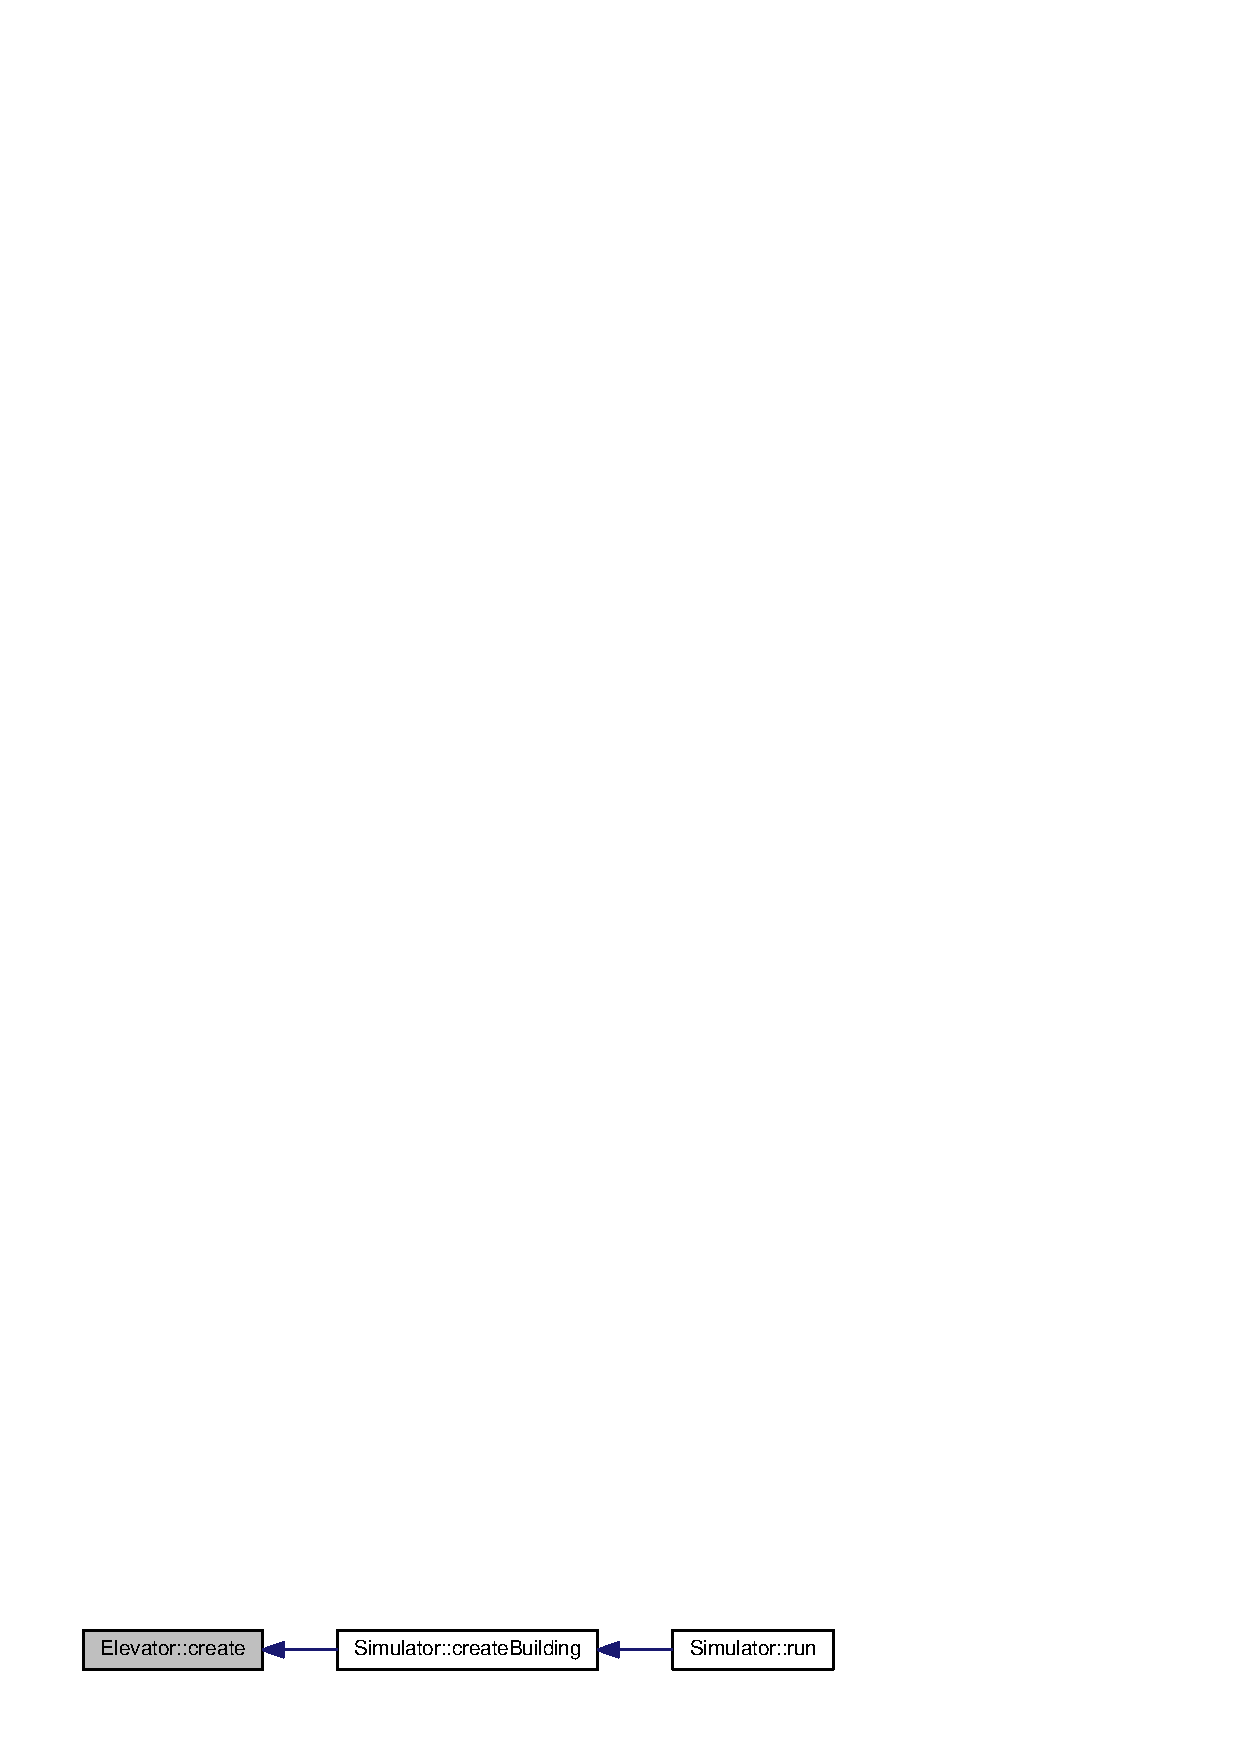
\includegraphics[width=350pt]{class_elevator_a6a5d8cb3159ee98e343042df0ff7f2ba_icgraph}
\end{center}
\end{figure}


\hypertarget{class_elevator_aa729c45a7dc7828f9bf4e30bbeb7ed83}{}\index{Elevator@{Elevator}!drop\+Passengers\+To\+Current\+Location@{drop\+Passengers\+To\+Current\+Location}}
\index{drop\+Passengers\+To\+Current\+Location@{drop\+Passengers\+To\+Current\+Location}!Elevator@{Elevator}}
\subsubsection[{drop\+Passengers\+To\+Current\+Location}]{\setlength{\rightskip}{0pt plus 5cm}std\+::shared\+\_\+ptr$<$ std\+::vector$<$ std\+::shared\+\_\+ptr$<$ {\bf Client} $>$ $>$ $>$ Elevator\+::drop\+Passengers\+To\+Current\+Location (
\begin{DoxyParamCaption}
{}
\end{DoxyParamCaption}
)}\label{class_elevator_aa729c45a7dc7828f9bf4e30bbeb7ed83}
\hypertarget{class_elevator_ab1a532d6b4df19b77e7a8ce4727e6d74}{}\index{Elevator@{Elevator}!get\+Capacity@{get\+Capacity}}
\index{get\+Capacity@{get\+Capacity}!Elevator@{Elevator}}
\subsubsection[{get\+Capacity}]{\setlength{\rightskip}{0pt plus 5cm}int Elevator\+::get\+Capacity (
\begin{DoxyParamCaption}
{}
\end{DoxyParamCaption}
) const}\label{class_elevator_ab1a532d6b4df19b77e7a8ce4727e6d74}
\hypertarget{class_elevator_ad8cb66c8d7bdd3e82faf25e702bbc024}{}\index{Elevator@{Elevator}!get\+Destination@{get\+Destination}}
\index{get\+Destination@{get\+Destination}!Elevator@{Elevator}}
\subsubsection[{get\+Destination}]{\setlength{\rightskip}{0pt plus 5cm}std\+::pair$<$ int, {\bf Direction} $>$ Elevator\+::get\+Destination (
\begin{DoxyParamCaption}
{}
\end{DoxyParamCaption}
) const}\label{class_elevator_ad8cb66c8d7bdd3e82faf25e702bbc024}
\hypertarget{class_elevator_a658315b18e536447f56a68220e35f45b}{}\index{Elevator@{Elevator}!get\+Direction@{get\+Direction}}
\index{get\+Direction@{get\+Direction}!Elevator@{Elevator}}
\subsubsection[{get\+Direction}]{\setlength{\rightskip}{0pt plus 5cm}{\bf Direction} Elevator\+::get\+Direction (
\begin{DoxyParamCaption}
{}
\end{DoxyParamCaption}
) const}\label{class_elevator_a658315b18e536447f56a68220e35f45b}
\hypertarget{class_elevator_a6b50953b97442601165a3fe656d76776}{}\index{Elevator@{Elevator}!get\+Location@{get\+Location}}
\index{get\+Location@{get\+Location}!Elevator@{Elevator}}
\subsubsection[{get\+Location}]{\setlength{\rightskip}{0pt plus 5cm}int Elevator\+::get\+Location (
\begin{DoxyParamCaption}
{}
\end{DoxyParamCaption}
) const}\label{class_elevator_a6b50953b97442601165a3fe656d76776}
\hypertarget{class_elevator_a8e21ac6a7a3923ab2fd41b6d4b8295ba}{}\index{Elevator@{Elevator}!get\+Number@{get\+Number}}
\index{get\+Number@{get\+Number}!Elevator@{Elevator}}
\subsubsection[{get\+Number}]{\setlength{\rightskip}{0pt plus 5cm}int Elevator\+::get\+Number (
\begin{DoxyParamCaption}
{}
\end{DoxyParamCaption}
) const}\label{class_elevator_a8e21ac6a7a3923ab2fd41b6d4b8295ba}
\hypertarget{class_elevator_a2189014eaa1af1a32eb6d12c13b820ff}{}\index{Elevator@{Elevator}!get\+Occupation@{get\+Occupation}}
\index{get\+Occupation@{get\+Occupation}!Elevator@{Elevator}}
\subsubsection[{get\+Occupation}]{\setlength{\rightskip}{0pt plus 5cm}float Elevator\+::get\+Occupation (
\begin{DoxyParamCaption}
{}
\end{DoxyParamCaption}
) const}\label{class_elevator_a2189014eaa1af1a32eb6d12c13b820ff}
\hypertarget{class_elevator_ad12bd410a7c6068b3653d4756cdad7c3}{}\index{Elevator@{Elevator}!get\+Passengers@{get\+Passengers}}
\index{get\+Passengers@{get\+Passengers}!Elevator@{Elevator}}
\subsubsection[{get\+Passengers}]{\setlength{\rightskip}{0pt plus 5cm}const std\+::shared\+\_\+ptr$<$ const std\+::vector$<$ std\+::shared\+\_\+ptr$<$ {\bf Client} $>$ $>$ $>$ Elevator\+::get\+Passengers (
\begin{DoxyParamCaption}
{}
\end{DoxyParamCaption}
) const}\label{class_elevator_ad12bd410a7c6068b3653d4756cdad7c3}
\hypertarget{class_elevator_a53345cce9f31247b8b85cba2cac91922}{}\index{Elevator@{Elevator}!get\+Status@{get\+Status}}
\index{get\+Status@{get\+Status}!Elevator@{Elevator}}
\subsubsection[{get\+Status}]{\setlength{\rightskip}{0pt plus 5cm}{\bf Status} Elevator\+::get\+Status (
\begin{DoxyParamCaption}
{}
\end{DoxyParamCaption}
) const}\label{class_elevator_a53345cce9f31247b8b85cba2cac91922}
\hypertarget{class_elevator_aebc0dff2d1966a4ea336a159b95bdf05}{}\index{Elevator@{Elevator}!move@{move}}
\index{move@{move}!Elevator@{Elevator}}
\subsubsection[{move}]{\setlength{\rightskip}{0pt plus 5cm}void Elevator\+::move (
\begin{DoxyParamCaption}
{}
\end{DoxyParamCaption}
)}\label{class_elevator_aebc0dff2d1966a4ea336a159b95bdf05}
\hypertarget{class_elevator_ae5dbc53a35f77c0a8715b3e0f4b7d304}{}\index{Elevator@{Elevator}!set\+Destination@{set\+Destination}}
\index{set\+Destination@{set\+Destination}!Elevator@{Elevator}}
\subsubsection[{set\+Destination}]{\setlength{\rightskip}{0pt plus 5cm}void Elevator\+::set\+Destination (
\begin{DoxyParamCaption}
\item[{std\+::pair$<$ int, {\bf Direction} $>$}]{destination}
\end{DoxyParamCaption}
)}\label{class_elevator_ae5dbc53a35f77c0a8715b3e0f4b7d304}


The documentation for this class was generated from the following files\+:\begin{DoxyCompactItemize}
\item 
include/\hyperlink{_elevator_8h}{Elevator.\+h}\item 
src/\hyperlink{_elevator_8cpp}{Elevator.\+cpp}\end{DoxyCompactItemize}

\section{Event Class Reference}
\label{class_event}\index{Event@{Event}}


{\ttfamily \#include $<$Event.\+h$>$}



Inheritance diagram for Event\+:
\nopagebreak
\begin{figure}[H]
\begin{center}
\leavevmode
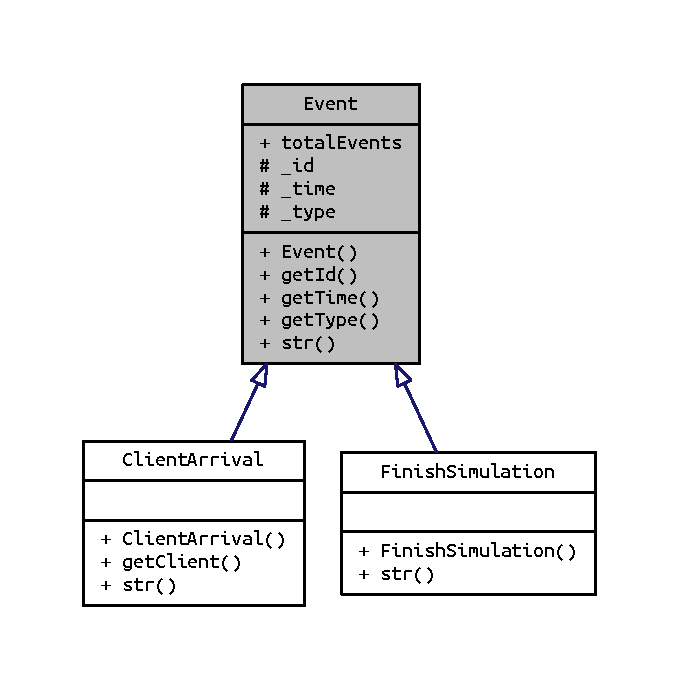
\includegraphics[width=252pt]{class_event__inherit__graph}
\end{center}
\end{figure}


Collaboration diagram for Event\+:
\nopagebreak
\begin{figure}[H]
\begin{center}
\leavevmode
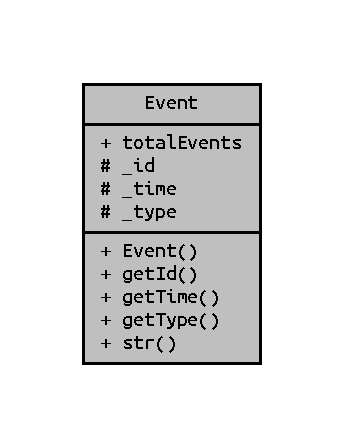
\includegraphics[width=119pt]{class_event__coll__graph}
\end{center}
\end{figure}
\subsection*{Public Member Functions}
\begin{DoxyCompactItemize}
\item 
{\bf Event} (unsigned long time, {\bf Event\+Type} type)
\item 
unsigned long {\bf get\+Id} () const 
\item 
unsigned long {\bf get\+Time} () const 
\item 
{\bf Event\+Type} {\bf get\+Type} () const 
\item 
virtual std\+::string {\bf str} () const 
\end{DoxyCompactItemize}
\subsection*{Static Public Attributes}
\begin{DoxyCompactItemize}
\item 
static unsigned long {\bf total\+Events} = 0
\end{DoxyCompactItemize}
\subsection*{Protected Attributes}
\begin{DoxyCompactItemize}
\item 
unsigned long {\bf \+\_\+id}
\item 
unsigned long {\bf \+\_\+time}
\item 
{\bf Event\+Type} {\bf \+\_\+type}
\end{DoxyCompactItemize}


\subsection{Detailed Description}


Definition at line 6 of file Event.\+h.



\subsection{Constructor \& Destructor Documentation}
\index{Event@{Event}!Event@{Event}}
\index{Event@{Event}!Event@{Event}}
\subsubsection[{Event}]{\setlength{\rightskip}{0pt plus 5cm}Event\+::\+Event (
\begin{DoxyParamCaption}
\item[{unsigned long}]{time, }
\item[{{\bf Event\+Type}}]{type}
\end{DoxyParamCaption}
)}\label{class_event_a81ced98f0e668acac3d43d2198981b33}


Definition at line 6 of file Event.\+cpp.



\subsection{Member Function Documentation}
\index{Event@{Event}!get\+Id@{get\+Id}}
\index{get\+Id@{get\+Id}!Event@{Event}}
\subsubsection[{get\+Id}]{\setlength{\rightskip}{0pt plus 5cm}unsigned long Event\+::get\+Id (
\begin{DoxyParamCaption}
{}
\end{DoxyParamCaption}
) const}\label{class_event_a973b98b35d66d83449ee370f17b8f987}


Definition at line 9 of file Event.\+cpp.



Here is the caller graph for this function\+:
\nopagebreak
\begin{figure}[H]
\begin{center}
\leavevmode
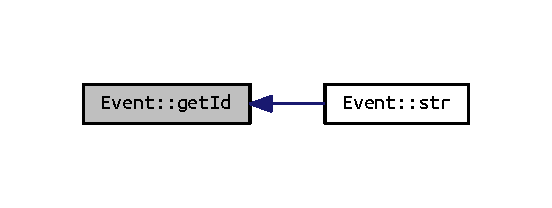
\includegraphics[width=209pt]{class_event_a973b98b35d66d83449ee370f17b8f987_icgraph}
\end{center}
\end{figure}


\index{Event@{Event}!get\+Time@{get\+Time}}
\index{get\+Time@{get\+Time}!Event@{Event}}
\subsubsection[{get\+Time}]{\setlength{\rightskip}{0pt plus 5cm}unsigned long Event\+::get\+Time (
\begin{DoxyParamCaption}
{}
\end{DoxyParamCaption}
) const}\label{class_event_a3068db436fce856e0499edcd1eb88a3d}


Definition at line 11 of file Event.\+cpp.

\index{Event@{Event}!get\+Type@{get\+Type}}
\index{get\+Type@{get\+Type}!Event@{Event}}
\subsubsection[{get\+Type}]{\setlength{\rightskip}{0pt plus 5cm}{\bf Event\+Type} Event\+::get\+Type (
\begin{DoxyParamCaption}
{}
\end{DoxyParamCaption}
) const}\label{class_event_ab0c2e30730d5859851f3126258c0126e}


Definition at line 13 of file Event.\+cpp.



Here is the caller graph for this function\+:
\nopagebreak
\begin{figure}[H]
\begin{center}
\leavevmode
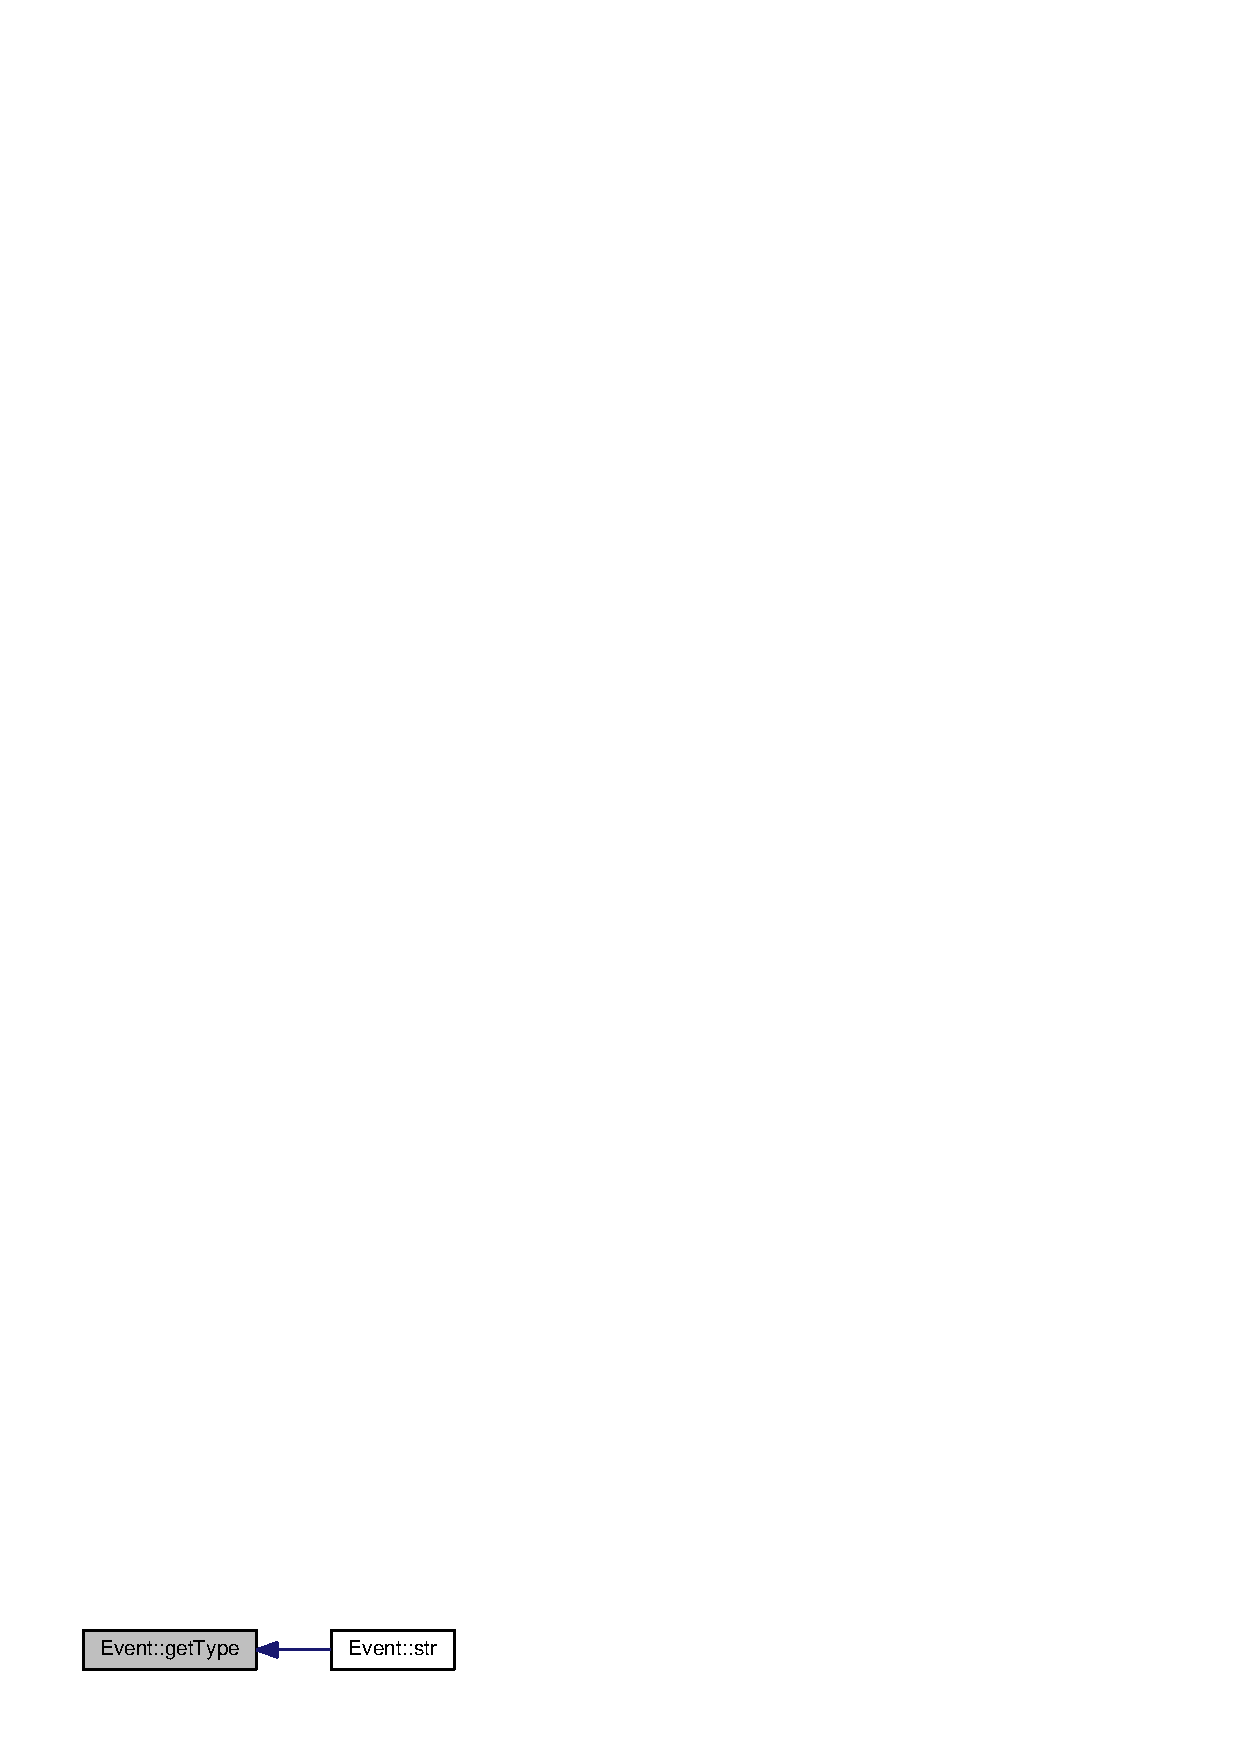
\includegraphics[width=222pt]{class_event_ab0c2e30730d5859851f3126258c0126e_icgraph}
\end{center}
\end{figure}


\index{Event@{Event}!str@{str}}
\index{str@{str}!Event@{Event}}
\subsubsection[{str}]{\setlength{\rightskip}{0pt plus 5cm}std\+::string Event\+::str (
\begin{DoxyParamCaption}
{}
\end{DoxyParamCaption}
) const\hspace{0.3cm}{\ttfamily [virtual]}}\label{class_event_abf16ed4a9c78514c704ce2de6a2b9ec7}


Reimplemented in {\bf Client\+Arrival} \doxyref{}{p.}{class_client_arrival_aed100adfc8eaf083194ac0c630eaafe6}, and {\bf Finish\+Simulation} \doxyref{}{p.}{class_finish_simulation_a8d708e0f4827daedf79a6098dd00eda4}.



Definition at line 15 of file Event.\+cpp.



Here is the call graph for this function\+:
\nopagebreak
\begin{figure}[H]
\begin{center}
\leavevmode
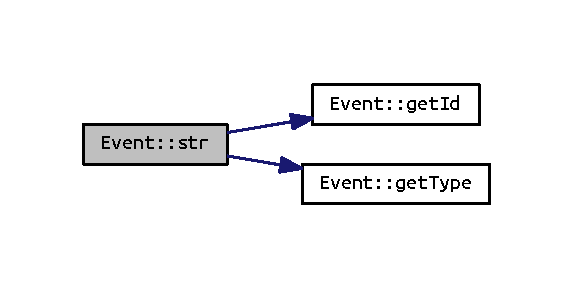
\includegraphics[width=267pt]{class_event_abf16ed4a9c78514c704ce2de6a2b9ec7_cgraph}
\end{center}
\end{figure}




\subsection{Member Data Documentation}
\index{Event@{Event}!\+\_\+id@{\+\_\+id}}
\index{\+\_\+id@{\+\_\+id}!Event@{Event}}
\subsubsection[{\+\_\+id}]{\setlength{\rightskip}{0pt plus 5cm}unsigned long Event\+::\+\_\+id\hspace{0.3cm}{\ttfamily [protected]}}\label{class_event_a3a2f9bab41280ee0d767ec8390b1812a}


Definition at line 18 of file Event.\+h.

\index{Event@{Event}!\+\_\+time@{\+\_\+time}}
\index{\+\_\+time@{\+\_\+time}!Event@{Event}}
\subsubsection[{\+\_\+time}]{\setlength{\rightskip}{0pt plus 5cm}unsigned long Event\+::\+\_\+time\hspace{0.3cm}{\ttfamily [protected]}}\label{class_event_a07e28c531b6374af308c059990938bf5}


Definition at line 19 of file Event.\+h.

\index{Event@{Event}!\+\_\+type@{\+\_\+type}}
\index{\+\_\+type@{\+\_\+type}!Event@{Event}}
\subsubsection[{\+\_\+type}]{\setlength{\rightskip}{0pt plus 5cm}{\bf Event\+Type} Event\+::\+\_\+type\hspace{0.3cm}{\ttfamily [protected]}}\label{class_event_ac39a6517d8bfadbb3bbaf97a077a5cdf}


Definition at line 20 of file Event.\+h.

\index{Event@{Event}!total\+Events@{total\+Events}}
\index{total\+Events@{total\+Events}!Event@{Event}}
\subsubsection[{total\+Events}]{\setlength{\rightskip}{0pt plus 5cm}unsigned long Event\+::total\+Events = 0\hspace{0.3cm}{\ttfamily [static]}}\label{class_event_af56653a3bf07521930251f7f93391cef}


Definition at line 8 of file Event.\+h.



The documentation for this class was generated from the following files\+:\begin{DoxyCompactItemize}
\item 
include/{\bf Event.\+h}\item 
src/{\bf Event.\+cpp}\end{DoxyCompactItemize}

\hypertarget{class_event_comparator}{}\section{Event\+Comparator Class Reference}
\label{class_event_comparator}\index{Event\+Comparator@{Event\+Comparator}}


{\ttfamily \#include $<$Event\+Comparator.\+h$>$}



Collaboration diagram for Event\+Comparator\+:
\nopagebreak
\begin{figure}[H]
\begin{center}
\leavevmode
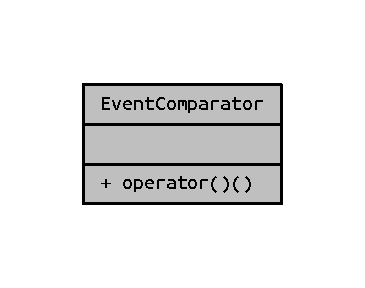
\includegraphics[width=175pt]{class_event_comparator__coll__graph}
\end{center}
\end{figure}
\subsection*{Public Member Functions}
\begin{DoxyCompactItemize}
\item 
bool \hyperlink{class_event_comparator_acb6d90290ac7d2de284009887f2dabdc}{operator()} (std\+::shared\+\_\+ptr$<$ const \hyperlink{class_event}{Event} $>$ e1, std\+::shared\+\_\+ptr$<$ const \hyperlink{class_event}{Event} $>$ e2) const 
\end{DoxyCompactItemize}


\subsection{Member Function Documentation}
\hypertarget{class_event_comparator_acb6d90290ac7d2de284009887f2dabdc}{}\index{Event\+Comparator@{Event\+Comparator}!operator()@{operator()}}
\index{operator()@{operator()}!Event\+Comparator@{Event\+Comparator}}
\subsubsection[{operator()}]{\setlength{\rightskip}{0pt plus 5cm}bool Event\+Comparator\+::operator() (
\begin{DoxyParamCaption}
\item[{std\+::shared\+\_\+ptr$<$ const {\bf Event} $>$}]{e1, }
\item[{std\+::shared\+\_\+ptr$<$ const {\bf Event} $>$}]{e2}
\end{DoxyParamCaption}
) const}\label{class_event_comparator_acb6d90290ac7d2de284009887f2dabdc}


The documentation for this class was generated from the following files\+:\begin{DoxyCompactItemize}
\item 
include/\hyperlink{_event_comparator_8h}{Event\+Comparator.\+h}\item 
src/\hyperlink{_event_comparator_8cpp}{Event\+Comparator.\+cpp}\end{DoxyCompactItemize}

\section{Event\+Dispatcher Class Reference}
\label{class_event_dispatcher}\index{Event\+Dispatcher@{Event\+Dispatcher}}


{\ttfamily \#include $<$Event\+Dispatcher.\+h$>$}



Inheritance diagram for Event\+Dispatcher\+:
\nopagebreak
\begin{figure}[H]
\begin{center}
\leavevmode
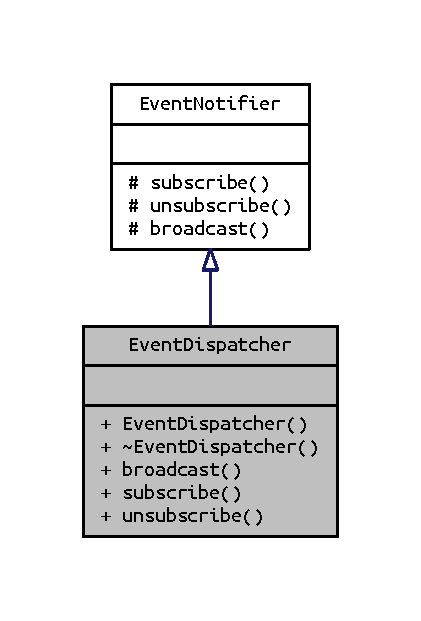
\includegraphics[width=154pt]{class_event_dispatcher__inherit__graph}
\end{center}
\end{figure}


Collaboration diagram for Event\+Dispatcher\+:
\nopagebreak
\begin{figure}[H]
\begin{center}
\leavevmode
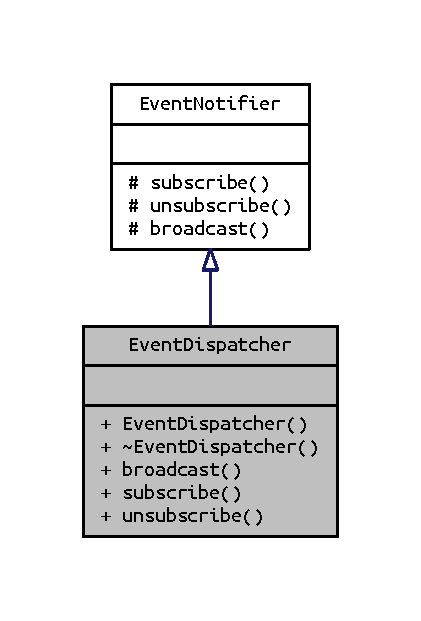
\includegraphics[width=154pt]{class_event_dispatcher__coll__graph}
\end{center}
\end{figure}
\subsection*{Public Member Functions}
\begin{DoxyCompactItemize}
\item 
{\bf Event\+Dispatcher} ()
\item 
virtual {\bf $\sim$\+Event\+Dispatcher} ()
\item 
void {\bf broadcast} (const std\+::shared\+\_\+ptr$<$ const {\bf Event} $>$ event) const 
\item 
void {\bf subscribe} (std\+::shared\+\_\+ptr$<$ {\bf Event\+Observer} $>$ event\+Observer)
\item 
void {\bf unsubscribe} (std\+::shared\+\_\+ptr$<$ {\bf Event\+Observer} $>$ event\+Observer)
\end{DoxyCompactItemize}
\subsection*{Additional Inherited Members}


\subsection{Detailed Description}


Definition at line 10 of file Event\+Dispatcher.\+h.



\subsection{Constructor \& Destructor Documentation}
\index{Event\+Dispatcher@{Event\+Dispatcher}!Event\+Dispatcher@{Event\+Dispatcher}}
\index{Event\+Dispatcher@{Event\+Dispatcher}!Event\+Dispatcher@{Event\+Dispatcher}}
\subsubsection[{Event\+Dispatcher}]{\setlength{\rightskip}{0pt plus 5cm}Event\+Dispatcher\+::\+Event\+Dispatcher (
\begin{DoxyParamCaption}
{}
\end{DoxyParamCaption}
)}\label{class_event_dispatcher_aec174a9e25796e5727e59f5452817cda}


Definition at line 6 of file Event\+Dispatcher.\+cpp.

\index{Event\+Dispatcher@{Event\+Dispatcher}!````~Event\+Dispatcher@{$\sim$\+Event\+Dispatcher}}
\index{````~Event\+Dispatcher@{$\sim$\+Event\+Dispatcher}!Event\+Dispatcher@{Event\+Dispatcher}}
\subsubsection[{$\sim$\+Event\+Dispatcher}]{\setlength{\rightskip}{0pt plus 5cm}Event\+Dispatcher\+::$\sim$\+Event\+Dispatcher (
\begin{DoxyParamCaption}
{}
\end{DoxyParamCaption}
)\hspace{0.3cm}{\ttfamily [virtual]}}\label{class_event_dispatcher_abb5f401014e87f03027d6c4450964e55}


Definition at line 8 of file Event\+Dispatcher.\+cpp.



\subsection{Member Function Documentation}
\index{Event\+Dispatcher@{Event\+Dispatcher}!broadcast@{broadcast}}
\index{broadcast@{broadcast}!Event\+Dispatcher@{Event\+Dispatcher}}
\subsubsection[{broadcast}]{\setlength{\rightskip}{0pt plus 5cm}void Event\+Dispatcher\+::broadcast (
\begin{DoxyParamCaption}
\item[{const std\+::shared\+\_\+ptr$<$ const {\bf Event} $>$}]{event}
\end{DoxyParamCaption}
) const\hspace{0.3cm}{\ttfamily [virtual]}}\label{class_event_dispatcher_a2664ed4e9f1eca1f239bbd40add82f45}


Implements {\bf Event\+Notifier} \doxyref{}{p.}{class_event_notifier_af6a63fe66700be838c3027bba458294a}.



Definition at line 10 of file Event\+Dispatcher.\+cpp.

\index{Event\+Dispatcher@{Event\+Dispatcher}!subscribe@{subscribe}}
\index{subscribe@{subscribe}!Event\+Dispatcher@{Event\+Dispatcher}}
\subsubsection[{subscribe}]{\setlength{\rightskip}{0pt plus 5cm}void Event\+Dispatcher\+::subscribe (
\begin{DoxyParamCaption}
\item[{std\+::shared\+\_\+ptr$<$ {\bf Event\+Observer} $>$}]{event\+Observer}
\end{DoxyParamCaption}
)\hspace{0.3cm}{\ttfamily [virtual]}}\label{class_event_dispatcher_a0cd1157fb6213be48fbdadc749088231}


Implements {\bf Event\+Notifier} \doxyref{}{p.}{class_event_notifier_a769469c36337d28f08cc5b7250885a0c}.



Definition at line 18 of file Event\+Dispatcher.\+cpp.

\index{Event\+Dispatcher@{Event\+Dispatcher}!unsubscribe@{unsubscribe}}
\index{unsubscribe@{unsubscribe}!Event\+Dispatcher@{Event\+Dispatcher}}
\subsubsection[{unsubscribe}]{\setlength{\rightskip}{0pt plus 5cm}void Event\+Dispatcher\+::unsubscribe (
\begin{DoxyParamCaption}
\item[{std\+::shared\+\_\+ptr$<$ {\bf Event\+Observer} $>$}]{event\+Observer}
\end{DoxyParamCaption}
)\hspace{0.3cm}{\ttfamily [virtual]}}\label{class_event_dispatcher_a3242f22a220dd58964835544c799c4fa}


Implements {\bf Event\+Notifier} \doxyref{}{p.}{class_event_notifier_a80e222d382981380c86cd61c52142e78}.



Definition at line 23 of file Event\+Dispatcher.\+cpp.



The documentation for this class was generated from the following files\+:\begin{DoxyCompactItemize}
\item 
include/{\bf Event\+Dispatcher.\+h}\item 
src/{\bf Event\+Dispatcher.\+cpp}\end{DoxyCompactItemize}

\section{Event\+Factory Class Reference}
\label{class_event_factory}\index{Event\+Factory@{Event\+Factory}}


{\ttfamily \#include $<$Event\+Factory.\+h$>$}



Collaboration diagram for Event\+Factory\+:
\nopagebreak
\begin{figure}[H]
\begin{center}
\leavevmode
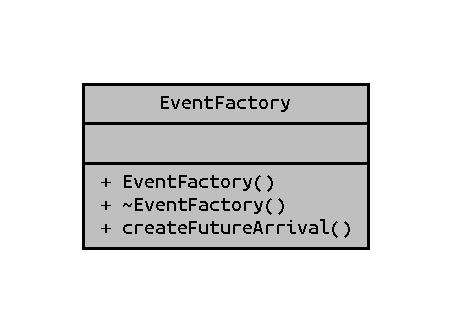
\includegraphics[width=158pt]{class_event_factory__coll__graph}
\end{center}
\end{figure}
\subsection*{Public Member Functions}
\begin{DoxyCompactItemize}
\item 
{\bf Event\+Factory} (std\+::shared\+\_\+ptr$<$ {\bf Clock} $>$ clock, std\+::shared\+\_\+ptr$<$ {\bf Floor} $>$ floor, std\+::shared\+\_\+ptr$<$ const {\bf Scenario} $>$ scenario, std\+::shared\+\_\+ptr$<$ std\+::mt19937 $>$ random\+\_\+engine)
\item 
virtual {\bf $\sim$\+Event\+Factory} ()
\item 
void {\bf create\+Future\+Arrival} (const std\+::shared\+\_\+ptr$<$ {\bf Event\+Queue} $>$ event\+Queue)
\end{DoxyCompactItemize}


\subsection{Detailed Description}


Definition at line 13 of file Event\+Factory.\+h.



\subsection{Constructor \& Destructor Documentation}
\index{Event\+Factory@{Event\+Factory}!Event\+Factory@{Event\+Factory}}
\index{Event\+Factory@{Event\+Factory}!Event\+Factory@{Event\+Factory}}
\subsubsection[{Event\+Factory}]{\setlength{\rightskip}{0pt plus 5cm}Event\+Factory\+::\+Event\+Factory (
\begin{DoxyParamCaption}
\item[{std\+::shared\+\_\+ptr$<$ {\bf Clock} $>$}]{clock, }
\item[{std\+::shared\+\_\+ptr$<$ {\bf Floor} $>$}]{floor, }
\item[{std\+::shared\+\_\+ptr$<$ const {\bf Scenario} $>$}]{scenario, }
\item[{std\+::shared\+\_\+ptr$<$ std\+::mt19937 $>$}]{random\+\_\+engine}
\end{DoxyParamCaption}
)}\label{class_event_factory_ace922ce2886db334e0910b59ffd03c69}


Definition at line 9 of file Event\+Factory.\+cpp.

\index{Event\+Factory@{Event\+Factory}!````~Event\+Factory@{$\sim$\+Event\+Factory}}
\index{````~Event\+Factory@{$\sim$\+Event\+Factory}!Event\+Factory@{Event\+Factory}}
\subsubsection[{$\sim$\+Event\+Factory}]{\setlength{\rightskip}{0pt plus 5cm}Event\+Factory\+::$\sim$\+Event\+Factory (
\begin{DoxyParamCaption}
{}
\end{DoxyParamCaption}
)\hspace{0.3cm}{\ttfamily [virtual]}}\label{class_event_factory_ab4e7ee369071e7adb5aeb629d8b615e4}


Definition at line 21 of file Event\+Factory.\+cpp.



\subsection{Member Function Documentation}
\index{Event\+Factory@{Event\+Factory}!create\+Future\+Arrival@{create\+Future\+Arrival}}
\index{create\+Future\+Arrival@{create\+Future\+Arrival}!Event\+Factory@{Event\+Factory}}
\subsubsection[{create\+Future\+Arrival}]{\setlength{\rightskip}{0pt plus 5cm}void Event\+Factory\+::create\+Future\+Arrival (
\begin{DoxyParamCaption}
\item[{const std\+::shared\+\_\+ptr$<$ {\bf Event\+Queue} $>$}]{event\+Queue}
\end{DoxyParamCaption}
)}\label{class_event_factory_aa1e884d273b411a9e8265b774e6bfa8e}


Definition at line 23 of file Event\+Factory.\+cpp.



The documentation for this class was generated from the following files\+:\begin{DoxyCompactItemize}
\item 
include/{\bf Event\+Factory.\+h}\item 
src/{\bf Event\+Factory.\+cpp}\end{DoxyCompactItemize}

\section{Event\+Notifier Class Reference}
\label{class_event_notifier}\index{Event\+Notifier@{Event\+Notifier}}


{\ttfamily \#include $<$Event\+Notifier.\+h$>$}



Inheritance diagram for Event\+Notifier\+:\nopagebreak
\begin{figure}[H]
\begin{center}
\leavevmode
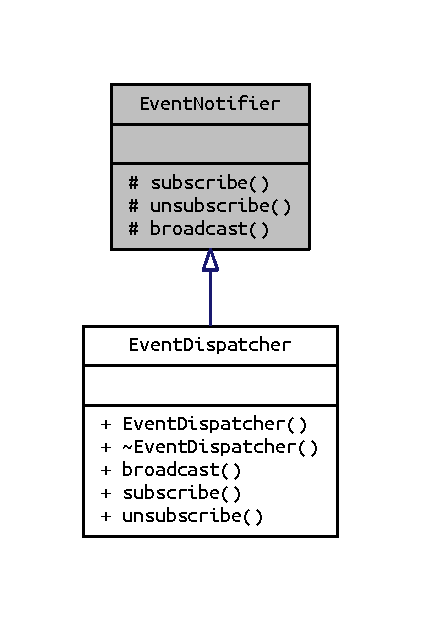
\includegraphics[width=154pt]{class_event_notifier__inherit__graph}
\end{center}
\end{figure}


Collaboration diagram for Event\+Notifier\+:\nopagebreak
\begin{figure}[H]
\begin{center}
\leavevmode
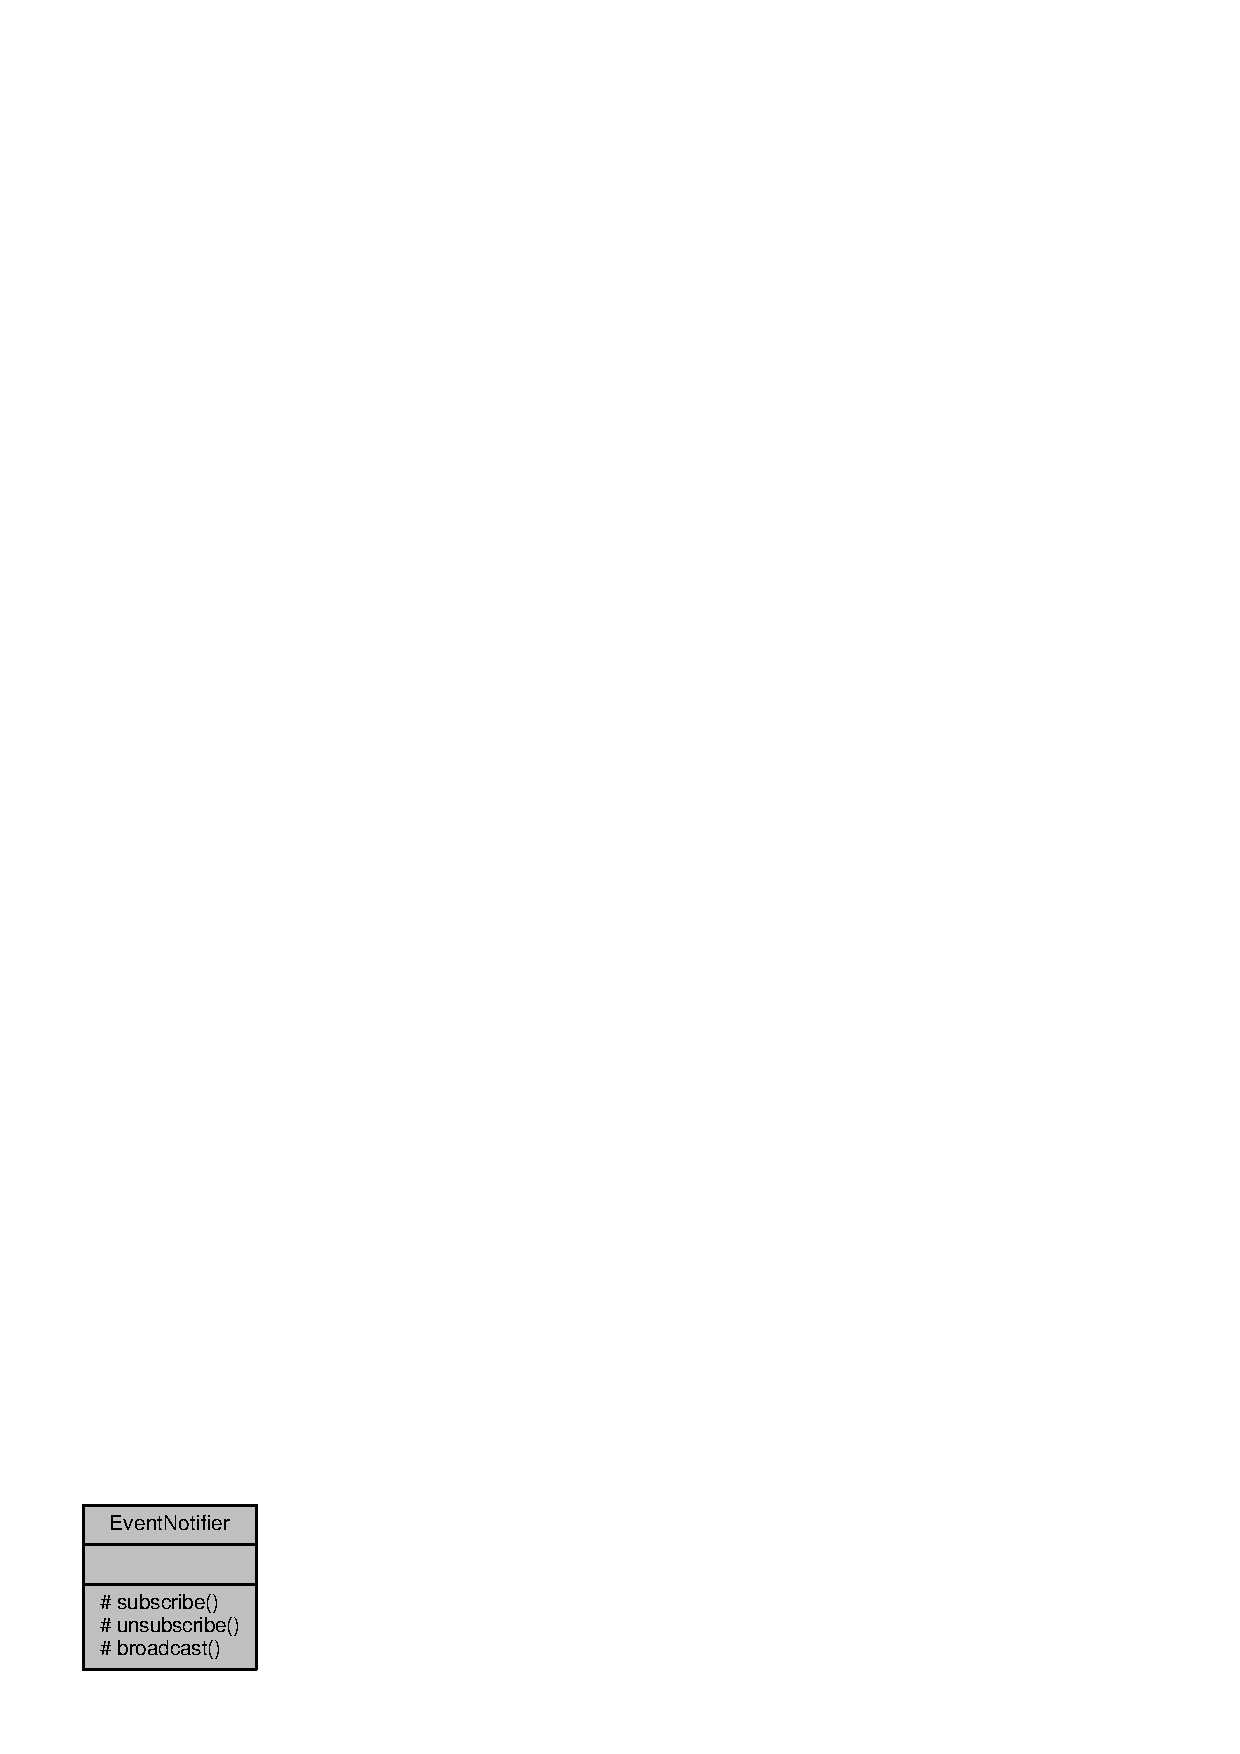
\includegraphics[width=127pt]{class_event_notifier__coll__graph}
\end{center}
\end{figure}
\subsection*{Protected Member Functions}
\begin{DoxyCompactItemize}
\item 
virtual void {\bf subscribe} (std\+::shared\+\_\+ptr$<$ {\bf Event\+Observer} $>$ observer)=0
\item 
virtual void {\bf unsubscribe} (std\+::shared\+\_\+ptr$<$ {\bf Event\+Observer} $>$ observer)=0
\item 
virtual void {\bf broadcast} (const std\+::shared\+\_\+ptr$<$ const {\bf Event} $>$ event) const =0
\end{DoxyCompactItemize}


\subsection{Detailed Description}


Definition at line 8 of file Event\+Notifier.\+h.



\subsection{Member Function Documentation}
\index{Event\+Notifier@{Event\+Notifier}!broadcast@{broadcast}}
\index{broadcast@{broadcast}!Event\+Notifier@{Event\+Notifier}}
\subsubsection[{broadcast}]{\setlength{\rightskip}{0pt plus 5cm}virtual void Event\+Notifier\+::broadcast (
\begin{DoxyParamCaption}
\item[{const std\+::shared\+\_\+ptr$<$ const {\bf Event} $>$}]{event}
\end{DoxyParamCaption}
) const\hspace{0.3cm}{\ttfamily [protected]}, {\ttfamily [pure virtual]}}\label{class_event_notifier_af6a63fe66700be838c3027bba458294a}


Implemented in {\bf Event\+Dispatcher} \doxyref{}{p.}{class_event_dispatcher_a2664ed4e9f1eca1f239bbd40add82f45}.

\index{Event\+Notifier@{Event\+Notifier}!subscribe@{subscribe}}
\index{subscribe@{subscribe}!Event\+Notifier@{Event\+Notifier}}
\subsubsection[{subscribe}]{\setlength{\rightskip}{0pt plus 5cm}virtual void Event\+Notifier\+::subscribe (
\begin{DoxyParamCaption}
\item[{std\+::shared\+\_\+ptr$<$ {\bf Event\+Observer} $>$}]{observer}
\end{DoxyParamCaption}
)\hspace{0.3cm}{\ttfamily [protected]}, {\ttfamily [pure virtual]}}\label{class_event_notifier_a769469c36337d28f08cc5b7250885a0c}


Implemented in {\bf Event\+Dispatcher} \doxyref{}{p.}{class_event_dispatcher_a0cd1157fb6213be48fbdadc749088231}.

\index{Event\+Notifier@{Event\+Notifier}!unsubscribe@{unsubscribe}}
\index{unsubscribe@{unsubscribe}!Event\+Notifier@{Event\+Notifier}}
\subsubsection[{unsubscribe}]{\setlength{\rightskip}{0pt plus 5cm}virtual void Event\+Notifier\+::unsubscribe (
\begin{DoxyParamCaption}
\item[{std\+::shared\+\_\+ptr$<$ {\bf Event\+Observer} $>$}]{observer}
\end{DoxyParamCaption}
)\hspace{0.3cm}{\ttfamily [protected]}, {\ttfamily [pure virtual]}}\label{class_event_notifier_a80e222d382981380c86cd61c52142e78}


Implemented in {\bf Event\+Dispatcher} \doxyref{}{p.}{class_event_dispatcher_a3242f22a220dd58964835544c799c4fa}.



The documentation for this class was generated from the following file\+:\begin{DoxyCompactItemize}
\item 
include/{\bf Event\+Notifier.\+h}\end{DoxyCompactItemize}

\section{Event\+Observer Class Reference}
\label{class_event_observer}\index{Event\+Observer@{Event\+Observer}}


{\ttfamily \#include $<$Event\+Observer.\+h$>$}



Inheritance diagram for Event\+Observer\+:\nopagebreak
\begin{figure}[H]
\begin{center}
\leavevmode
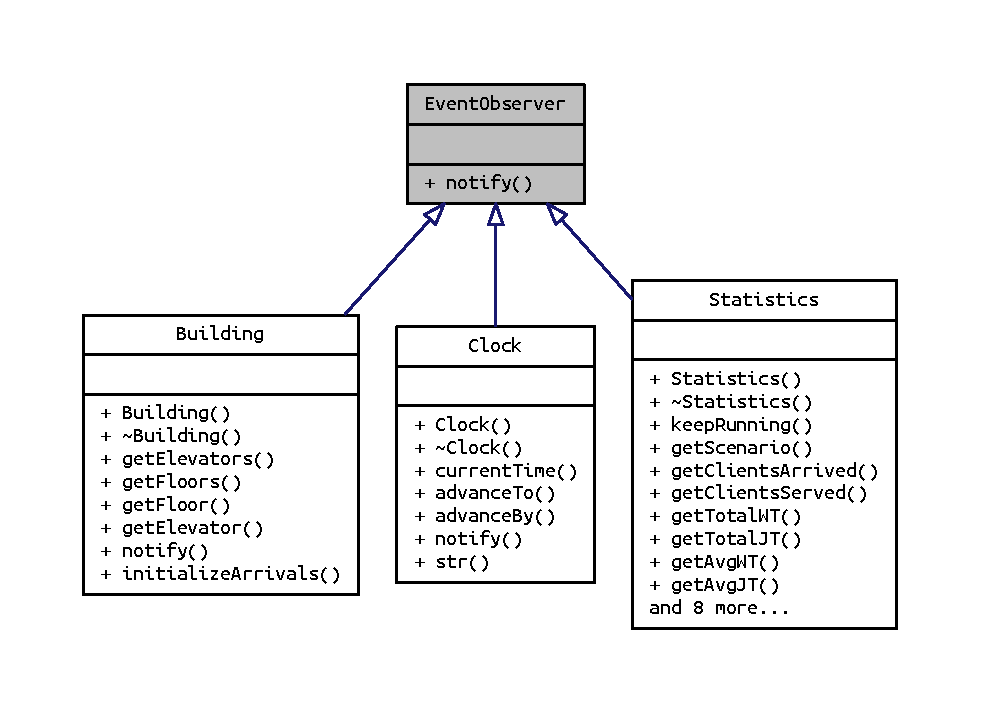
\includegraphics[width=350pt]{class_event_observer__inherit__graph}
\end{center}
\end{figure}


Collaboration diagram for Event\+Observer\+:\nopagebreak
\begin{figure}[H]
\begin{center}
\leavevmode
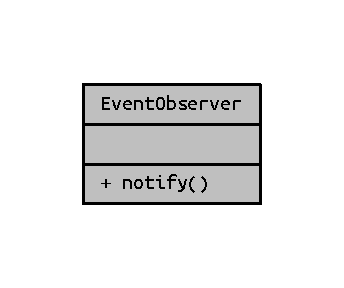
\includegraphics[width=126pt]{class_event_observer__coll__graph}
\end{center}
\end{figure}
\subsection*{Public Member Functions}
\begin{DoxyCompactItemize}
\item 
virtual void {\bf notify} (const std\+::shared\+\_\+ptr$<$ const {\bf Event} $>$ event)=0
\end{DoxyCompactItemize}


\subsection{Detailed Description}


Definition at line 7 of file Event\+Observer.\+h.



\subsection{Member Function Documentation}
\index{Event\+Observer@{Event\+Observer}!notify@{notify}}
\index{notify@{notify}!Event\+Observer@{Event\+Observer}}
\subsubsection[{notify}]{\setlength{\rightskip}{0pt plus 5cm}virtual void Event\+Observer\+::notify (
\begin{DoxyParamCaption}
\item[{const std\+::shared\+\_\+ptr$<$ const {\bf Event} $>$}]{event}
\end{DoxyParamCaption}
)\hspace{0.3cm}{\ttfamily [pure virtual]}}\label{class_event_observer_a81b3c545084ba3c8eaa8c83f5a0a4eb8}


Implemented in {\bf Building} \doxyref{}{p.}{class_building_a380e65fcb24d40d82077edc0572df3c1}, {\bf Statistics} \doxyref{}{p.}{class_statistics_a75d0a1191341fe95e94bf50a6b69a5a3}, and {\bf Clock} \doxyref{}{p.}{class_clock_a534758881637b06f765a24af22f9e8a1}.



The documentation for this class was generated from the following file\+:\begin{DoxyCompactItemize}
\item 
include/{\bf Event\+Observer.\+h}\end{DoxyCompactItemize}

\hypertarget{class_event_queue}{}\section{Event\+Queue Class Reference}
\label{class_event_queue}\index{Event\+Queue@{Event\+Queue}}


{\ttfamily \#include $<$Event\+Queue.\+h$>$}



Collaboration diagram for Event\+Queue\+:
\nopagebreak
\begin{figure}[H]
\begin{center}
\leavevmode
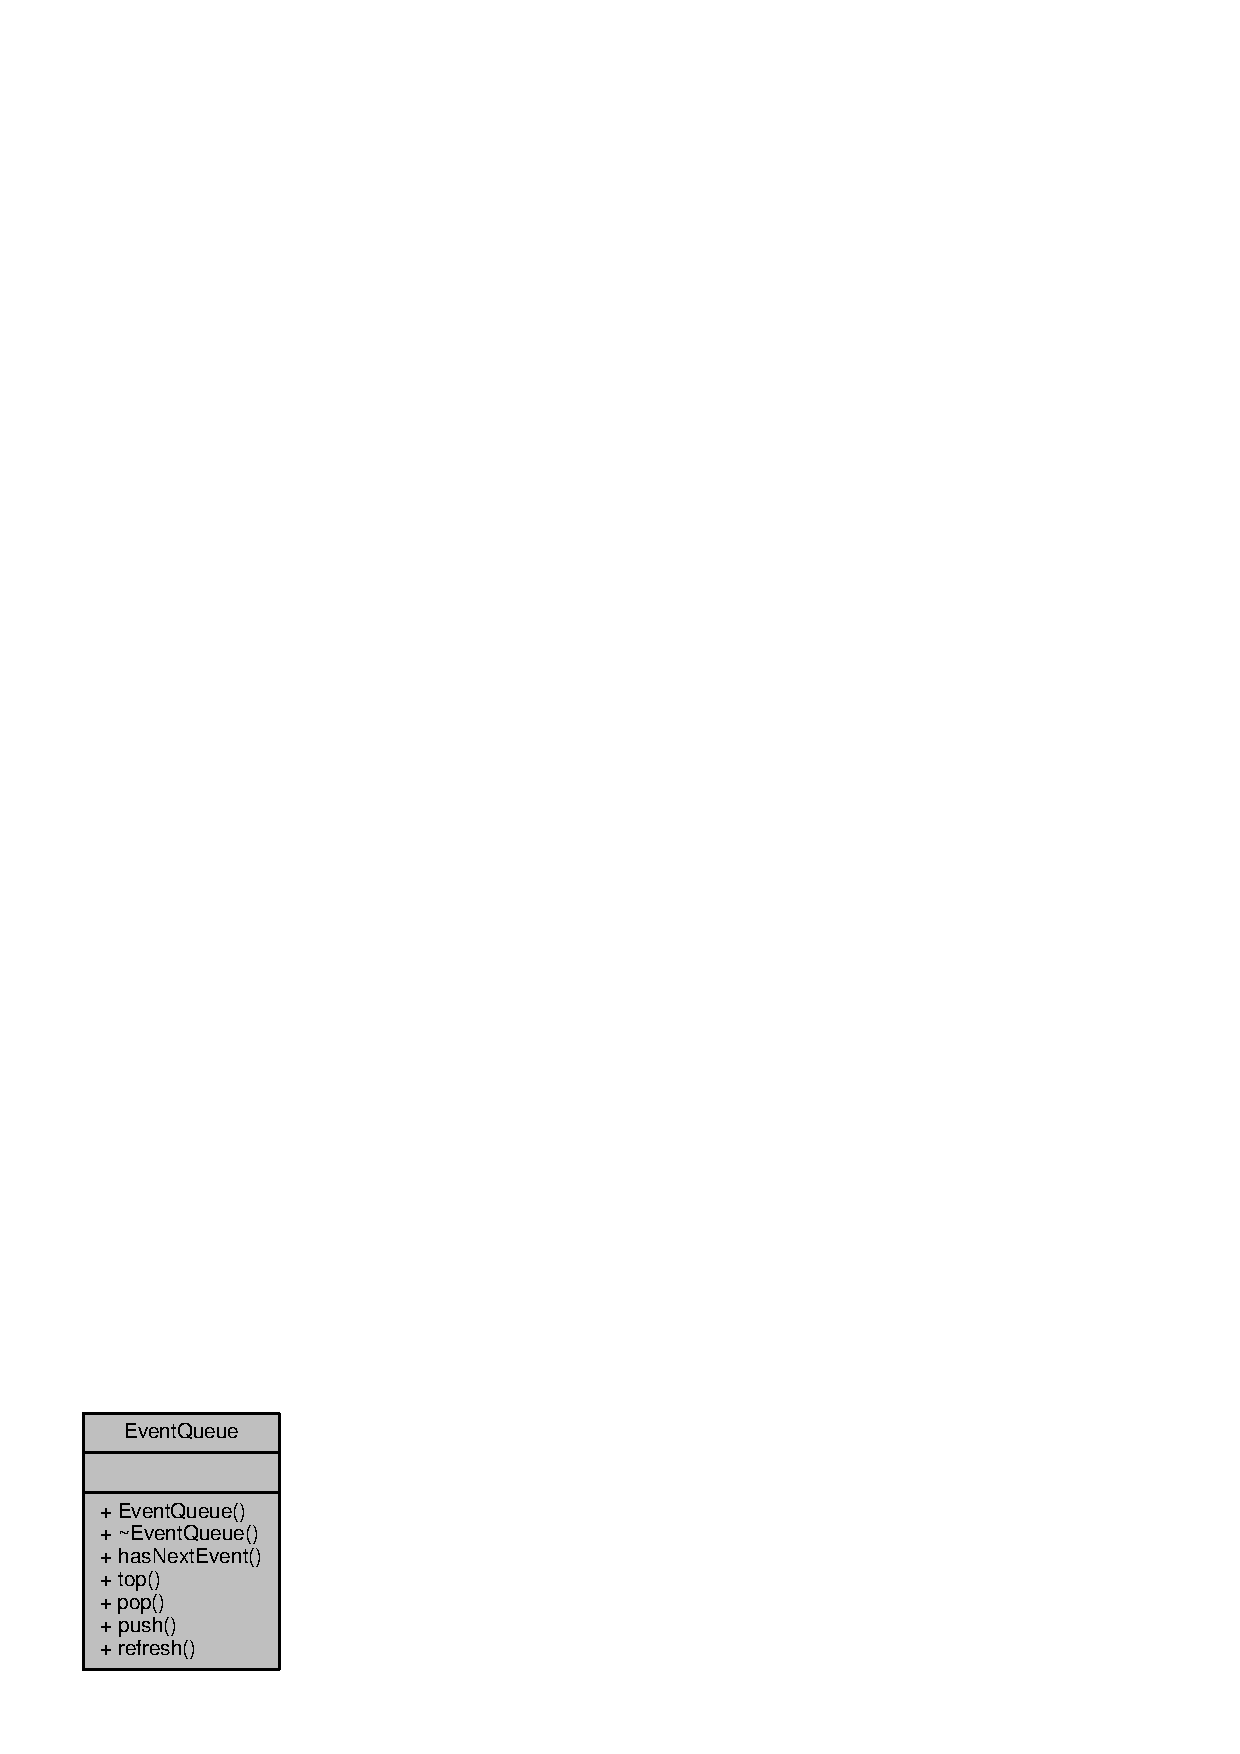
\includegraphics[width=181pt]{class_event_queue__coll__graph}
\end{center}
\end{figure}
\subsection*{Public Member Functions}
\begin{DoxyCompactItemize}
\item 
\hyperlink{class_event_queue_ab7de5a41befc94aac0f461391e67f14a}{Event\+Queue} ()
\item 
virtual \hyperlink{class_event_queue_ac57db8e2366f2c6c594e6afc975e3b59}{$\sim$\+Event\+Queue} ()
\item 
bool \hyperlink{class_event_queue_ad439103ef84d177e2cd37eab36bbb606}{has\+Next\+Event} () const 
\item 
std\+::shared\+\_\+ptr$<$ \hyperlink{class_event}{Event} $>$ \hyperlink{class_event_queue_af633f824cb4f4c3ff99d8e0601b61ce6}{top} () const 
\item 
std\+::shared\+\_\+ptr$<$ \hyperlink{class_event}{Event} $>$ \hyperlink{class_event_queue_a63042846b35c5071f876ceecbfe56ade}{pop} ()
\item 
void \hyperlink{class_event_queue_a826f8fd05053a782f45c568feb76dbd7}{push} (std\+::shared\+\_\+ptr$<$ \hyperlink{class_event}{Event} $>$ event)
\item 
void \hyperlink{class_event_queue_a0a9d0f11be898266a61bbd8d569369a5}{refresh} (const unsigned long current\+Time)
\end{DoxyCompactItemize}


\subsection{Constructor \& Destructor Documentation}
\hypertarget{class_event_queue_ab7de5a41befc94aac0f461391e67f14a}{}\index{Event\+Queue@{Event\+Queue}!Event\+Queue@{Event\+Queue}}
\index{Event\+Queue@{Event\+Queue}!Event\+Queue@{Event\+Queue}}
\subsubsection[{Event\+Queue}]{\setlength{\rightskip}{0pt plus 5cm}Event\+Queue\+::\+Event\+Queue (
\begin{DoxyParamCaption}
{}
\end{DoxyParamCaption}
)}\label{class_event_queue_ab7de5a41befc94aac0f461391e67f14a}
\hypertarget{class_event_queue_ac57db8e2366f2c6c594e6afc975e3b59}{}\index{Event\+Queue@{Event\+Queue}!````~Event\+Queue@{$\sim$\+Event\+Queue}}
\index{````~Event\+Queue@{$\sim$\+Event\+Queue}!Event\+Queue@{Event\+Queue}}
\subsubsection[{$\sim$\+Event\+Queue}]{\setlength{\rightskip}{0pt plus 5cm}Event\+Queue\+::$\sim$\+Event\+Queue (
\begin{DoxyParamCaption}
{}
\end{DoxyParamCaption}
)\hspace{0.3cm}{\ttfamily [virtual]}}\label{class_event_queue_ac57db8e2366f2c6c594e6afc975e3b59}


\subsection{Member Function Documentation}
\hypertarget{class_event_queue_ad439103ef84d177e2cd37eab36bbb606}{}\index{Event\+Queue@{Event\+Queue}!has\+Next\+Event@{has\+Next\+Event}}
\index{has\+Next\+Event@{has\+Next\+Event}!Event\+Queue@{Event\+Queue}}
\subsubsection[{has\+Next\+Event}]{\setlength{\rightskip}{0pt plus 5cm}bool Event\+Queue\+::has\+Next\+Event (
\begin{DoxyParamCaption}
{}
\end{DoxyParamCaption}
) const}\label{class_event_queue_ad439103ef84d177e2cd37eab36bbb606}
\hypertarget{class_event_queue_a63042846b35c5071f876ceecbfe56ade}{}\index{Event\+Queue@{Event\+Queue}!pop@{pop}}
\index{pop@{pop}!Event\+Queue@{Event\+Queue}}
\subsubsection[{pop}]{\setlength{\rightskip}{0pt plus 5cm}std\+::shared\+\_\+ptr$<$ {\bf Event} $>$ Event\+Queue\+::pop (
\begin{DoxyParamCaption}
{}
\end{DoxyParamCaption}
)}\label{class_event_queue_a63042846b35c5071f876ceecbfe56ade}
\hypertarget{class_event_queue_a826f8fd05053a782f45c568feb76dbd7}{}\index{Event\+Queue@{Event\+Queue}!push@{push}}
\index{push@{push}!Event\+Queue@{Event\+Queue}}
\subsubsection[{push}]{\setlength{\rightskip}{0pt plus 5cm}void Event\+Queue\+::push (
\begin{DoxyParamCaption}
\item[{std\+::shared\+\_\+ptr$<$ {\bf Event} $>$}]{event}
\end{DoxyParamCaption}
)}\label{class_event_queue_a826f8fd05053a782f45c568feb76dbd7}
\hypertarget{class_event_queue_a0a9d0f11be898266a61bbd8d569369a5}{}\index{Event\+Queue@{Event\+Queue}!refresh@{refresh}}
\index{refresh@{refresh}!Event\+Queue@{Event\+Queue}}
\subsubsection[{refresh}]{\setlength{\rightskip}{0pt plus 5cm}void Event\+Queue\+::refresh (
\begin{DoxyParamCaption}
\item[{const unsigned long}]{current\+Time}
\end{DoxyParamCaption}
)}\label{class_event_queue_a0a9d0f11be898266a61bbd8d569369a5}
\hypertarget{class_event_queue_af633f824cb4f4c3ff99d8e0601b61ce6}{}\index{Event\+Queue@{Event\+Queue}!top@{top}}
\index{top@{top}!Event\+Queue@{Event\+Queue}}
\subsubsection[{top}]{\setlength{\rightskip}{0pt plus 5cm}std\+::shared\+\_\+ptr$<$ {\bf Event} $>$ Event\+Queue\+::top (
\begin{DoxyParamCaption}
{}
\end{DoxyParamCaption}
) const}\label{class_event_queue_af633f824cb4f4c3ff99d8e0601b61ce6}


The documentation for this class was generated from the following files\+:\begin{DoxyCompactItemize}
\item 
include/\hyperlink{_event_queue_8h}{Event\+Queue.\+h}\item 
src/\hyperlink{_event_queue_8cpp}{Event\+Queue.\+cpp}\end{DoxyCompactItemize}

\section{Finish\+Simulation Class Reference}
\label{class_finish_simulation}\index{Finish\+Simulation@{Finish\+Simulation}}


{\ttfamily \#include $<$Finish\+Simulation.\+h$>$}



Inheritance diagram for Finish\+Simulation\+:
\nopagebreak
\begin{figure}[H]
\begin{center}
\leavevmode
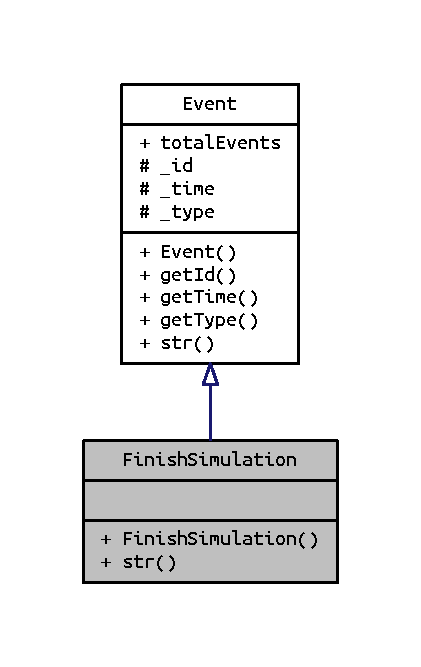
\includegraphics[width=148pt]{class_finish_simulation__inherit__graph}
\end{center}
\end{figure}


Collaboration diagram for Finish\+Simulation\+:
\nopagebreak
\begin{figure}[H]
\begin{center}
\leavevmode
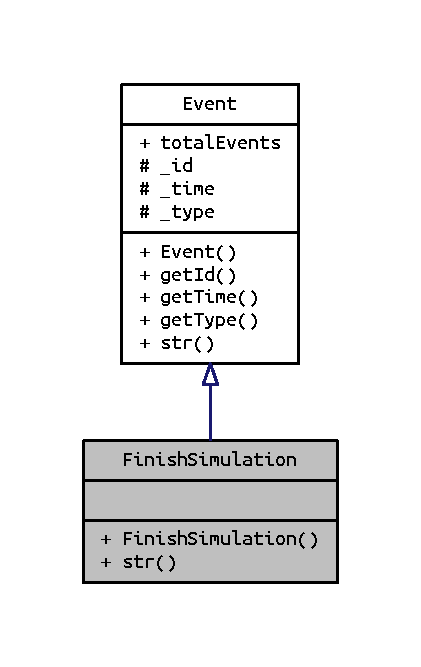
\includegraphics[width=148pt]{class_finish_simulation__coll__graph}
\end{center}
\end{figure}
\subsection*{Public Member Functions}
\begin{DoxyCompactItemize}
\item 
{\bf Finish\+Simulation} (const unsigned long event\+Time)
\item 
std\+::string {\bf str} () const 
\end{DoxyCompactItemize}
\subsection*{Additional Inherited Members}


\subsection{Detailed Description}


Definition at line 6 of file Finish\+Simulation.\+h.



\subsection{Constructor \& Destructor Documentation}
\index{Finish\+Simulation@{Finish\+Simulation}!Finish\+Simulation@{Finish\+Simulation}}
\index{Finish\+Simulation@{Finish\+Simulation}!Finish\+Simulation@{Finish\+Simulation}}
\subsubsection[{Finish\+Simulation}]{\setlength{\rightskip}{0pt plus 5cm}Finish\+Simulation\+::\+Finish\+Simulation (
\begin{DoxyParamCaption}
\item[{const unsigned long}]{event\+Time}
\end{DoxyParamCaption}
)}\label{class_finish_simulation_aafe4d56e74132af427893d49277d26b5}


Definition at line 6 of file Finish\+Simulation.\+cpp.



\subsection{Member Function Documentation}
\index{Finish\+Simulation@{Finish\+Simulation}!str@{str}}
\index{str@{str}!Finish\+Simulation@{Finish\+Simulation}}
\subsubsection[{str}]{\setlength{\rightskip}{0pt plus 5cm}std\+::string Finish\+Simulation\+::str (
\begin{DoxyParamCaption}
{}
\end{DoxyParamCaption}
) const\hspace{0.3cm}{\ttfamily [virtual]}}\label{class_finish_simulation_a8d708e0f4827daedf79a6098dd00eda4}


Reimplemented from {\bf Event} \doxyref{}{p.}{class_event_abf16ed4a9c78514c704ce2de6a2b9ec7}.



Definition at line 9 of file Finish\+Simulation.\+cpp.



The documentation for this class was generated from the following files\+:\begin{DoxyCompactItemize}
\item 
include/{\bf Finish\+Simulation.\+h}\item 
src/{\bf Finish\+Simulation.\+cpp}\end{DoxyCompactItemize}

\section{Floor Class Reference}
\label{class_floor}\index{Floor@{Floor}}


{\ttfamily \#include $<$Floor.\+h$>$}



Collaboration diagram for Floor\+:\nopagebreak
\begin{figure}[H]
\begin{center}
\leavevmode
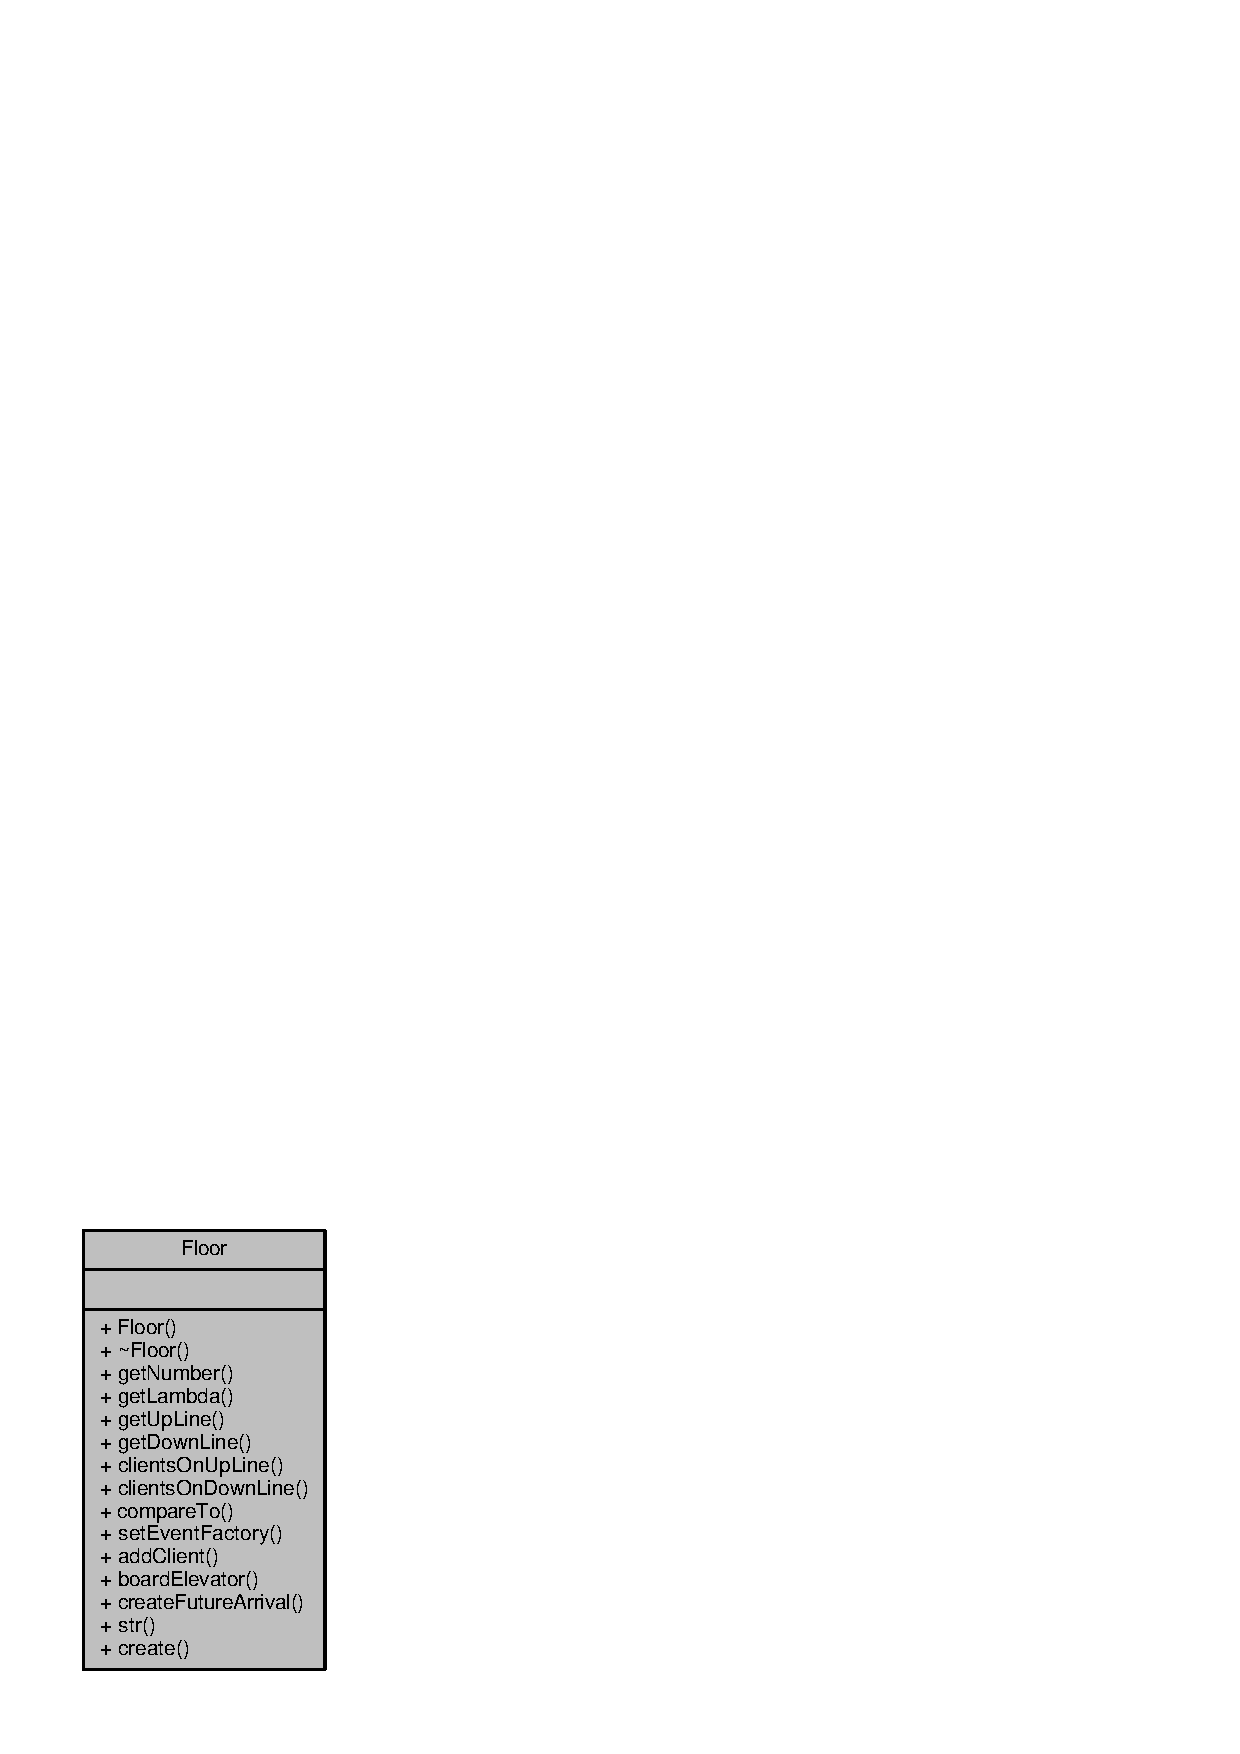
\includegraphics[width=156pt]{class_floor__coll__graph}
\end{center}
\end{figure}
\subsection*{Public Member Functions}
\begin{DoxyCompactItemize}
\item 
{\bf Floor} (const int number, const float lambda)
\item 
{\bf Floor} (const {\bf Floor} \&floor)
\item 
virtual {\bf $\sim$\+Floor} ()
\item 
int {\bf get\+Number} () const 
\item 
int {\bf get\+Lambda} () const 
\item 
std\+::queue$<$ std\+::shared\+\_\+ptr$<$ {\bf Client} $>$ $>$ {\bf get\+Up\+Line\+Copy} () const 
\item 
std\+::queue$<$ std\+::shared\+\_\+ptr$<$ {\bf Client} $>$ $>$ {\bf get\+Down\+Line\+Copy} () const 
\item 
const std\+::vector$<$ std\+::shared\+\_\+ptr$<$ {\bf Client} $>$ $>$ {\bf get\+Up\+Line} (int n) const 
\item 
const std\+::vector$<$ std\+::shared\+\_\+ptr$<$ {\bf Client} $>$ $>$ {\bf get\+Down\+Line} (int n) const 
\item 
int {\bf clients\+On\+Up\+Line} () const 
\item 
int {\bf clients\+On\+Down\+Line} () const 
\item 
{\bf Direction} {\bf compare\+To} (const {\bf Floor} \&other) const 
\item 
void {\bf set\+Event\+Factory} (const std\+::shared\+\_\+ptr$<$ {\bf Event\+Factory} $>$ event\+Factory)
\item 
{\bf Direction} {\bf add\+Client} (const std\+::shared\+\_\+ptr$<$ {\bf Client} $>$ client)
\item 
std\+::pair$<$ std\+::set$<$ int $>$, std\+::shared\+\_\+ptr$<$ {\bf Client} $>$ $>$ {\bf board\+Elevator} (const unsigned long time, std\+::shared\+\_\+ptr$<$ {\bf Elevator} $>$ elevator)
\item 
void {\bf create\+Future\+Arrival} (const std\+::shared\+\_\+ptr$<$ {\bf Event\+Queue} $>$ event\+Queue)
\item 
std\+::string {\bf str} () const 
\end{DoxyCompactItemize}
\subsection*{Static Public Member Functions}
\begin{DoxyCompactItemize}
\item 
static std\+::shared\+\_\+ptr$<$ std\+::vector$<$ std\+::shared\+\_\+ptr$<$ {\bf Floor} $>$ $>$ $>$ {\bf create} (const std\+::shared\+\_\+ptr$<$ const {\bf Simulator} $>$ simulator)
\end{DoxyCompactItemize}


\subsection{Detailed Description}


Definition at line 14 of file Floor.\+h.



\subsection{Constructor \& Destructor Documentation}
\index{Floor@{Floor}!Floor@{Floor}}
\index{Floor@{Floor}!Floor@{Floor}}
\subsubsection[{Floor}]{\setlength{\rightskip}{0pt plus 5cm}Floor\+::\+Floor (
\begin{DoxyParamCaption}
\item[{const int}]{number, }
\item[{const float}]{lambda}
\end{DoxyParamCaption}
)}\label{class_floor_a984e62afde8b391aa6d431806f1a3643}


Definition at line 13 of file Floor.\+cpp.

\index{Floor@{Floor}!Floor@{Floor}}
\index{Floor@{Floor}!Floor@{Floor}}
\subsubsection[{Floor}]{\setlength{\rightskip}{0pt plus 5cm}Floor\+::\+Floor (
\begin{DoxyParamCaption}
\item[{const {\bf Floor} \&}]{floor}
\end{DoxyParamCaption}
)}\label{class_floor_a6ae8b5f9664e8f2a15325643dea14889}


Definition at line 16 of file Floor.\+cpp.

\index{Floor@{Floor}!````~Floor@{$\sim$\+Floor}}
\index{````~Floor@{$\sim$\+Floor}!Floor@{Floor}}
\subsubsection[{$\sim$\+Floor}]{\setlength{\rightskip}{0pt plus 5cm}Floor\+::$\sim$\+Floor (
\begin{DoxyParamCaption}
{}
\end{DoxyParamCaption}
)\hspace{0.3cm}{\ttfamily [virtual]}}\label{class_floor_ae1b805579f18a76fe2754a3601202e80}


Definition at line 20 of file Floor.\+cpp.



\subsection{Member Function Documentation}
\index{Floor@{Floor}!add\+Client@{add\+Client}}
\index{add\+Client@{add\+Client}!Floor@{Floor}}
\subsubsection[{add\+Client}]{\setlength{\rightskip}{0pt plus 5cm}{\bf Direction} Floor\+::add\+Client (
\begin{DoxyParamCaption}
\item[{const std\+::shared\+\_\+ptr$<$ {\bf Client} $>$}]{client}
\end{DoxyParamCaption}
)}\label{class_floor_aa4401fd2cbfd0f194f502aa9d975339e}


Definition at line 87 of file Floor.\+cpp.

\index{Floor@{Floor}!board\+Elevator@{board\+Elevator}}
\index{board\+Elevator@{board\+Elevator}!Floor@{Floor}}
\subsubsection[{board\+Elevator}]{\setlength{\rightskip}{0pt plus 5cm}std\+::pair$<$ std\+::set$<$ int $>$, std\+::shared\+\_\+ptr$<$ {\bf Client} $>$ $>$ Floor\+::board\+Elevator (
\begin{DoxyParamCaption}
\item[{const unsigned long}]{time, }
\item[{std\+::shared\+\_\+ptr$<$ {\bf Elevator} $>$}]{elevator}
\end{DoxyParamCaption}
)}\label{class_floor_a4b49eea652eb6c16aaee8862c7d5fb7b}


Definition at line 111 of file Floor.\+cpp.

\index{Floor@{Floor}!clients\+On\+Down\+Line@{clients\+On\+Down\+Line}}
\index{clients\+On\+Down\+Line@{clients\+On\+Down\+Line}!Floor@{Floor}}
\subsubsection[{clients\+On\+Down\+Line}]{\setlength{\rightskip}{0pt plus 5cm}int Floor\+::clients\+On\+Down\+Line (
\begin{DoxyParamCaption}
{}
\end{DoxyParamCaption}
) const}\label{class_floor_a9c48353976d06335d7bb94bc2a97a414}


Definition at line 28 of file Floor.\+cpp.

\index{Floor@{Floor}!clients\+On\+Up\+Line@{clients\+On\+Up\+Line}}
\index{clients\+On\+Up\+Line@{clients\+On\+Up\+Line}!Floor@{Floor}}
\subsubsection[{clients\+On\+Up\+Line}]{\setlength{\rightskip}{0pt plus 5cm}int Floor\+::clients\+On\+Up\+Line (
\begin{DoxyParamCaption}
{}
\end{DoxyParamCaption}
) const}\label{class_floor_aab101d986c463b2fb7b3d3e979578ff3}


Definition at line 26 of file Floor.\+cpp.

\index{Floor@{Floor}!compare\+To@{compare\+To}}
\index{compare\+To@{compare\+To}!Floor@{Floor}}
\subsubsection[{compare\+To}]{\setlength{\rightskip}{0pt plus 5cm}{\bf Direction} Floor\+::compare\+To (
\begin{DoxyParamCaption}
\item[{const {\bf Floor} \&}]{other}
\end{DoxyParamCaption}
) const}\label{class_floor_a09cf6744871fe9b1a1db00d2afa8b723}


Definition at line 76 of file Floor.\+cpp.



Here is the call graph for this function\+:\nopagebreak
\begin{figure}[H]
\begin{center}
\leavevmode
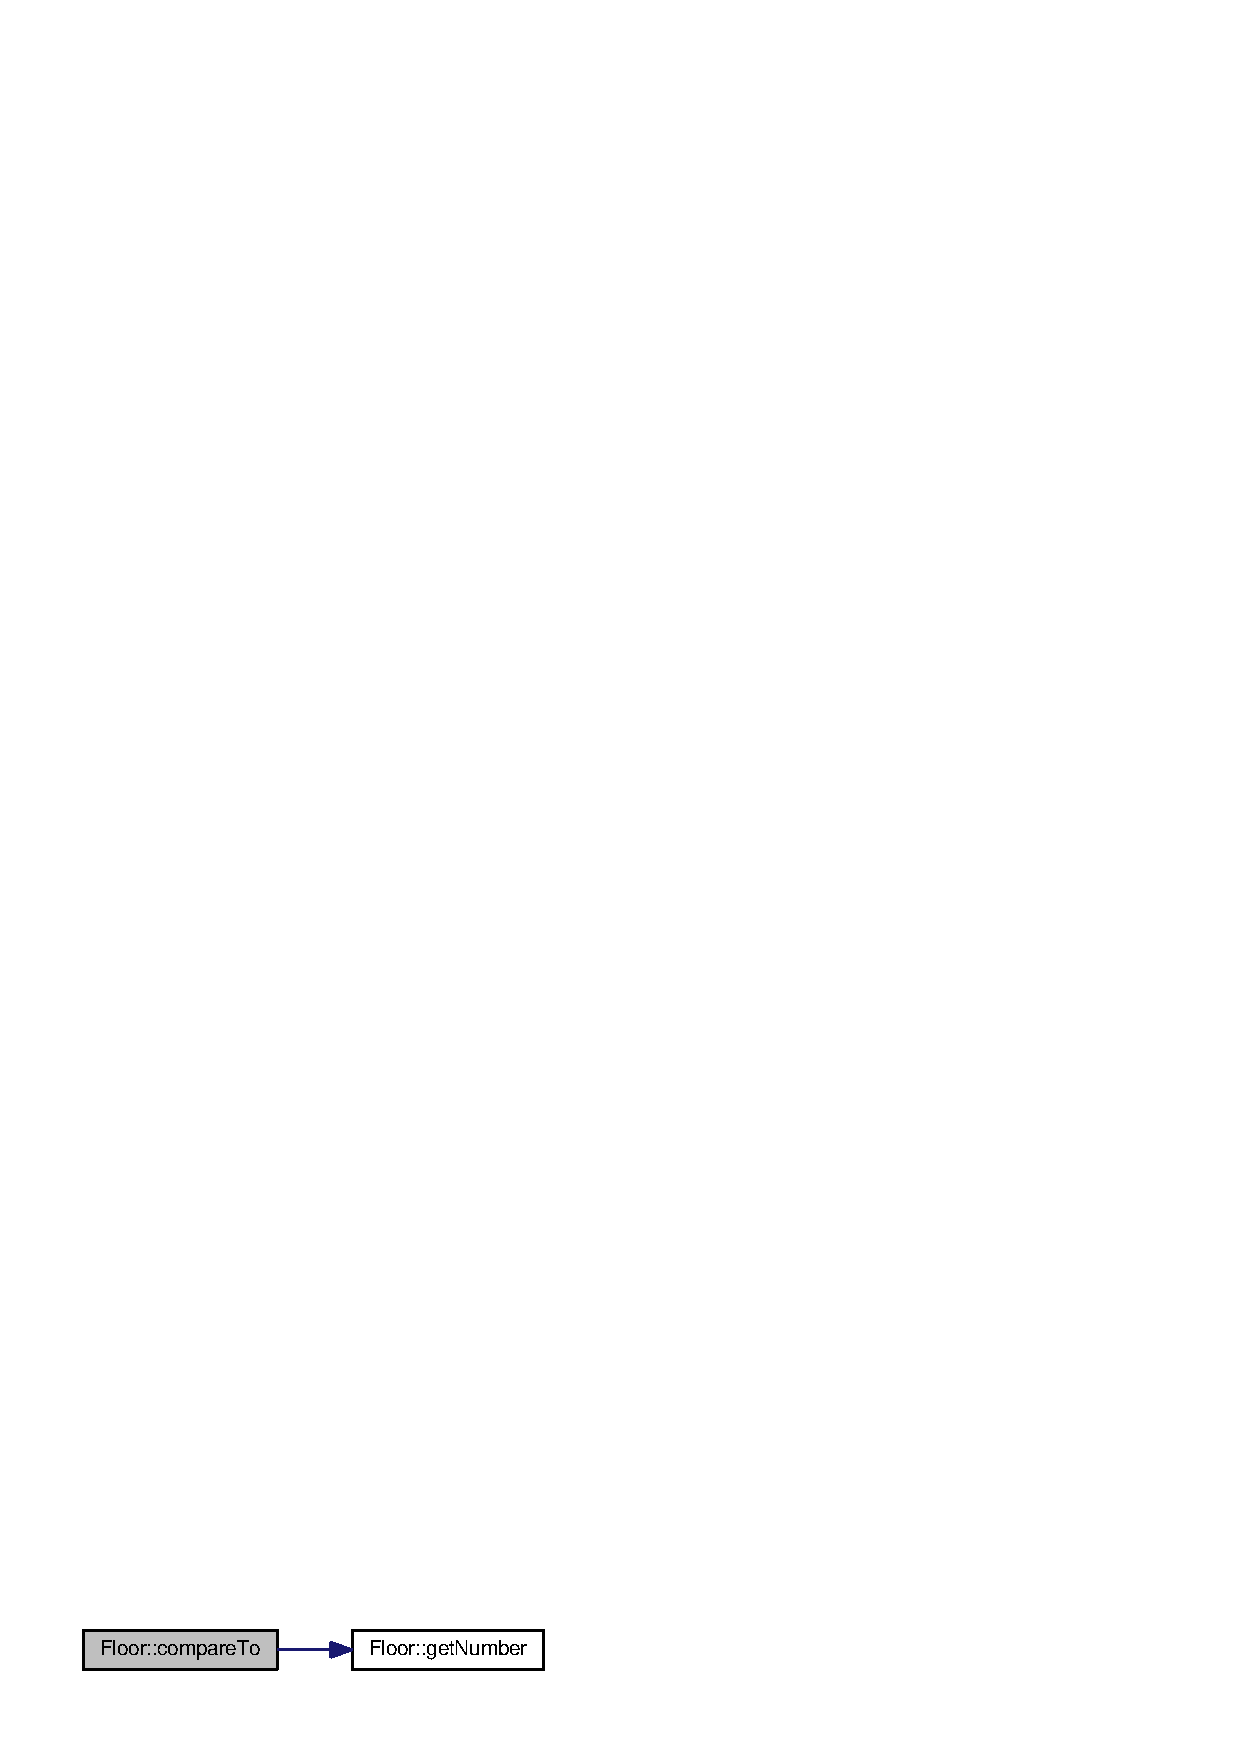
\includegraphics[width=265pt]{class_floor_a09cf6744871fe9b1a1db00d2afa8b723_cgraph}
\end{center}
\end{figure}


\index{Floor@{Floor}!create@{create}}
\index{create@{create}!Floor@{Floor}}
\subsubsection[{create}]{\setlength{\rightskip}{0pt plus 5cm}std\+::shared\+\_\+ptr$<$ std\+::vector$<$ std\+::shared\+\_\+ptr$<$ {\bf Floor} $>$ $>$ $>$ Floor\+::create (
\begin{DoxyParamCaption}
\item[{const std\+::shared\+\_\+ptr$<$ const {\bf Simulator} $>$}]{simulator}
\end{DoxyParamCaption}
)\hspace{0.3cm}{\ttfamily [static]}}\label{class_floor_a294df3a0179a79c3a9a2765418368d03}


Definition at line 149 of file Floor.\+cpp.



Here is the caller graph for this function\+:\nopagebreak
\begin{figure}[H]
\begin{center}
\leavevmode
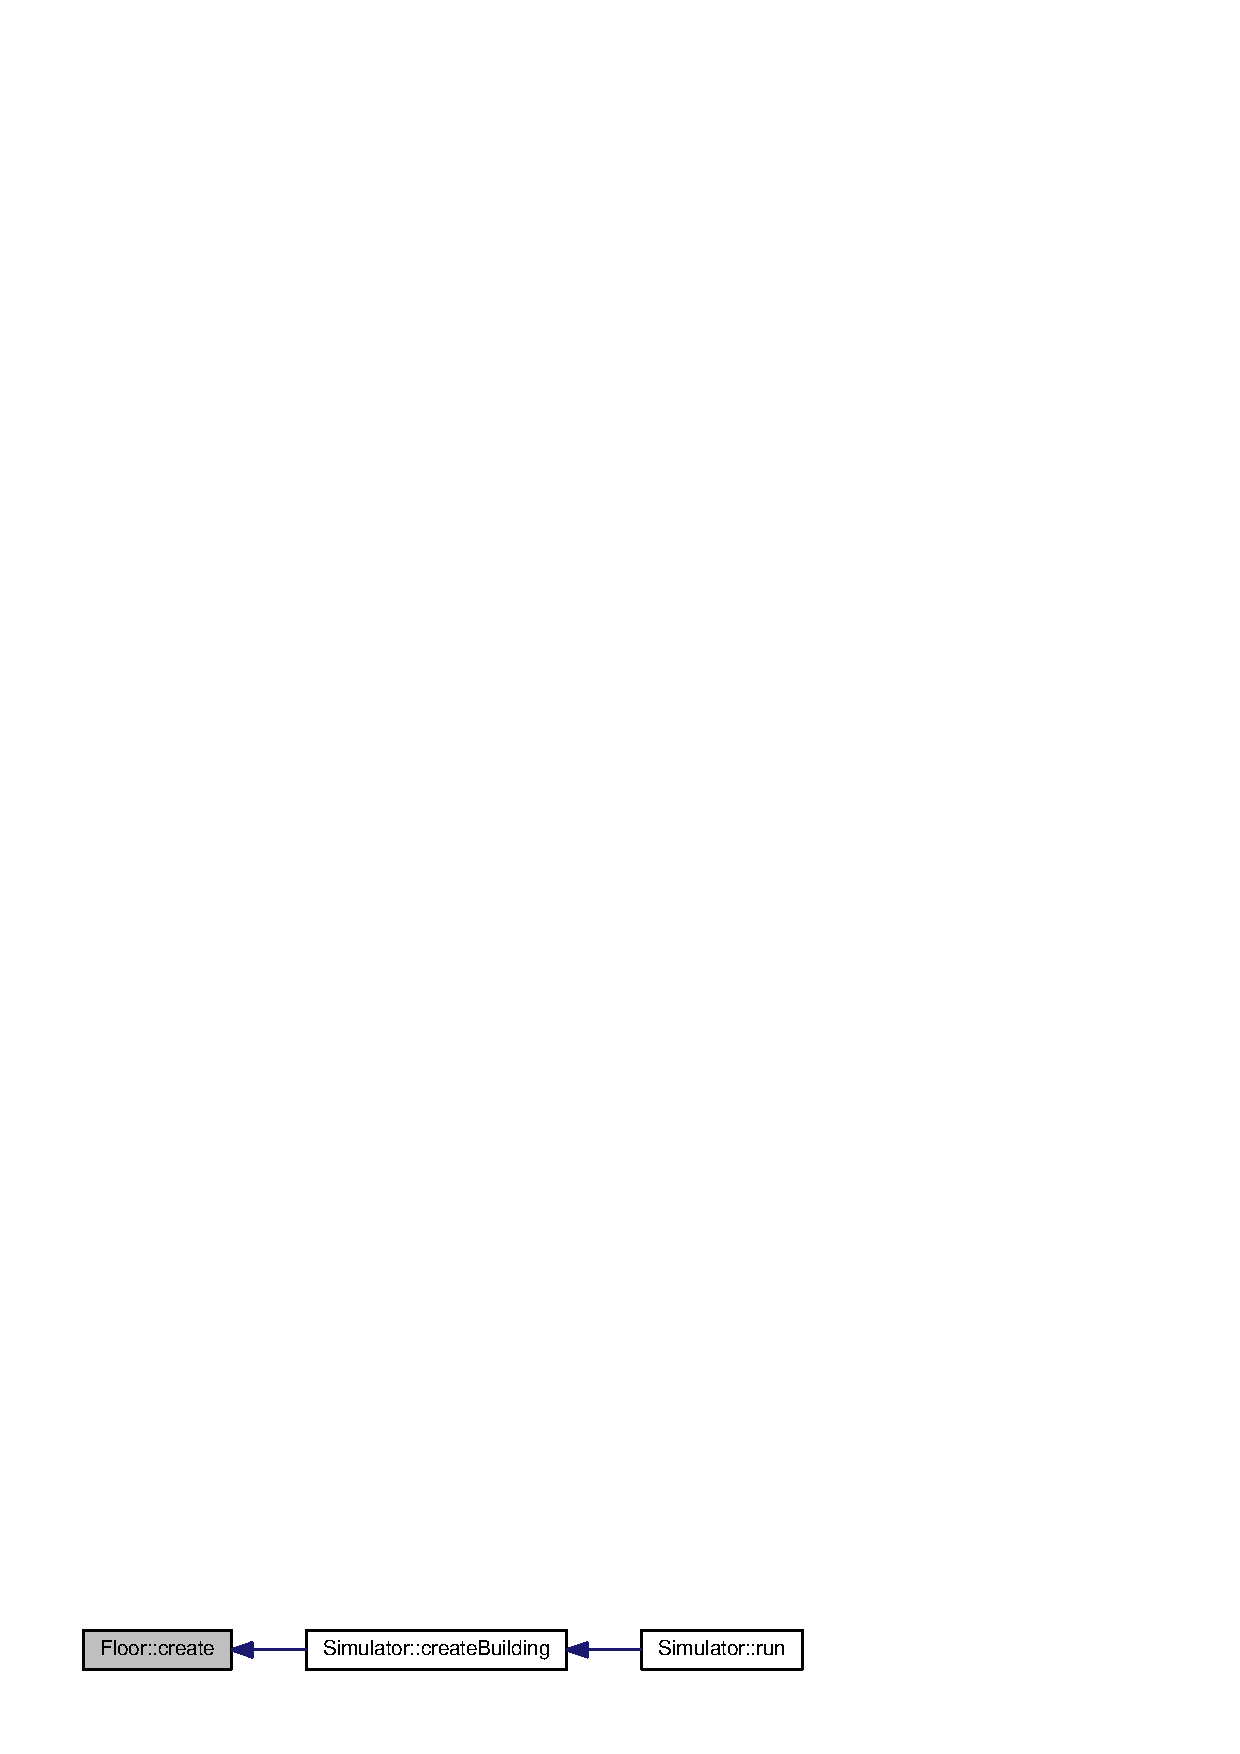
\includegraphics[width=350pt]{class_floor_a294df3a0179a79c3a9a2765418368d03_icgraph}
\end{center}
\end{figure}


\index{Floor@{Floor}!create\+Future\+Arrival@{create\+Future\+Arrival}}
\index{create\+Future\+Arrival@{create\+Future\+Arrival}!Floor@{Floor}}
\subsubsection[{create\+Future\+Arrival}]{\setlength{\rightskip}{0pt plus 5cm}void Floor\+::create\+Future\+Arrival (
\begin{DoxyParamCaption}
\item[{const std\+::shared\+\_\+ptr$<$ {\bf Event\+Queue} $>$}]{event\+Queue}
\end{DoxyParamCaption}
)}\label{class_floor_a92fcea5eb3324a506bfd33be2c292b35}


Definition at line 145 of file Floor.\+cpp.

\index{Floor@{Floor}!get\+Down\+Line@{get\+Down\+Line}}
\index{get\+Down\+Line@{get\+Down\+Line}!Floor@{Floor}}
\subsubsection[{get\+Down\+Line}]{\setlength{\rightskip}{0pt plus 5cm}const std\+::vector$<$ std\+::shared\+\_\+ptr$<$ {\bf Client} $>$ $>$ Floor\+::get\+Down\+Line (
\begin{DoxyParamCaption}
\item[{int}]{n}
\end{DoxyParamCaption}
) const}\label{class_floor_adfe3cef0e8a451e6290bcfdccf2f5350}


Definition at line 65 of file Floor.\+cpp.

\index{Floor@{Floor}!get\+Down\+Line\+Copy@{get\+Down\+Line\+Copy}}
\index{get\+Down\+Line\+Copy@{get\+Down\+Line\+Copy}!Floor@{Floor}}
\subsubsection[{get\+Down\+Line\+Copy}]{\setlength{\rightskip}{0pt plus 5cm}std\+::queue$<$ std\+::shared\+\_\+ptr$<$ {\bf Client} $>$ $>$ Floor\+::get\+Down\+Line\+Copy (
\begin{DoxyParamCaption}
{}
\end{DoxyParamCaption}
) const}\label{class_floor_a34ce9bfe12a7def89a405ed73a3f5655}


Definition at line 42 of file Floor.\+cpp.

\index{Floor@{Floor}!get\+Lambda@{get\+Lambda}}
\index{get\+Lambda@{get\+Lambda}!Floor@{Floor}}
\subsubsection[{get\+Lambda}]{\setlength{\rightskip}{0pt plus 5cm}int Floor\+::get\+Lambda (
\begin{DoxyParamCaption}
{}
\end{DoxyParamCaption}
) const}\label{class_floor_a566668c8b6558cec6a9878043530aa6e}


Definition at line 24 of file Floor.\+cpp.

\index{Floor@{Floor}!get\+Number@{get\+Number}}
\index{get\+Number@{get\+Number}!Floor@{Floor}}
\subsubsection[{get\+Number}]{\setlength{\rightskip}{0pt plus 5cm}int Floor\+::get\+Number (
\begin{DoxyParamCaption}
{}
\end{DoxyParamCaption}
) const}\label{class_floor_a4368d12bf63b63847f5b761c328fd133}


Definition at line 22 of file Floor.\+cpp.



Here is the caller graph for this function\+:\nopagebreak
\begin{figure}[H]
\begin{center}
\leavevmode
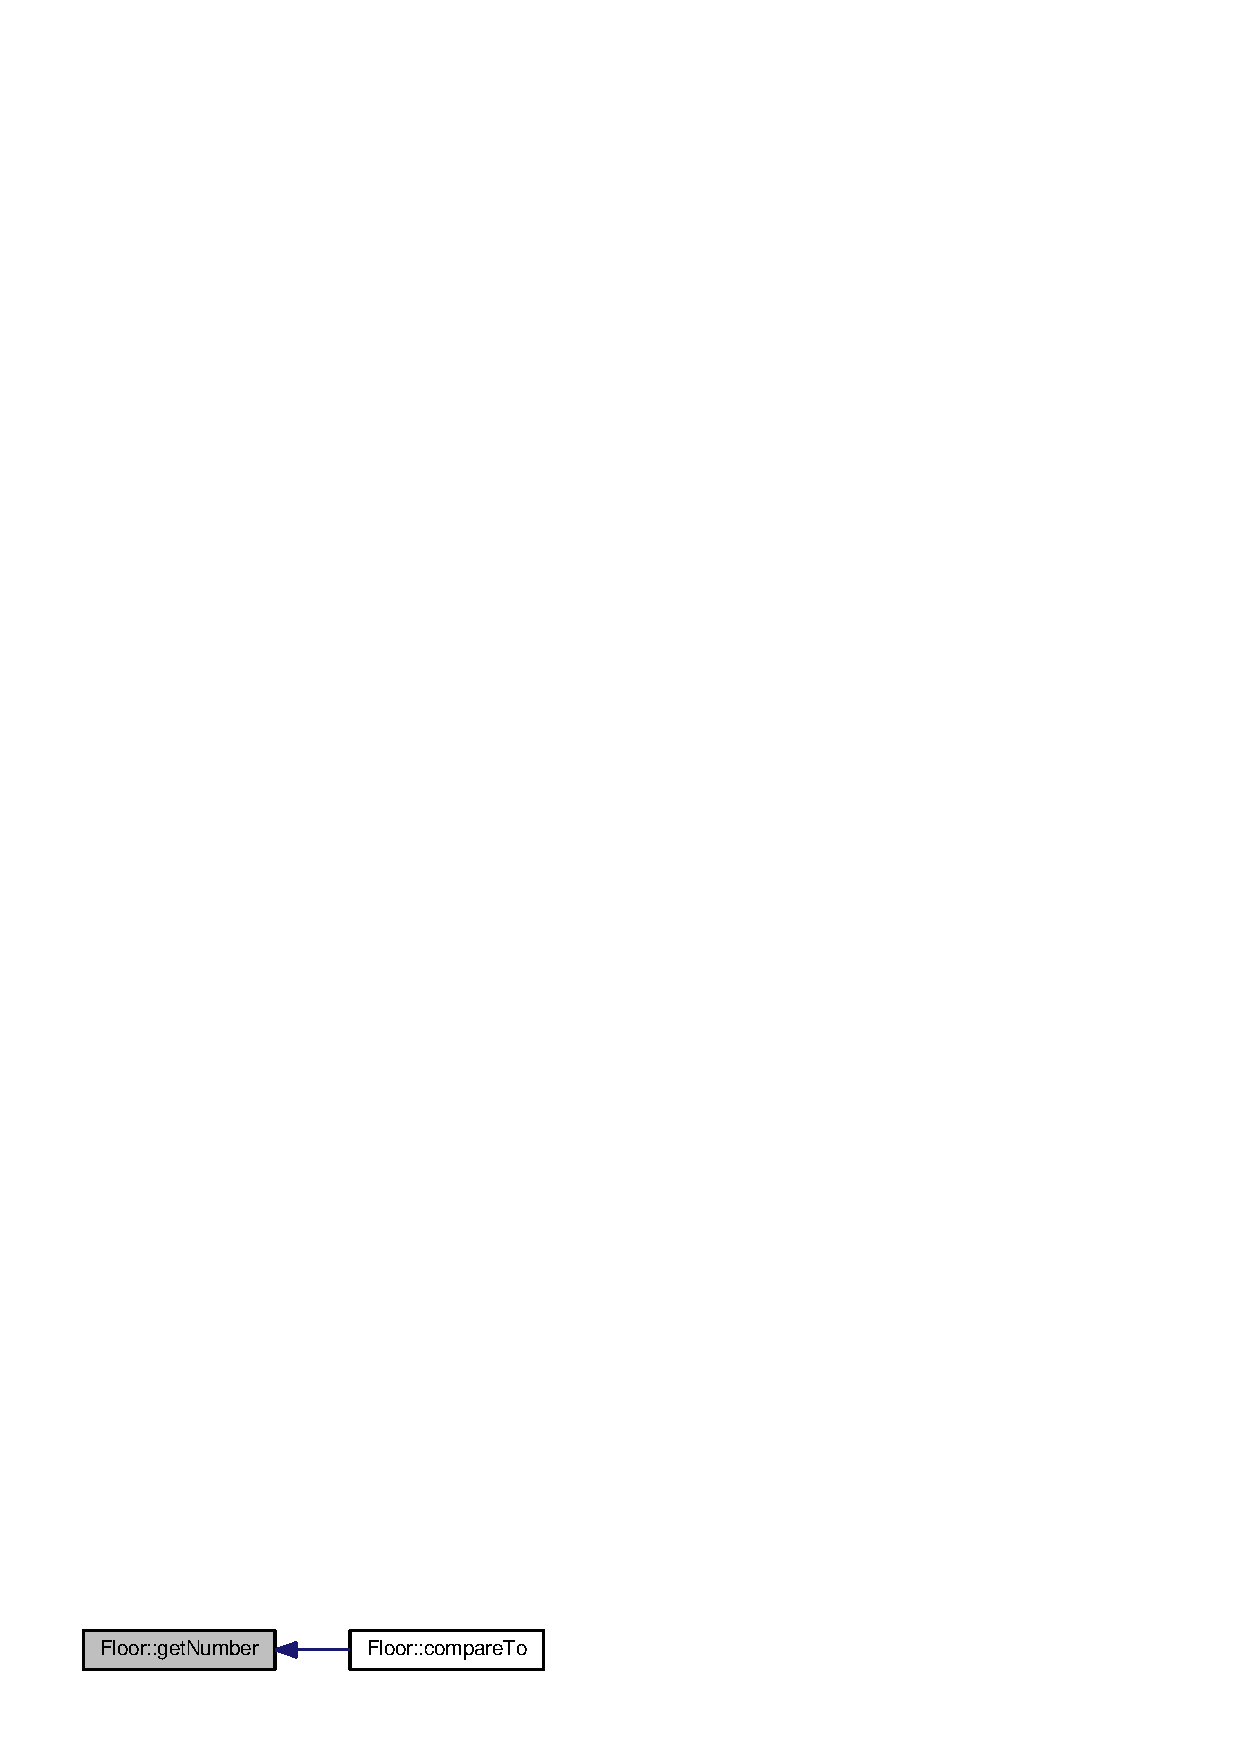
\includegraphics[width=265pt]{class_floor_a4368d12bf63b63847f5b761c328fd133_icgraph}
\end{center}
\end{figure}


\index{Floor@{Floor}!get\+Up\+Line@{get\+Up\+Line}}
\index{get\+Up\+Line@{get\+Up\+Line}!Floor@{Floor}}
\subsubsection[{get\+Up\+Line}]{\setlength{\rightskip}{0pt plus 5cm}const std\+::vector$<$ std\+::shared\+\_\+ptr$<$ {\bf Client} $>$ $>$ Floor\+::get\+Up\+Line (
\begin{DoxyParamCaption}
\item[{int}]{n}
\end{DoxyParamCaption}
) const}\label{class_floor_aa39831329839d4278e812c02f40b75b8}


Definition at line 54 of file Floor.\+cpp.

\index{Floor@{Floor}!get\+Up\+Line\+Copy@{get\+Up\+Line\+Copy}}
\index{get\+Up\+Line\+Copy@{get\+Up\+Line\+Copy}!Floor@{Floor}}
\subsubsection[{get\+Up\+Line\+Copy}]{\setlength{\rightskip}{0pt plus 5cm}std\+::queue$<$ std\+::shared\+\_\+ptr$<$ {\bf Client} $>$ $>$ Floor\+::get\+Up\+Line\+Copy (
\begin{DoxyParamCaption}
{}
\end{DoxyParamCaption}
) const}\label{class_floor_a0897897d4bb4aafc7b6aeb0664bc6e40}


Definition at line 30 of file Floor.\+cpp.

\index{Floor@{Floor}!set\+Event\+Factory@{set\+Event\+Factory}}
\index{set\+Event\+Factory@{set\+Event\+Factory}!Floor@{Floor}}
\subsubsection[{set\+Event\+Factory}]{\setlength{\rightskip}{0pt plus 5cm}void Floor\+::set\+Event\+Factory (
\begin{DoxyParamCaption}
\item[{const std\+::shared\+\_\+ptr$<$ {\bf Event\+Factory} $>$}]{event\+Factory}
\end{DoxyParamCaption}
)}\label{class_floor_a14cef459a7a9ddbdb53070d2f35add7f}


Definition at line 83 of file Floor.\+cpp.

\index{Floor@{Floor}!str@{str}}
\index{str@{str}!Floor@{Floor}}
\subsubsection[{str}]{\setlength{\rightskip}{0pt plus 5cm}std\+::string Floor\+::str (
\begin{DoxyParamCaption}
{}
\end{DoxyParamCaption}
) const}\label{class_floor_a46daff13947cd7b753df0d258ec68bed}


Definition at line 167 of file Floor.\+cpp.



The documentation for this class was generated from the following files\+:\begin{DoxyCompactItemize}
\item 
include/{\bf Floor.\+h}\item 
src/{\bf Floor.\+cpp}\end{DoxyCompactItemize}

\section{Floor\+Comparator Struct Reference}
\label{struct_floor_comparator}\index{Floor\+Comparator@{Floor\+Comparator}}


{\ttfamily \#include $<$Stop\+Manager.\+h$>$}



Collaboration diagram for Floor\+Comparator\+:
\nopagebreak
\begin{figure}[H]
\begin{center}
\leavevmode
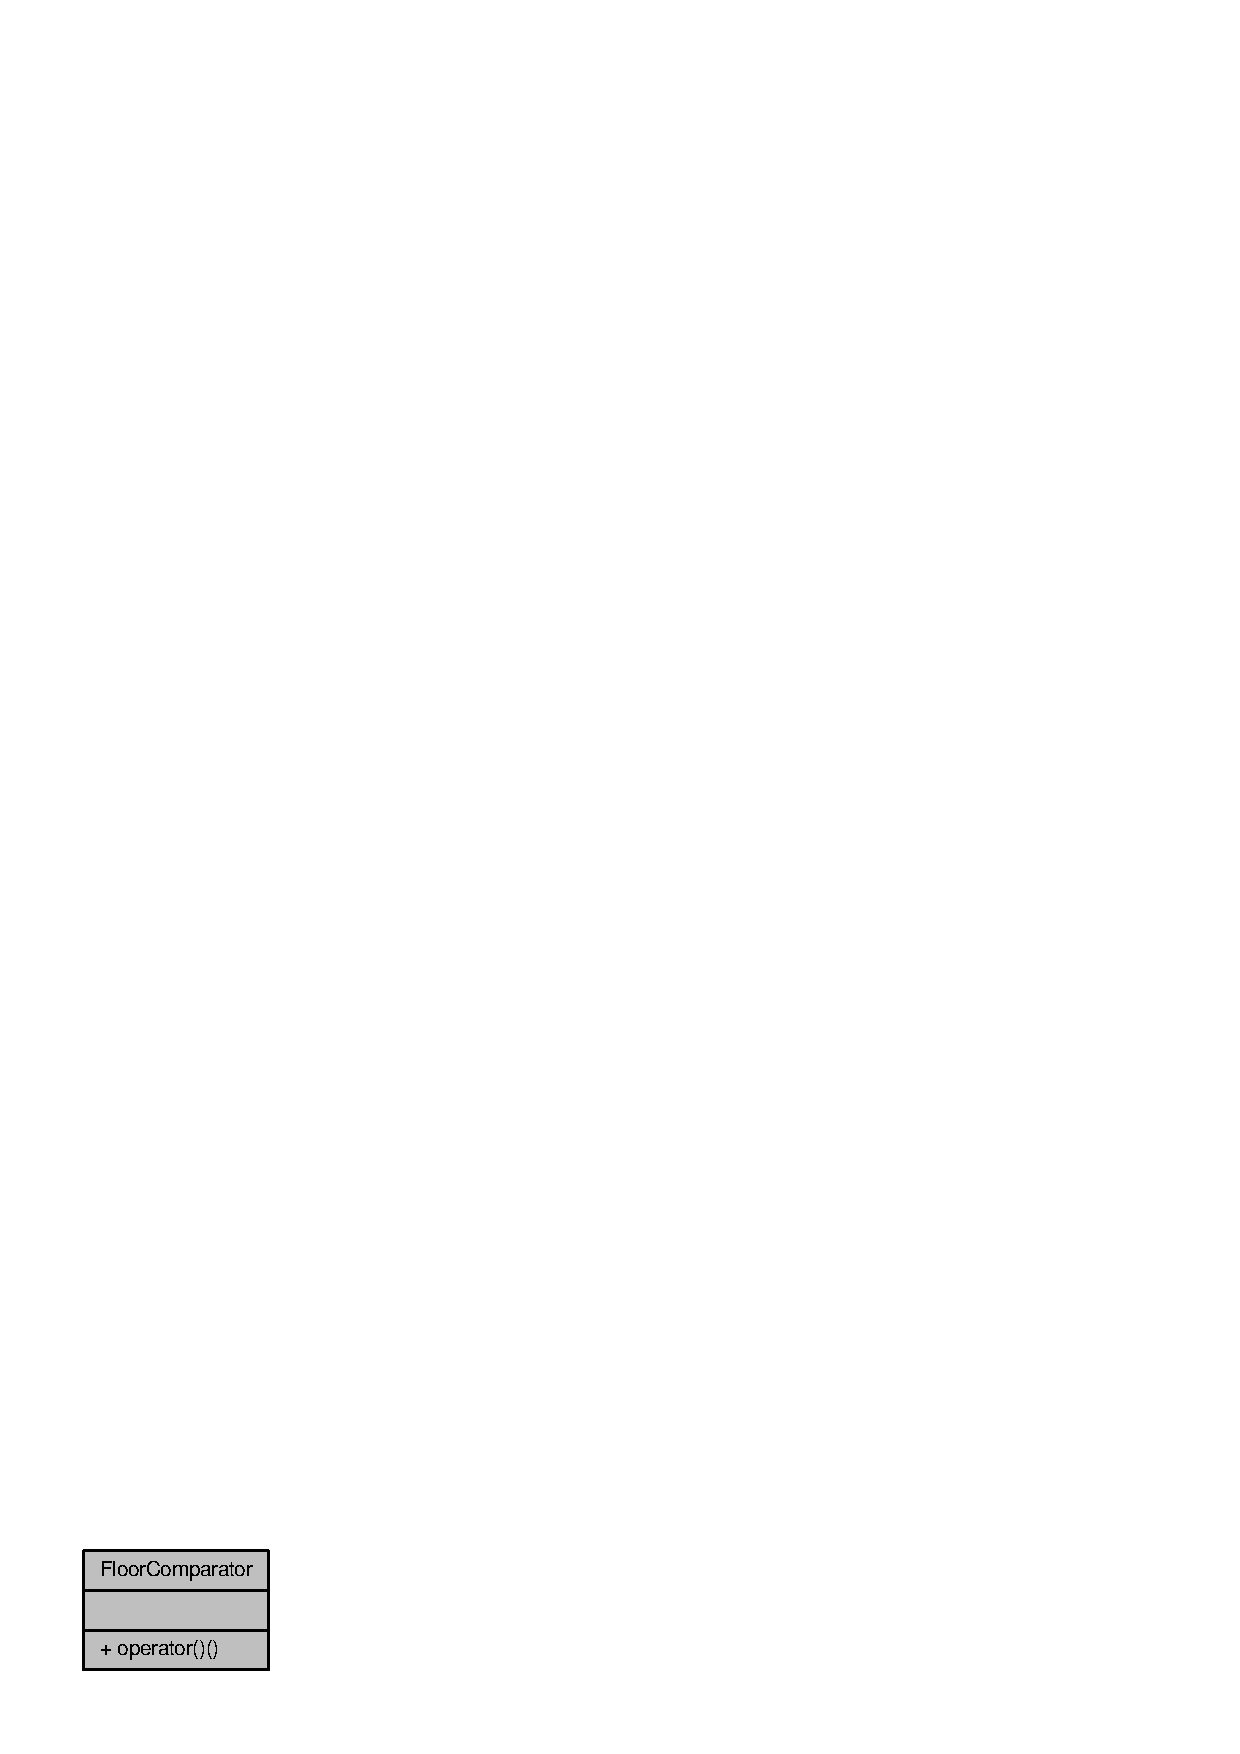
\includegraphics[width=133pt]{struct_floor_comparator__coll__graph}
\end{center}
\end{figure}
\subsection*{Public Member Functions}
\begin{DoxyCompactItemize}
\item 
bool {\bf operator()} (const std\+::shared\+\_\+ptr$<$ {\bf Floor} $>$ \&lhs, const std\+::shared\+\_\+ptr$<$ {\bf Floor} $>$ \&rhs) const 
\end{DoxyCompactItemize}


\subsection{Detailed Description}


Definition at line 11 of file Stop\+Manager.\+h.



\subsection{Member Function Documentation}
\index{Floor\+Comparator@{Floor\+Comparator}!operator()@{operator()}}
\index{operator()@{operator()}!Floor\+Comparator@{Floor\+Comparator}}
\subsubsection[{operator()}]{\setlength{\rightskip}{0pt plus 5cm}bool Floor\+Comparator\+::operator() (
\begin{DoxyParamCaption}
\item[{const std\+::shared\+\_\+ptr$<$ {\bf Floor} $>$ \&}]{lhs, }
\item[{const std\+::shared\+\_\+ptr$<$ {\bf Floor} $>$ \&}]{rhs}
\end{DoxyParamCaption}
) const\hspace{0.3cm}{\ttfamily [inline]}}\label{struct_floor_comparator_af5dae214e942b08f8f40f29b67deb822}


Definition at line 12 of file Stop\+Manager.\+h.



The documentation for this struct was generated from the following file\+:\begin{DoxyCompactItemize}
\item 
include/{\bf Stop\+Manager.\+h}\end{DoxyCompactItemize}

\section{Missing\+Cost\+Function\+Error Class Reference}
\label{class_missing_cost_function_error}\index{Missing\+Cost\+Function\+Error@{Missing\+Cost\+Function\+Error}}


{\ttfamily \#include $<$Missing\+Cost\+Function\+Error.\+h$>$}



Inheritance diagram for Missing\+Cost\+Function\+Error\+:
\nopagebreak
\begin{figure}[H]
\begin{center}
\leavevmode
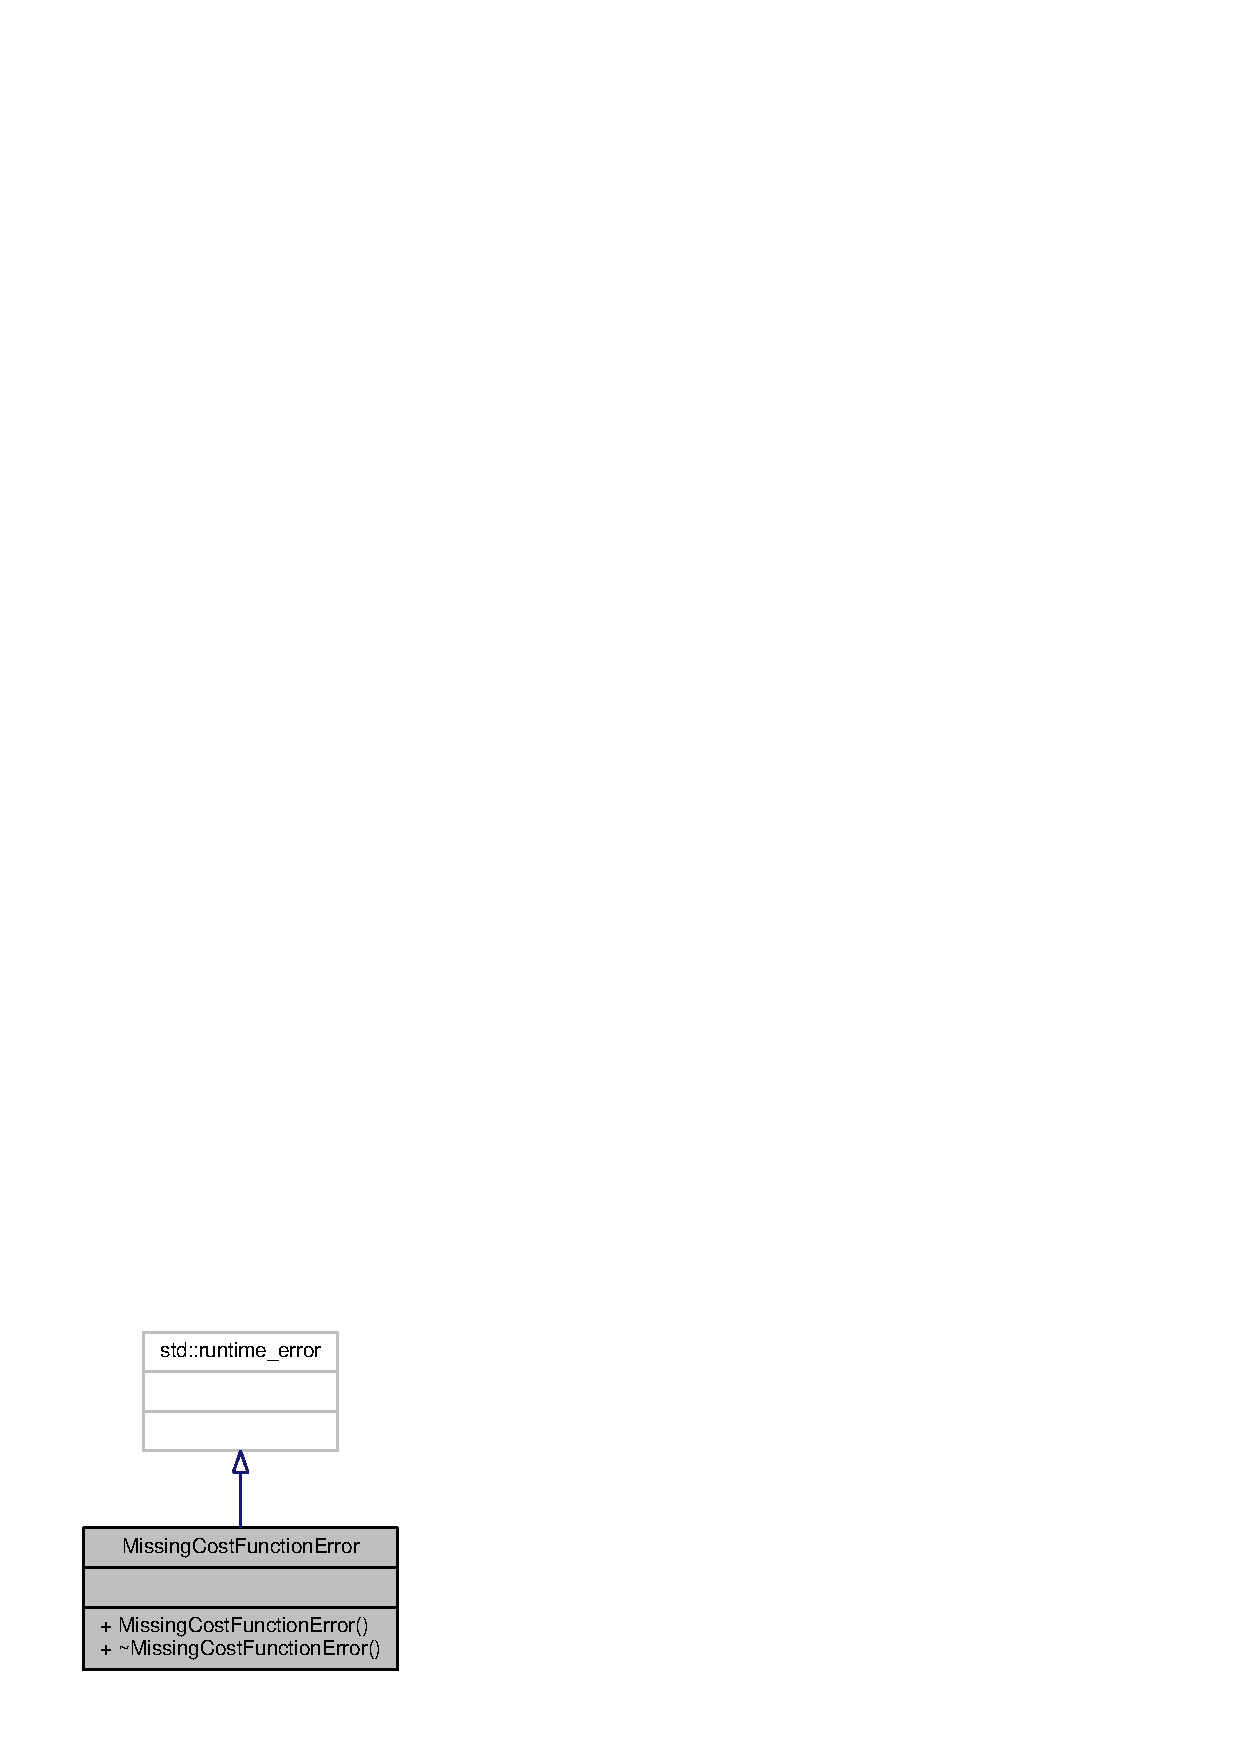
\includegraphics[width=195pt]{class_missing_cost_function_error__inherit__graph}
\end{center}
\end{figure}


Collaboration diagram for Missing\+Cost\+Function\+Error\+:
\nopagebreak
\begin{figure}[H]
\begin{center}
\leavevmode
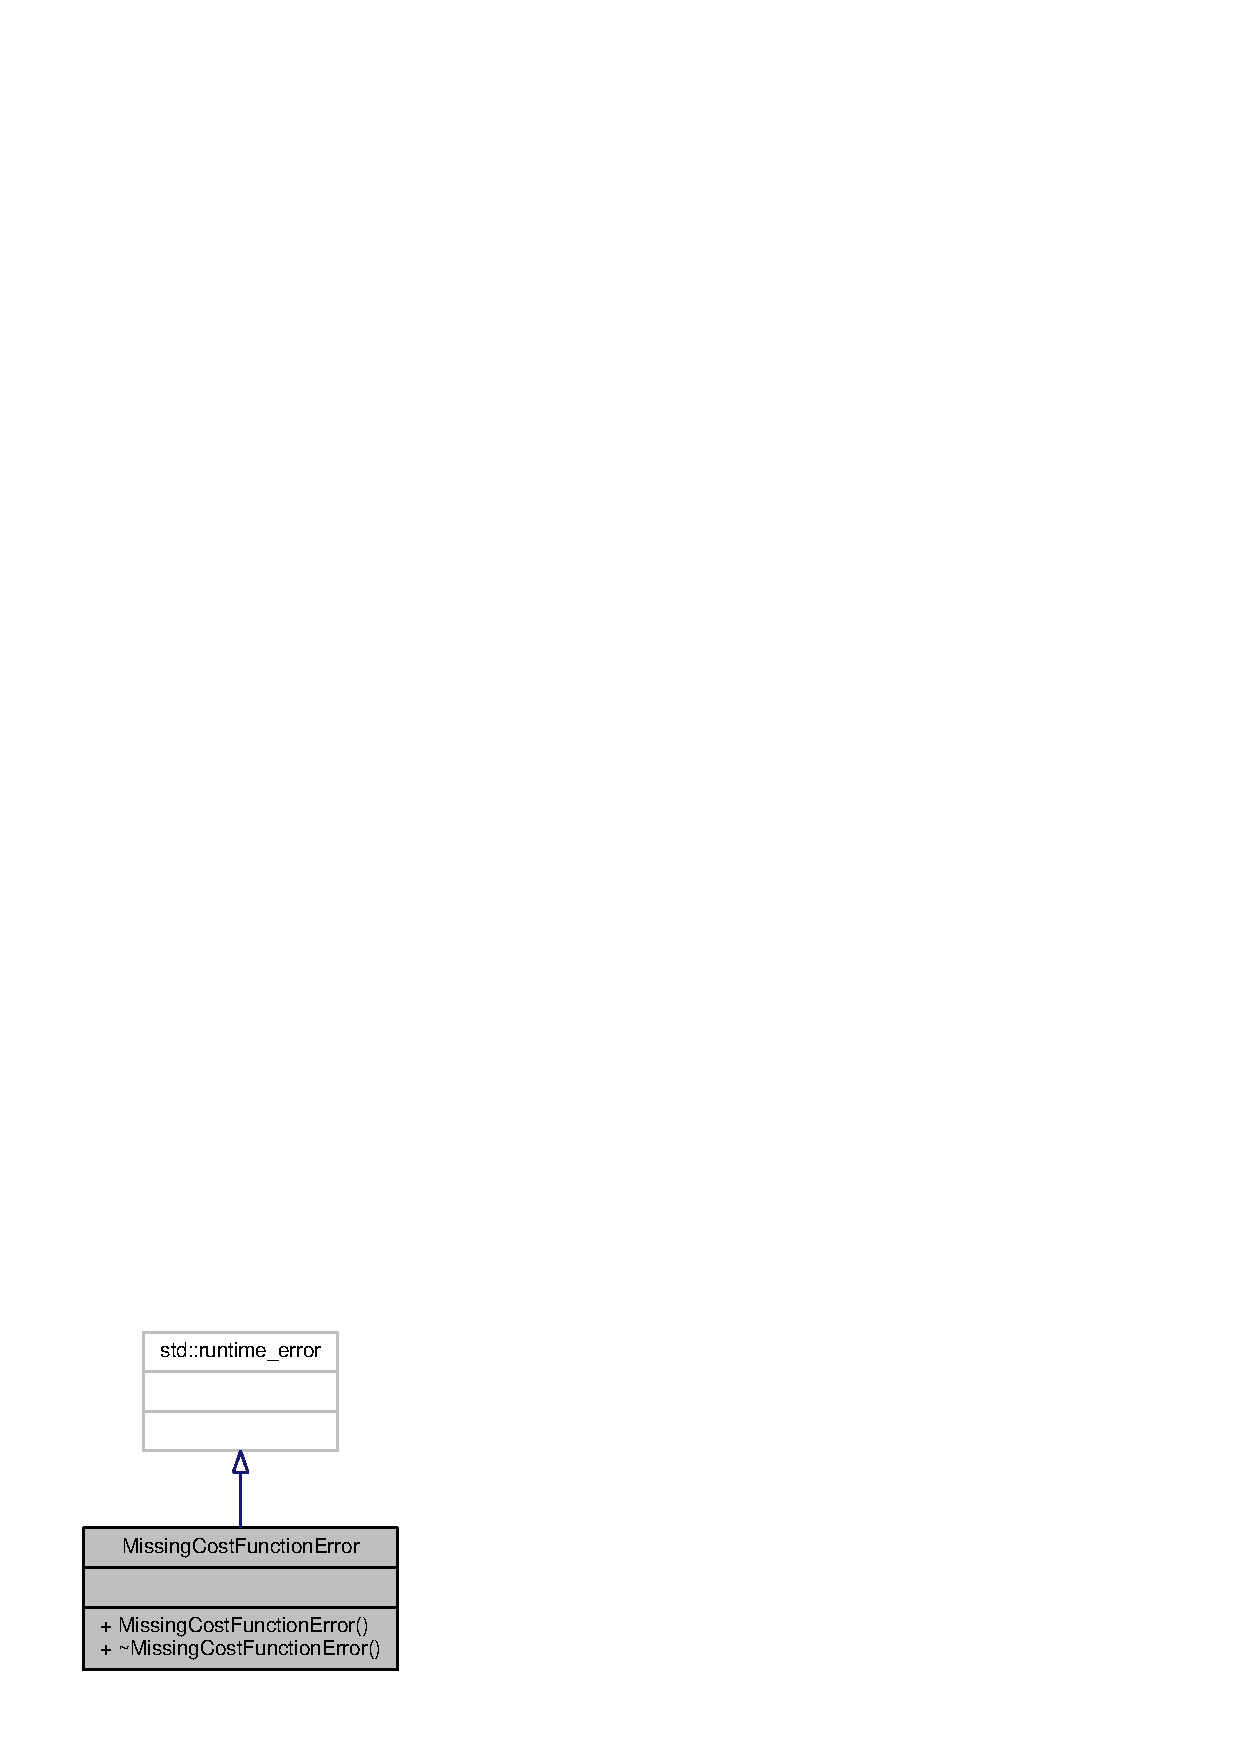
\includegraphics[width=195pt]{class_missing_cost_function_error__coll__graph}
\end{center}
\end{figure}
\subsection*{Public Member Functions}
\begin{DoxyCompactItemize}
\item 
{\bf Missing\+Cost\+Function\+Error} (const std\+::string \&what)
\item 
virtual {\bf $\sim$\+Missing\+Cost\+Function\+Error} ()
\end{DoxyCompactItemize}


\subsection{Detailed Description}


Definition at line 4 of file Missing\+Cost\+Function\+Error.\+h.



\subsection{Constructor \& Destructor Documentation}
\index{Missing\+Cost\+Function\+Error@{Missing\+Cost\+Function\+Error}!Missing\+Cost\+Function\+Error@{Missing\+Cost\+Function\+Error}}
\index{Missing\+Cost\+Function\+Error@{Missing\+Cost\+Function\+Error}!Missing\+Cost\+Function\+Error@{Missing\+Cost\+Function\+Error}}
\subsubsection[{Missing\+Cost\+Function\+Error}]{\setlength{\rightskip}{0pt plus 5cm}Missing\+Cost\+Function\+Error\+::\+Missing\+Cost\+Function\+Error (
\begin{DoxyParamCaption}
\item[{const std\+::string \&}]{what}
\end{DoxyParamCaption}
)\hspace{0.3cm}{\ttfamily [inline]}, {\ttfamily [explicit]}}\label{class_missing_cost_function_error_a0b7c5e482aa0b2a713ea9a46975244ba}


Definition at line 6 of file Missing\+Cost\+Function\+Error.\+h.

\index{Missing\+Cost\+Function\+Error@{Missing\+Cost\+Function\+Error}!````~Missing\+Cost\+Function\+Error@{$\sim$\+Missing\+Cost\+Function\+Error}}
\index{````~Missing\+Cost\+Function\+Error@{$\sim$\+Missing\+Cost\+Function\+Error}!Missing\+Cost\+Function\+Error@{Missing\+Cost\+Function\+Error}}
\subsubsection[{$\sim$\+Missing\+Cost\+Function\+Error}]{\setlength{\rightskip}{0pt plus 5cm}virtual Missing\+Cost\+Function\+Error\+::$\sim$\+Missing\+Cost\+Function\+Error (
\begin{DoxyParamCaption}
{}
\end{DoxyParamCaption}
)\hspace{0.3cm}{\ttfamily [inline]}, {\ttfamily [virtual]}}\label{class_missing_cost_function_error_a1e51bbbb052d985f514b8265a8bf0846}


Definition at line 8 of file Missing\+Cost\+Function\+Error.\+h.



The documentation for this class was generated from the following file\+:\begin{DoxyCompactItemize}
\item 
include/{\bf Missing\+Cost\+Function\+Error.\+h}\end{DoxyCompactItemize}

\section{Missing\+Scheduler\+Error Class Reference}
\label{class_missing_scheduler_error}\index{Missing\+Scheduler\+Error@{Missing\+Scheduler\+Error}}


{\ttfamily \#include $<$Missing\+Scheduler\+Error.\+h$>$}



Inheritance diagram for Missing\+Scheduler\+Error\+:\nopagebreak
\begin{figure}[H]
\begin{center}
\leavevmode
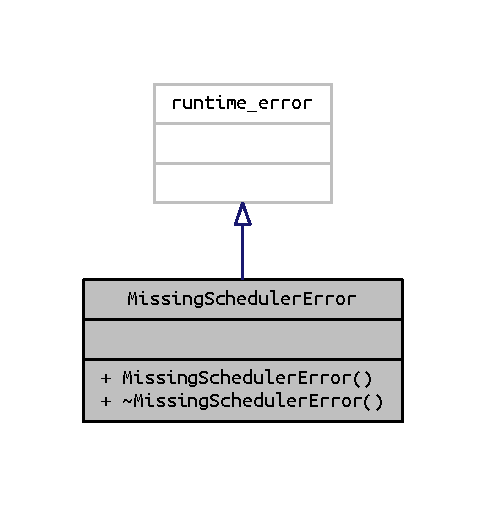
\includegraphics[width=180pt]{class_missing_scheduler_error__inherit__graph}
\end{center}
\end{figure}


Collaboration diagram for Missing\+Scheduler\+Error\+:\nopagebreak
\begin{figure}[H]
\begin{center}
\leavevmode
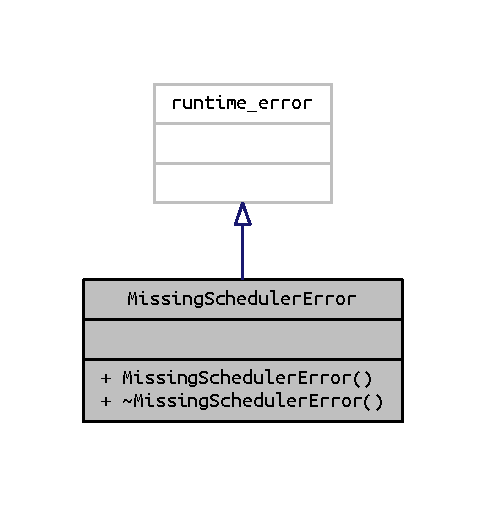
\includegraphics[width=180pt]{class_missing_scheduler_error__coll__graph}
\end{center}
\end{figure}
\subsection*{Public Member Functions}
\begin{DoxyCompactItemize}
\item 
{\bf Missing\+Scheduler\+Error} (const std\+::string \&what)
\item 
virtual {\bf $\sim$\+Missing\+Scheduler\+Error} ()
\end{DoxyCompactItemize}


\subsection{Detailed Description}


Definition at line 4 of file Missing\+Scheduler\+Error.\+h.



\subsection{Constructor \& Destructor Documentation}
\index{Missing\+Scheduler\+Error@{Missing\+Scheduler\+Error}!Missing\+Scheduler\+Error@{Missing\+Scheduler\+Error}}
\index{Missing\+Scheduler\+Error@{Missing\+Scheduler\+Error}!Missing\+Scheduler\+Error@{Missing\+Scheduler\+Error}}
\subsubsection[{Missing\+Scheduler\+Error}]{\setlength{\rightskip}{0pt plus 5cm}Missing\+Scheduler\+Error\+::\+Missing\+Scheduler\+Error (
\begin{DoxyParamCaption}
\item[{const std\+::string \&}]{what}
\end{DoxyParamCaption}
)\hspace{0.3cm}{\ttfamily [inline]}, {\ttfamily [explicit]}}\label{class_missing_scheduler_error_a381df77f3b4c59a056fa31c4c2d567d9}


Definition at line 6 of file Missing\+Scheduler\+Error.\+h.

\index{Missing\+Scheduler\+Error@{Missing\+Scheduler\+Error}!````~Missing\+Scheduler\+Error@{$\sim$\+Missing\+Scheduler\+Error}}
\index{````~Missing\+Scheduler\+Error@{$\sim$\+Missing\+Scheduler\+Error}!Missing\+Scheduler\+Error@{Missing\+Scheduler\+Error}}
\subsubsection[{$\sim$\+Missing\+Scheduler\+Error}]{\setlength{\rightskip}{0pt plus 5cm}virtual Missing\+Scheduler\+Error\+::$\sim$\+Missing\+Scheduler\+Error (
\begin{DoxyParamCaption}
{}
\end{DoxyParamCaption}
)\hspace{0.3cm}{\ttfamily [inline]}, {\ttfamily [virtual]}}\label{class_missing_scheduler_error_aac5812e2334a64d734a73e3e0304f1ca}


Definition at line 8 of file Missing\+Scheduler\+Error.\+h.



The documentation for this class was generated from the following file\+:\begin{DoxyCompactItemize}
\item 
include/{\bf Missing\+Scheduler\+Error.\+h}\end{DoxyCompactItemize}

\section{Nearest\+Neighbour\+Cost\+Function Class Reference}
\label{class_nearest_neighbour_cost_function}\index{Nearest\+Neighbour\+Cost\+Function@{Nearest\+Neighbour\+Cost\+Function}}


{\ttfamily \#include $<$Nearest\+Neighbour\+Cost\+Function.\+h$>$}



Inheritance diagram for Nearest\+Neighbour\+Cost\+Function\+:\nopagebreak
\begin{figure}[H]
\begin{center}
\leavevmode
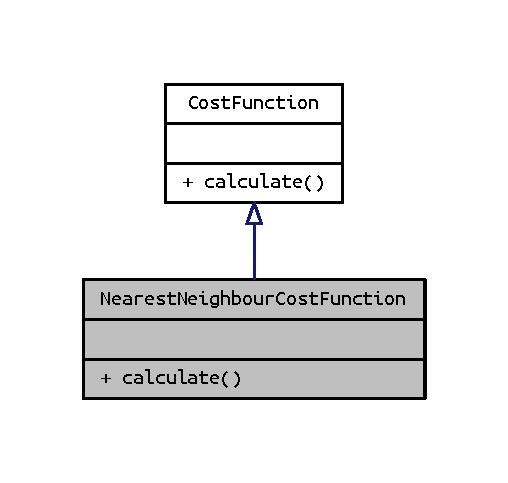
\includegraphics[width=198pt]{class_nearest_neighbour_cost_function__inherit__graph}
\end{center}
\end{figure}


Collaboration diagram for Nearest\+Neighbour\+Cost\+Function\+:\nopagebreak
\begin{figure}[H]
\begin{center}
\leavevmode
\includegraphics[width=198pt]{class_nearest_neighbour_cost_function__coll__graph}
\end{center}
\end{figure}
\subsection*{Public Member Functions}
\begin{DoxyCompactItemize}
\item 
float {\bf calculate} (const std\+::shared\+\_\+ptr$<$ const {\bf Building} $>$ building, const std\+::shared\+\_\+ptr$<$ const {\bf Elevator} $>$ elevator, const std\+::shared\+\_\+ptr$<$ const {\bf Client} $>$ client)
\end{DoxyCompactItemize}


\subsection{Detailed Description}


Definition at line 9 of file Nearest\+Neighbour\+Cost\+Function.\+h.



\subsection{Member Function Documentation}
\index{Nearest\+Neighbour\+Cost\+Function@{Nearest\+Neighbour\+Cost\+Function}!calculate@{calculate}}
\index{calculate@{calculate}!Nearest\+Neighbour\+Cost\+Function@{Nearest\+Neighbour\+Cost\+Function}}
\subsubsection[{calculate}]{\setlength{\rightskip}{0pt plus 5cm}float Nearest\+Neighbour\+Cost\+Function\+::calculate (
\begin{DoxyParamCaption}
\item[{const std\+::shared\+\_\+ptr$<$ const {\bf Building} $>$}]{building, }
\item[{const std\+::shared\+\_\+ptr$<$ const {\bf Elevator} $>$}]{elevator, }
\item[{const std\+::shared\+\_\+ptr$<$ const {\bf Client} $>$}]{client}
\end{DoxyParamCaption}
)\hspace{0.3cm}{\ttfamily [virtual]}}\label{class_nearest_neighbour_cost_function_ab96d06d3bcd0f3cc56da5928d014c40e}


Implements {\bf Cost\+Function} \doxyref{}{p.}{class_cost_function_ada1a1003e80f4f0e57b20d9a1e6a51c6}.



Definition at line 7 of file Nearest\+Neighbour\+Cost\+Function.\+cpp.



The documentation for this class was generated from the following files\+:\begin{DoxyCompactItemize}
\item 
include/{\bf Nearest\+Neighbour\+Cost\+Function.\+h}\item 
src/{\bf Nearest\+Neighbour\+Cost\+Function.\+cpp}\end{DoxyCompactItemize}

\hypertarget{class_planning_scheduler}{}\section{Planning\+Scheduler Class Reference}
\label{class_planning_scheduler}\index{Planning\+Scheduler@{Planning\+Scheduler}}


{\ttfamily \#include $<$Planning\+Scheduler.\+h$>$}



Inheritance diagram for Planning\+Scheduler\+:
\nopagebreak
\begin{figure}[H]
\begin{center}
\leavevmode
\includegraphics[width=228pt]{class_planning_scheduler__inherit__graph}
\end{center}
\end{figure}


Collaboration diagram for Planning\+Scheduler\+:
\nopagebreak
\begin{figure}[H]
\begin{center}
\leavevmode
\includegraphics[width=228pt]{class_planning_scheduler__coll__graph}
\end{center}
\end{figure}
\subsection*{Public Member Functions}
\begin{DoxyCompactItemize}
\item 
int \hyperlink{class_planning_scheduler_a30e0bb81405e162e596e428cb2a6c1e3}{schedule} (const std\+::shared\+\_\+ptr$<$ \hyperlink{class_cost_function}{Cost\+Function} $>$ cost\+Function, const std\+::shared\+\_\+ptr$<$ const \hyperlink{class_building}{Building} $>$ building, const std\+::shared\+\_\+ptr$<$ const \hyperlink{class_client}{Client} $>$ client, const int elevator\+To\+Exclude=-\/1)
\end{DoxyCompactItemize}
\subsection*{Additional Inherited Members}


\subsection{Member Function Documentation}
\hypertarget{class_planning_scheduler_a30e0bb81405e162e596e428cb2a6c1e3}{}\index{Planning\+Scheduler@{Planning\+Scheduler}!schedule@{schedule}}
\index{schedule@{schedule}!Planning\+Scheduler@{Planning\+Scheduler}}
\subsubsection[{schedule}]{\setlength{\rightskip}{0pt plus 5cm}int Planning\+Scheduler\+::schedule (
\begin{DoxyParamCaption}
\item[{const std\+::shared\+\_\+ptr$<$ {\bf Cost\+Function} $>$}]{cost\+Function, }
\item[{const std\+::shared\+\_\+ptr$<$ const {\bf Building} $>$}]{building, }
\item[{const std\+::shared\+\_\+ptr$<$ const {\bf Client} $>$}]{client, }
\item[{const int}]{elevator\+To\+Exclude = {\ttfamily -\/1}}
\end{DoxyParamCaption}
)\hspace{0.3cm}{\ttfamily [virtual]}}\label{class_planning_scheduler_a30e0bb81405e162e596e428cb2a6c1e3}


Implements \hyperlink{class_scheduler_aabaa3785dd1aa6efcf407a1e027cfced}{Scheduler}.



Here is the call graph for this function\+:
\nopagebreak
\begin{figure}[H]
\begin{center}
\leavevmode
\includegraphics[width=350pt]{class_planning_scheduler_a30e0bb81405e162e596e428cb2a6c1e3_cgraph}
\end{center}
\end{figure}




The documentation for this class was generated from the following files\+:\begin{DoxyCompactItemize}
\item 
include/\hyperlink{_planning_scheduler_8h}{Planning\+Scheduler.\+h}\item 
src/\hyperlink{_planning_scheduler_8cpp}{Planning\+Scheduler.\+cpp}\end{DoxyCompactItemize}

\section{Random\+Cost\+Function Class Reference}
\label{class_random_cost_function}\index{Random\+Cost\+Function@{Random\+Cost\+Function}}


{\ttfamily \#include $<$Random\+Cost\+Function.\+h$>$}



Inheritance diagram for Random\+Cost\+Function\+:
\nopagebreak
\begin{figure}[H]
\begin{center}
\leavevmode
\includegraphics[width=171pt]{class_random_cost_function__inherit__graph}
\end{center}
\end{figure}


Collaboration diagram for Random\+Cost\+Function\+:
\nopagebreak
\begin{figure}[H]
\begin{center}
\leavevmode
\includegraphics[width=171pt]{class_random_cost_function__coll__graph}
\end{center}
\end{figure}
\subsection*{Public Member Functions}
\begin{DoxyCompactItemize}
\item 
{\bf Random\+Cost\+Function} ()
\item 
float {\bf calculate} (const std\+::shared\+\_\+ptr$<$ const {\bf Building} $>$ building, const std\+::shared\+\_\+ptr$<$ const {\bf Elevator} $>$ elevator, const std\+::shared\+\_\+ptr$<$ const {\bf Client} $>$ client)
\end{DoxyCompactItemize}


\subsection{Detailed Description}


Definition at line 13 of file Random\+Cost\+Function.\+h.



\subsection{Constructor \& Destructor Documentation}
\index{Random\+Cost\+Function@{Random\+Cost\+Function}!Random\+Cost\+Function@{Random\+Cost\+Function}}
\index{Random\+Cost\+Function@{Random\+Cost\+Function}!Random\+Cost\+Function@{Random\+Cost\+Function}}
\subsubsection[{Random\+Cost\+Function}]{\setlength{\rightskip}{0pt plus 5cm}Random\+Cost\+Function\+::\+Random\+Cost\+Function (
\begin{DoxyParamCaption}
{}
\end{DoxyParamCaption}
)}\label{class_random_cost_function_ae07362ac36bce45b2e8ff08077f058af}


Definition at line 3 of file Random\+Cost\+Function.\+cpp.



\subsection{Member Function Documentation}
\index{Random\+Cost\+Function@{Random\+Cost\+Function}!calculate@{calculate}}
\index{calculate@{calculate}!Random\+Cost\+Function@{Random\+Cost\+Function}}
\subsubsection[{calculate}]{\setlength{\rightskip}{0pt plus 5cm}float Random\+Cost\+Function\+::calculate (
\begin{DoxyParamCaption}
\item[{const std\+::shared\+\_\+ptr$<$ const {\bf Building} $>$}]{building, }
\item[{const std\+::shared\+\_\+ptr$<$ const {\bf Elevator} $>$}]{elevator, }
\item[{const std\+::shared\+\_\+ptr$<$ const {\bf Client} $>$}]{client}
\end{DoxyParamCaption}
)\hspace{0.3cm}{\ttfamily [virtual]}}\label{class_random_cost_function_a19c472a58df16e9805af2dfba3462fd9}


Implements {\bf Cost\+Function} \doxyref{}{p.}{class_cost_function_ada1a1003e80f4f0e57b20d9a1e6a51c6}.



Definition at line 10 of file Random\+Cost\+Function.\+cpp.



The documentation for this class was generated from the following files\+:\begin{DoxyCompactItemize}
\item 
include/{\bf Random\+Cost\+Function.\+h}\item 
src/{\bf Random\+Cost\+Function.\+cpp}\end{DoxyCompactItemize}

\section{Reporter Class Reference}
\label{class_reporter}\index{Reporter@{Reporter}}


{\ttfamily \#include $<$Reporter.\+h$>$}



Collaboration diagram for Reporter\+:\nopagebreak
\begin{figure}[H]
\begin{center}
\leavevmode
\includegraphics[width=173pt]{class_reporter__coll__graph}
\end{center}
\end{figure}
\subsection*{Public Member Functions}
\begin{DoxyCompactItemize}
\item 
{\bf Reporter} ()
\item 
virtual {\bf $\sim$\+Reporter} ()
\item 
void {\bf generate} (std\+::shared\+\_\+ptr$<$ {\bf Simulator} $>$ simulator)
\item 
void {\bf generate} ()
\item 
void {\bf generate\+Unified\+Report} (std\+::vector$<$ std\+::shared\+\_\+ptr$<$ {\bf Simulator} $>$$>$ simulators)
\item 
void {\bf generate\+Report} (std\+::shared\+\_\+ptr$<$ {\bf Simulator} $>$ simulator)
\item 
void {\bf generate\+Arrivals} (std\+::shared\+\_\+ptr$<$ {\bf Simulator} $>$ simulator)
\item 
void {\bf generate\+Drop\+Offs} (std\+::shared\+\_\+ptr$<$ {\bf Simulator} $>$ simulator)
\item 
void {\bf generate\+Charts} (std\+::shared\+\_\+ptr$<$ {\bf Simulator} $>$ simulator)
\end{DoxyCompactItemize}


\subsection{Detailed Description}


Definition at line 12 of file Reporter.\+h.



\subsection{Constructor \& Destructor Documentation}
\index{Reporter@{Reporter}!Reporter@{Reporter}}
\index{Reporter@{Reporter}!Reporter@{Reporter}}
\subsubsection[{Reporter}]{\setlength{\rightskip}{0pt plus 5cm}Reporter\+::\+Reporter (
\begin{DoxyParamCaption}
{}
\end{DoxyParamCaption}
)}\label{class_reporter_ac47d1ea43a15518a43ee6c1ea7d89587}


Definition at line 35 of file Reporter.\+cpp.

\index{Reporter@{Reporter}!````~Reporter@{$\sim$\+Reporter}}
\index{````~Reporter@{$\sim$\+Reporter}!Reporter@{Reporter}}
\subsubsection[{$\sim$\+Reporter}]{\setlength{\rightskip}{0pt plus 5cm}Reporter\+::$\sim$\+Reporter (
\begin{DoxyParamCaption}
{}
\end{DoxyParamCaption}
)\hspace{0.3cm}{\ttfamily [virtual]}}\label{class_reporter_acbacf4155d5fe9e4a8e833d785e76880}


Definition at line 37 of file Reporter.\+cpp.



\subsection{Member Function Documentation}
\index{Reporter@{Reporter}!generate@{generate}}
\index{generate@{generate}!Reporter@{Reporter}}
\subsubsection[{generate}]{\setlength{\rightskip}{0pt plus 5cm}void Reporter\+::generate (
\begin{DoxyParamCaption}
\item[{std\+::shared\+\_\+ptr$<$ {\bf Simulator} $>$}]{simulator}
\end{DoxyParamCaption}
)}\label{class_reporter_a67f8edb79c36c293231ebead970ae3bd}


Definition at line 39 of file Reporter.\+cpp.

\index{Reporter@{Reporter}!generate@{generate}}
\index{generate@{generate}!Reporter@{Reporter}}
\subsubsection[{generate}]{\setlength{\rightskip}{0pt plus 5cm}void Reporter\+::generate (
\begin{DoxyParamCaption}
{}
\end{DoxyParamCaption}
)}\label{class_reporter_a120ba995597e26d317aca9651a6260e6}


Definition at line 44 of file Reporter.\+cpp.



Here is the call graph for this function\+:\nopagebreak
\begin{figure}[H]
\begin{center}
\leavevmode
\includegraphics[width=350pt]{class_reporter_a120ba995597e26d317aca9651a6260e6_cgraph}
\end{center}
\end{figure}


\index{Reporter@{Reporter}!generate\+Arrivals@{generate\+Arrivals}}
\index{generate\+Arrivals@{generate\+Arrivals}!Reporter@{Reporter}}
\subsubsection[{generate\+Arrivals}]{\setlength{\rightskip}{0pt plus 5cm}void Reporter\+::generate\+Arrivals (
\begin{DoxyParamCaption}
\item[{std\+::shared\+\_\+ptr$<$ {\bf Simulator} $>$}]{simulator}
\end{DoxyParamCaption}
)}\label{class_reporter_aeca148325b58ed19ea74e6626696d610}


Definition at line 185 of file Reporter.\+cpp.



Here is the caller graph for this function\+:\nopagebreak
\begin{figure}[H]
\begin{center}
\leavevmode
\includegraphics[width=309pt]{class_reporter_aeca148325b58ed19ea74e6626696d610_icgraph}
\end{center}
\end{figure}


\index{Reporter@{Reporter}!generate\+Charts@{generate\+Charts}}
\index{generate\+Charts@{generate\+Charts}!Reporter@{Reporter}}
\subsubsection[{generate\+Charts}]{\setlength{\rightskip}{0pt plus 5cm}void Reporter\+::generate\+Charts (
\begin{DoxyParamCaption}
\item[{std\+::shared\+\_\+ptr$<$ {\bf Simulator} $>$}]{simulator}
\end{DoxyParamCaption}
)}\label{class_reporter_a2e47f9dccf4c0dda8ea5e51ff6296a29}


Definition at line 209 of file Reporter.\+cpp.



Here is the caller graph for this function\+:\nopagebreak
\begin{figure}[H]
\begin{center}
\leavevmode
\includegraphics[width=305pt]{class_reporter_a2e47f9dccf4c0dda8ea5e51ff6296a29_icgraph}
\end{center}
\end{figure}


\index{Reporter@{Reporter}!generate\+Drop\+Offs@{generate\+Drop\+Offs}}
\index{generate\+Drop\+Offs@{generate\+Drop\+Offs}!Reporter@{Reporter}}
\subsubsection[{generate\+Drop\+Offs}]{\setlength{\rightskip}{0pt plus 5cm}void Reporter\+::generate\+Drop\+Offs (
\begin{DoxyParamCaption}
\item[{std\+::shared\+\_\+ptr$<$ {\bf Simulator} $>$}]{simulator}
\end{DoxyParamCaption}
)}\label{class_reporter_a6de9a2fcddd263bafe7588d0221b58cd}


Definition at line 197 of file Reporter.\+cpp.



Here is the caller graph for this function\+:\nopagebreak
\begin{figure}[H]
\begin{center}
\leavevmode
\includegraphics[width=315pt]{class_reporter_a6de9a2fcddd263bafe7588d0221b58cd_icgraph}
\end{center}
\end{figure}


\index{Reporter@{Reporter}!generate\+Report@{generate\+Report}}
\index{generate\+Report@{generate\+Report}!Reporter@{Reporter}}
\subsubsection[{generate\+Report}]{\setlength{\rightskip}{0pt plus 5cm}void Reporter\+::generate\+Report (
\begin{DoxyParamCaption}
\item[{std\+::shared\+\_\+ptr$<$ {\bf Simulator} $>$}]{simulator}
\end{DoxyParamCaption}
)}\label{class_reporter_a088522cbaeeeb5352f117c336d6a1bdb}


Definition at line 138 of file Reporter.\+cpp.



Here is the call graph for this function\+:\nopagebreak
\begin{figure}[H]
\begin{center}
\leavevmode
\includegraphics[width=346pt]{class_reporter_a088522cbaeeeb5352f117c336d6a1bdb_cgraph}
\end{center}
\end{figure}




Here is the caller graph for this function\+:\nopagebreak
\begin{figure}[H]
\begin{center}
\leavevmode
\includegraphics[width=305pt]{class_reporter_a088522cbaeeeb5352f117c336d6a1bdb_icgraph}
\end{center}
\end{figure}


\index{Reporter@{Reporter}!generate\+Unified\+Report@{generate\+Unified\+Report}}
\index{generate\+Unified\+Report@{generate\+Unified\+Report}!Reporter@{Reporter}}
\subsubsection[{generate\+Unified\+Report}]{\setlength{\rightskip}{0pt plus 5cm}void Reporter\+::generate\+Unified\+Report (
\begin{DoxyParamCaption}
\item[{std\+::vector$<$ std\+::shared\+\_\+ptr$<$ {\bf Simulator} $>$$>$}]{simulators}
\end{DoxyParamCaption}
)}\label{class_reporter_aee1c3bbf665f10a2fb27da4f9154b7ee}


Definition at line 63 of file Reporter.\+cpp.



Here is the call graph for this function\+:\nopagebreak
\begin{figure}[H]
\begin{center}
\leavevmode
\includegraphics[width=347pt]{class_reporter_aee1c3bbf665f10a2fb27da4f9154b7ee_cgraph}
\end{center}
\end{figure}




Here is the caller graph for this function\+:\nopagebreak
\begin{figure}[H]
\begin{center}
\leavevmode
\includegraphics[width=306pt]{class_reporter_aee1c3bbf665f10a2fb27da4f9154b7ee_icgraph}
\end{center}
\end{figure}




The documentation for this class was generated from the following files\+:\begin{DoxyCompactItemize}
\item 
include/{\bf Reporter.\+h}\item 
src/{\bf Reporter.\+cpp}\end{DoxyCompactItemize}

\section{Scenario Class Reference}
\label{class_scenario}\index{Scenario@{Scenario}}


{\ttfamily \#include $<$Scenario.\+h$>$}



Collaboration diagram for Scenario\+:
\nopagebreak
\begin{figure}[H]
\begin{center}
\leavevmode
\includegraphics[width=160pt]{class_scenario__coll__graph}
\end{center}
\end{figure}
\subsection*{Public Member Functions}
\begin{DoxyCompactItemize}
\item 
{\bf Scenario} (const int seq, std\+::string name, int duration, int elevator\+Count, int capacity, int floor\+Count, {\bf Scheduler\+Type} scheduler\+Type, {\bf Cost\+Function\+Type} cost\+Function\+Type, std\+::string seed, std\+::vector$<$ float $>$ floors, std\+::time\+\_\+t timestamp, int planning\+Horizon)
\item 
{\bf Scenario} (const {\bf Scenario} \&scenario)
\item 
virtual {\bf $\sim$\+Scenario} ()
\item 
const int {\bf get\+Seq} () const 
\item 
const std\+::string {\bf get\+Name} () const 
\item 
const int {\bf get\+Duration} () const 
\item 
const int {\bf get\+Elevator\+Count} () const 
\item 
const int {\bf get\+Capacity} () const 
\item 
const int {\bf get\+Floor\+Count} () const 
\item 
const int {\bf get\+Planning\+Horizon} () const 
\item 
const {\bf Scheduler\+Type} {\bf get\+Scheduler\+Type} () const 
\item 
const {\bf Cost\+Function\+Type} {\bf get\+Cost\+Function\+Type} () const 
\item 
const std\+::vector$<$ float $>$ {\bf get\+Floors} () const 
\item 
const std\+::string {\bf get\+Seed} () const 
\item 
const std\+::time\+\_\+t {\bf get\+Timestamp} () const 
\item 
const std\+::string {\bf get\+Base\+Path} () const 
\item 
const std\+::string {\bf get\+Path} () const 
\end{DoxyCompactItemize}
\subsection*{Static Public Member Functions}
\begin{DoxyCompactItemize}
\item 
static std\+::shared\+\_\+ptr$<$ std\+::vector$<$ std\+::shared\+\_\+ptr$<$ const {\bf Scenario} $>$ $>$ $>$ {\bf Load} (std\+::string file)
\end{DoxyCompactItemize}


\subsection{Detailed Description}


Definition at line 12 of file Scenario.\+h.



\subsection{Constructor \& Destructor Documentation}
\index{Scenario@{Scenario}!Scenario@{Scenario}}
\index{Scenario@{Scenario}!Scenario@{Scenario}}
\subsubsection[{Scenario}]{\setlength{\rightskip}{0pt plus 5cm}Scenario\+::\+Scenario (
\begin{DoxyParamCaption}
\item[{const int}]{seq, }
\item[{std\+::string}]{name, }
\item[{int}]{duration, }
\item[{int}]{elevator\+Count, }
\item[{int}]{capacity, }
\item[{int}]{floor\+Count, }
\item[{{\bf Scheduler\+Type}}]{scheduler\+Type, }
\item[{{\bf Cost\+Function\+Type}}]{cost\+Function\+Type, }
\item[{std\+::string}]{seed, }
\item[{std\+::vector$<$ float $>$}]{floors, }
\item[{std\+::time\+\_\+t}]{timestamp, }
\item[{int}]{planning\+Horizon}
\end{DoxyParamCaption}
)}\label{class_scenario_a908c720250554003e0cf8ac69573c670}


Definition at line 11 of file Scenario.\+cpp.

\index{Scenario@{Scenario}!Scenario@{Scenario}}
\index{Scenario@{Scenario}!Scenario@{Scenario}}
\subsubsection[{Scenario}]{\setlength{\rightskip}{0pt plus 5cm}Scenario\+::\+Scenario (
\begin{DoxyParamCaption}
\item[{const {\bf Scenario} \&}]{scenario}
\end{DoxyParamCaption}
)}\label{class_scenario_aa1065e713cc86e3f7c4dc38a063b2910}


Definition at line 21 of file Scenario.\+cpp.

\index{Scenario@{Scenario}!````~Scenario@{$\sim$\+Scenario}}
\index{````~Scenario@{$\sim$\+Scenario}!Scenario@{Scenario}}
\subsubsection[{$\sim$\+Scenario}]{\setlength{\rightskip}{0pt plus 5cm}Scenario\+::$\sim$\+Scenario (
\begin{DoxyParamCaption}
{}
\end{DoxyParamCaption}
)\hspace{0.3cm}{\ttfamily [virtual]}}\label{class_scenario_aa7e7548858cbc52614d46723c0333038}


Definition at line 32 of file Scenario.\+cpp.



\subsection{Member Function Documentation}
\index{Scenario@{Scenario}!get\+Base\+Path@{get\+Base\+Path}}
\index{get\+Base\+Path@{get\+Base\+Path}!Scenario@{Scenario}}
\subsubsection[{get\+Base\+Path}]{\setlength{\rightskip}{0pt plus 5cm}const std\+::string Scenario\+::get\+Base\+Path (
\begin{DoxyParamCaption}
{}
\end{DoxyParamCaption}
) const}\label{class_scenario_a34696f294405ce97dcb2e7174f2360e0}


Definition at line 95 of file Scenario.\+cpp.



Here is the caller graph for this function\+:
\nopagebreak
\begin{figure}[H]
\begin{center}
\leavevmode
\includegraphics[width=292pt]{class_scenario_a34696f294405ce97dcb2e7174f2360e0_icgraph}
\end{center}
\end{figure}


\index{Scenario@{Scenario}!get\+Capacity@{get\+Capacity}}
\index{get\+Capacity@{get\+Capacity}!Scenario@{Scenario}}
\subsubsection[{get\+Capacity}]{\setlength{\rightskip}{0pt plus 5cm}const int Scenario\+::get\+Capacity (
\begin{DoxyParamCaption}
{}
\end{DoxyParamCaption}
) const}\label{class_scenario_af73b2c30106f7c4c6515b10ed048fa30}


Definition at line 77 of file Scenario.\+cpp.

\index{Scenario@{Scenario}!get\+Cost\+Function\+Type@{get\+Cost\+Function\+Type}}
\index{get\+Cost\+Function\+Type@{get\+Cost\+Function\+Type}!Scenario@{Scenario}}
\subsubsection[{get\+Cost\+Function\+Type}]{\setlength{\rightskip}{0pt plus 5cm}const {\bf Cost\+Function\+Type} Scenario\+::get\+Cost\+Function\+Type (
\begin{DoxyParamCaption}
{}
\end{DoxyParamCaption}
) const}\label{class_scenario_ae73d9b2ba0a5a02202a4cff22c6910d2}


Definition at line 83 of file Scenario.\+cpp.

\index{Scenario@{Scenario}!get\+Duration@{get\+Duration}}
\index{get\+Duration@{get\+Duration}!Scenario@{Scenario}}
\subsubsection[{get\+Duration}]{\setlength{\rightskip}{0pt plus 5cm}const int Scenario\+::get\+Duration (
\begin{DoxyParamCaption}
{}
\end{DoxyParamCaption}
) const}\label{class_scenario_a117c99f5ad9cfc83406d54e14ecb8359}


Definition at line 73 of file Scenario.\+cpp.

\index{Scenario@{Scenario}!get\+Elevator\+Count@{get\+Elevator\+Count}}
\index{get\+Elevator\+Count@{get\+Elevator\+Count}!Scenario@{Scenario}}
\subsubsection[{get\+Elevator\+Count}]{\setlength{\rightskip}{0pt plus 5cm}const int Scenario\+::get\+Elevator\+Count (
\begin{DoxyParamCaption}
{}
\end{DoxyParamCaption}
) const}\label{class_scenario_a8479d2d429dc31564f73bb1d2935be29}


Definition at line 75 of file Scenario.\+cpp.

\index{Scenario@{Scenario}!get\+Floor\+Count@{get\+Floor\+Count}}
\index{get\+Floor\+Count@{get\+Floor\+Count}!Scenario@{Scenario}}
\subsubsection[{get\+Floor\+Count}]{\setlength{\rightskip}{0pt plus 5cm}const int Scenario\+::get\+Floor\+Count (
\begin{DoxyParamCaption}
{}
\end{DoxyParamCaption}
) const}\label{class_scenario_aa34a32b4a1c23891f7aa6f7a17b3594b}


Definition at line 79 of file Scenario.\+cpp.

\index{Scenario@{Scenario}!get\+Floors@{get\+Floors}}
\index{get\+Floors@{get\+Floors}!Scenario@{Scenario}}
\subsubsection[{get\+Floors}]{\setlength{\rightskip}{0pt plus 5cm}const std\+::vector$<$ float $>$ Scenario\+::get\+Floors (
\begin{DoxyParamCaption}
{}
\end{DoxyParamCaption}
) const}\label{class_scenario_af89b8c0a3fcb7f9d4290a09c99a68a8e}


Definition at line 87 of file Scenario.\+cpp.

\index{Scenario@{Scenario}!get\+Name@{get\+Name}}
\index{get\+Name@{get\+Name}!Scenario@{Scenario}}
\subsubsection[{get\+Name}]{\setlength{\rightskip}{0pt plus 5cm}const std\+::string Scenario\+::get\+Name (
\begin{DoxyParamCaption}
{}
\end{DoxyParamCaption}
) const}\label{class_scenario_a57ce787b9fe879c37f479b6658db0876}


Definition at line 71 of file Scenario.\+cpp.

\index{Scenario@{Scenario}!get\+Path@{get\+Path}}
\index{get\+Path@{get\+Path}!Scenario@{Scenario}}
\subsubsection[{get\+Path}]{\setlength{\rightskip}{0pt plus 5cm}const std\+::string Scenario\+::get\+Path (
\begin{DoxyParamCaption}
{}
\end{DoxyParamCaption}
) const}\label{class_scenario_a4d82ef21d5fab6baa8848a79041c0074}


Definition at line 107 of file Scenario.\+cpp.



Here is the call graph for this function\+:
\nopagebreak
\begin{figure}[H]
\begin{center}
\leavevmode
\includegraphics[width=314pt]{class_scenario_a4d82ef21d5fab6baa8848a79041c0074_cgraph}
\end{center}
\end{figure}


\index{Scenario@{Scenario}!get\+Planning\+Horizon@{get\+Planning\+Horizon}}
\index{get\+Planning\+Horizon@{get\+Planning\+Horizon}!Scenario@{Scenario}}
\subsubsection[{get\+Planning\+Horizon}]{\setlength{\rightskip}{0pt plus 5cm}const int Scenario\+::get\+Planning\+Horizon (
\begin{DoxyParamCaption}
{}
\end{DoxyParamCaption}
) const}\label{class_scenario_a24e9102a273960f9de5d2d73b0e66d1e}


Definition at line 85 of file Scenario.\+cpp.

\index{Scenario@{Scenario}!get\+Scheduler\+Type@{get\+Scheduler\+Type}}
\index{get\+Scheduler\+Type@{get\+Scheduler\+Type}!Scenario@{Scenario}}
\subsubsection[{get\+Scheduler\+Type}]{\setlength{\rightskip}{0pt plus 5cm}const {\bf Scheduler\+Type} Scenario\+::get\+Scheduler\+Type (
\begin{DoxyParamCaption}
{}
\end{DoxyParamCaption}
) const}\label{class_scenario_a397fce5332d2a78ee3311abcddd1617a}


Definition at line 81 of file Scenario.\+cpp.

\index{Scenario@{Scenario}!get\+Seed@{get\+Seed}}
\index{get\+Seed@{get\+Seed}!Scenario@{Scenario}}
\subsubsection[{get\+Seed}]{\setlength{\rightskip}{0pt plus 5cm}const std\+::string Scenario\+::get\+Seed (
\begin{DoxyParamCaption}
{}
\end{DoxyParamCaption}
) const}\label{class_scenario_aafd7c8f587cd5bd66cae341f4e1c4a39}


Definition at line 91 of file Scenario.\+cpp.

\index{Scenario@{Scenario}!get\+Seq@{get\+Seq}}
\index{get\+Seq@{get\+Seq}!Scenario@{Scenario}}
\subsubsection[{get\+Seq}]{\setlength{\rightskip}{0pt plus 5cm}const int Scenario\+::get\+Seq (
\begin{DoxyParamCaption}
{}
\end{DoxyParamCaption}
) const}\label{class_scenario_a876ada668a873e3d45f866a35592273c}


Definition at line 69 of file Scenario.\+cpp.

\index{Scenario@{Scenario}!get\+Timestamp@{get\+Timestamp}}
\index{get\+Timestamp@{get\+Timestamp}!Scenario@{Scenario}}
\subsubsection[{get\+Timestamp}]{\setlength{\rightskip}{0pt plus 5cm}const std\+::time\+\_\+t Scenario\+::get\+Timestamp (
\begin{DoxyParamCaption}
{}
\end{DoxyParamCaption}
) const}\label{class_scenario_ac0d347d388b195c160ef84a8712884ec}


Definition at line 93 of file Scenario.\+cpp.

\index{Scenario@{Scenario}!Load@{Load}}
\index{Load@{Load}!Scenario@{Scenario}}
\subsubsection[{Load}]{\setlength{\rightskip}{0pt plus 5cm}std\+::shared\+\_\+ptr$<$ std\+::vector$<$ std\+::shared\+\_\+ptr$<$ const {\bf Scenario} $>$ $>$ $>$ Scenario\+::\+Load (
\begin{DoxyParamCaption}
\item[{std\+::string}]{file}
\end{DoxyParamCaption}
)\hspace{0.3cm}{\ttfamily [static]}}\label{class_scenario_a41d702c1205ca0780fe2901beb7b28ab}


Definition at line 34 of file Scenario.\+cpp.



Here is the caller graph for this function\+:
\nopagebreak
\begin{figure}[H]
\begin{center}
\leavevmode
\includegraphics[width=200pt]{class_scenario_a41d702c1205ca0780fe2901beb7b28ab_icgraph}
\end{center}
\end{figure}




The documentation for this class was generated from the following files\+:\begin{DoxyCompactItemize}
\item 
include/{\bf Scenario.\+h}\item 
src/{\bf Scenario.\+cpp}\end{DoxyCompactItemize}

\section{Scheduler Class Reference}
\label{class_scheduler}\index{Scheduler@{Scheduler}}


{\ttfamily \#include $<$Scheduler.\+h$>$}



Inheritance diagram for Scheduler\+:
\nopagebreak
\begin{figure}[H]
\begin{center}
\leavevmode
\includegraphics[width=266pt]{class_scheduler__inherit__graph}
\end{center}
\end{figure}


Collaboration diagram for Scheduler\+:
\nopagebreak
\begin{figure}[H]
\begin{center}
\leavevmode
\includegraphics[width=169pt]{class_scheduler__coll__graph}
\end{center}
\end{figure}
\subsection*{Public Member Functions}
\begin{DoxyCompactItemize}
\item 
{\bf Scheduler} ()
\item 
virtual int {\bf schedule} (const std\+::shared\+\_\+ptr$<$ {\bf Cost\+Function} $>$ cost\+Function, const std\+::shared\+\_\+ptr$<$ const {\bf Building} $>$ building, const std\+::shared\+\_\+ptr$<$ const {\bf Client} $>$ client, const int elevator\+To\+Exclude=-\/1)=0
\end{DoxyCompactItemize}
\subsection*{Protected Member Functions}
\begin{DoxyCompactItemize}
\item 
std\+::shared\+\_\+ptr$<$ std\+::vector$<$ std\+::shared\+\_\+ptr$<$ {\bf Elevator} $>$ $>$ $>$ {\bf get\+Available\+Elevators} (const std\+::shared\+\_\+ptr$<$ const {\bf Building} $>$ building, int elevator\+To\+Exclude)
\end{DoxyCompactItemize}


\subsection{Detailed Description}


Definition at line 11 of file Scheduler.\+h.



\subsection{Constructor \& Destructor Documentation}
\index{Scheduler@{Scheduler}!Scheduler@{Scheduler}}
\index{Scheduler@{Scheduler}!Scheduler@{Scheduler}}
\subsubsection[{Scheduler}]{\setlength{\rightskip}{0pt plus 5cm}Scheduler\+::\+Scheduler (
\begin{DoxyParamCaption}
{}
\end{DoxyParamCaption}
)}\label{class_scheduler_a3b61aac11466cd45ae42ab8c2b0013f6}


Definition at line 5 of file Scheduler.\+cpp.



\subsection{Member Function Documentation}
\index{Scheduler@{Scheduler}!get\+Available\+Elevators@{get\+Available\+Elevators}}
\index{get\+Available\+Elevators@{get\+Available\+Elevators}!Scheduler@{Scheduler}}
\subsubsection[{get\+Available\+Elevators}]{\setlength{\rightskip}{0pt plus 5cm}std\+::shared\+\_\+ptr$<$ std\+::vector$<$ std\+::shared\+\_\+ptr$<$ {\bf Elevator} $>$ $>$ $>$ Scheduler\+::get\+Available\+Elevators (
\begin{DoxyParamCaption}
\item[{const std\+::shared\+\_\+ptr$<$ const {\bf Building} $>$}]{building, }
\item[{int}]{elevator\+To\+Exclude}
\end{DoxyParamCaption}
)\hspace{0.3cm}{\ttfamily [protected]}}\label{class_scheduler_abfdf81a0e98f71efc27516808425ac72}


Definition at line 8 of file Scheduler.\+cpp.



Here is the caller graph for this function\+:
\nopagebreak
\begin{figure}[H]
\begin{center}
\leavevmode
\includegraphics[width=350pt]{class_scheduler_abfdf81a0e98f71efc27516808425ac72_icgraph}
\end{center}
\end{figure}


\index{Scheduler@{Scheduler}!schedule@{schedule}}
\index{schedule@{schedule}!Scheduler@{Scheduler}}
\subsubsection[{schedule}]{\setlength{\rightskip}{0pt plus 5cm}virtual int Scheduler\+::schedule (
\begin{DoxyParamCaption}
\item[{const std\+::shared\+\_\+ptr$<$ {\bf Cost\+Function} $>$}]{cost\+Function, }
\item[{const std\+::shared\+\_\+ptr$<$ const {\bf Building} $>$}]{building, }
\item[{const std\+::shared\+\_\+ptr$<$ const {\bf Client} $>$}]{client, }
\item[{const int}]{elevator\+To\+Exclude = {\ttfamily -\/1}}
\end{DoxyParamCaption}
)\hspace{0.3cm}{\ttfamily [pure virtual]}}\label{class_scheduler_aabaa3785dd1aa6efcf407a1e027cfced}


Implemented in {\bf Planning\+Scheduler} \doxyref{}{p.}{class_planning_scheduler_a30e0bb81405e162e596e428cb2a6c1e3}, and {\bf Simple\+Scheduler} \doxyref{}{p.}{class_simple_scheduler_a76990bffc6cf70197e96d41535ebf260}.



The documentation for this class was generated from the following files\+:\begin{DoxyCompactItemize}
\item 
include/{\bf Scheduler.\+h}\item 
src/{\bf Scheduler.\+cpp}\end{DoxyCompactItemize}

\section{Scheduler\+Creator Class Reference}
\label{class_scheduler_creator}\index{Scheduler\+Creator@{Scheduler\+Creator}}


{\ttfamily \#include $<$Scheduler\+Creator.\+h$>$}



Collaboration diagram for Scheduler\+Creator\+:
\nopagebreak
\begin{figure}[H]
\begin{center}
\leavevmode
\includegraphics[width=136pt]{class_scheduler_creator__coll__graph}
\end{center}
\end{figure}
\subsection*{Static Public Member Functions}
\begin{DoxyCompactItemize}
\item 
{\footnotesize template$<$class T $>$ }\\static const std\+::shared\+\_\+ptr$<$ {\bf Scheduler} $>$ {\bf create} ()
\item 
static const std\+::shared\+\_\+ptr$<$ {\bf Scheduler} $>$ {\bf create} (const {\bf Scheduler\+Type} scheduler\+Type)
\end{DoxyCompactItemize}


\subsection{Detailed Description}


Definition at line 8 of file Scheduler\+Creator.\+h.



\subsection{Member Function Documentation}
\index{Scheduler\+Creator@{Scheduler\+Creator}!create@{create}}
\index{create@{create}!Scheduler\+Creator@{Scheduler\+Creator}}
\subsubsection[{create}]{\setlength{\rightskip}{0pt plus 5cm}template$<$class T $>$ const std\+::shared\+\_\+ptr$<$ {\bf Scheduler} $>$ Scheduler\+Creator\+::create (
\begin{DoxyParamCaption}
{}
\end{DoxyParamCaption}
)\hspace{0.3cm}{\ttfamily [static]}}\label{class_scheduler_creator_a091006529e65ae50ce7bb8e97b6494dc}


Definition at line 15 of file Scheduler\+Creator.\+h.



Here is the caller graph for this function\+:
\nopagebreak
\begin{figure}[H]
\begin{center}
\leavevmode
\includegraphics[width=350pt]{class_scheduler_creator_a091006529e65ae50ce7bb8e97b6494dc_icgraph}
\end{center}
\end{figure}


\index{Scheduler\+Creator@{Scheduler\+Creator}!create@{create}}
\index{create@{create}!Scheduler\+Creator@{Scheduler\+Creator}}
\subsubsection[{create}]{\setlength{\rightskip}{0pt plus 5cm}const std\+::shared\+\_\+ptr$<$ {\bf Scheduler} $>$ Scheduler\+Creator\+::create (
\begin{DoxyParamCaption}
\item[{const {\bf Scheduler\+Type}}]{scheduler\+Type}
\end{DoxyParamCaption}
)\hspace{0.3cm}{\ttfamily [static]}}\label{class_scheduler_creator_a745069ef98e9cea184ede5ba19e9ff0c}


Definition at line 20 of file Scheduler\+Creator.\+h.



The documentation for this class was generated from the following file\+:\begin{DoxyCompactItemize}
\item 
include/{\bf Scheduler\+Creator.\+h}\end{DoxyCompactItemize}

\section{Simple\+Scheduler Class Reference}
\label{class_simple_scheduler}\index{Simple\+Scheduler@{Simple\+Scheduler}}


{\ttfamily \#include $<$Simple\+Scheduler.\+h$>$}



Inheritance diagram for Simple\+Scheduler\+:
\nopagebreak
\begin{figure}[H]
\begin{center}
\leavevmode
\includegraphics[width=169pt]{class_simple_scheduler__inherit__graph}
\end{center}
\end{figure}


Collaboration diagram for Simple\+Scheduler\+:
\nopagebreak
\begin{figure}[H]
\begin{center}
\leavevmode
\includegraphics[width=169pt]{class_simple_scheduler__coll__graph}
\end{center}
\end{figure}
\subsection*{Public Member Functions}
\begin{DoxyCompactItemize}
\item 
int {\bf schedule} (const std\+::shared\+\_\+ptr$<$ {\bf Cost\+Function} $>$ cost\+Function, const std\+::shared\+\_\+ptr$<$ const {\bf Building} $>$ building, const std\+::shared\+\_\+ptr$<$ const {\bf Client} $>$ client, const int elevator\+To\+Exclude=-\/1)
\end{DoxyCompactItemize}
\subsection*{Additional Inherited Members}


\subsection{Detailed Description}


Definition at line 10 of file Simple\+Scheduler.\+h.



\subsection{Member Function Documentation}
\index{Simple\+Scheduler@{Simple\+Scheduler}!schedule@{schedule}}
\index{schedule@{schedule}!Simple\+Scheduler@{Simple\+Scheduler}}
\subsubsection[{schedule}]{\setlength{\rightskip}{0pt plus 5cm}int Simple\+Scheduler\+::schedule (
\begin{DoxyParamCaption}
\item[{const std\+::shared\+\_\+ptr$<$ {\bf Cost\+Function} $>$}]{cost\+Function, }
\item[{const std\+::shared\+\_\+ptr$<$ const {\bf Building} $>$}]{building, }
\item[{const std\+::shared\+\_\+ptr$<$ const {\bf Client} $>$}]{client, }
\item[{const int}]{elevator\+To\+Exclude = {\ttfamily -\/1}}
\end{DoxyParamCaption}
)\hspace{0.3cm}{\ttfamily [virtual]}}\label{class_simple_scheduler_a76990bffc6cf70197e96d41535ebf260}


Implements {\bf Scheduler} \doxyref{}{p.}{class_scheduler_aabaa3785dd1aa6efcf407a1e027cfced}.



Definition at line 9 of file Simple\+Scheduler.\+cpp.



Here is the call graph for this function\+:\nopagebreak
\begin{figure}[H]
\begin{center}
\leavevmode
\includegraphics[width=350pt]{class_simple_scheduler_a76990bffc6cf70197e96d41535ebf260_cgraph}
\end{center}
\end{figure}




The documentation for this class was generated from the following files\+:\begin{DoxyCompactItemize}
\item 
include/{\bf Simple\+Scheduler.\+h}\item 
src/{\bf Simple\+Scheduler.\+cpp}\end{DoxyCompactItemize}

\section{Simulator Class Reference}
\label{class_simulator}\index{Simulator@{Simulator}}


{\ttfamily \#include $<$Simulator.\+h$>$}



Inheritance diagram for Simulator\+:
\nopagebreak
\begin{figure}[H]
\begin{center}
\leavevmode
\includegraphics[width=166pt]{class_simulator__inherit__graph}
\end{center}
\end{figure}


Collaboration diagram for Simulator\+:
\nopagebreak
\begin{figure}[H]
\begin{center}
\leavevmode
\includegraphics[width=166pt]{class_simulator__coll__graph}
\end{center}
\end{figure}
\subsection*{Public Member Functions}
\begin{DoxyCompactItemize}
\item 
{\bf Simulator} (std\+::shared\+\_\+ptr$<$ const {\bf Scenario} $>$ scenario)
\item 
virtual {\bf $\sim$\+Simulator} ()
\item 
std\+::shared\+\_\+ptr$<$ {\bf Building} $>$ {\bf create\+Building} () const 
\item 
const std\+::shared\+\_\+ptr$<$ const {\bf Scenario} $>$ {\bf get\+Scenario} () const 
\item 
const std\+::shared\+\_\+ptr$<$ {\bf Statistics} $>$ {\bf get\+Statistics} () const 
\item 
const std\+::shared\+\_\+ptr$<$ {\bf Clock} $>$ {\bf get\+Clock} () const 
\item 
const std\+::shared\+\_\+ptr$<$ {\bf Event\+Queue} $>$ {\bf get\+Event\+Queue} () const 
\item 
const std\+::shared\+\_\+ptr$<$ {\bf Event\+Dispatcher} $>$ {\bf get\+Event\+Dispatcher} () const 
\item 
const std\+::shared\+\_\+ptr$<$ std\+::mt19937 $>$ {\bf get\+Random\+Engine} () const 
\item 
void {\bf run} ()
\end{DoxyCompactItemize}


\subsection{Detailed Description}


Definition at line 14 of file Simulator.\+h.



\subsection{Constructor \& Destructor Documentation}
\index{Simulator@{Simulator}!Simulator@{Simulator}}
\index{Simulator@{Simulator}!Simulator@{Simulator}}
\subsubsection[{Simulator}]{\setlength{\rightskip}{0pt plus 5cm}Simulator\+::\+Simulator (
\begin{DoxyParamCaption}
\item[{std\+::shared\+\_\+ptr$<$ const {\bf Scenario} $>$}]{scenario}
\end{DoxyParamCaption}
)}\label{class_simulator_af08bb3d35eeea230fa542b0a4ad8c59c}


Definition at line 23 of file Simulator.\+cpp.

\index{Simulator@{Simulator}!````~Simulator@{$\sim$\+Simulator}}
\index{````~Simulator@{$\sim$\+Simulator}!Simulator@{Simulator}}
\subsubsection[{$\sim$\+Simulator}]{\setlength{\rightskip}{0pt plus 5cm}Simulator\+::$\sim$\+Simulator (
\begin{DoxyParamCaption}
{}
\end{DoxyParamCaption}
)\hspace{0.3cm}{\ttfamily [virtual]}}\label{class_simulator_a0f49aa04f42060a785adf77346b9de9f}


Definition at line 35 of file Simulator.\+cpp.



\subsection{Member Function Documentation}
\index{Simulator@{Simulator}!create\+Building@{create\+Building}}
\index{create\+Building@{create\+Building}!Simulator@{Simulator}}
\subsubsection[{create\+Building}]{\setlength{\rightskip}{0pt plus 5cm}std\+::shared\+\_\+ptr$<$ {\bf Building} $>$ Simulator\+::create\+Building (
\begin{DoxyParamCaption}
{}
\end{DoxyParamCaption}
) const}\label{class_simulator_a7a8ed7267e6892f0d16c9ffe8b16a353}


Definition at line 37 of file Simulator.\+cpp.



Here is the call graph for this function\+:
\nopagebreak
\begin{figure}[H]
\begin{center}
\leavevmode
\includegraphics[width=330pt]{class_simulator_a7a8ed7267e6892f0d16c9ffe8b16a353_cgraph}
\end{center}
\end{figure}




Here is the caller graph for this function\+:
\nopagebreak
\begin{figure}[H]
\begin{center}
\leavevmode
\includegraphics[width=282pt]{class_simulator_a7a8ed7267e6892f0d16c9ffe8b16a353_icgraph}
\end{center}
\end{figure}


\index{Simulator@{Simulator}!get\+Clock@{get\+Clock}}
\index{get\+Clock@{get\+Clock}!Simulator@{Simulator}}
\subsubsection[{get\+Clock}]{\setlength{\rightskip}{0pt plus 5cm}const std\+::shared\+\_\+ptr$<$ {\bf Clock} $>$ Simulator\+::get\+Clock (
\begin{DoxyParamCaption}
{}
\end{DoxyParamCaption}
) const}\label{class_simulator_ab23554f6835357b14ec6a214dbf976c9}


Definition at line 59 of file Simulator.\+cpp.

\index{Simulator@{Simulator}!get\+Event\+Dispatcher@{get\+Event\+Dispatcher}}
\index{get\+Event\+Dispatcher@{get\+Event\+Dispatcher}!Simulator@{Simulator}}
\subsubsection[{get\+Event\+Dispatcher}]{\setlength{\rightskip}{0pt plus 5cm}const std\+::shared\+\_\+ptr$<$ {\bf Event\+Dispatcher} $>$ Simulator\+::get\+Event\+Dispatcher (
\begin{DoxyParamCaption}
{}
\end{DoxyParamCaption}
) const}\label{class_simulator_a6a422e763047b283c46063faeb24a3a9}


Definition at line 63 of file Simulator.\+cpp.

\index{Simulator@{Simulator}!get\+Event\+Queue@{get\+Event\+Queue}}
\index{get\+Event\+Queue@{get\+Event\+Queue}!Simulator@{Simulator}}
\subsubsection[{get\+Event\+Queue}]{\setlength{\rightskip}{0pt plus 5cm}const std\+::shared\+\_\+ptr$<$ {\bf Event\+Queue} $>$ Simulator\+::get\+Event\+Queue (
\begin{DoxyParamCaption}
{}
\end{DoxyParamCaption}
) const}\label{class_simulator_a3b94c9842b8d92c0fd06133eaadb0586}


Definition at line 61 of file Simulator.\+cpp.

\index{Simulator@{Simulator}!get\+Random\+Engine@{get\+Random\+Engine}}
\index{get\+Random\+Engine@{get\+Random\+Engine}!Simulator@{Simulator}}
\subsubsection[{get\+Random\+Engine}]{\setlength{\rightskip}{0pt plus 5cm}const std\+::shared\+\_\+ptr$<$ std\+::mt19937 $>$ Simulator\+::get\+Random\+Engine (
\begin{DoxyParamCaption}
{}
\end{DoxyParamCaption}
) const}\label{class_simulator_a380f732c8ecd0f9c5536519cce7a5ebd}


Definition at line 65 of file Simulator.\+cpp.

\index{Simulator@{Simulator}!get\+Scenario@{get\+Scenario}}
\index{get\+Scenario@{get\+Scenario}!Simulator@{Simulator}}
\subsubsection[{get\+Scenario}]{\setlength{\rightskip}{0pt plus 5cm}const std\+::shared\+\_\+ptr$<$ const {\bf Scenario} $>$ Simulator\+::get\+Scenario (
\begin{DoxyParamCaption}
{}
\end{DoxyParamCaption}
) const}\label{class_simulator_a2208fa4322cb3f2ffaad7da74ccd3105}


Definition at line 55 of file Simulator.\+cpp.

\index{Simulator@{Simulator}!get\+Statistics@{get\+Statistics}}
\index{get\+Statistics@{get\+Statistics}!Simulator@{Simulator}}
\subsubsection[{get\+Statistics}]{\setlength{\rightskip}{0pt plus 5cm}const std\+::shared\+\_\+ptr$<$ {\bf Statistics} $>$ Simulator\+::get\+Statistics (
\begin{DoxyParamCaption}
{}
\end{DoxyParamCaption}
) const}\label{class_simulator_a09274dd8a739eee218a07cea43986b97}


Definition at line 57 of file Simulator.\+cpp.

\index{Simulator@{Simulator}!run@{run}}
\index{run@{run}!Simulator@{Simulator}}
\subsubsection[{run}]{\setlength{\rightskip}{0pt plus 5cm}void Simulator\+::run (
\begin{DoxyParamCaption}
{}
\end{DoxyParamCaption}
)}\label{class_simulator_aa2de7e32b04cc3e8fc60aec23997621b}


Definition at line 67 of file Simulator.\+cpp.



Here is the call graph for this function\+:
\nopagebreak
\begin{figure}[H]
\begin{center}
\leavevmode
\includegraphics[width=350pt]{class_simulator_aa2de7e32b04cc3e8fc60aec23997621b_cgraph}
\end{center}
\end{figure}




The documentation for this class was generated from the following files\+:\begin{DoxyCompactItemize}
\item 
include/{\bf Simulator.\+h}\item 
src/{\bf Simulator.\+cpp}\end{DoxyCompactItemize}

\section{Statistics Class Reference}
\label{class_statistics}\index{Statistics@{Statistics}}


{\ttfamily \#include $<$Statistics.\+h$>$}



Inheritance diagram for Statistics\+:\nopagebreak
\begin{figure}[H]
\begin{center}
\leavevmode
\includegraphics[width=151pt]{class_statistics__inherit__graph}
\end{center}
\end{figure}


Collaboration diagram for Statistics\+:\nopagebreak
\begin{figure}[H]
\begin{center}
\leavevmode
\includegraphics[width=151pt]{class_statistics__coll__graph}
\end{center}
\end{figure}
\subsection*{Public Member Functions}
\begin{DoxyCompactItemize}
\item 
{\bf Statistics} (std\+::shared\+\_\+ptr$<$ const {\bf Scenario} $>$ scenario)
\item 
virtual {\bf $\sim$\+Statistics} ()
\item 
bool {\bf keep\+Running} () const 
\item 
std\+::shared\+\_\+ptr$<$ const {\bf Scenario} $>$ {\bf get\+Scenario} () const 
\item 
int {\bf get\+Clients\+Arrived} () const 
\item 
int {\bf get\+Clients\+Served} () const 
\item 
double {\bf get\+Total\+W\+T} () const 
\item 
double {\bf get\+Total\+J\+T} () const 
\item 
double {\bf get\+Avg\+W\+T} () const 
\item 
double {\bf get\+Avg\+J\+T} () const 
\item 
double {\bf get\+Dev\+W\+T} () const 
\item 
double {\bf get\+Dev\+J\+T} () const 
\item 
const std\+::vector$<$ {\bf Trip} $>$ \& {\bf get\+Trips} () const 
\item 
const std\+::vector$<$ {\bf Arrival} $>$ \& {\bf get\+Arrivals} () const 
\item 
void {\bf notify} (const std\+::shared\+\_\+ptr$<$ const {\bf Event} $>$ event)
\item 
void {\bf log\+Drop\+Off} (const unsigned long drop\+Off\+Time, std\+::shared\+\_\+ptr$<$ {\bf Elevator} $>$ elevator, std\+::shared\+\_\+ptr$<$ std\+::vector$<$ std\+::shared\+\_\+ptr$<$ {\bf Client} $>$$>$$>$ dropped\+Passengers)
\item 
void {\bf add\+Trip} (const unsigned long drop\+Off\+Time, const std\+::shared\+\_\+ptr$<$ {\bf Elevator} $>$ elevator, const std\+::shared\+\_\+ptr$<$ {\bf Client} $>$ passenger)
\item 
void {\bf log\+Arrival} (std\+::shared\+\_\+ptr$<$ const {\bf Client\+Arrival} $>$ {\bf client\+Arrival})
\end{DoxyCompactItemize}


\subsection{Detailed Description}


Definition at line 19 of file Statistics.\+h.



\subsection{Constructor \& Destructor Documentation}
\index{Statistics@{Statistics}!Statistics@{Statistics}}
\index{Statistics@{Statistics}!Statistics@{Statistics}}
\subsubsection[{Statistics}]{\setlength{\rightskip}{0pt plus 5cm}Statistics\+::\+Statistics (
\begin{DoxyParamCaption}
\item[{std\+::shared\+\_\+ptr$<$ const {\bf Scenario} $>$}]{scenario}
\end{DoxyParamCaption}
)}\label{class_statistics_affbe803d713a70b26d450879049fc40c}


Definition at line 16 of file Statistics.\+cpp.

\index{Statistics@{Statistics}!````~Statistics@{$\sim$\+Statistics}}
\index{````~Statistics@{$\sim$\+Statistics}!Statistics@{Statistics}}
\subsubsection[{$\sim$\+Statistics}]{\setlength{\rightskip}{0pt plus 5cm}Statistics\+::$\sim$\+Statistics (
\begin{DoxyParamCaption}
{}
\end{DoxyParamCaption}
)\hspace{0.3cm}{\ttfamily [virtual]}}\label{class_statistics_ab68ede75479e44d5c35b78ec1284065b}


Definition at line 20 of file Statistics.\+cpp.



\subsection{Member Function Documentation}
\index{Statistics@{Statistics}!add\+Trip@{add\+Trip}}
\index{add\+Trip@{add\+Trip}!Statistics@{Statistics}}
\subsubsection[{add\+Trip}]{\setlength{\rightskip}{0pt plus 5cm}void Statistics\+::add\+Trip (
\begin{DoxyParamCaption}
\item[{const unsigned long}]{drop\+Off\+Time, }
\item[{const std\+::shared\+\_\+ptr$<$ {\bf Elevator} $>$}]{elevator, }
\item[{const std\+::shared\+\_\+ptr$<$ {\bf Client} $>$}]{passenger}
\end{DoxyParamCaption}
)}\label{class_statistics_a426b71708d3ef427c525355c5ec55eea}


Definition at line 49 of file Statistics.\+cpp.



Here is the caller graph for this function\+:\nopagebreak
\begin{figure}[H]
\begin{center}
\leavevmode
\includegraphics[width=287pt]{class_statistics_a426b71708d3ef427c525355c5ec55eea_icgraph}
\end{center}
\end{figure}


\index{Statistics@{Statistics}!get\+Arrivals@{get\+Arrivals}}
\index{get\+Arrivals@{get\+Arrivals}!Statistics@{Statistics}}
\subsubsection[{get\+Arrivals}]{\setlength{\rightskip}{0pt plus 5cm}const std\+::vector$<$ {\bf Arrival} $>$ \& Statistics\+::get\+Arrivals (
\begin{DoxyParamCaption}
{}
\end{DoxyParamCaption}
) const}\label{class_statistics_a12ae4864b00ec11dcbf92af52703473f}


Definition at line 134 of file Statistics.\+cpp.

\index{Statistics@{Statistics}!get\+Avg\+J\+T@{get\+Avg\+J\+T}}
\index{get\+Avg\+J\+T@{get\+Avg\+J\+T}!Statistics@{Statistics}}
\subsubsection[{get\+Avg\+J\+T}]{\setlength{\rightskip}{0pt plus 5cm}double Statistics\+::get\+Avg\+J\+T (
\begin{DoxyParamCaption}
{}
\end{DoxyParamCaption}
) const}\label{class_statistics_a5921e47905fd106e6030066456a31a10}


Definition at line 103 of file Statistics.\+cpp.



Here is the call graph for this function\+:\nopagebreak
\begin{figure}[H]
\begin{center}
\leavevmode
\includegraphics[width=296pt]{class_statistics_a5921e47905fd106e6030066456a31a10_cgraph}
\end{center}
\end{figure}


\index{Statistics@{Statistics}!get\+Avg\+W\+T@{get\+Avg\+W\+T}}
\index{get\+Avg\+W\+T@{get\+Avg\+W\+T}!Statistics@{Statistics}}
\subsubsection[{get\+Avg\+W\+T}]{\setlength{\rightskip}{0pt plus 5cm}double Statistics\+::get\+Avg\+W\+T (
\begin{DoxyParamCaption}
{}
\end{DoxyParamCaption}
) const}\label{class_statistics_a5ed129f73662604d79465dade30577cc}


Definition at line 99 of file Statistics.\+cpp.



Here is the call graph for this function\+:\nopagebreak
\begin{figure}[H]
\begin{center}
\leavevmode
\includegraphics[width=305pt]{class_statistics_a5ed129f73662604d79465dade30577cc_cgraph}
\end{center}
\end{figure}




Here is the caller graph for this function\+:\nopagebreak
\begin{figure}[H]
\begin{center}
\leavevmode
\includegraphics[width=301pt]{class_statistics_a5ed129f73662604d79465dade30577cc_icgraph}
\end{center}
\end{figure}


\index{Statistics@{Statistics}!get\+Clients\+Arrived@{get\+Clients\+Arrived}}
\index{get\+Clients\+Arrived@{get\+Clients\+Arrived}!Statistics@{Statistics}}
\subsubsection[{get\+Clients\+Arrived}]{\setlength{\rightskip}{0pt plus 5cm}int Statistics\+::get\+Clients\+Arrived (
\begin{DoxyParamCaption}
{}
\end{DoxyParamCaption}
) const}\label{class_statistics_a62124212973c28f1b46f51bdc4ae9472}


Definition at line 76 of file Statistics.\+cpp.

\index{Statistics@{Statistics}!get\+Clients\+Served@{get\+Clients\+Served}}
\index{get\+Clients\+Served@{get\+Clients\+Served}!Statistics@{Statistics}}
\subsubsection[{get\+Clients\+Served}]{\setlength{\rightskip}{0pt plus 5cm}int Statistics\+::get\+Clients\+Served (
\begin{DoxyParamCaption}
{}
\end{DoxyParamCaption}
) const}\label{class_statistics_ac226bbe5bf342f9c0da5cf3e205492f1}


Definition at line 80 of file Statistics.\+cpp.

\index{Statistics@{Statistics}!get\+Dev\+J\+T@{get\+Dev\+J\+T}}
\index{get\+Dev\+J\+T@{get\+Dev\+J\+T}!Statistics@{Statistics}}
\subsubsection[{get\+Dev\+J\+T}]{\setlength{\rightskip}{0pt plus 5cm}double Statistics\+::get\+Dev\+J\+T (
\begin{DoxyParamCaption}
{}
\end{DoxyParamCaption}
) const}\label{class_statistics_a7f560ff5b5c152e06a3e5e831455da91}


Definition at line 119 of file Statistics.\+cpp.



Here is the call graph for this function\+:\nopagebreak
\begin{figure}[H]
\begin{center}
\leavevmode
\includegraphics[width=350pt]{class_statistics_a7f560ff5b5c152e06a3e5e831455da91_cgraph}
\end{center}
\end{figure}


\index{Statistics@{Statistics}!get\+Dev\+W\+T@{get\+Dev\+W\+T}}
\index{get\+Dev\+W\+T@{get\+Dev\+W\+T}!Statistics@{Statistics}}
\subsubsection[{get\+Dev\+W\+T}]{\setlength{\rightskip}{0pt plus 5cm}double Statistics\+::get\+Dev\+W\+T (
\begin{DoxyParamCaption}
{}
\end{DoxyParamCaption}
) const}\label{class_statistics_ad855ad97545c2edcc2f344efe8f8d152}


Definition at line 108 of file Statistics.\+cpp.



Here is the call graph for this function\+:\nopagebreak
\begin{figure}[H]
\begin{center}
\leavevmode
\includegraphics[width=350pt]{class_statistics_ad855ad97545c2edcc2f344efe8f8d152_cgraph}
\end{center}
\end{figure}


\index{Statistics@{Statistics}!get\+Scenario@{get\+Scenario}}
\index{get\+Scenario@{get\+Scenario}!Statistics@{Statistics}}
\subsubsection[{get\+Scenario}]{\setlength{\rightskip}{0pt plus 5cm}std\+::shared\+\_\+ptr$<$ const {\bf Scenario} $>$ Statistics\+::get\+Scenario (
\begin{DoxyParamCaption}
{}
\end{DoxyParamCaption}
) const}\label{class_statistics_a917c7263fd8f43a6dbb42548cb307113}


Definition at line 22 of file Statistics.\+cpp.

\index{Statistics@{Statistics}!get\+Total\+J\+T@{get\+Total\+J\+T}}
\index{get\+Total\+J\+T@{get\+Total\+J\+T}!Statistics@{Statistics}}
\subsubsection[{get\+Total\+J\+T}]{\setlength{\rightskip}{0pt plus 5cm}double Statistics\+::get\+Total\+J\+T (
\begin{DoxyParamCaption}
{}
\end{DoxyParamCaption}
) const}\label{class_statistics_afe9ebbfbf81e5abee5080eea6f586731}


Definition at line 91 of file Statistics.\+cpp.



Here is the caller graph for this function\+:\nopagebreak
\begin{figure}[H]
\begin{center}
\leavevmode
\includegraphics[width=296pt]{class_statistics_afe9ebbfbf81e5abee5080eea6f586731_icgraph}
\end{center}
\end{figure}


\index{Statistics@{Statistics}!get\+Total\+W\+T@{get\+Total\+W\+T}}
\index{get\+Total\+W\+T@{get\+Total\+W\+T}!Statistics@{Statistics}}
\subsubsection[{get\+Total\+W\+T}]{\setlength{\rightskip}{0pt plus 5cm}double Statistics\+::get\+Total\+W\+T (
\begin{DoxyParamCaption}
{}
\end{DoxyParamCaption}
) const}\label{class_statistics_aa9a9a9daa51c577da9732823b8720ac4}


Definition at line 84 of file Statistics.\+cpp.



Here is the caller graph for this function\+:\nopagebreak
\begin{figure}[H]
\begin{center}
\leavevmode
\includegraphics[width=350pt]{class_statistics_aa9a9a9daa51c577da9732823b8720ac4_icgraph}
\end{center}
\end{figure}


\index{Statistics@{Statistics}!get\+Trips@{get\+Trips}}
\index{get\+Trips@{get\+Trips}!Statistics@{Statistics}}
\subsubsection[{get\+Trips}]{\setlength{\rightskip}{0pt plus 5cm}const std\+::vector$<$ {\bf Trip} $>$ \& Statistics\+::get\+Trips (
\begin{DoxyParamCaption}
{}
\end{DoxyParamCaption}
) const}\label{class_statistics_a38e0cef8c314aa51948e7889831e3894}


Definition at line 130 of file Statistics.\+cpp.

\index{Statistics@{Statistics}!keep\+Running@{keep\+Running}}
\index{keep\+Running@{keep\+Running}!Statistics@{Statistics}}
\subsubsection[{keep\+Running}]{\setlength{\rightskip}{0pt plus 5cm}bool Statistics\+::keep\+Running (
\begin{DoxyParamCaption}
{}
\end{DoxyParamCaption}
) const}\label{class_statistics_a13b7527baab6a472c7444a0ab5f4cf20}


Definition at line 24 of file Statistics.\+cpp.

\index{Statistics@{Statistics}!log\+Arrival@{log\+Arrival}}
\index{log\+Arrival@{log\+Arrival}!Statistics@{Statistics}}
\subsubsection[{log\+Arrival}]{\setlength{\rightskip}{0pt plus 5cm}void Statistics\+::log\+Arrival (
\begin{DoxyParamCaption}
\item[{std\+::shared\+\_\+ptr$<$ const {\bf Client\+Arrival} $>$}]{client\+Arrival}
\end{DoxyParamCaption}
)}\label{class_statistics_a487dd5b2e941134aa22e1fe0c52b5888}


Definition at line 65 of file Statistics.\+cpp.



Here is the caller graph for this function\+:\nopagebreak
\begin{figure}[H]
\begin{center}
\leavevmode
\includegraphics[width=272pt]{class_statistics_a487dd5b2e941134aa22e1fe0c52b5888_icgraph}
\end{center}
\end{figure}


\index{Statistics@{Statistics}!log\+Drop\+Off@{log\+Drop\+Off}}
\index{log\+Drop\+Off@{log\+Drop\+Off}!Statistics@{Statistics}}
\subsubsection[{log\+Drop\+Off}]{\setlength{\rightskip}{0pt plus 5cm}void Statistics\+::log\+Drop\+Off (
\begin{DoxyParamCaption}
\item[{const unsigned long}]{drop\+Off\+Time, }
\item[{std\+::shared\+\_\+ptr$<$ {\bf Elevator} $>$}]{elevator, }
\item[{std\+::shared\+\_\+ptr$<$ std\+::vector$<$ std\+::shared\+\_\+ptr$<$ {\bf Client} $>$$>$$>$}]{dropped\+Passengers}
\end{DoxyParamCaption}
)}\label{class_statistics_a3f373c2e55495b70b0825ed5f80623a4}


Definition at line 37 of file Statistics.\+cpp.



Here is the call graph for this function\+:\nopagebreak
\begin{figure}[H]
\begin{center}
\leavevmode
\includegraphics[width=287pt]{class_statistics_a3f373c2e55495b70b0825ed5f80623a4_cgraph}
\end{center}
\end{figure}


\index{Statistics@{Statistics}!notify@{notify}}
\index{notify@{notify}!Statistics@{Statistics}}
\subsubsection[{notify}]{\setlength{\rightskip}{0pt plus 5cm}void Statistics\+::notify (
\begin{DoxyParamCaption}
\item[{const std\+::shared\+\_\+ptr$<$ const {\bf Event} $>$}]{event}
\end{DoxyParamCaption}
)\hspace{0.3cm}{\ttfamily [virtual]}}\label{class_statistics_a75d0a1191341fe95e94bf50a6b69a5a3}


Implements {\bf Event\+Observer} \doxyref{}{p.}{class_event_observer_a81b3c545084ba3c8eaa8c83f5a0a4eb8}.



Definition at line 26 of file Statistics.\+cpp.



Here is the call graph for this function\+:\nopagebreak
\begin{figure}[H]
\begin{center}
\leavevmode
\includegraphics[width=272pt]{class_statistics_a75d0a1191341fe95e94bf50a6b69a5a3_cgraph}
\end{center}
\end{figure}




The documentation for this class was generated from the following files\+:\begin{DoxyCompactItemize}
\item 
include/{\bf Statistics.\+h}\item 
src/{\bf Statistics.\+cpp}\end{DoxyCompactItemize}

\hypertarget{class_stop_manager}{}\section{Stop\+Manager Class Reference}
\label{class_stop_manager}\index{Stop\+Manager@{Stop\+Manager}}


{\ttfamily \#include $<$Stop\+Manager.\+h$>$}



Collaboration diagram for Stop\+Manager\+:
\nopagebreak
\begin{figure}[H]
\begin{center}
\leavevmode
\includegraphics[width=160pt]{class_stop_manager__coll__graph}
\end{center}
\end{figure}
\subsection*{Public Member Functions}
\begin{DoxyCompactItemize}
\item 
std\+::shared\+\_\+ptr$<$ \hyperlink{class_elevator}{Elevator} $>$ \hyperlink{class_stop_manager_adab473b58ab3505cbf849b9f05939637}{get} (std\+::shared\+\_\+ptr$<$ \hyperlink{class_floor}{Floor} $>$ floor, \hyperlink{_direction_8h_a224b9163917ac32fc95a60d8c1eec3aa}{Direction} direction) const 
\item 
void \hyperlink{class_stop_manager_a2c22b4194c71d20793efbb69be1ba548}{set} (std\+::shared\+\_\+ptr$<$ \hyperlink{class_floor}{Floor} $>$ floor, \hyperlink{_direction_8h_a224b9163917ac32fc95a60d8c1eec3aa}{Direction} direction, std\+::shared\+\_\+ptr$<$ \hyperlink{class_elevator}{Elevator} $>$ elevator)
\item 
void \hyperlink{class_stop_manager_aa96aaa6138287dc5aec23ece32fccf8e}{clear} (std\+::shared\+\_\+ptr$<$ \hyperlink{class_floor}{Floor} $>$ floor, \hyperlink{_direction_8h_a224b9163917ac32fc95a60d8c1eec3aa}{Direction} direction)
\item 
std\+::set$<$ std\+::shared\+\_\+ptr$<$ \hyperlink{class_floor}{Floor} $>$ $>$ \hyperlink{class_stop_manager_a17f374de474e4de6ba1488220dcc7c72}{get\+Stops} (std\+::shared\+\_\+ptr$<$ \hyperlink{class_elevator}{Elevator} $>$ elevator, \hyperlink{_direction_8h_a224b9163917ac32fc95a60d8c1eec3aa}{Direction} direction)
\end{DoxyCompactItemize}


\subsection{Member Function Documentation}
\hypertarget{class_stop_manager_aa96aaa6138287dc5aec23ece32fccf8e}{}\index{Stop\+Manager@{Stop\+Manager}!clear@{clear}}
\index{clear@{clear}!Stop\+Manager@{Stop\+Manager}}
\subsubsection[{clear}]{\setlength{\rightskip}{0pt plus 5cm}void Stop\+Manager\+::clear (
\begin{DoxyParamCaption}
\item[{std\+::shared\+\_\+ptr$<$ {\bf Floor} $>$}]{floor, }
\item[{{\bf Direction}}]{direction}
\end{DoxyParamCaption}
)}\label{class_stop_manager_aa96aaa6138287dc5aec23ece32fccf8e}
\hypertarget{class_stop_manager_adab473b58ab3505cbf849b9f05939637}{}\index{Stop\+Manager@{Stop\+Manager}!get@{get}}
\index{get@{get}!Stop\+Manager@{Stop\+Manager}}
\subsubsection[{get}]{\setlength{\rightskip}{0pt plus 5cm}std\+::shared\+\_\+ptr$<$ {\bf Elevator} $>$ Stop\+Manager\+::get (
\begin{DoxyParamCaption}
\item[{std\+::shared\+\_\+ptr$<$ {\bf Floor} $>$}]{floor, }
\item[{{\bf Direction}}]{direction}
\end{DoxyParamCaption}
) const}\label{class_stop_manager_adab473b58ab3505cbf849b9f05939637}
\hypertarget{class_stop_manager_a17f374de474e4de6ba1488220dcc7c72}{}\index{Stop\+Manager@{Stop\+Manager}!get\+Stops@{get\+Stops}}
\index{get\+Stops@{get\+Stops}!Stop\+Manager@{Stop\+Manager}}
\subsubsection[{get\+Stops}]{\setlength{\rightskip}{0pt plus 5cm}std\+::set$<$ std\+::shared\+\_\+ptr$<$ {\bf Floor} $>$ $>$ Stop\+Manager\+::get\+Stops (
\begin{DoxyParamCaption}
\item[{std\+::shared\+\_\+ptr$<$ {\bf Elevator} $>$}]{elevator, }
\item[{{\bf Direction}}]{direction}
\end{DoxyParamCaption}
)}\label{class_stop_manager_a17f374de474e4de6ba1488220dcc7c72}
\hypertarget{class_stop_manager_a2c22b4194c71d20793efbb69be1ba548}{}\index{Stop\+Manager@{Stop\+Manager}!set@{set}}
\index{set@{set}!Stop\+Manager@{Stop\+Manager}}
\subsubsection[{set}]{\setlength{\rightskip}{0pt plus 5cm}void Stop\+Manager\+::set (
\begin{DoxyParamCaption}
\item[{std\+::shared\+\_\+ptr$<$ {\bf Floor} $>$}]{floor, }
\item[{{\bf Direction}}]{direction, }
\item[{std\+::shared\+\_\+ptr$<$ {\bf Elevator} $>$}]{elevator}
\end{DoxyParamCaption}
)}\label{class_stop_manager_a2c22b4194c71d20793efbb69be1ba548}


The documentation for this class was generated from the following files\+:\begin{DoxyCompactItemize}
\item 
include/\hyperlink{_stop_manager_8h}{Stop\+Manager.\+h}\item 
src/\hyperlink{_stop_manager_8cpp}{Stop\+Manager.\+cpp}\end{DoxyCompactItemize}

\section{Trip Struct Reference}
\label{struct_trip}\index{Trip@{Trip}}


{\ttfamily \#include $<$Trip.\+h$>$}



Collaboration diagram for Trip\+:
\nopagebreak
\begin{figure}[H]
\begin{center}
\leavevmode
\includegraphics[width=124pt]{struct_trip__coll__graph}
\end{center}
\end{figure}
\subsection*{Public Member Functions}
\begin{DoxyCompactItemize}
\item 
{\bf Trip} ()
\item 
void {\bf print\+To\+File} (std\+::ofstream \&f)
\end{DoxyCompactItemize}
\subsection*{Public Attributes}
\begin{DoxyCompactItemize}
\item 
long {\bf dropoff\+Time}
\item 
long {\bf pickup\+Time}
\item 
long {\bf create\+Time}
\item 
int {\bf elevator\+I\+D}
\item 
int {\bf arrival\+Floor}
\item 
int {\bf drop\+Off\+Floor}
\item 
int {\bf party\+Size}
\item 
int {\bf client\+I\+D}
\end{DoxyCompactItemize}


\subsection{Detailed Description}


Definition at line 4 of file Trip.\+h.



\subsection{Constructor \& Destructor Documentation}
\index{Trip@{Trip}!Trip@{Trip}}
\index{Trip@{Trip}!Trip@{Trip}}
\subsubsection[{Trip}]{\setlength{\rightskip}{0pt plus 5cm}Trip\+::\+Trip (
\begin{DoxyParamCaption}
{}
\end{DoxyParamCaption}
)}\label{struct_trip_aa67b77d0d2de622ed5eb9e9cad34db8f}


Definition at line 3 of file Trip.\+cpp.



\subsection{Member Function Documentation}
\index{Trip@{Trip}!print\+To\+File@{print\+To\+File}}
\index{print\+To\+File@{print\+To\+File}!Trip@{Trip}}
\subsubsection[{print\+To\+File}]{\setlength{\rightskip}{0pt plus 5cm}void Trip\+::print\+To\+File (
\begin{DoxyParamCaption}
\item[{std\+::ofstream \&}]{f}
\end{DoxyParamCaption}
)}\label{struct_trip_a3238343db8bab2184a01b15f4c08f381}


Definition at line 5 of file Trip.\+cpp.



\subsection{Member Data Documentation}
\index{Trip@{Trip}!arrival\+Floor@{arrival\+Floor}}
\index{arrival\+Floor@{arrival\+Floor}!Trip@{Trip}}
\subsubsection[{arrival\+Floor}]{\setlength{\rightskip}{0pt plus 5cm}int Trip\+::arrival\+Floor}\label{struct_trip_a198b5036c3d1a9ea374353a64380a38d}


Definition at line 9 of file Trip.\+h.

\index{Trip@{Trip}!client\+I\+D@{client\+I\+D}}
\index{client\+I\+D@{client\+I\+D}!Trip@{Trip}}
\subsubsection[{client\+I\+D}]{\setlength{\rightskip}{0pt plus 5cm}int Trip\+::client\+I\+D}\label{struct_trip_a439a16d8f60a6f0082fe013471e95f8e}


Definition at line 12 of file Trip.\+h.

\index{Trip@{Trip}!create\+Time@{create\+Time}}
\index{create\+Time@{create\+Time}!Trip@{Trip}}
\subsubsection[{create\+Time}]{\setlength{\rightskip}{0pt plus 5cm}long Trip\+::create\+Time}\label{struct_trip_ab24fb09ff870245973d166fb41130342}


Definition at line 7 of file Trip.\+h.

\index{Trip@{Trip}!drop\+Off\+Floor@{drop\+Off\+Floor}}
\index{drop\+Off\+Floor@{drop\+Off\+Floor}!Trip@{Trip}}
\subsubsection[{drop\+Off\+Floor}]{\setlength{\rightskip}{0pt plus 5cm}int Trip\+::drop\+Off\+Floor}\label{struct_trip_aa698c9522767f86364bffda768c48b7e}


Definition at line 10 of file Trip.\+h.

\index{Trip@{Trip}!dropoff\+Time@{dropoff\+Time}}
\index{dropoff\+Time@{dropoff\+Time}!Trip@{Trip}}
\subsubsection[{dropoff\+Time}]{\setlength{\rightskip}{0pt plus 5cm}long Trip\+::dropoff\+Time}\label{struct_trip_a32dff92efdcabc7294328d8e23b238af}


Definition at line 5 of file Trip.\+h.

\index{Trip@{Trip}!elevator\+I\+D@{elevator\+I\+D}}
\index{elevator\+I\+D@{elevator\+I\+D}!Trip@{Trip}}
\subsubsection[{elevator\+I\+D}]{\setlength{\rightskip}{0pt plus 5cm}int Trip\+::elevator\+I\+D}\label{struct_trip_a734134f36b0e7d28e79ed51209033505}


Definition at line 8 of file Trip.\+h.

\index{Trip@{Trip}!party\+Size@{party\+Size}}
\index{party\+Size@{party\+Size}!Trip@{Trip}}
\subsubsection[{party\+Size}]{\setlength{\rightskip}{0pt plus 5cm}int Trip\+::party\+Size}\label{struct_trip_aa8fbdf14714f874eeab3b8b56681840a}


Definition at line 11 of file Trip.\+h.

\index{Trip@{Trip}!pickup\+Time@{pickup\+Time}}
\index{pickup\+Time@{pickup\+Time}!Trip@{Trip}}
\subsubsection[{pickup\+Time}]{\setlength{\rightskip}{0pt plus 5cm}long Trip\+::pickup\+Time}\label{struct_trip_a9cb92b360488aee5194aa781beac880d}


Definition at line 6 of file Trip.\+h.



The documentation for this struct was generated from the following files\+:\begin{DoxyCompactItemize}
\item 
include/{\bf Trip.\+h}\item 
src/{\bf Trip.\+cpp}\end{DoxyCompactItemize}

\hypertarget{class_weighted_cost_function}{}\section{Weighted\+Cost\+Function Class Reference}
\label{class_weighted_cost_function}\index{Weighted\+Cost\+Function@{Weighted\+Cost\+Function}}


{\ttfamily \#include $<$Weighted\+Cost\+Function.\+h$>$}



Inheritance diagram for Weighted\+Cost\+Function\+:
\nopagebreak
\begin{figure}[H]
\begin{center}
\leavevmode
\includegraphics[width=202pt]{class_weighted_cost_function__inherit__graph}
\end{center}
\end{figure}


Collaboration diagram for Weighted\+Cost\+Function\+:
\nopagebreak
\begin{figure}[H]
\begin{center}
\leavevmode
\includegraphics[width=202pt]{class_weighted_cost_function__coll__graph}
\end{center}
\end{figure}
\subsection*{Public Member Functions}
\begin{DoxyCompactItemize}
\item 
float \hyperlink{class_weighted_cost_function_a6125501ba57f480e65de1b7c3bfdea39}{calculate} (const std\+::shared\+\_\+ptr$<$ const \hyperlink{class_building}{Building} $>$ building, const std\+::shared\+\_\+ptr$<$ const \hyperlink{class_elevator}{Elevator} $>$ elevator, const std\+::shared\+\_\+ptr$<$ const \hyperlink{class_client}{Client} $>$ client)
\end{DoxyCompactItemize}


\subsection{Member Function Documentation}
\hypertarget{class_weighted_cost_function_a6125501ba57f480e65de1b7c3bfdea39}{}\index{Weighted\+Cost\+Function@{Weighted\+Cost\+Function}!calculate@{calculate}}
\index{calculate@{calculate}!Weighted\+Cost\+Function@{Weighted\+Cost\+Function}}
\subsubsection[{calculate}]{\setlength{\rightskip}{0pt plus 5cm}float Weighted\+Cost\+Function\+::calculate (
\begin{DoxyParamCaption}
\item[{const std\+::shared\+\_\+ptr$<$ const {\bf Building} $>$}]{building, }
\item[{const std\+::shared\+\_\+ptr$<$ const {\bf Elevator} $>$}]{elevator, }
\item[{const std\+::shared\+\_\+ptr$<$ const {\bf Client} $>$}]{client}
\end{DoxyParamCaption}
)\hspace{0.3cm}{\ttfamily [virtual]}}\label{class_weighted_cost_function_a6125501ba57f480e65de1b7c3bfdea39}


Implements \hyperlink{class_cost_function_ada1a1003e80f4f0e57b20d9a1e6a51c6}{Cost\+Function}.



The documentation for this class was generated from the following files\+:\begin{DoxyCompactItemize}
\item 
include/\hyperlink{_weighted_cost_function_8h}{Weighted\+Cost\+Function.\+h}\item 
src/\hyperlink{_weighted_cost_function_8cpp}{Weighted\+Cost\+Function.\+cpp}\end{DoxyCompactItemize}

\chapter{File Documentation}
\hypertarget{_arrival_8h}{}\section{include/\+Arrival.h File Reference}
\label{_arrival_8h}\index{include/\+Arrival.\+h@{include/\+Arrival.\+h}}
{\ttfamily \#include $<$fstream$>$}\\*
Include dependency graph for Arrival.\+h\+:
\nopagebreak
\begin{figure}[H]
\begin{center}
\leavevmode
\includegraphics[width=186pt]{_arrival_8h__incl}
\end{center}
\end{figure}
This graph shows which files directly or indirectly include this file\+:
\nopagebreak
\begin{figure}[H]
\begin{center}
\leavevmode
\includegraphics[width=350pt]{_arrival_8h__dep__incl}
\end{center}
\end{figure}
\subsection*{Classes}
\begin{DoxyCompactItemize}
\item 
struct \hyperlink{struct_arrival}{Arrival}
\end{DoxyCompactItemize}

\section{include/\+Better\+Nearest\+Neighbour\+Cost\+Function.h File Reference}
\label{_better_nearest_neighbour_cost_function_8h}\index{include/\+Better\+Nearest\+Neighbour\+Cost\+Function.\+h@{include/\+Better\+Nearest\+Neighbour\+Cost\+Function.\+h}}
{\ttfamily \#include \char`\"{}Cost\+Function.\+h\char`\"{}}\\*
Include dependency graph for Better\+Nearest\+Neighbour\+Cost\+Function.\+h\+:
\nopagebreak
\begin{figure}[H]
\begin{center}
\leavevmode
\includegraphics[width=199pt]{_better_nearest_neighbour_cost_function_8h__incl}
\end{center}
\end{figure}
This graph shows which files directly or indirectly include this file\+:
\nopagebreak
\begin{figure}[H]
\begin{center}
\leavevmode
\includegraphics[width=350pt]{_better_nearest_neighbour_cost_function_8h__dep__incl}
\end{center}
\end{figure}
\subsection*{Classes}
\begin{DoxyCompactItemize}
\item 
class {\bf Better\+Nearest\+Neighbour\+Cost\+Function}
\end{DoxyCompactItemize}

\section{include/\+Building.h File Reference}
\label{_building_8h}\index{include/\+Building.\+h@{include/\+Building.\+h}}
{\ttfamily \#include \char`\"{}Event\+Observer.\+h\char`\"{}}\\*
{\ttfamily \#include $<$map$>$}\\*
{\ttfamily \#include $<$memory$>$}\\*
{\ttfamily \#include $<$set$>$}\\*
{\ttfamily \#include $<$string$>$}\\*
{\ttfamily \#include $<$vector$>$}\\*
Include dependency graph for Building.\+h\+:\nopagebreak
\begin{figure}[H]
\begin{center}
\leavevmode
\includegraphics[width=350pt]{_building_8h__incl}
\end{center}
\end{figure}
This graph shows which files directly or indirectly include this file\+:\nopagebreak
\begin{figure}[H]
\begin{center}
\leavevmode
\includegraphics[width=350pt]{_building_8h__dep__incl}
\end{center}
\end{figure}
\subsection*{Classes}
\begin{DoxyCompactItemize}
\item 
class {\bf Building}
\end{DoxyCompactItemize}

\section{include/\+Client.h File Reference}
\label{_client_8h}\index{include/\+Client.\+h@{include/\+Client.\+h}}
{\ttfamily \#include $<$glog/logging.\+h$>$}\\*
{\ttfamily \#include $<$memory$>$}\\*
Include dependency graph for Client.\+h\+:\nopagebreak
\begin{figure}[H]
\begin{center}
\leavevmode
\includegraphics[width=192pt]{_client_8h__incl}
\end{center}
\end{figure}
This graph shows which files directly or indirectly include this file\+:\nopagebreak
\begin{figure}[H]
\begin{center}
\leavevmode
\includegraphics[width=350pt]{_client_8h__dep__incl}
\end{center}
\end{figure}
\subsection*{Classes}
\begin{DoxyCompactItemize}
\item 
class {\bf Client}
\end{DoxyCompactItemize}

\hypertarget{_client_arrival_8h}{}\section{include/\+Client\+Arrival.h File Reference}
\label{_client_arrival_8h}\index{include/\+Client\+Arrival.\+h@{include/\+Client\+Arrival.\+h}}
{\ttfamily \#include \char`\"{}Event.\+h\char`\"{}}\\*
{\ttfamily \#include $<$glog/logging.\+h$>$}\\*
{\ttfamily \#include $<$memory$>$}\\*
Include dependency graph for Client\+Arrival.\+h\+:
\nopagebreak
\begin{figure}[H]
\begin{center}
\leavevmode
\includegraphics[width=350pt]{_client_arrival_8h__incl}
\end{center}
\end{figure}
This graph shows which files directly or indirectly include this file\+:
\nopagebreak
\begin{figure}[H]
\begin{center}
\leavevmode
\includegraphics[width=350pt]{_client_arrival_8h__dep__incl}
\end{center}
\end{figure}
\subsection*{Classes}
\begin{DoxyCompactItemize}
\item 
class \hyperlink{class_client_arrival}{Client\+Arrival}
\end{DoxyCompactItemize}

\section{include/\+Clock.h File Reference}
\label{_clock_8h}\index{include/\+Clock.\+h@{include/\+Clock.\+h}}
{\ttfamily \#include \char`\"{}Event\+Observer.\+h\char`\"{}}\\*
{\ttfamily \#include $<$memory$>$}\\*
{\ttfamily \#include $<$string$>$}\\*
Include dependency graph for Clock.\+h\+:
\nopagebreak
\begin{figure}[H]
\begin{center}
\leavevmode
\includegraphics[width=232pt]{_clock_8h__incl}
\end{center}
\end{figure}
This graph shows which files directly or indirectly include this file\+:
\nopagebreak
\begin{figure}[H]
\begin{center}
\leavevmode
\includegraphics[width=350pt]{_clock_8h__dep__incl}
\end{center}
\end{figure}
\subsection*{Classes}
\begin{DoxyCompactItemize}
\item 
class {\bf Clock}
\end{DoxyCompactItemize}

\section{include/\+Cost\+Function.h File Reference}
\label{_cost_function_8h}\index{include/\+Cost\+Function.\+h@{include/\+Cost\+Function.\+h}}
{\ttfamily \#include $<$memory$>$}\\*
Include dependency graph for Cost\+Function.\+h\+:
\nopagebreak
\begin{figure}[H]
\begin{center}
\leavevmode
\includegraphics[width=161pt]{_cost_function_8h__incl}
\end{center}
\end{figure}
This graph shows which files directly or indirectly include this file\+:
\nopagebreak
\begin{figure}[H]
\begin{center}
\leavevmode
\includegraphics[width=350pt]{_cost_function_8h__dep__incl}
\end{center}
\end{figure}
\subsection*{Classes}
\begin{DoxyCompactItemize}
\item 
class {\bf Cost\+Function}
\end{DoxyCompactItemize}

\section{include/\+Cost\+Function\+Creator.h File Reference}
\label{_cost_function_creator_8h}\index{include/\+Cost\+Function\+Creator.\+h@{include/\+Cost\+Function\+Creator.\+h}}
{\ttfamily \#include \char`\"{}Better\+Nearest\+Neighbour\+Cost\+Function.\+h\char`\"{}}\\*
{\ttfamily \#include \char`\"{}Cost\+Function.\+h\char`\"{}}\\*
{\ttfamily \#include \char`\"{}Cost\+Function\+Type.\+h\char`\"{}}\\*
{\ttfamily \#include \char`\"{}Nearest\+Neighbour\+Cost\+Function.\+h\char`\"{}}\\*
{\ttfamily \#include \char`\"{}Random\+Cost\+Function.\+h\char`\"{}}\\*
{\ttfamily \#include \char`\"{}Weighted\+Cost\+Function.\+h\char`\"{}}\\*
{\ttfamily \#include $<$memory$>$}\\*
Include dependency graph for Cost\+Function\+Creator.\+h\+:
\nopagebreak
\begin{figure}[H]
\begin{center}
\leavevmode
\includegraphics[width=350pt]{_cost_function_creator_8h__incl}
\end{center}
\end{figure}
This graph shows which files directly or indirectly include this file\+:
\nopagebreak
\begin{figure}[H]
\begin{center}
\leavevmode
\includegraphics[width=193pt]{_cost_function_creator_8h__dep__incl}
\end{center}
\end{figure}
\subsection*{Classes}
\begin{DoxyCompactItemize}
\item 
class {\bf Cost\+Function\+Creator}
\end{DoxyCompactItemize}

\hypertarget{_cost_function_type_8h}{}\section{include/\+Cost\+Function\+Type.h File Reference}
\label{_cost_function_type_8h}\index{include/\+Cost\+Function\+Type.\+h@{include/\+Cost\+Function\+Type.\+h}}
{\ttfamily \#include \char`\"{}Missing\+Cost\+Function\+Error.\+h\char`\"{}}\\*
{\ttfamily \#include $<$string$>$}\\*
Include dependency graph for Cost\+Function\+Type.\+h\+:
\nopagebreak
\begin{figure}[H]
\begin{center}
\leavevmode
\includegraphics[width=300pt]{_cost_function_type_8h__incl}
\end{center}
\end{figure}
This graph shows which files directly or indirectly include this file\+:
\nopagebreak
\begin{figure}[H]
\begin{center}
\leavevmode
\includegraphics[width=350pt]{_cost_function_type_8h__dep__incl}
\end{center}
\end{figure}
\subsection*{Namespaces}
\begin{DoxyCompactItemize}
\item 
 \hyperlink{namespace_helpers}{Helpers}
\end{DoxyCompactItemize}
\subsection*{Enumerations}
\begin{DoxyCompactItemize}
\item 
enum \hyperlink{_cost_function_type_8h_a7590c187782ef6d6bcba32749db5daa1}{Cost\+Function\+Type} \{ \\*
\hyperlink{_cost_function_type_8h_a7590c187782ef6d6bcba32749db5daa1abcf036b6f33e182d4705f4f5b1af13ac}{Cost\+Function\+Type\+::\+Dummy}, 
\hyperlink{_cost_function_type_8h_a7590c187782ef6d6bcba32749db5daa1a64663f4646781c9c0110838b905daa23}{Cost\+Function\+Type\+::\+Random}, 
\hyperlink{_cost_function_type_8h_a7590c187782ef6d6bcba32749db5daa1aaf26e9cdd9b3d8239d26e6b44207ccc1}{Cost\+Function\+Type\+::\+Nearest\+Neighbour}, 
\hyperlink{_cost_function_type_8h_a7590c187782ef6d6bcba32749db5daa1ab5eed5b65a257840ec827cd8a3843ef3}{Cost\+Function\+Type\+::\+Better\+Nearest\+Neighbour}, 
\\*
\hyperlink{_cost_function_type_8h_a7590c187782ef6d6bcba32749db5daa1a582368ac8232617ead14ac74ccc40ea9}{Cost\+Function\+Type\+::\+Weighted}
 \}
\end{DoxyCompactItemize}


\subsection{Enumeration Type Documentation}
\hypertarget{_cost_function_type_8h_a7590c187782ef6d6bcba32749db5daa1}{}\index{Cost\+Function\+Type.\+h@{Cost\+Function\+Type.\+h}!Cost\+Function\+Type@{Cost\+Function\+Type}}
\index{Cost\+Function\+Type@{Cost\+Function\+Type}!Cost\+Function\+Type.\+h@{Cost\+Function\+Type.\+h}}
\subsubsection[{Cost\+Function\+Type}]{\setlength{\rightskip}{0pt plus 5cm}enum {\bf Cost\+Function\+Type}\hspace{0.3cm}{\ttfamily [strong]}}\label{_cost_function_type_8h_a7590c187782ef6d6bcba32749db5daa1}
\begin{Desc}
\item[Enumerator]\par
\begin{description}
\index{Dummy@{Dummy}!Cost\+Function\+Type.\+h@{Cost\+Function\+Type.\+h}}\index{Cost\+Function\+Type.\+h@{Cost\+Function\+Type.\+h}!Dummy@{Dummy}}\item[{\em 
\hypertarget{_cost_function_type_8h_a7590c187782ef6d6bcba32749db5daa1abcf036b6f33e182d4705f4f5b1af13ac}{}Dummy\label{_cost_function_type_8h_a7590c187782ef6d6bcba32749db5daa1abcf036b6f33e182d4705f4f5b1af13ac}
}]\index{Random@{Random}!Cost\+Function\+Type.\+h@{Cost\+Function\+Type.\+h}}\index{Cost\+Function\+Type.\+h@{Cost\+Function\+Type.\+h}!Random@{Random}}\item[{\em 
\hypertarget{_cost_function_type_8h_a7590c187782ef6d6bcba32749db5daa1a64663f4646781c9c0110838b905daa23}{}Random\label{_cost_function_type_8h_a7590c187782ef6d6bcba32749db5daa1a64663f4646781c9c0110838b905daa23}
}]\index{Nearest\+Neighbour@{Nearest\+Neighbour}!Cost\+Function\+Type.\+h@{Cost\+Function\+Type.\+h}}\index{Cost\+Function\+Type.\+h@{Cost\+Function\+Type.\+h}!Nearest\+Neighbour@{Nearest\+Neighbour}}\item[{\em 
\hypertarget{_cost_function_type_8h_a7590c187782ef6d6bcba32749db5daa1aaf26e9cdd9b3d8239d26e6b44207ccc1}{}Nearest\+Neighbour\label{_cost_function_type_8h_a7590c187782ef6d6bcba32749db5daa1aaf26e9cdd9b3d8239d26e6b44207ccc1}
}]\index{Better\+Nearest\+Neighbour@{Better\+Nearest\+Neighbour}!Cost\+Function\+Type.\+h@{Cost\+Function\+Type.\+h}}\index{Cost\+Function\+Type.\+h@{Cost\+Function\+Type.\+h}!Better\+Nearest\+Neighbour@{Better\+Nearest\+Neighbour}}\item[{\em 
\hypertarget{_cost_function_type_8h_a7590c187782ef6d6bcba32749db5daa1ab5eed5b65a257840ec827cd8a3843ef3}{}Better\+Nearest\+Neighbour\label{_cost_function_type_8h_a7590c187782ef6d6bcba32749db5daa1ab5eed5b65a257840ec827cd8a3843ef3}
}]\index{Weighted@{Weighted}!Cost\+Function\+Type.\+h@{Cost\+Function\+Type.\+h}}\index{Cost\+Function\+Type.\+h@{Cost\+Function\+Type.\+h}!Weighted@{Weighted}}\item[{\em 
\hypertarget{_cost_function_type_8h_a7590c187782ef6d6bcba32749db5daa1a582368ac8232617ead14ac74ccc40ea9}{}Weighted\label{_cost_function_type_8h_a7590c187782ef6d6bcba32749db5daa1a582368ac8232617ead14ac74ccc40ea9}
}]\end{description}
\end{Desc}

\section{include/\+Direction.h File Reference}
\label{_direction_8h}\index{include/\+Direction.\+h@{include/\+Direction.\+h}}
{\ttfamily \#include $<$stdexcept$>$}\\*
{\ttfamily \#include $<$string$>$}\\*
Include dependency graph for Direction.\+h\+:\nopagebreak
\begin{figure}[H]
\begin{center}
\leavevmode
\includegraphics[width=162pt]{_direction_8h__incl}
\end{center}
\end{figure}
This graph shows which files directly or indirectly include this file\+:\nopagebreak
\begin{figure}[H]
\begin{center}
\leavevmode
\includegraphics[width=350pt]{_direction_8h__dep__incl}
\end{center}
\end{figure}
\subsection*{Namespaces}
\begin{DoxyCompactItemize}
\item 
 {\bf Helpers}
\end{DoxyCompactItemize}
\subsection*{Enumerations}
\begin{DoxyCompactItemize}
\item 
enum {\bf Direction} \{ {\bf Direction\+::\+Up}, 
{\bf Direction\+::\+Down}
 \}
\end{DoxyCompactItemize}
\subsection*{Functions}
\begin{DoxyCompactItemize}
\item 
static std\+::string {\bf Helpers\+::direction\+Name} ({\bf Direction} type)
\end{DoxyCompactItemize}


\subsection{Enumeration Type Documentation}
\index{Direction.\+h@{Direction.\+h}!Direction@{Direction}}
\index{Direction@{Direction}!Direction.\+h@{Direction.\+h}}
\subsubsection[{Direction}]{\setlength{\rightskip}{0pt plus 5cm}enum {\bf Direction}\hspace{0.3cm}{\ttfamily [strong]}}\label{_direction_8h_a224b9163917ac32fc95a60d8c1eec3aa}
\begin{Desc}
\item[Enumerator]\par
\begin{description}
\index{Up@{Up}!Direction.\+h@{Direction.\+h}}\index{Direction.\+h@{Direction.\+h}!Up@{Up}}\item[{\em 
Up\label{_direction_8h_a224b9163917ac32fc95a60d8c1eec3aaa258f49887ef8d14ac268c92b02503aaa}
}]\index{Down@{Down}!Direction.\+h@{Direction.\+h}}\index{Direction.\+h@{Direction.\+h}!Down@{Down}}\item[{\em 
Down\label{_direction_8h_a224b9163917ac32fc95a60d8c1eec3aaa08a38277b0309070706f6652eeae9a53}
}]\end{description}
\end{Desc}


Definition at line 6 of file Direction.\+h.


\section{include/\+Elevator.h File Reference}
\label{_elevator_8h}\index{include/\+Elevator.\+h@{include/\+Elevator.\+h}}
{\ttfamily \#include $<$map$>$}\\*
{\ttfamily \#include $<$memory$>$}\\*
{\ttfamily \#include $<$queue$>$}\\*
{\ttfamily \#include $<$vector$>$}\\*
Include dependency graph for Elevator.\+h\+:
\nopagebreak
\begin{figure}[H]
\begin{center}
\leavevmode
\includegraphics[width=274pt]{_elevator_8h__incl}
\end{center}
\end{figure}
This graph shows which files directly or indirectly include this file\+:
\nopagebreak
\begin{figure}[H]
\begin{center}
\leavevmode
\includegraphics[width=350pt]{_elevator_8h__dep__incl}
\end{center}
\end{figure}
\subsection*{Classes}
\begin{DoxyCompactItemize}
\item 
class {\bf Elevator}
\end{DoxyCompactItemize}

\section{include/\+Event.h File Reference}
\label{_event_8h}\index{include/\+Event.\+h@{include/\+Event.\+h}}
{\ttfamily \#include \char`\"{}Event\+Type.\+h\char`\"{}}\\*
{\ttfamily \#include $<$string$>$}\\*
Include dependency graph for Event.\+h\+:\nopagebreak
\begin{figure}[H]
\begin{center}
\leavevmode
\includegraphics[width=165pt]{_event_8h__incl}
\end{center}
\end{figure}
This graph shows which files directly or indirectly include this file\+:\nopagebreak
\begin{figure}[H]
\begin{center}
\leavevmode
\includegraphics[width=350pt]{_event_8h__dep__incl}
\end{center}
\end{figure}
\subsection*{Classes}
\begin{DoxyCompactItemize}
\item 
class {\bf Event}
\end{DoxyCompactItemize}

\section{include/\+Event\+Comparator.h File Reference}
\label{_event_comparator_8h}\index{include/\+Event\+Comparator.\+h@{include/\+Event\+Comparator.\+h}}
{\ttfamily \#include $<$memory$>$}\\*
Include dependency graph for Event\+Comparator.\+h\+:\nopagebreak
\begin{figure}[H]
\begin{center}
\leavevmode
\includegraphics[width=179pt]{_event_comparator_8h__incl}
\end{center}
\end{figure}
This graph shows which files directly or indirectly include this file\+:\nopagebreak
\begin{figure}[H]
\begin{center}
\leavevmode
\includegraphics[width=350pt]{_event_comparator_8h__dep__incl}
\end{center}
\end{figure}
\subsection*{Classes}
\begin{DoxyCompactItemize}
\item 
class {\bf Event\+Comparator}
\end{DoxyCompactItemize}

\hypertarget{_event_dispatcher_8h}{}\section{include/\+Event\+Dispatcher.h File Reference}
\label{_event_dispatcher_8h}\index{include/\+Event\+Dispatcher.\+h@{include/\+Event\+Dispatcher.\+h}}
{\ttfamily \#include \char`\"{}Event\+Notifier.\+h\char`\"{}}\\*
{\ttfamily \#include $<$list$>$}\\*
{\ttfamily \#include $<$memory$>$}\\*
Include dependency graph for Event\+Dispatcher.\+h\+:
\nopagebreak
\begin{figure}[H]
\begin{center}
\leavevmode
\includegraphics[width=278pt]{_event_dispatcher_8h__incl}
\end{center}
\end{figure}
This graph shows which files directly or indirectly include this file\+:
\nopagebreak
\begin{figure}[H]
\begin{center}
\leavevmode
\includegraphics[width=342pt]{_event_dispatcher_8h__dep__incl}
\end{center}
\end{figure}
\subsection*{Classes}
\begin{DoxyCompactItemize}
\item 
class \hyperlink{class_event_dispatcher}{Event\+Dispatcher}
\end{DoxyCompactItemize}

\hypertarget{_event_factory_8h}{}\section{include/\+Event\+Factory.h File Reference}
\label{_event_factory_8h}\index{include/\+Event\+Factory.\+h@{include/\+Event\+Factory.\+h}}
{\ttfamily \#include $<$glog/logging.\+h$>$}\\*
{\ttfamily \#include $<$memory$>$}\\*
{\ttfamily \#include $<$random$>$}\\*
{\ttfamily \#include $<$string$>$}\\*
Include dependency graph for Event\+Factory.\+h\+:
\nopagebreak
\begin{figure}[H]
\begin{center}
\leavevmode
\includegraphics[width=350pt]{_event_factory_8h__incl}
\end{center}
\end{figure}
This graph shows which files directly or indirectly include this file\+:
\nopagebreak
\begin{figure}[H]
\begin{center}
\leavevmode
\includegraphics[width=350pt]{_event_factory_8h__dep__incl}
\end{center}
\end{figure}
\subsection*{Classes}
\begin{DoxyCompactItemize}
\item 
class \hyperlink{class_event_factory}{Event\+Factory}
\end{DoxyCompactItemize}

\section{include/\+Event\+Notifier.h File Reference}
\label{_event_notifier_8h}\index{include/\+Event\+Notifier.\+h@{include/\+Event\+Notifier.\+h}}
{\ttfamily \#include $<$memory$>$}\\*
Include dependency graph for Event\+Notifier.\+h\+:\nopagebreak
\begin{figure}[H]
\begin{center}
\leavevmode
\includegraphics[width=160pt]{_event_notifier_8h__incl}
\end{center}
\end{figure}
This graph shows which files directly or indirectly include this file\+:\nopagebreak
\begin{figure}[H]
\begin{center}
\leavevmode
\includegraphics[width=280pt]{_event_notifier_8h__dep__incl}
\end{center}
\end{figure}
\subsection*{Classes}
\begin{DoxyCompactItemize}
\item 
class {\bf Event\+Notifier}
\end{DoxyCompactItemize}

\section{include/\+Event\+Observer.h File Reference}
\label{_event_observer_8h}\index{include/\+Event\+Observer.\+h@{include/\+Event\+Observer.\+h}}
{\ttfamily \#include $<$memory$>$}\\*
Include dependency graph for Event\+Observer.\+h\+:\nopagebreak
\begin{figure}[H]
\begin{center}
\leavevmode
\includegraphics[width=168pt]{_event_observer_8h__incl}
\end{center}
\end{figure}
This graph shows which files directly or indirectly include this file\+:\nopagebreak
\begin{figure}[H]
\begin{center}
\leavevmode
\includegraphics[width=350pt]{_event_observer_8h__dep__incl}
\end{center}
\end{figure}
\subsection*{Classes}
\begin{DoxyCompactItemize}
\item 
class {\bf Event\+Observer}
\end{DoxyCompactItemize}

\section{include/\+Event\+Queue.h File Reference}
\label{_event_queue_8h}\index{include/\+Event\+Queue.\+h@{include/\+Event\+Queue.\+h}}
{\ttfamily \#include \char`\"{}Event.\+h\char`\"{}}\\*
{\ttfamily \#include \char`\"{}Event\+Comparator.\+h\char`\"{}}\\*
{\ttfamily \#include $<$memory$>$}\\*
{\ttfamily \#include $<$queue$>$}\\*
Include dependency graph for Event\+Queue.\+h\+:\nopagebreak
\begin{figure}[H]
\begin{center}
\leavevmode
\includegraphics[width=350pt]{_event_queue_8h__incl}
\end{center}
\end{figure}
This graph shows which files directly or indirectly include this file\+:\nopagebreak
\begin{figure}[H]
\begin{center}
\leavevmode
\includegraphics[width=350pt]{_event_queue_8h__dep__incl}
\end{center}
\end{figure}
\subsection*{Classes}
\begin{DoxyCompactItemize}
\item 
class {\bf Event\+Queue}
\end{DoxyCompactItemize}

\section{include/\+Event\+Type.h File Reference}
\label{_event_type_8h}\index{include/\+Event\+Type.\+h@{include/\+Event\+Type.\+h}}
{\ttfamily \#include $<$stdexcept$>$}\\*
{\ttfamily \#include $<$string$>$}\\*
Include dependency graph for Event\+Type.\+h\+:
\nopagebreak
\begin{figure}[H]
\begin{center}
\leavevmode
\includegraphics[width=162pt]{_event_type_8h__incl}
\end{center}
\end{figure}
This graph shows which files directly or indirectly include this file\+:
\nopagebreak
\begin{figure}[H]
\begin{center}
\leavevmode
\includegraphics[width=350pt]{_event_type_8h__dep__incl}
\end{center}
\end{figure}
\subsection*{Namespaces}
\begin{DoxyCompactItemize}
\item 
 {\bf Helpers}
\end{DoxyCompactItemize}
\subsection*{Enumerations}
\begin{DoxyCompactItemize}
\item 
enum {\bf Event\+Type} \{ {\bf Event\+Type\+::client\+Arrival}, 
{\bf Event\+Type\+::finish\+Simulation}
 \}
\end{DoxyCompactItemize}


\subsection{Enumeration Type Documentation}
\index{Event\+Type.\+h@{Event\+Type.\+h}!Event\+Type@{Event\+Type}}
\index{Event\+Type@{Event\+Type}!Event\+Type.\+h@{Event\+Type.\+h}}
\subsubsection[{Event\+Type}]{\setlength{\rightskip}{0pt plus 5cm}enum {\bf Event\+Type}\hspace{0.3cm}{\ttfamily [strong]}}\label{_event_type_8h_a2628ea8d12e8b2563c32f05dc7fff6fa}
\begin{Desc}
\item[Enumerator]\par
\begin{description}
\index{client\+Arrival@{client\+Arrival}!Event\+Type.\+h@{Event\+Type.\+h}}\index{Event\+Type.\+h@{Event\+Type.\+h}!client\+Arrival@{client\+Arrival}}\item[{\em 
client\+Arrival\label{_event_type_8h_a2628ea8d12e8b2563c32f05dc7fff6faa5082bd1bb24d7f3de37e24ba1ef3a3d0}
}]\index{finish\+Simulation@{finish\+Simulation}!Event\+Type.\+h@{Event\+Type.\+h}}\index{Event\+Type.\+h@{Event\+Type.\+h}!finish\+Simulation@{finish\+Simulation}}\item[{\em 
finish\+Simulation\label{_event_type_8h_a2628ea8d12e8b2563c32f05dc7fff6faa58617a4651d63b70cef423713ae32971}
}]\end{description}
\end{Desc}


Definition at line 6 of file Event\+Type.\+h.


\hypertarget{_finish_simulation_8h}{}\section{include/\+Finish\+Simulation.h File Reference}
\label{_finish_simulation_8h}\index{include/\+Finish\+Simulation.\+h@{include/\+Finish\+Simulation.\+h}}
{\ttfamily \#include \char`\"{}Event.\+h\char`\"{}}\\*
{\ttfamily \#include $<$glog/logging.\+h$>$}\\*
Include dependency graph for Finish\+Simulation.\+h\+:
\nopagebreak
\begin{figure}[H]
\begin{center}
\leavevmode
\includegraphics[width=288pt]{_finish_simulation_8h__incl}
\end{center}
\end{figure}
This graph shows which files directly or indirectly include this file\+:
\nopagebreak
\begin{figure}[H]
\begin{center}
\leavevmode
\includegraphics[width=348pt]{_finish_simulation_8h__dep__incl}
\end{center}
\end{figure}
\subsection*{Classes}
\begin{DoxyCompactItemize}
\item 
class \hyperlink{class_finish_simulation}{Finish\+Simulation}
\end{DoxyCompactItemize}

\hypertarget{_floor_8h}{}\section{include/\+Floor.h File Reference}
\label{_floor_8h}\index{include/\+Floor.\+h@{include/\+Floor.\+h}}
{\ttfamily \#include $<$memory$>$}\\*
{\ttfamily \#include $<$queue$>$}\\*
{\ttfamily \#include $<$set$>$}\\*
Include dependency graph for Floor.\+h\+:
\nopagebreak
\begin{figure}[H]
\begin{center}
\leavevmode
\includegraphics[width=240pt]{_floor_8h__incl}
\end{center}
\end{figure}
This graph shows which files directly or indirectly include this file\+:
\nopagebreak
\begin{figure}[H]
\begin{center}
\leavevmode
\includegraphics[width=350pt]{_floor_8h__dep__incl}
\end{center}
\end{figure}
\subsection*{Classes}
\begin{DoxyCompactItemize}
\item 
class \hyperlink{class_floor}{Floor}
\end{DoxyCompactItemize}

\section{include/\+Missing\+Cost\+Function\+Error.h File Reference}
\label{_missing_cost_function_error_8h}\index{include/\+Missing\+Cost\+Function\+Error.\+h@{include/\+Missing\+Cost\+Function\+Error.\+h}}
{\ttfamily \#include $<$stdexcept$>$}\\*
Include dependency graph for Missing\+Cost\+Function\+Error.\+h\+:
\nopagebreak
\begin{figure}[H]
\begin{center}
\leavevmode
\includegraphics[width=187pt]{_missing_cost_function_error_8h__incl}
\end{center}
\end{figure}
This graph shows which files directly or indirectly include this file\+:
\nopagebreak
\begin{figure}[H]
\begin{center}
\leavevmode
\includegraphics[width=350pt]{_missing_cost_function_error_8h__dep__incl}
\end{center}
\end{figure}
\subsection*{Classes}
\begin{DoxyCompactItemize}
\item 
class {\bf Missing\+Cost\+Function\+Error}
\end{DoxyCompactItemize}

\section{include/\+Missing\+Scheduler\+Error.h File Reference}
\label{_missing_scheduler_error_8h}\index{include/\+Missing\+Scheduler\+Error.\+h@{include/\+Missing\+Scheduler\+Error.\+h}}
{\ttfamily \#include $<$stdexcept$>$}\\*
Include dependency graph for Missing\+Scheduler\+Error.\+h\+:
\nopagebreak
\begin{figure}[H]
\begin{center}
\leavevmode
\includegraphics[width=172pt]{_missing_scheduler_error_8h__incl}
\end{center}
\end{figure}
This graph shows which files directly or indirectly include this file\+:
\nopagebreak
\begin{figure}[H]
\begin{center}
\leavevmode
\includegraphics[width=350pt]{_missing_scheduler_error_8h__dep__incl}
\end{center}
\end{figure}
\subsection*{Classes}
\begin{DoxyCompactItemize}
\item 
class {\bf Missing\+Scheduler\+Error}
\end{DoxyCompactItemize}

\hypertarget{_nearest_neighbour_cost_function_8h}{}\section{include/\+Nearest\+Neighbour\+Cost\+Function.h File Reference}
\label{_nearest_neighbour_cost_function_8h}\index{include/\+Nearest\+Neighbour\+Cost\+Function.\+h@{include/\+Nearest\+Neighbour\+Cost\+Function.\+h}}
{\ttfamily \#include \char`\"{}Cost\+Function.\+h\char`\"{}}\\*
Include dependency graph for Nearest\+Neighbour\+Cost\+Function.\+h\+:
\nopagebreak
\begin{figure}[H]
\begin{center}
\leavevmode
\includegraphics[width=223pt]{_nearest_neighbour_cost_function_8h__incl}
\end{center}
\end{figure}
This graph shows which files directly or indirectly include this file\+:
\nopagebreak
\begin{figure}[H]
\begin{center}
\leavevmode
\includegraphics[width=350pt]{_nearest_neighbour_cost_function_8h__dep__incl}
\end{center}
\end{figure}
\subsection*{Classes}
\begin{DoxyCompactItemize}
\item 
class \hyperlink{class_nearest_neighbour_cost_function}{Nearest\+Neighbour\+Cost\+Function}
\end{DoxyCompactItemize}

\section{include/\+Planning\+Scheduler.h File Reference}
\label{_planning_scheduler_8h}\index{include/\+Planning\+Scheduler.\+h@{include/\+Planning\+Scheduler.\+h}}
{\ttfamily \#include \char`\"{}Scheduler.\+h\char`\"{}}\\*
{\ttfamily \#include $<$map$>$}\\*
{\ttfamily \#include $<$vector$>$}\\*
Include dependency graph for Planning\+Scheduler.\+h\+:
\nopagebreak
\begin{figure}[H]
\begin{center}
\leavevmode
\includegraphics[width=210pt]{_planning_scheduler_8h__incl}
\end{center}
\end{figure}
This graph shows which files directly or indirectly include this file\+:
\nopagebreak
\begin{figure}[H]
\begin{center}
\leavevmode
\includegraphics[width=330pt]{_planning_scheduler_8h__dep__incl}
\end{center}
\end{figure}
\subsection*{Classes}
\begin{DoxyCompactItemize}
\item 
class {\bf Planning\+Scheduler}
\end{DoxyCompactItemize}

\section{include/\+Random\+Cost\+Function.h File Reference}
\label{_random_cost_function_8h}\index{include/\+Random\+Cost\+Function.\+h@{include/\+Random\+Cost\+Function.\+h}}
{\ttfamily \#include \char`\"{}Cost\+Function.\+h\char`\"{}}\\*
{\ttfamily \#include $<$memory$>$}\\*
{\ttfamily \#include $<$random$>$}\\*
{\ttfamily \#include $<$string$>$}\\*
Include dependency graph for Random\+Cost\+Function.\+h\+:\nopagebreak
\begin{figure}[H]
\begin{center}
\leavevmode
\includegraphics[width=292pt]{_random_cost_function_8h__incl}
\end{center}
\end{figure}
This graph shows which files directly or indirectly include this file\+:\nopagebreak
\begin{figure}[H]
\begin{center}
\leavevmode
\includegraphics[width=350pt]{_random_cost_function_8h__dep__incl}
\end{center}
\end{figure}
\subsection*{Classes}
\begin{DoxyCompactItemize}
\item 
class {\bf Random\+Cost\+Function}
\end{DoxyCompactItemize}

\section{include/\+Reporter.h File Reference}
\label{_reporter_8h}\index{include/\+Reporter.\+h@{include/\+Reporter.\+h}}
{\ttfamily \#include $<$map$>$}\\*
{\ttfamily \#include $<$memory$>$}\\*
{\ttfamily \#include $<$string$>$}\\*
{\ttfamily \#include $<$vector$>$}\\*
Include dependency graph for Reporter.\+h\+:\nopagebreak
\begin{figure}[H]
\begin{center}
\leavevmode
\includegraphics[width=272pt]{_reporter_8h__incl}
\end{center}
\end{figure}
This graph shows which files directly or indirectly include this file\+:\nopagebreak
\begin{figure}[H]
\begin{center}
\leavevmode
\includegraphics[width=224pt]{_reporter_8h__dep__incl}
\end{center}
\end{figure}
\subsection*{Classes}
\begin{DoxyCompactItemize}
\item 
class {\bf Reporter}
\end{DoxyCompactItemize}

\section{include/\+Scenario.h File Reference}
\label{_scenario_8h}\index{include/\+Scenario.\+h@{include/\+Scenario.\+h}}
{\ttfamily \#include $<$ctime$>$}\\*
{\ttfamily \#include $<$memory$>$}\\*
{\ttfamily \#include $<$string$>$}\\*
{\ttfamily \#include $<$vector$>$}\\*
Include dependency graph for Scenario.\+h\+:\nopagebreak
\begin{figure}[H]
\begin{center}
\leavevmode
\includegraphics[width=278pt]{_scenario_8h__incl}
\end{center}
\end{figure}
This graph shows which files directly or indirectly include this file\+:\nopagebreak
\begin{figure}[H]
\begin{center}
\leavevmode
\includegraphics[width=350pt]{_scenario_8h__dep__incl}
\end{center}
\end{figure}
\subsection*{Classes}
\begin{DoxyCompactItemize}
\item 
class {\bf Scenario}
\end{DoxyCompactItemize}
\subsection*{Namespaces}
\begin{DoxyCompactItemize}
\item 
 {\bf Y\+A\+M\+L}
\end{DoxyCompactItemize}

\hypertarget{_scheduler_8h}{}\section{include/\+Scheduler.h File Reference}
\label{_scheduler_8h}\index{include/\+Scheduler.\+h@{include/\+Scheduler.\+h}}
{\ttfamily \#include $<$memory$>$}\\*
{\ttfamily \#include $<$vector$>$}\\*
Include dependency graph for Scheduler.\+h\+:
\nopagebreak
\begin{figure}[H]
\begin{center}
\leavevmode
\includegraphics[width=196pt]{_scheduler_8h__incl}
\end{center}
\end{figure}
This graph shows which files directly or indirectly include this file\+:
\nopagebreak
\begin{figure}[H]
\begin{center}
\leavevmode
\includegraphics[width=350pt]{_scheduler_8h__dep__incl}
\end{center}
\end{figure}
\subsection*{Classes}
\begin{DoxyCompactItemize}
\item 
class \hyperlink{class_scheduler}{Scheduler}
\end{DoxyCompactItemize}

\hypertarget{_scheduler_creator_8h}{}\section{include/\+Scheduler\+Creator.h File Reference}
\label{_scheduler_creator_8h}\index{include/\+Scheduler\+Creator.\+h@{include/\+Scheduler\+Creator.\+h}}
{\ttfamily \#include \char`\"{}Planning\+Scheduler.\+h\char`\"{}}\\*
{\ttfamily \#include \char`\"{}Scheduler.\+h\char`\"{}}\\*
{\ttfamily \#include \char`\"{}Scheduler\+Type.\+h\char`\"{}}\\*
{\ttfamily \#include \char`\"{}Simple\+Scheduler.\+h\char`\"{}}\\*
Include dependency graph for Scheduler\+Creator.\+h\+:
\nopagebreak
\begin{figure}[H]
\begin{center}
\leavevmode
\includegraphics[width=350pt]{_scheduler_creator_8h__incl}
\end{center}
\end{figure}
This graph shows which files directly or indirectly include this file\+:
\nopagebreak
\begin{figure}[H]
\begin{center}
\leavevmode
\includegraphics[width=233pt]{_scheduler_creator_8h__dep__incl}
\end{center}
\end{figure}
\subsection*{Classes}
\begin{DoxyCompactItemize}
\item 
class \hyperlink{class_scheduler_creator}{Scheduler\+Creator}
\end{DoxyCompactItemize}

\hypertarget{_scheduler_type_8h}{}\section{include/\+Scheduler\+Type.h File Reference}
\label{_scheduler_type_8h}\index{include/\+Scheduler\+Type.\+h@{include/\+Scheduler\+Type.\+h}}
{\ttfamily \#include \char`\"{}Missing\+Scheduler\+Error.\+h\char`\"{}}\\*
Include dependency graph for Scheduler\+Type.\+h\+:
\nopagebreak
\begin{figure}[H]
\begin{center}
\leavevmode
\includegraphics[width=217pt]{_scheduler_type_8h__incl}
\end{center}
\end{figure}
This graph shows which files directly or indirectly include this file\+:
\nopagebreak
\begin{figure}[H]
\begin{center}
\leavevmode
\includegraphics[width=350pt]{_scheduler_type_8h__dep__incl}
\end{center}
\end{figure}
\subsection*{Namespaces}
\begin{DoxyCompactItemize}
\item 
 \hyperlink{namespace_helpers}{Helpers}
\end{DoxyCompactItemize}
\subsection*{Enumerations}
\begin{DoxyCompactItemize}
\item 
enum \hyperlink{_scheduler_type_8h_a38e49b4d2a59c90c891c884c009e9135}{Scheduler\+Type} \+: int \{ \hyperlink{_scheduler_type_8h_a38e49b4d2a59c90c891c884c009e9135a1fbb1e3943c2c6c560247ac8f9289780}{Scheduler\+Type\+::\+Simple}, 
\hyperlink{_scheduler_type_8h_a38e49b4d2a59c90c891c884c009e9135a21d28aa03f67eb242b1c95a6a0594ff5}{Scheduler\+Type\+::\+Planning}
 \}
\end{DoxyCompactItemize}


\subsection{Enumeration Type Documentation}
\hypertarget{_scheduler_type_8h_a38e49b4d2a59c90c891c884c009e9135}{}\index{Scheduler\+Type.\+h@{Scheduler\+Type.\+h}!Scheduler\+Type@{Scheduler\+Type}}
\index{Scheduler\+Type@{Scheduler\+Type}!Scheduler\+Type.\+h@{Scheduler\+Type.\+h}}
\subsubsection[{Scheduler\+Type}]{\setlength{\rightskip}{0pt plus 5cm}enum {\bf Scheduler\+Type} \+: int\hspace{0.3cm}{\ttfamily [strong]}}\label{_scheduler_type_8h_a38e49b4d2a59c90c891c884c009e9135}
\begin{Desc}
\item[Enumerator]\par
\begin{description}
\index{Simple@{Simple}!Scheduler\+Type.\+h@{Scheduler\+Type.\+h}}\index{Scheduler\+Type.\+h@{Scheduler\+Type.\+h}!Simple@{Simple}}\item[{\em 
\hypertarget{_scheduler_type_8h_a38e49b4d2a59c90c891c884c009e9135a1fbb1e3943c2c6c560247ac8f9289780}{}Simple\label{_scheduler_type_8h_a38e49b4d2a59c90c891c884c009e9135a1fbb1e3943c2c6c560247ac8f9289780}
}]\index{Planning@{Planning}!Scheduler\+Type.\+h@{Scheduler\+Type.\+h}}\index{Scheduler\+Type.\+h@{Scheduler\+Type.\+h}!Planning@{Planning}}\item[{\em 
\hypertarget{_scheduler_type_8h_a38e49b4d2a59c90c891c884c009e9135a21d28aa03f67eb242b1c95a6a0594ff5}{}Planning\label{_scheduler_type_8h_a38e49b4d2a59c90c891c884c009e9135a21d28aa03f67eb242b1c95a6a0594ff5}
}]\end{description}
\end{Desc}

\section{include/\+Simple\+Scheduler.h File Reference}
\label{_simple_scheduler_8h}\index{include/\+Simple\+Scheduler.\+h@{include/\+Simple\+Scheduler.\+h}}
{\ttfamily \#include \char`\"{}Scheduler.\+h\char`\"{}}\\*
Include dependency graph for Simple\+Scheduler.\+h\+:\nopagebreak
\begin{figure}[H]
\begin{center}
\leavevmode
\includegraphics[width=176pt]{_simple_scheduler_8h__incl}
\end{center}
\end{figure}
This graph shows which files directly or indirectly include this file\+:\nopagebreak
\begin{figure}[H]
\begin{center}
\leavevmode
\includegraphics[width=322pt]{_simple_scheduler_8h__dep__incl}
\end{center}
\end{figure}
\subsection*{Classes}
\begin{DoxyCompactItemize}
\item 
class {\bf Simple\+Scheduler}
\end{DoxyCompactItemize}

\hypertarget{_simulator_8h}{}\section{include/\+Simulator.h File Reference}
\label{_simulator_8h}\index{include/\+Simulator.\+h@{include/\+Simulator.\+h}}
{\ttfamily \#include $<$ctime$>$}\\*
{\ttfamily \#include $<$memory$>$}\\*
{\ttfamily \#include $<$random$>$}\\*
Include dependency graph for Simulator.\+h\+:
\nopagebreak
\begin{figure}[H]
\begin{center}
\leavevmode
\includegraphics[width=256pt]{_simulator_8h__incl}
\end{center}
\end{figure}
This graph shows which files directly or indirectly include this file\+:
\nopagebreak
\begin{figure}[H]
\begin{center}
\leavevmode
\includegraphics[width=350pt]{_simulator_8h__dep__incl}
\end{center}
\end{figure}
\subsection*{Classes}
\begin{DoxyCompactItemize}
\item 
class \hyperlink{class_simulator}{Simulator}
\end{DoxyCompactItemize}

\section{include/\+Statistics.h File Reference}
\label{_statistics_8h}\index{include/\+Statistics.\+h@{include/\+Statistics.\+h}}
{\ttfamily \#include \char`\"{}Event\+Observer.\+h\char`\"{}}\\*
{\ttfamily \#include $<$ctime$>$}\\*
{\ttfamily \#include $<$list$>$}\\*
{\ttfamily \#include $<$memory$>$}\\*
{\ttfamily \#include $<$string$>$}\\*
{\ttfamily \#include $<$vector$>$}\\*
Include dependency graph for Statistics.\+h\+:
\nopagebreak
\begin{figure}[H]
\begin{center}
\leavevmode
\includegraphics[width=350pt]{_statistics_8h__incl}
\end{center}
\end{figure}
This graph shows which files directly or indirectly include this file\+:
\nopagebreak
\begin{figure}[H]
\begin{center}
\leavevmode
\includegraphics[width=350pt]{_statistics_8h__dep__incl}
\end{center}
\end{figure}
\subsection*{Classes}
\begin{DoxyCompactItemize}
\item 
class {\bf Statistics}
\end{DoxyCompactItemize}

\hypertarget{_status_8h}{}\section{include/\+Status.h File Reference}
\label{_status_8h}\index{include/\+Status.\+h@{include/\+Status.\+h}}
{\ttfamily \#include $<$stdexcept$>$}\\*
{\ttfamily \#include $<$string$>$}\\*
Include dependency graph for Status.\+h\+:
\nopagebreak
\begin{figure}[H]
\begin{center}
\leavevmode
\includegraphics[width=210pt]{_status_8h__incl}
\end{center}
\end{figure}
This graph shows which files directly or indirectly include this file\+:
\nopagebreak
\begin{figure}[H]
\begin{center}
\leavevmode
\includegraphics[width=350pt]{_status_8h__dep__incl}
\end{center}
\end{figure}
\subsection*{Namespaces}
\begin{DoxyCompactItemize}
\item 
 \hyperlink{namespace_helpers}{Helpers}
\end{DoxyCompactItemize}
\subsection*{Enumerations}
\begin{DoxyCompactItemize}
\item 
enum \hyperlink{_status_8h_a67a0db04d321a74b7e7fcfd3f1a3f70b}{Status} \{ \hyperlink{_status_8h_a67a0db04d321a74b7e7fcfd3f1a3f70badefe967ad0373b2274fc298f19125ca7}{Status\+::\+Moving}, 
\hyperlink{_status_8h_a67a0db04d321a74b7e7fcfd3f1a3f70bac23e2b09ebe6bf4cb5e2a9abe85c0be2}{Status\+::\+Stopped}, 
\hyperlink{_status_8h_a67a0db04d321a74b7e7fcfd3f1a3f70bae599161956d626eda4cb0a5ffb85271c}{Status\+::\+Idle}
 \}
\end{DoxyCompactItemize}


\subsection{Enumeration Type Documentation}
\hypertarget{_status_8h_a67a0db04d321a74b7e7fcfd3f1a3f70b}{}\index{Status.\+h@{Status.\+h}!Status@{Status}}
\index{Status@{Status}!Status.\+h@{Status.\+h}}
\subsubsection[{Status}]{\setlength{\rightskip}{0pt plus 5cm}enum {\bf Status}\hspace{0.3cm}{\ttfamily [strong]}}\label{_status_8h_a67a0db04d321a74b7e7fcfd3f1a3f70b}
\begin{Desc}
\item[Enumerator]\par
\begin{description}
\index{Moving@{Moving}!Status.\+h@{Status.\+h}}\index{Status.\+h@{Status.\+h}!Moving@{Moving}}\item[{\em 
\hypertarget{_status_8h_a67a0db04d321a74b7e7fcfd3f1a3f70badefe967ad0373b2274fc298f19125ca7}{}Moving\label{_status_8h_a67a0db04d321a74b7e7fcfd3f1a3f70badefe967ad0373b2274fc298f19125ca7}
}]\index{Stopped@{Stopped}!Status.\+h@{Status.\+h}}\index{Status.\+h@{Status.\+h}!Stopped@{Stopped}}\item[{\em 
\hypertarget{_status_8h_a67a0db04d321a74b7e7fcfd3f1a3f70bac23e2b09ebe6bf4cb5e2a9abe85c0be2}{}Stopped\label{_status_8h_a67a0db04d321a74b7e7fcfd3f1a3f70bac23e2b09ebe6bf4cb5e2a9abe85c0be2}
}]\index{Idle@{Idle}!Status.\+h@{Status.\+h}}\index{Status.\+h@{Status.\+h}!Idle@{Idle}}\item[{\em 
\hypertarget{_status_8h_a67a0db04d321a74b7e7fcfd3f1a3f70bae599161956d626eda4cb0a5ffb85271c}{}Idle\label{_status_8h_a67a0db04d321a74b7e7fcfd3f1a3f70bae599161956d626eda4cb0a5ffb85271c}
}]\end{description}
\end{Desc}

\hypertarget{_stop_manager_8h}{}\section{include/\+Stop\+Manager.h File Reference}
\label{_stop_manager_8h}\index{include/\+Stop\+Manager.\+h@{include/\+Stop\+Manager.\+h}}
{\ttfamily \#include $<$map$>$}\\*
{\ttfamily \#include $<$memory$>$}\\*
{\ttfamily \#include $<$set$>$}\\*
Include dependency graph for Stop\+Manager.\+h\+:
\nopagebreak
\begin{figure}[H]
\begin{center}
\leavevmode
\includegraphics[width=228pt]{_stop_manager_8h__incl}
\end{center}
\end{figure}
This graph shows which files directly or indirectly include this file\+:
\nopagebreak
\begin{figure}[H]
\begin{center}
\leavevmode
\includegraphics[width=316pt]{_stop_manager_8h__dep__incl}
\end{center}
\end{figure}
\subsection*{Classes}
\begin{DoxyCompactItemize}
\item 
class \hyperlink{class_stop_manager}{Stop\+Manager}
\end{DoxyCompactItemize}

\hypertarget{_trip_8h}{}\section{include/\+Trip.h File Reference}
\label{_trip_8h}\index{include/\+Trip.\+h@{include/\+Trip.\+h}}
{\ttfamily \#include $<$fstream$>$}\\*
Include dependency graph for Trip.\+h\+:
\nopagebreak
\begin{figure}[H]
\begin{center}
\leavevmode
\includegraphics[width=170pt]{_trip_8h__incl}
\end{center}
\end{figure}
This graph shows which files directly or indirectly include this file\+:
\nopagebreak
\begin{figure}[H]
\begin{center}
\leavevmode
\includegraphics[width=350pt]{_trip_8h__dep__incl}
\end{center}
\end{figure}
\subsection*{Classes}
\begin{DoxyCompactItemize}
\item 
struct \hyperlink{struct_trip}{Trip}
\end{DoxyCompactItemize}

\hypertarget{_weighted_cost_function_8h}{}\section{include/\+Weighted\+Cost\+Function.h File Reference}
\label{_weighted_cost_function_8h}\index{include/\+Weighted\+Cost\+Function.\+h@{include/\+Weighted\+Cost\+Function.\+h}}
{\ttfamily \#include \char`\"{}Cost\+Function.\+h\char`\"{}}\\*
Include dependency graph for Weighted\+Cost\+Function.\+h\+:
\nopagebreak
\begin{figure}[H]
\begin{center}
\leavevmode
\includegraphics[width=254pt]{_weighted_cost_function_8h__incl}
\end{center}
\end{figure}
This graph shows which files directly or indirectly include this file\+:
\nopagebreak
\begin{figure}[H]
\begin{center}
\leavevmode
\includegraphics[width=350pt]{_weighted_cost_function_8h__dep__incl}
\end{center}
\end{figure}
\subsection*{Classes}
\begin{DoxyCompactItemize}
\item 
class \hyperlink{class_weighted_cost_function}{Weighted\+Cost\+Function}
\end{DoxyCompactItemize}

\hypertarget{_arrival_8cpp}{}\section{src/\+Arrival.cpp File Reference}
\label{_arrival_8cpp}\index{src/\+Arrival.\+cpp@{src/\+Arrival.\+cpp}}
{\ttfamily \#include \char`\"{}Arrival.\+h\char`\"{}}\\*
Include dependency graph for Arrival.\+cpp\+:
\nopagebreak
\begin{figure}[H]
\begin{center}
\leavevmode
\includegraphics[width=175pt]{_arrival_8cpp__incl}
\end{center}
\end{figure}

\hypertarget{_better_nearest_neighbour_cost_function_8cpp}{}\section{src/\+Better\+Nearest\+Neighbour\+Cost\+Function.cpp File Reference}
\label{_better_nearest_neighbour_cost_function_8cpp}\index{src/\+Better\+Nearest\+Neighbour\+Cost\+Function.\+cpp@{src/\+Better\+Nearest\+Neighbour\+Cost\+Function.\+cpp}}
{\ttfamily \#include \char`\"{}Better\+Nearest\+Neighbour\+Cost\+Function.\+h\char`\"{}}\\*
{\ttfamily \#include \char`\"{}Nearest\+Neighbour\+Cost\+Function.\+h\char`\"{}}\\*
{\ttfamily \#include \char`\"{}Building.\+h\char`\"{}}\\*
{\ttfamily \#include \char`\"{}Client.\+h\char`\"{}}\\*
{\ttfamily \#include \char`\"{}Elevator.\+h\char`\"{}}\\*
{\ttfamily \#include \char`\"{}Floor.\+h\char`\"{}}\\*
{\ttfamily \#include \char`\"{}Status.\+h\char`\"{}}\\*
{\ttfamily \#include $<$algorithm$>$}\\*
{\ttfamily \#include $<$cmath$>$}\\*
Include dependency graph for Better\+Nearest\+Neighbour\+Cost\+Function.\+cpp\+:
\nopagebreak
\begin{figure}[H]
\begin{center}
\leavevmode
\includegraphics[width=350pt]{_better_nearest_neighbour_cost_function_8cpp__incl}
\end{center}
\end{figure}

\hypertarget{_building_8cpp}{}\section{src/\+Building.cpp File Reference}
\label{_building_8cpp}\index{src/\+Building.\+cpp@{src/\+Building.\+cpp}}
{\ttfamily \#include \char`\"{}Building.\+h\char`\"{}}\\*
{\ttfamily \#include \char`\"{}Client.\+h\char`\"{}}\\*
{\ttfamily \#include \char`\"{}Client\+Arrival.\+h\char`\"{}}\\*
{\ttfamily \#include \char`\"{}Clock.\+h\char`\"{}}\\*
{\ttfamily \#include \char`\"{}Cost\+Function.\+h\char`\"{}}\\*
{\ttfamily \#include \char`\"{}Direction.\+h\char`\"{}}\\*
{\ttfamily \#include \char`\"{}Scheduler.\+h\char`\"{}}\\*
{\ttfamily \#include \char`\"{}Elevator.\+h\char`\"{}}\\*
{\ttfamily \#include \char`\"{}Event\+Factory.\+h\char`\"{}}\\*
{\ttfamily \#include \char`\"{}Floor.\+h\char`\"{}}\\*
{\ttfamily \#include \char`\"{}Simulator.\+h\char`\"{}}\\*
{\ttfamily \#include \char`\"{}Statistics.\+h\char`\"{}}\\*
{\ttfamily \#include \char`\"{}Status.\+h\char`\"{}}\\*
{\ttfamily \#include \char`\"{}Stop\+Manager.\+h\char`\"{}}\\*
{\ttfamily \#include \char`\"{}Trip.\+h\char`\"{}}\\*
{\ttfamily \#include $<$algorithm$>$}\\*
{\ttfamily \#include $<$glog/logging.\+h$>$}\\*
{\ttfamily \#include $<$sstream$>$}\\*
Include dependency graph for Building.\+cpp\+:
\nopagebreak
\begin{figure}[H]
\begin{center}
\leavevmode
\includegraphics[width=350pt]{_building_8cpp__incl}
\end{center}
\end{figure}

\section{src/\+Client.cpp File Reference}
\label{_client_8cpp}\index{src/\+Client.\+cpp@{src/\+Client.\+cpp}}
{\ttfamily \#include \char`\"{}Client.\+h\char`\"{}}\\*
{\ttfamily \#include \char`\"{}Direction.\+h\char`\"{}}\\*
{\ttfamily \#include \char`\"{}Floor.\+h\char`\"{}}\\*
Include dependency graph for Client.\+cpp\+:\nopagebreak
\begin{figure}[H]
\begin{center}
\leavevmode
\includegraphics[width=350pt]{_client_8cpp__incl}
\end{center}
\end{figure}

\section{src/\+Client\+Arrival.cpp File Reference}
\label{_client_arrival_8cpp}\index{src/\+Client\+Arrival.\+cpp@{src/\+Client\+Arrival.\+cpp}}
{\ttfamily \#include \char`\"{}Client.\+h\char`\"{}}\\*
{\ttfamily \#include \char`\"{}Client\+Arrival.\+h\char`\"{}}\\*
{\ttfamily \#include \char`\"{}Event\+Type.\+h\char`\"{}}\\*
{\ttfamily \#include $<$sstream$>$}\\*
{\ttfamily \#include $<$string$>$}\\*
Include dependency graph for Client\+Arrival.\+cpp\+:\nopagebreak
\begin{figure}[H]
\begin{center}
\leavevmode
\includegraphics[width=350pt]{_client_arrival_8cpp__incl}
\end{center}
\end{figure}

\hypertarget{_clock_8cpp}{}\section{src/\+Clock.cpp File Reference}
\label{_clock_8cpp}\index{src/\+Clock.\+cpp@{src/\+Clock.\+cpp}}
{\ttfamily \#include \char`\"{}Clock.\+h\char`\"{}}\\*
{\ttfamily \#include \char`\"{}Event.\+h\char`\"{}}\\*
{\ttfamily \#include $<$sstream$>$}\\*
{\ttfamily \#include $<$glog/logging.\+h$>$}\\*
Include dependency graph for Clock.\+cpp\+:
\nopagebreak
\begin{figure}[H]
\begin{center}
\leavevmode
\includegraphics[width=350pt]{_clock_8cpp__incl}
\end{center}
\end{figure}

\hypertarget{_elevator_8cpp}{}\section{src/\+Elevator.cpp File Reference}
\label{_elevator_8cpp}\index{src/\+Elevator.\+cpp@{src/\+Elevator.\+cpp}}
{\ttfamily \#include \char`\"{}Elevator.\+h\char`\"{}}\\*
{\ttfamily \#include \char`\"{}Client.\+h\char`\"{}}\\*
{\ttfamily \#include \char`\"{}Direction.\+h\char`\"{}}\\*
{\ttfamily \#include \char`\"{}Event.\+h\char`\"{}}\\*
{\ttfamily \#include \char`\"{}Scenario.\+h\char`\"{}}\\*
{\ttfamily \#include \char`\"{}Simulator.\+h\char`\"{}}\\*
{\ttfamily \#include \char`\"{}Status.\+h\char`\"{}}\\*
{\ttfamily \#include $<$algorithm$>$}\\*
{\ttfamily \#include $<$glog/logging.\+h$>$}\\*
{\ttfamily \#include $<$memory$>$}\\*
Include dependency graph for Elevator.\+cpp\+:
\nopagebreak
\begin{figure}[H]
\begin{center}
\leavevmode
\includegraphics[width=350pt]{_elevator_8cpp__incl}
\end{center}
\end{figure}

\section{src/\+Event.cpp File Reference}
\label{_event_8cpp}\index{src/\+Event.\+cpp@{src/\+Event.\+cpp}}
{\ttfamily \#include \char`\"{}Event.\+h\char`\"{}}\\*
{\ttfamily \#include $<$sstream$>$}\\*
Include dependency graph for Event.\+cpp\+:\nopagebreak
\begin{figure}[H]
\begin{center}
\leavevmode
\includegraphics[width=207pt]{_event_8cpp__incl}
\end{center}
\end{figure}

\section{src/\+Event\+Comparator.cpp File Reference}
\label{_event_comparator_8cpp}\index{src/\+Event\+Comparator.\+cpp@{src/\+Event\+Comparator.\+cpp}}
{\ttfamily \#include \char`\"{}Event.\+h\char`\"{}}\\*
{\ttfamily \#include \char`\"{}Event\+Comparator.\+h\char`\"{}}\\*
Include dependency graph for Event\+Comparator.\+cpp\+:\nopagebreak
\begin{figure}[H]
\begin{center}
\leavevmode
\includegraphics[width=269pt]{_event_comparator_8cpp__incl}
\end{center}
\end{figure}

\hypertarget{_event_dispatcher_8cpp}{}\section{src/\+Event\+Dispatcher.cpp File Reference}
\label{_event_dispatcher_8cpp}\index{src/\+Event\+Dispatcher.\+cpp@{src/\+Event\+Dispatcher.\+cpp}}
{\ttfamily \#include \char`\"{}Event\+Dispatcher.\+h\char`\"{}}\\*
{\ttfamily \#include \char`\"{}Event.\+h\char`\"{}}\\*
{\ttfamily \#include \char`\"{}Event\+Observer.\+h\char`\"{}}\\*
{\ttfamily \#include $<$glog/logging.\+h$>$}\\*
Include dependency graph for Event\+Dispatcher.\+cpp\+:
\nopagebreak
\begin{figure}[H]
\begin{center}
\leavevmode
\includegraphics[width=350pt]{_event_dispatcher_8cpp__incl}
\end{center}
\end{figure}

\section{src/\+Event\+Factory.cpp File Reference}
\label{_event_factory_8cpp}\index{src/\+Event\+Factory.\+cpp@{src/\+Event\+Factory.\+cpp}}
{\ttfamily \#include \char`\"{}Event\+Factory.\+h\char`\"{}}\\*
{\ttfamily \#include \char`\"{}Client.\+h\char`\"{}}\\*
{\ttfamily \#include \char`\"{}Client\+Arrival.\+h\char`\"{}}\\*
{\ttfamily \#include \char`\"{}Clock.\+h\char`\"{}}\\*
{\ttfamily \#include \char`\"{}Event\+Queue.\+h\char`\"{}}\\*
{\ttfamily \#include \char`\"{}Floor.\+h\char`\"{}}\\*
{\ttfamily \#include \char`\"{}Scenario.\+h\char`\"{}}\\*
Include dependency graph for Event\+Factory.\+cpp\+:\nopagebreak
\begin{figure}[H]
\begin{center}
\leavevmode
\includegraphics[width=350pt]{_event_factory_8cpp__incl}
\end{center}
\end{figure}

\section{src/\+Event\+Queue.cpp File Reference}
\label{_event_queue_8cpp}\index{src/\+Event\+Queue.\+cpp@{src/\+Event\+Queue.\+cpp}}
{\ttfamily \#include \char`\"{}Event\+Queue.\+h\char`\"{}}\\*
{\ttfamily \#include \char`\"{}Clock.\+h\char`\"{}}\\*
{\ttfamily \#include $<$glog/logging.\+h$>$}\\*
{\ttfamily \#include $<$vector$>$}\\*
Include dependency graph for Event\+Queue.\+cpp\+:
\nopagebreak
\begin{figure}[H]
\begin{center}
\leavevmode
\includegraphics[width=350pt]{_event_queue_8cpp__incl}
\end{center}
\end{figure}

\section{src/\+Finish\+Simulation.cpp File Reference}
\label{_finish_simulation_8cpp}\index{src/\+Finish\+Simulation.\+cpp@{src/\+Finish\+Simulation.\+cpp}}
{\ttfamily \#include \char`\"{}Finish\+Simulation.\+h\char`\"{}}\\*
{\ttfamily \#include \char`\"{}Event\+Type.\+h\char`\"{}}\\*
{\ttfamily \#include $<$sstream$>$}\\*
{\ttfamily \#include $<$string$>$}\\*
Include dependency graph for Finish\+Simulation.\+cpp\+:
\nopagebreak
\begin{figure}[H]
\begin{center}
\leavevmode
\includegraphics[width=310pt]{_finish_simulation_8cpp__incl}
\end{center}
\end{figure}

\section{src/\+Floor.cpp File Reference}
\label{_floor_8cpp}\index{src/\+Floor.\+cpp@{src/\+Floor.\+cpp}}
{\ttfamily \#include \char`\"{}Floor.\+h\char`\"{}}\\*
{\ttfamily \#include \char`\"{}Client.\+h\char`\"{}}\\*
{\ttfamily \#include \char`\"{}Direction.\+h\char`\"{}}\\*
{\ttfamily \#include \char`\"{}Elevator.\+h\char`\"{}}\\*
{\ttfamily \#include \char`\"{}Event\+Factory.\+h\char`\"{}}\\*
{\ttfamily \#include \char`\"{}Event\+Queue.\+h\char`\"{}}\\*
{\ttfamily \#include \char`\"{}Scenario.\+h\char`\"{}}\\*
{\ttfamily \#include \char`\"{}Simulator.\+h\char`\"{}}\\*
{\ttfamily \#include $<$sstream$>$}\\*
{\ttfamily \#include $<$string$>$}\\*
{\ttfamily \#include $<$vector$>$}\\*
Include dependency graph for Floor.\+cpp\+:\nopagebreak
\begin{figure}[H]
\begin{center}
\leavevmode
\includegraphics[width=350pt]{_floor_8cpp__incl}
\end{center}
\end{figure}

\hypertarget{main_8cpp}{}\section{src/main.cpp File Reference}
\label{main_8cpp}\index{src/main.\+cpp@{src/main.\+cpp}}
{\ttfamily \#include \char`\"{}Scenario.\+h\char`\"{}}\\*
{\ttfamily \#include \char`\"{}Simulator.\+h\char`\"{}}\\*
{\ttfamily \#include \char`\"{}Reporter.\+h\char`\"{}}\\*
{\ttfamily \#include $<$glog/logging.\+h$>$}\\*
{\ttfamily \#include $<$memory$>$}\\*
Include dependency graph for main.\+cpp\+:
\nopagebreak
\begin{figure}[H]
\begin{center}
\leavevmode
\includegraphics[width=350pt]{main_8cpp__incl}
\end{center}
\end{figure}
\subsection*{Functions}
\begin{DoxyCompactItemize}
\item 
int \hyperlink{main_8cpp_a0ddf1224851353fc92bfbff6f499fa97}{main} (int argc, char $\ast$argv\mbox{[}$\,$\mbox{]})
\end{DoxyCompactItemize}


\subsection{Function Documentation}
\hypertarget{main_8cpp_a0ddf1224851353fc92bfbff6f499fa97}{}\index{main.\+cpp@{main.\+cpp}!main@{main}}
\index{main@{main}!main.\+cpp@{main.\+cpp}}
\subsubsection[{main}]{\setlength{\rightskip}{0pt plus 5cm}int main (
\begin{DoxyParamCaption}
\item[{int}]{argc, }
\item[{char $\ast$}]{argv\mbox{[}$\,$\mbox{]}}
\end{DoxyParamCaption}
)}\label{main_8cpp_a0ddf1224851353fc92bfbff6f499fa97}


Here is the call graph for this function\+:
\nopagebreak
\begin{figure}[H]
\begin{center}
\leavevmode
\includegraphics[width=244pt]{main_8cpp_a0ddf1224851353fc92bfbff6f499fa97_cgraph}
\end{center}
\end{figure}



\section{src/\+Nearest\+Neighbour\+Cost\+Function.cpp File Reference}
\label{_nearest_neighbour_cost_function_8cpp}\index{src/\+Nearest\+Neighbour\+Cost\+Function.\+cpp@{src/\+Nearest\+Neighbour\+Cost\+Function.\+cpp}}
{\ttfamily \#include \char`\"{}Nearest\+Neighbour\+Cost\+Function.\+h\char`\"{}}\\*
{\ttfamily \#include \char`\"{}Building.\+h\char`\"{}}\\*
{\ttfamily \#include \char`\"{}Client.\+h\char`\"{}}\\*
{\ttfamily \#include \char`\"{}Elevator.\+h\char`\"{}}\\*
{\ttfamily \#include \char`\"{}Floor.\+h\char`\"{}}\\*
Include dependency graph for Nearest\+Neighbour\+Cost\+Function.\+cpp\+:
\nopagebreak
\begin{figure}[H]
\begin{center}
\leavevmode
\includegraphics[width=350pt]{_nearest_neighbour_cost_function_8cpp__incl}
\end{center}
\end{figure}

\section{src/\+Planning\+Scheduler.cpp File Reference}
\label{_planning_scheduler_8cpp}\index{src/\+Planning\+Scheduler.\+cpp@{src/\+Planning\+Scheduler.\+cpp}}
{\ttfamily \#include \char`\"{}Planning\+Scheduler.\+h\char`\"{}}\\*
{\ttfamily \#include \char`\"{}Building.\+h\char`\"{}}\\*
{\ttfamily \#include \char`\"{}Elevator.\+h\char`\"{}}\\*
{\ttfamily \#include \char`\"{}Client.\+h\char`\"{}}\\*
{\ttfamily \#include \char`\"{}Floor.\+h\char`\"{}}\\*
{\ttfamily \#include \char`\"{}Cost\+Function.\+h\char`\"{}}\\*
{\ttfamily \#include $<$memory$>$}\\*
{\ttfamily \#include $<$algorithm$>$}\\*
{\ttfamily \#include $<$limits$>$}\\*
Include dependency graph for Planning\+Scheduler.\+cpp\+:
\nopagebreak
\begin{figure}[H]
\begin{center}
\leavevmode
\includegraphics[width=350pt]{_planning_scheduler_8cpp__incl}
\end{center}
\end{figure}

\section{src/\+Random\+Cost\+Function.cpp File Reference}
\label{_random_cost_function_8cpp}\index{src/\+Random\+Cost\+Function.\+cpp@{src/\+Random\+Cost\+Function.\+cpp}}
{\ttfamily \#include \char`\"{}Random\+Cost\+Function.\+h\char`\"{}}\\*
Include dependency graph for Random\+Cost\+Function.\+cpp\+:
\nopagebreak
\begin{figure}[H]
\begin{center}
\leavevmode
\includegraphics[width=292pt]{_random_cost_function_8cpp__incl}
\end{center}
\end{figure}

\section{src/\+Reporter.cpp File Reference}
\label{_reporter_8cpp}\index{src/\+Reporter.\+cpp@{src/\+Reporter.\+cpp}}
{\ttfamily \#include \char`\"{}Reporter.\+h\char`\"{}}\\*
{\ttfamily \#include \char`\"{}Arrival.\+h\char`\"{}}\\*
{\ttfamily \#include \char`\"{}Clock.\+h\char`\"{}}\\*
{\ttfamily \#include \char`\"{}Cost\+Function\+Type.\+h\char`\"{}}\\*
{\ttfamily \#include \char`\"{}Scheduler\+Type.\+h\char`\"{}}\\*
{\ttfamily \#include \char`\"{}Scenario.\+h\char`\"{}}\\*
{\ttfamily \#include \char`\"{}Simulator.\+h\char`\"{}}\\*
{\ttfamily \#include \char`\"{}Statistics.\+h\char`\"{}}\\*
{\ttfamily \#include \char`\"{}Trip.\+h\char`\"{}}\\*
{\ttfamily \#include $<$iomanip$>$}\\*
{\ttfamily \#include $<$sstream$>$}\\*
{\ttfamily \#include $<$iostream$>$}\\*
Include dependency graph for Reporter.\+cpp\+:\nopagebreak
\begin{figure}[H]
\begin{center}
\leavevmode
\includegraphics[width=350pt]{_reporter_8cpp__incl}
\end{center}
\end{figure}

\section{src/\+Scenario.cpp File Reference}
\label{_scenario_8cpp}\index{src/\+Scenario.\+cpp@{src/\+Scenario.\+cpp}}
{\ttfamily \#include \char`\"{}Scenario.\+h\char`\"{}}\\*
{\ttfamily \#include \char`\"{}Cost\+Function\+Type.\+h\char`\"{}}\\*
{\ttfamily \#include \char`\"{}Scheduler\+Type.\+h\char`\"{}}\\*
{\ttfamily \#include \char`\"{}Elevator.\+h\char`\"{}}\\*
{\ttfamily \#include \char`\"{}Floor.\+h\char`\"{}}\\*
{\ttfamily \#include \char`\"{}Missing\+Cost\+Function\+Error.\+h\char`\"{}}\\*
{\ttfamily \#include \char`\"{}Missing\+Scheduler\+Error.\+h\char`\"{}}\\*
{\ttfamily \#include $<$glog/logging.\+h$>$}\\*
{\ttfamily \#include $<$yaml-\/cpp/yaml.\+h$>$}\\*
Include dependency graph for Scenario.\+cpp\+:
\nopagebreak
\begin{figure}[H]
\begin{center}
\leavevmode
\includegraphics[width=350pt]{_scenario_8cpp__incl}
\end{center}
\end{figure}

\hypertarget{_scheduler_8cpp}{}\section{src/\+Scheduler.cpp File Reference}
\label{_scheduler_8cpp}\index{src/\+Scheduler.\+cpp@{src/\+Scheduler.\+cpp}}
{\ttfamily \#include \char`\"{}Scheduler.\+h\char`\"{}}\\*
{\ttfamily \#include \char`\"{}Building.\+h\char`\"{}}\\*
{\ttfamily \#include \char`\"{}Elevator.\+h\char`\"{}}\\*
Include dependency graph for Scheduler.\+cpp\+:
\nopagebreak
\begin{figure}[H]
\begin{center}
\leavevmode
\includegraphics[width=350pt]{_scheduler_8cpp__incl}
\end{center}
\end{figure}

\hypertarget{_simple_scheduler_8cpp}{}\section{src/\+Simple\+Scheduler.cpp File Reference}
\label{_simple_scheduler_8cpp}\index{src/\+Simple\+Scheduler.\+cpp@{src/\+Simple\+Scheduler.\+cpp}}
{\ttfamily \#include \char`\"{}Simple\+Scheduler.\+h\char`\"{}}\\*
{\ttfamily \#include \char`\"{}Building.\+h\char`\"{}}\\*
{\ttfamily \#include \char`\"{}Client.\+h\char`\"{}}\\*
{\ttfamily \#include \char`\"{}Cost\+Function.\+h\char`\"{}}\\*
{\ttfamily \#include \char`\"{}Elevator.\+h\char`\"{}}\\*
{\ttfamily \#include \char`\"{}Floor.\+h\char`\"{}}\\*
{\ttfamily \#include $<$limits$>$}\\*
Include dependency graph for Simple\+Scheduler.\+cpp\+:
\nopagebreak
\begin{figure}[H]
\begin{center}
\leavevmode
\includegraphics[width=350pt]{_simple_scheduler_8cpp__incl}
\end{center}
\end{figure}

\hypertarget{_simulator_8cpp}{}\section{src/\+Simulator.cpp File Reference}
\label{_simulator_8cpp}\index{src/\+Simulator.\+cpp@{src/\+Simulator.\+cpp}}
{\ttfamily \#include \char`\"{}Simulator.\+h\char`\"{}}\\*
{\ttfamily \#include \char`\"{}Building.\+h\char`\"{}}\\*
{\ttfamily \#include \char`\"{}Client.\+h\char`\"{}}\\*
{\ttfamily \#include \char`\"{}Client\+Arrival.\+h\char`\"{}}\\*
{\ttfamily \#include \char`\"{}Clock.\+h\char`\"{}}\\*
{\ttfamily \#include \char`\"{}Cost\+Function\+Creator.\+h\char`\"{}}\\*
{\ttfamily \#include \char`\"{}Cost\+Function\+Type.\+h\char`\"{}}\\*
{\ttfamily \#include \char`\"{}Scheduler\+Creator.\+h\char`\"{}}\\*
{\ttfamily \#include \char`\"{}Scheduler\+Type.\+h\char`\"{}}\\*
{\ttfamily \#include \char`\"{}Event\+Dispatcher.\+h\char`\"{}}\\*
{\ttfamily \#include \char`\"{}Event\+Queue.\+h\char`\"{}}\\*
{\ttfamily \#include \char`\"{}Finish\+Simulation.\+h\char`\"{}}\\*
{\ttfamily \#include \char`\"{}Floor.\+h\char`\"{}}\\*
{\ttfamily \#include \char`\"{}Scenario.\+h\char`\"{}}\\*
{\ttfamily \#include \char`\"{}Statistics.\+h\char`\"{}}\\*
{\ttfamily \#include \char`\"{}Elevator.\+h\char`\"{}}\\*
{\ttfamily \#include $<$glog/logging.\+h$>$}\\*
{\ttfamily \#include $<$random$>$}\\*
{\ttfamily \#include $<$iostream$>$}\\*
Include dependency graph for Simulator.\+cpp\+:
\nopagebreak
\begin{figure}[H]
\begin{center}
\leavevmode
\includegraphics[width=350pt]{_simulator_8cpp__incl}
\end{center}
\end{figure}

\section{src/\+Statistics.cpp File Reference}
\label{_statistics_8cpp}\index{src/\+Statistics.\+cpp@{src/\+Statistics.\+cpp}}
{\ttfamily \#include \char`\"{}Statistics.\+h\char`\"{}}\\*
{\ttfamily \#include \char`\"{}Arrival.\+h\char`\"{}}\\*
{\ttfamily \#include \char`\"{}Client.\+h\char`\"{}}\\*
{\ttfamily \#include \char`\"{}Client\+Arrival.\+h\char`\"{}}\\*
{\ttfamily \#include \char`\"{}Scheduler\+Type.\+h\char`\"{}}\\*
{\ttfamily \#include \char`\"{}Cost\+Function\+Type.\+h\char`\"{}}\\*
{\ttfamily \#include \char`\"{}Elevator.\+h\char`\"{}}\\*
{\ttfamily \#include \char`\"{}Event.\+h\char`\"{}}\\*
{\ttfamily \#include \char`\"{}Floor.\+h\char`\"{}}\\*
{\ttfamily \#include \char`\"{}Scenario.\+h\char`\"{}}\\*
{\ttfamily \#include \char`\"{}Trip.\+h\char`\"{}}\\*
{\ttfamily \#include $<$cmath$>$}\\*
{\ttfamily \#include $<$cstdlib$>$}\\*
{\ttfamily \#include $<$glog/logging.\+h$>$}\\*
Include dependency graph for Statistics.\+cpp\+:\nopagebreak
\begin{figure}[H]
\begin{center}
\leavevmode
\includegraphics[width=350pt]{_statistics_8cpp__incl}
\end{center}
\end{figure}

\hypertarget{_stop_manager_8cpp}{}\section{src/\+Stop\+Manager.cpp File Reference}
\label{_stop_manager_8cpp}\index{src/\+Stop\+Manager.\+cpp@{src/\+Stop\+Manager.\+cpp}}
{\ttfamily \#include \char`\"{}Stop\+Manager.\+h\char`\"{}}\\*
{\ttfamily \#include \char`\"{}Direction.\+h\char`\"{}}\\*
{\ttfamily \#include \char`\"{}Elevator.\+h\char`\"{}}\\*
{\ttfamily \#include \char`\"{}Floor.\+h\char`\"{}}\\*
{\ttfamily \#include $<$glog/logging.\+h$>$}\\*
Include dependency graph for Stop\+Manager.\+cpp\+:
\nopagebreak
\begin{figure}[H]
\begin{center}
\leavevmode
\includegraphics[width=350pt]{_stop_manager_8cpp__incl}
\end{center}
\end{figure}

\section{src/\+Trip.cpp File Reference}
\label{_trip_8cpp}\index{src/\+Trip.\+cpp@{src/\+Trip.\+cpp}}
{\ttfamily \#include \char`\"{}Trip.\+h\char`\"{}}\\*
Include dependency graph for Trip.\+cpp\+:
\nopagebreak
\begin{figure}[H]
\begin{center}
\leavevmode
\includegraphics[width=112pt]{_trip_8cpp__incl}
\end{center}
\end{figure}

\section{src/\+Weighted\+Cost\+Function.cpp File Reference}
\label{_weighted_cost_function_8cpp}\index{src/\+Weighted\+Cost\+Function.\+cpp@{src/\+Weighted\+Cost\+Function.\+cpp}}
{\ttfamily \#include \char`\"{}Weighted\+Cost\+Function.\+h\char`\"{}}\\*
{\ttfamily \#include \char`\"{}Client.\+h\char`\"{}}\\*
{\ttfamily \#include \char`\"{}Elevator.\+h\char`\"{}}\\*
{\ttfamily \#include $<$cmath$>$}\\*
Include dependency graph for Weighted\+Cost\+Function.\+cpp\+:\nopagebreak
\begin{figure}[H]
\begin{center}
\leavevmode
\includegraphics[width=350pt]{_weighted_cost_function_8cpp__incl}
\end{center}
\end{figure}

%--- End generated contents ---

% Index
\backmatter
\newpage
\phantomsection
\clearemptydoublepage
\addcontentsline{toc}{chapter}{Index}
\printindex

\end{document}
